\documentclass[twoside]{book}

% Packages required by doxygen
\usepackage{calc}
\usepackage{doxygen}
\usepackage{graphicx}
\usepackage[utf8]{inputenc}
\usepackage{makeidx}
\usepackage{multicol}
\usepackage{multirow}
\usepackage{textcomp}
\usepackage[table]{xcolor}

% Font selection
\usepackage[T1]{fontenc}
\usepackage{mathptmx}
\usepackage[scaled=.90]{helvet}
\usepackage{courier}
\usepackage{amssymb}
\usepackage{sectsty}
\renewcommand{\familydefault}{\sfdefault}
\allsectionsfont{%
  \fontseries{bc}\selectfont%
  \color{darkgray}%
}
\renewcommand{\DoxyLabelFont}{%
  \fontseries{bc}\selectfont%
  \color{darkgray}%
}

% Page & text layout
\usepackage{geometry}
\geometry{%
  a4paper,%
  top=2.5cm,%
  bottom=2.5cm,%
  left=2.5cm,%
  right=2.5cm%
}
\tolerance=750
\hfuzz=15pt
\hbadness=750
\setlength{\emergencystretch}{15pt}
\setlength{\parindent}{0cm}
\setlength{\parskip}{0.2cm}
\makeatletter
\renewcommand{\paragraph}{%
  \@startsection{paragraph}{4}{0ex}{-1.0ex}{1.0ex}{%
    \normalfont\normalsize\bfseries\SS@parafont%
  }%
}
\renewcommand{\subparagraph}{%
  \@startsection{subparagraph}{5}{0ex}{-1.0ex}{1.0ex}{%
    \normalfont\normalsize\bfseries\SS@subparafont%
  }%
}
\makeatother

% Headers & footers
\usepackage{fancyhdr}
\pagestyle{fancyplain}
\fancyhead[LE]{\fancyplain{}{\bfseries\thepage}}
\fancyhead[CE]{\fancyplain{}{}}
\fancyhead[RE]{\fancyplain{}{\bfseries\leftmark}}
\fancyhead[LO]{\fancyplain{}{\bfseries\rightmark}}
\fancyhead[CO]{\fancyplain{}{}}
\fancyhead[RO]{\fancyplain{}{\bfseries\thepage}}
\fancyfoot[LE]{\fancyplain{}{}}
\fancyfoot[CE]{\fancyplain{}{}}
\fancyfoot[RE]{\fancyplain{}{\bfseries\scriptsize Generated on Mon Dec 7 2015 02\-:28\-:50 for B\-S\-Search by Doxygen }}
\fancyfoot[LO]{\fancyplain{}{\bfseries\scriptsize Generated on Mon Dec 7 2015 02\-:28\-:50 for B\-S\-Search by Doxygen }}
\fancyfoot[CO]{\fancyplain{}{}}
\fancyfoot[RO]{\fancyplain{}{}}
\renewcommand{\footrulewidth}{0.4pt}
\renewcommand{\chaptermark}[1]{%
  \markboth{#1}{}%
}
\renewcommand{\sectionmark}[1]{%
  \markright{\thesection\ #1}%
}

% Indices & bibliography
\usepackage{natbib}
\usepackage[titles]{tocloft}
\setcounter{tocdepth}{3}
\setcounter{secnumdepth}{5}
\makeindex

% Hyperlinks (required, but should be loaded last)
\usepackage{ifpdf}
\ifpdf
  \usepackage[pdftex,pagebackref=true]{hyperref}
\else
  \usepackage[ps2pdf,pagebackref=true]{hyperref}
\fi
\hypersetup{%
  colorlinks=true,%
  linkcolor=blue,%
  citecolor=blue,%
  unicode%
}

% Custom commands
\newcommand{\clearemptydoublepage}{%
  \newpage{\pagestyle{empty}\cleardoublepage}%
}


%===== C O N T E N T S =====

\begin{document}

% Titlepage & ToC
\hypersetup{pageanchor=false}
\pagenumbering{roman}
\begin{titlepage}
\vspace*{7cm}
\begin{center}%
{\Large B\-S\-Search \\[1ex]\large 1.\-0 }\\
\vspace*{1cm}
{\large Generated by Doxygen 1.8.6}\\
\vspace*{0.5cm}
{\small Mon Dec 7 2015 02:28:50}\\
\end{center}
\end{titlepage}
\clearemptydoublepage
\tableofcontents
\clearemptydoublepage
\pagenumbering{arabic}
\hypersetup{pageanchor=true}

%--- Begin generated contents ---
\chapter{Module Index}
\section{Modules}
Here is a list of all modules\-:\begin{DoxyCompactList}
\item \contentsline{section}{Indexing}{\pageref{group___indexing}}{}
\item \contentsline{section}{String\-Operations}{\pageref{group___string_operations}}{}
\item \contentsline{section}{Stemming}{\pageref{group___stemming}}{}
\item \contentsline{section}{Debugging}{\pageref{group___debugging}}{}
\item \contentsline{section}{Mathematics}{\pageref{group___mathematics}}{}
\end{DoxyCompactList}

\chapter{Namespace Index}
\section{Namespace List}
Here is a list of all documented namespaces with brief descriptions\-:\begin{DoxyCompactList}
\item\contentsline{section}{\hyperlink{namespacecommon__lang__constants}{common\-\_\-lang\-\_\-constants} }{\pageref{namespacecommon__lang__constants}}{}
\item\contentsline{section}{\hyperlink{namespacestemming}{stemming} }{\pageref{namespacestemming}}{}
\item\contentsline{section}{\hyperlink{namespacestring__util}{string\-\_\-util} }{\pageref{namespacestring__util}}{}
\end{DoxyCompactList}

\chapter{Hierarchical Index}
\section{Class Hierarchy}
This inheritance list is sorted roughly, but not completely, alphabetically\-:\begin{DoxyCompactList}
\item \contentsline{section}{backup\-\_\-variable$<$ T $>$}{\pageref{classbackup__variable}}{}
\item binary\-\_\-function\begin{DoxyCompactList}
\item \contentsline{section}{double\-\_\-less}{\pageref{classdouble__less}}{}
\item \contentsline{section}{string\-\_\-util\-:\-:equal\-\_\-basic\-\_\-string\-\_\-i\-\_\-compare$<$ T $>$}{\pageref{classstring__util_1_1equal__basic__string__i__compare}}{}
\item \contentsline{section}{string\-\_\-util\-:\-:equal\-\_\-string\-\_\-compare$<$ T $>$}{\pageref{classstring__util_1_1equal__string__compare}}{}
\item \contentsline{section}{string\-\_\-util\-:\-:equal\-\_\-string\-\_\-i\-\_\-compare$<$ T $>$}{\pageref{classstring__util_1_1equal__string__i__compare}}{}
\item \contentsline{section}{string\-\_\-util\-:\-:less\-\_\-basic\-\_\-string\-\_\-compare$<$ T $>$}{\pageref{classstring__util_1_1less__basic__string__compare}}{}
\item \contentsline{section}{string\-\_\-util\-:\-:less\-\_\-string\-\_\-compare$<$ T $>$}{\pageref{classstring__util_1_1less__string__compare}}{}
\item \contentsline{section}{string\-\_\-util\-:\-:less\-\_\-string\-\_\-i\-\_\-compare$<$ T $>$}{\pageref{classstring__util_1_1less__string__i__compare}}{}
\item \contentsline{section}{string\-\_\-util\-:\-:less\-\_\-string\-\_\-n\-\_\-compare$<$ T $>$}{\pageref{classstring__util_1_1less__string__n__compare}}{}
\item \contentsline{section}{string\-\_\-util\-:\-:less\-\_\-string\-\_\-natural\-\_\-order\-\_\-i\-\_\-compare$<$ T $>$}{\pageref{classstring__util_1_1less__string__natural__order__i__compare}}{}
\item \contentsline{section}{string\-\_\-util\-:\-:less\-\_\-string\-\_\-ni\-\_\-compare$<$ T $>$}{\pageref{classstring__util_1_1less__string__ni__compare}}{}
\end{DoxyCompactList}
\item \contentsline{section}{Document\-Parser}{\pageref{class_document_parser}}{}
\item exception\begin{DoxyCompactList}
\item \contentsline{section}{rapidxml\-:\-:parse\-\_\-error}{\pageref{classrapidxml_1_1parse__error}}{}
\end{DoxyCompactList}
\item \contentsline{section}{rapidxml\-:\-:file$<$ Ch $>$}{\pageref{classrapidxml_1_1file}}{}
\item \contentsline{section}{rapidxml\-:\-:memory\-\_\-pool$<$ Ch $>$}{\pageref{classrapidxml_1_1memory__pool}}{}
\begin{DoxyCompactList}
\item \contentsline{section}{rapidxml\-:\-:xml\-\_\-document$<$ Ch $>$}{\pageref{classrapidxml_1_1xml__document}}{}
\end{DoxyCompactList}
\item \contentsline{section}{stemming\-:\-:no\-\_\-op\-\_\-stem$<$ string\-\_\-type\-T $>$}{\pageref{classstemming_1_1no__op__stem}}{}
\item pair\begin{DoxyCompactList}
\item \contentsline{section}{comparable\-\_\-first\-\_\-pair$<$ T1, T2 $>$}{\pageref{classcomparable__first__pair}}{}
\end{DoxyCompactList}
\item \contentsline{section}{stemming\-:\-:stem$<$ string\-\_\-type\-T $>$}{\pageref{classstemming_1_1stem}}{}
\begin{DoxyCompactList}
\item \contentsline{section}{stemming\-:\-:english\-\_\-stem$<$ string\-\_\-type\-T $>$}{\pageref{classstemming_1_1english__stem}}{}
\end{DoxyCompactList}
\item \contentsline{section}{string\-\_\-util\-:\-:string\-\_\-tokenize$<$ T $>$}{\pageref{classstring__util_1_1string__tokenize}}{}
\item \contentsline{section}{string\-\_\-util\-:\-:string\-\_\-trim$<$ char\-\_\-type\-T $>$}{\pageref{classstring__util_1_1string__trim}}{}
\item unary\-\_\-function\begin{DoxyCompactList}
\item \contentsline{section}{within$<$ T $>$}{\pageref{classwithin}}{}
\end{DoxyCompactList}
\item \contentsline{section}{rapidxml\-:\-:xml\-\_\-base$<$ Ch $>$}{\pageref{classrapidxml_1_1xml__base}}{}
\begin{DoxyCompactList}
\item \contentsline{section}{rapidxml\-:\-:xml\-\_\-attribute$<$ Ch $>$}{\pageref{classrapidxml_1_1xml__attribute}}{}
\item \contentsline{section}{rapidxml\-:\-:xml\-\_\-node$<$ Ch $>$}{\pageref{classrapidxml_1_1xml__node}}{}
\begin{DoxyCompactList}
\item \contentsline{section}{rapidxml\-:\-:xml\-\_\-document$<$ Ch $>$}{\pageref{classrapidxml_1_1xml__document}}{}
\end{DoxyCompactList}
\end{DoxyCompactList}
\end{DoxyCompactList}

\chapter{Class Index}
\section{Class List}
Here are the classes, structs, unions and interfaces with brief descriptions\-:\begin{DoxyCompactList}
\item\contentsline{section}{\hyperlink{class_avl_tree}{Avl\-Tree} \\*An Avl Tree with nodes that contain a word, page number, page title, page date, page contributor's username, and a pointer to the next node }{\pageref{class_avl_tree}}{}
\item\contentsline{section}{\hyperlink{classbackup__variable}{backup\-\_\-variable$<$ T $>$} \\*Class that remembers its original value from construction }{\pageref{classbackup__variable}}{}
\item\contentsline{section}{\hyperlink{classcomparable__first__pair}{comparable\-\_\-first\-\_\-pair$<$ T1, T2 $>$} \\*Pair interface that compares on the first item }{\pageref{classcomparable__first__pair}}{}
\item\contentsline{section}{\hyperlink{class_document_parser}{Document\-Parser} \\*Parses X\-M\-L Document }{\pageref{class_document_parser}}{}
\item\contentsline{section}{\hyperlink{classdouble__less}{double\-\_\-less} \\*\char`\"{}less\char`\"{} interface for double values }{\pageref{classdouble__less}}{}
\item\contentsline{section}{\hyperlink{classstemming_1_1english__stem}{stemming\-::english\-\_\-stem$<$ string\-\_\-type\-T $>$} }{\pageref{classstemming_1_1english__stem}}{}
\item\contentsline{section}{\hyperlink{classstring__util_1_1equal__basic__string__i__compare}{string\-\_\-util\-::equal\-\_\-basic\-\_\-string\-\_\-i\-\_\-compare$<$ T $>$} }{\pageref{classstring__util_1_1equal__basic__string__i__compare}}{}
\item\contentsline{section}{\hyperlink{classstring__util_1_1equal__string__compare}{string\-\_\-util\-::equal\-\_\-string\-\_\-compare$<$ T $>$} }{\pageref{classstring__util_1_1equal__string__compare}}{}
\item\contentsline{section}{\hyperlink{classstring__util_1_1equal__string__i__compare}{string\-\_\-util\-::equal\-\_\-string\-\_\-i\-\_\-compare$<$ T $>$} }{\pageref{classstring__util_1_1equal__string__i__compare}}{}
\item\contentsline{section}{\hyperlink{classrapidxml_1_1file}{rapidxml\-::file$<$ Ch $>$} \\*Represents data loaded from a file }{\pageref{classrapidxml_1_1file}}{}
\item\contentsline{section}{\hyperlink{class_hash_table}{Hash\-Table} \\*Contain a word, page number, page title, page date, and page contributor's username for each page }{\pageref{class_hash_table}}{}
\item\contentsline{section}{\hyperlink{class_index}{Index} \\*Interface used for the A\-V\-L Tree and Hash Table }{\pageref{class_index}}{}
\item\contentsline{section}{\hyperlink{class_index_handler}{Index\-Handler} \\*Adds information from the document parser to the avl tree or hash table, searches the avl tree or hash table for query keywords from the query processor, and prints the number of words indexed }{\pageref{class_index_handler}}{}
\item\contentsline{section}{\hyperlink{classstring__util_1_1less__basic__string__compare}{string\-\_\-util\-::less\-\_\-basic\-\_\-string\-\_\-compare$<$ T $>$} }{\pageref{classstring__util_1_1less__basic__string__compare}}{}
\item\contentsline{section}{\hyperlink{classstring__util_1_1less__string__compare}{string\-\_\-util\-::less\-\_\-string\-\_\-compare$<$ T $>$} }{\pageref{classstring__util_1_1less__string__compare}}{}
\item\contentsline{section}{\hyperlink{classstring__util_1_1less__string__i__compare}{string\-\_\-util\-::less\-\_\-string\-\_\-i\-\_\-compare$<$ T $>$} }{\pageref{classstring__util_1_1less__string__i__compare}}{}
\item\contentsline{section}{\hyperlink{classstring__util_1_1less__string__n__compare}{string\-\_\-util\-::less\-\_\-string\-\_\-n\-\_\-compare$<$ T $>$} }{\pageref{classstring__util_1_1less__string__n__compare}}{}
\item\contentsline{section}{\hyperlink{classstring__util_1_1less__string__natural__order__i__compare}{string\-\_\-util\-::less\-\_\-string\-\_\-natural\-\_\-order\-\_\-i\-\_\-compare$<$ T $>$} }{\pageref{classstring__util_1_1less__string__natural__order__i__compare}}{}
\item\contentsline{section}{\hyperlink{classstring__util_1_1less__string__ni__compare}{string\-\_\-util\-::less\-\_\-string\-\_\-ni\-\_\-compare$<$ T $>$} }{\pageref{classstring__util_1_1less__string__ni__compare}}{}
\item\contentsline{section}{\hyperlink{class_linked_list}{Linked\-List} }{\pageref{class_linked_list}}{}
\item\contentsline{section}{\hyperlink{classrapidxml_1_1memory__pool}{rapidxml\-::memory\-\_\-pool$<$ Ch $>$} }{\pageref{classrapidxml_1_1memory__pool}}{}
\item\contentsline{section}{\hyperlink{classstemming_1_1no__op__stem}{stemming\-::no\-\_\-op\-\_\-stem$<$ string\-\_\-type\-T $>$} }{\pageref{classstemming_1_1no__op__stem}}{}
\item\contentsline{section}{\hyperlink{classrapidxml_1_1parse__error}{rapidxml\-::parse\-\_\-error} }{\pageref{classrapidxml_1_1parse__error}}{}
\item\contentsline{section}{\hyperlink{class_query_processor}{Query\-Processor} \\*\hyperlink{class_query_processor}{Query\-Processor} processes search queries entered by the user }{\pageref{class_query_processor}}{}
\item\contentsline{section}{\hyperlink{classstemming_1_1stem}{stemming\-::stem$<$ string\-\_\-type\-T $>$} \\*\hyperlink{class_the}{The} base class for language-\/specific stemmers. \hyperlink{class_the}{The} template argument for the stemmers are the type of std\-::basic\-\_\-string that you are trying to stem, by default std\-::wstring (Unicode strings). As long as the char type of your basic\-\_\-string is wchar\-\_\-t, then you can use any type of basic\-\_\-string. This is to say, if your basic\-\_\-string has a custom char\-\_\-traits or allocator, then just specify it in your template argument to the stemmer. Example\-: }{\pageref{classstemming_1_1stem}}{}
\item\contentsline{section}{\hyperlink{classstring__util_1_1string__tokenize}{string\-\_\-util\-::string\-\_\-tokenize$<$ T $>$} }{\pageref{classstring__util_1_1string__tokenize}}{}
\item\contentsline{section}{\hyperlink{classstring__util_1_1string__trim}{string\-\_\-util\-::string\-\_\-trim$<$ char\-\_\-type\-T $>$} \\*Trims whitespace from around a string }{\pageref{classstring__util_1_1string__trim}}{}
\item\contentsline{section}{\hyperlink{class_the}{The} \\*Singly linked list that has nodes that contain the page number, term frequency, document title, document date, and contributor's username }{\pageref{class_the}}{}
\item\contentsline{section}{\hyperlink{class_user_interface}{User\-Interface} }{\pageref{class_user_interface}}{}
\item\contentsline{section}{\hyperlink{classwithin}{within$<$ T $>$} \\*Determines if a value is within a given range }{\pageref{classwithin}}{}
\item\contentsline{section}{\hyperlink{classrapidxml_1_1xml__attribute}{rapidxml\-::xml\-\_\-attribute$<$ Ch $>$} }{\pageref{classrapidxml_1_1xml__attribute}}{}
\item\contentsline{section}{\hyperlink{classrapidxml_1_1xml__base}{rapidxml\-::xml\-\_\-base$<$ Ch $>$} }{\pageref{classrapidxml_1_1xml__base}}{}
\item\contentsline{section}{\hyperlink{classrapidxml_1_1xml__document}{rapidxml\-::xml\-\_\-document$<$ Ch $>$} }{\pageref{classrapidxml_1_1xml__document}}{}
\item\contentsline{section}{\hyperlink{classrapidxml_1_1xml__node}{rapidxml\-::xml\-\_\-node$<$ Ch $>$} }{\pageref{classrapidxml_1_1xml__node}}{}
\end{DoxyCompactList}

\chapter{File Index}
\section{File List}
Here is a list of all documented files with brief descriptions\-:\begin{DoxyCompactList}
\item\contentsline{section}{{\bfseries documentparser.\-h} }{\pageref{documentparser_8h}}{}
\item\contentsline{section}{indexing/{\bfseries common\-\_\-lang\-\_\-constants.\-h} }{\pageref{common__lang__constants_8h}}{}
\item\contentsline{section}{indexing/{\bfseries string\-\_\-util.\-h} }{\pageref{string__util_8h}}{}
\item\contentsline{section}{rapidxml/\hyperlink{rapidxml_8hpp}{rapidxml.\-hpp} \\*This file contains rapidxml parser and D\-O\-M implementation }{\pageref{rapidxml_8hpp}}{}
\item\contentsline{section}{rapidxml/\hyperlink{rapidxml__utils_8hpp}{rapidxml\-\_\-utils.\-hpp} }{\pageref{rapidxml__utils_8hpp}}{}
\item\contentsline{section}{stemming/{\bfseries english\-\_\-stem.\-h} }{\pageref{english__stem_8h}}{}
\item\contentsline{section}{stemming/{\bfseries stemming.\-h} }{\pageref{stemming_8h}}{}
\item\contentsline{section}{utilities/{\bfseries debug\-\_\-logic.\-h} }{\pageref{debug__logic_8h}}{}
\item\contentsline{section}{utilities/{\bfseries safe\-\_\-math.\-h} }{\pageref{safe__math_8h}}{}
\item\contentsline{section}{utilities/{\bfseries utilities.\-h} }{\pageref{utilities_8h}}{}
\end{DoxyCompactList}

\chapter{Module Documentation}
\hypertarget{group___indexing}{\section{Indexing}
\label{group___indexing}\index{Indexing@{Indexing}}
}
\subsection*{Variables}
\begin{DoxyCompactItemize}
\item 
\hypertarget{group___indexing_gaf1567d953c44dcd03a14f43827477be8}{const wchar\-\_\-t {\bfseries common\-\_\-lang\-\_\-constants\-::\-T\-A\-B} = 0x09}\label{group___indexing_gaf1567d953c44dcd03a14f43827477be8}

\item 
\hypertarget{group___indexing_ga47139b6aa42cfef8c2adf07c47659017}{const wchar\-\_\-t {\bfseries common\-\_\-lang\-\_\-constants\-::\-S\-P\-A\-C\-E} = 0x20}\label{group___indexing_ga47139b6aa42cfef8c2adf07c47659017}

\item 
\hypertarget{group___indexing_gaefa1fb1db54f9abd12e543e39caf6aaa}{const wchar\-\_\-t {\bfseries common\-\_\-lang\-\_\-constants\-::\-C\-O\-M\-M\-A} = 0x2\-C}\label{group___indexing_gaefa1fb1db54f9abd12e543e39caf6aaa}

\item 
\hypertarget{group___indexing_gadbbafdd578a275153afd758397e18989}{const wchar\-\_\-t {\bfseries common\-\_\-lang\-\_\-constants\-::\-L\-E\-S\-S\-\_\-\-T\-H\-A\-N} = 60}\label{group___indexing_gadbbafdd578a275153afd758397e18989}

\item 
\hypertarget{group___indexing_ga4d90459a552ad55c759c9bffeea4fb34}{const wchar\-\_\-t {\bfseries common\-\_\-lang\-\_\-constants\-::\-G\-R\-E\-A\-T\-E\-R\-\_\-\-T\-H\-A\-N} = 62}\label{group___indexing_ga4d90459a552ad55c759c9bffeea4fb34}

\item 
\hypertarget{group___indexing_ga463d10992480f4ab48b25f495a4337f1}{const wchar\-\_\-t {\bfseries common\-\_\-lang\-\_\-constants\-::\-P\-O\-U\-N\-D} = 35}\label{group___indexing_ga463d10992480f4ab48b25f495a4337f1}

\item 
\hypertarget{group___indexing_ga15d395567241eb3f1cb9ec43c1e71206}{const wchar\-\_\-t {\bfseries common\-\_\-lang\-\_\-constants\-::\-A\-M\-P\-E\-R\-S\-A\-N\-D} = 38}\label{group___indexing_ga15d395567241eb3f1cb9ec43c1e71206}

\item 
\hypertarget{group___indexing_ga6f0f90eab6efe0fb5aded20a9e4b3949}{const wchar\-\_\-t {\bfseries common\-\_\-lang\-\_\-constants\-::\-S\-E\-M\-I\-C\-O\-L\-O\-N} = 59}\label{group___indexing_ga6f0f90eab6efe0fb5aded20a9e4b3949}

\item 
\hypertarget{group___indexing_ga95b4c8ef12a97998a10241c219b6a293}{const wchar\-\_\-t {\bfseries common\-\_\-lang\-\_\-constants\-::\-A\-P\-O\-S\-T\-R\-O\-P\-H\-E} = 0x27}\label{group___indexing_ga95b4c8ef12a97998a10241c219b6a293}

\item 
\hypertarget{group___indexing_ga437b32d2fe22094a09207d392499011d}{const wchar\-\_\-t {\bfseries common\-\_\-lang\-\_\-constants\-::\-D\-O\-U\-B\-L\-E\-\_\-\-Q\-U\-O\-T\-E} = 0x22}\label{group___indexing_ga437b32d2fe22094a09207d392499011d}

\item 
\hypertarget{group___indexing_ga5bab91c680bd568506a7c426025cc556}{const wchar\-\_\-t {\bfseries common\-\_\-lang\-\_\-constants\-::\-Q\-U\-E\-S\-T\-I\-O\-N\-\_\-\-M\-A\-R\-K} = 0x3\-F}\label{group___indexing_ga5bab91c680bd568506a7c426025cc556}

\item 
\hypertarget{group___indexing_gaaabf3f31fbd6eb42f3f5e6284e830289}{const wchar\-\_\-t {\bfseries common\-\_\-lang\-\_\-constants\-::\-Q\-U\-E\-S\-T\-I\-O\-N\-\_\-\-M\-A\-R\-K\-\_\-\-F\-U\-L\-L\-\_\-\-W\-I\-D\-T\-H} = 0x\-F\-F1\-F}\label{group___indexing_gaaabf3f31fbd6eb42f3f5e6284e830289}

\item 
\hypertarget{group___indexing_ga71e6ad9cc4cbe563b4ecd041584c84a5}{const wchar\-\_\-t {\bfseries common\-\_\-lang\-\_\-constants\-::\-P\-E\-R\-I\-O\-D} = 0x2\-E}\label{group___indexing_ga71e6ad9cc4cbe563b4ecd041584c84a5}

\item 
\hypertarget{group___indexing_ga6534dd837125dd3b296261f9685cc77a}{const wchar\-\_\-t {\bfseries common\-\_\-lang\-\_\-constants\-::\-P\-E\-R\-I\-O\-D\-\_\-\-F\-U\-L\-L\-\_\-\-W\-I\-D\-T\-H} = 0x\-F\-F0\-E}\label{group___indexing_ga6534dd837125dd3b296261f9685cc77a}

\item 
\hypertarget{group___indexing_ga7048c85dfb75ee97f315d7c59e7c2009}{const wchar\-\_\-t {\bfseries common\-\_\-lang\-\_\-constants\-::\-P\-E\-R\-I\-O\-D\-\_\-\-H\-A\-L\-F\-\_\-\-W\-I\-D\-T\-H} = 0x\-F\-F61}\label{group___indexing_ga7048c85dfb75ee97f315d7c59e7c2009}

\item 
\hypertarget{group___indexing_gae55eb18af6a8f78abf321431903ae574}{const wchar\-\_\-t {\bfseries common\-\_\-lang\-\_\-constants\-::\-E\-X\-C\-L\-A\-M\-A\-T\-I\-O\-N\-\_\-\-M\-A\-R\-K} = 0x21}\label{group___indexing_gae55eb18af6a8f78abf321431903ae574}

\item 
\hypertarget{group___indexing_gabf0e98ffc1048ff4bee9600eb6a232d7}{const wchar\-\_\-t {\bfseries common\-\_\-lang\-\_\-constants\-::\-E\-X\-C\-L\-A\-M\-A\-T\-I\-O\-N\-\_\-\-M\-A\-R\-K\-\_\-\-F\-U\-L\-L\-\_\-\-W\-I\-D\-T\-H} = 0x\-F\-F01}\label{group___indexing_gabf0e98ffc1048ff4bee9600eb6a232d7}

\item 
\hypertarget{group___indexing_ga41ddc1b590bfe8f7ac7390447509b528}{const wchar\-\_\-t {\bfseries common\-\_\-lang\-\_\-constants\-::\-C\-O\-L\-O\-N} = 0x3\-A}\label{group___indexing_ga41ddc1b590bfe8f7ac7390447509b528}

\item 
\hypertarget{group___indexing_ga6c8d70683ada1d2768778325956ae6a3}{const wchar\-\_\-t {\bfseries common\-\_\-lang\-\_\-constants\-::\-F\-O\-R\-W\-A\-R\-D\-\_\-\-S\-L\-A\-S\-H} = 0x2\-F}\label{group___indexing_ga6c8d70683ada1d2768778325956ae6a3}

\item 
\hypertarget{group___indexing_gabeec19e649a1b37059d977cb86000d60}{const wchar\-\_\-t {\bfseries common\-\_\-lang\-\_\-constants\-::\-B\-A\-C\-K\-\_\-\-S\-L\-A\-S\-H} = 0x5\-C}\label{group___indexing_gabeec19e649a1b37059d977cb86000d60}

\item 
\hypertarget{group___indexing_ga5bb0ec7c23078477e1de6b34eb5004c7}{const wchar\-\_\-t {\bfseries common\-\_\-lang\-\_\-constants\-::\-D\-O\-L\-L\-A\-R\-\_\-\-S\-I\-G\-N} = 0x24}\label{group___indexing_ga5bb0ec7c23078477e1de6b34eb5004c7}

\item 
\hypertarget{group___indexing_gaad197198a2844c42f4dc9503a1c65514}{const wchar\-\_\-t {\bfseries common\-\_\-lang\-\_\-constants\-::\-P\-E\-R\-C\-E\-N\-T\-A\-G\-E\-\_\-\-S\-I\-G\-N} = 0x25}\label{group___indexing_gaad197198a2844c42f4dc9503a1c65514}

\item 
\hypertarget{group___indexing_ga5198f496dc83445c18e668682f447a13}{const wchar\-\_\-t {\bfseries common\-\_\-lang\-\_\-constants\-::\-H\-Y\-P\-H\-E\-N} = 0x2\-D}\label{group___indexing_ga5198f496dc83445c18e668682f447a13}

\item 
\hypertarget{group___indexing_ga4d2bb55132aae435e573df6d7a5df188}{const wchar\-\_\-t {\bfseries common\-\_\-lang\-\_\-constants\-::\-S\-O\-F\-T\-\_\-\-H\-Y\-P\-H\-E\-N} = 0x\-A\-D}\label{group___indexing_ga4d2bb55132aae435e573df6d7a5df188}

\item 
\hypertarget{group___indexing_ga46f83a989464b1843903d63f4bc442b4}{const wchar\-\_\-t {\bfseries common\-\_\-lang\-\_\-constants\-::\-L\-E\-F\-T\-\_\-\-P\-A\-R\-E\-N\-T\-H\-E\-S\-I\-S} = 0x28}\label{group___indexing_ga46f83a989464b1843903d63f4bc442b4}

\item 
\hypertarget{group___indexing_ga0b8bd5680f27487ecfa3c99a592d0c17}{const wchar\-\_\-t {\bfseries common\-\_\-lang\-\_\-constants\-::\-L\-E\-F\-T\-\_\-\-P\-A\-R\-E\-N\-T\-H\-E\-S\-I\-S\-\_\-\-F\-U\-L\-L\-\_\-\-W\-I\-D\-T\-H} = 0x\-F\-F08}\label{group___indexing_ga0b8bd5680f27487ecfa3c99a592d0c17}

\item 
\hypertarget{group___indexing_ga22dd9f8ece9f8b43141b5211692ac0b5}{const wchar\-\_\-t {\bfseries common\-\_\-lang\-\_\-constants\-::\-R\-I\-G\-H\-T\-\_\-\-P\-A\-R\-E\-N\-T\-H\-E\-S\-I\-S} = 0x29}\label{group___indexing_ga22dd9f8ece9f8b43141b5211692ac0b5}

\item 
\hypertarget{group___indexing_ga568d40ea261352120d1504e72aeab062}{const wchar\-\_\-t {\bfseries common\-\_\-lang\-\_\-constants\-::\-R\-I\-G\-H\-T\-\_\-\-P\-A\-R\-E\-N\-T\-H\-E\-S\-I\-S\-\_\-\-F\-U\-L\-L\-\_\-\-W\-I\-D\-T\-H} = 0x\-F\-F09}\label{group___indexing_ga568d40ea261352120d1504e72aeab062}

\item 
\hypertarget{group___indexing_ga15b5685be6c1a08a2798c8cabcfe666f}{const wchar\-\_\-t {\bfseries common\-\_\-lang\-\_\-constants\-::\-R\-I\-G\-H\-T\-\_\-\-B\-R\-A\-C\-K\-E\-T} = 0x5\-D}\label{group___indexing_ga15b5685be6c1a08a2798c8cabcfe666f}

\item 
\hypertarget{group___indexing_ga8811ed3c2e77e124080c4918e37896c9}{const wchar\-\_\-t {\bfseries common\-\_\-lang\-\_\-constants\-::\-I\-N\-T\-E\-R\-R\-O\-B\-A\-N\-G} = 0x203\-D}\label{group___indexing_ga8811ed3c2e77e124080c4918e37896c9}

\item 
\hypertarget{group___indexing_gafb4499a40da5432310a513f15bfbb3ec}{const wchar\-\_\-t {\bfseries common\-\_\-lang\-\_\-constants\-::\-N\-U\-M\-B\-E\-R\-\_\-0} = 0x30}\label{group___indexing_gafb4499a40da5432310a513f15bfbb3ec}

\item 
\hypertarget{group___indexing_ga26cb9bd334885f19cba0afefc57109df}{const wchar\-\_\-t {\bfseries common\-\_\-lang\-\_\-constants\-::\-N\-U\-M\-B\-E\-R\-\_\-1} = 0x31}\label{group___indexing_ga26cb9bd334885f19cba0afefc57109df}

\item 
\hypertarget{group___indexing_ga94919530331cebe6c34484421d044ac5}{const wchar\-\_\-t {\bfseries common\-\_\-lang\-\_\-constants\-::\-N\-U\-M\-B\-E\-R\-\_\-2} = 0x32}\label{group___indexing_ga94919530331cebe6c34484421d044ac5}

\item 
\hypertarget{group___indexing_gabd88882b6c2513323b7cf8b48f223a77}{const wchar\-\_\-t {\bfseries common\-\_\-lang\-\_\-constants\-::\-N\-U\-M\-B\-E\-R\-\_\-3} = 0x33}\label{group___indexing_gabd88882b6c2513323b7cf8b48f223a77}

\item 
\hypertarget{group___indexing_gaa8a633d55503e7f73e9dbbf9c376888b}{const wchar\-\_\-t {\bfseries common\-\_\-lang\-\_\-constants\-::\-N\-U\-M\-B\-E\-R\-\_\-4} = 0x34}\label{group___indexing_gaa8a633d55503e7f73e9dbbf9c376888b}

\item 
\hypertarget{group___indexing_gaa3645eba391960dc96a45d2815bd1fb7}{const wchar\-\_\-t {\bfseries common\-\_\-lang\-\_\-constants\-::\-N\-U\-M\-B\-E\-R\-\_\-5} = 0x35}\label{group___indexing_gaa3645eba391960dc96a45d2815bd1fb7}

\item 
\hypertarget{group___indexing_ga9840dc9b1683256d15aacbf969e26cc0}{const wchar\-\_\-t {\bfseries common\-\_\-lang\-\_\-constants\-::\-N\-U\-M\-B\-E\-R\-\_\-6} = 0x36}\label{group___indexing_ga9840dc9b1683256d15aacbf969e26cc0}

\item 
\hypertarget{group___indexing_ga5ad44f1f3e6083f33b41e9309ef10a5c}{const wchar\-\_\-t {\bfseries common\-\_\-lang\-\_\-constants\-::\-N\-U\-M\-B\-E\-R\-\_\-7} = 0x37}\label{group___indexing_ga5ad44f1f3e6083f33b41e9309ef10a5c}

\item 
\hypertarget{group___indexing_gaeb3435812810644b35c7e3dadf16818b}{const wchar\-\_\-t {\bfseries common\-\_\-lang\-\_\-constants\-::\-N\-U\-M\-B\-E\-R\-\_\-8} = 0x38}\label{group___indexing_gaeb3435812810644b35c7e3dadf16818b}

\item 
\hypertarget{group___indexing_gacb94fe62894cfcfaadfbe898b1a5afb1}{const wchar\-\_\-t {\bfseries common\-\_\-lang\-\_\-constants\-::\-N\-U\-M\-B\-E\-R\-\_\-9} = 0x39}\label{group___indexing_gacb94fe62894cfcfaadfbe898b1a5afb1}

\item 
\hypertarget{group___indexing_gacd909bf295b3cef9d8969116a1e155f7}{const wchar\-\_\-t {\bfseries common\-\_\-lang\-\_\-constants\-::\-N\-U\-M\-B\-E\-R\-\_\-0\-\_\-\-F\-U\-L\-L\-\_\-\-W\-I\-D\-T\-H} = 0x\-F\-F10}\label{group___indexing_gacd909bf295b3cef9d8969116a1e155f7}

\item 
\hypertarget{group___indexing_gaaafcb45e11eab5249cef711774c09d40}{const wchar\-\_\-t {\bfseries common\-\_\-lang\-\_\-constants\-::\-N\-U\-M\-B\-E\-R\-\_\-1\-\_\-\-F\-U\-L\-L\-\_\-\-W\-I\-D\-T\-H} = 0x\-F\-F11}\label{group___indexing_gaaafcb45e11eab5249cef711774c09d40}

\item 
\hypertarget{group___indexing_ga67980236de0dc25e0b184ff74bcb3221}{const wchar\-\_\-t {\bfseries common\-\_\-lang\-\_\-constants\-::\-N\-U\-M\-B\-E\-R\-\_\-2\-\_\-\-F\-U\-L\-L\-\_\-\-W\-I\-D\-T\-H} = 0x\-F\-F12}\label{group___indexing_ga67980236de0dc25e0b184ff74bcb3221}

\item 
\hypertarget{group___indexing_gab683af4f3453a99ceea045541f0142c2}{const wchar\-\_\-t {\bfseries common\-\_\-lang\-\_\-constants\-::\-N\-U\-M\-B\-E\-R\-\_\-3\-\_\-\-F\-U\-L\-L\-\_\-\-W\-I\-D\-T\-H} = 0x\-F\-F13}\label{group___indexing_gab683af4f3453a99ceea045541f0142c2}

\item 
\hypertarget{group___indexing_ga5308f3df9de908740d874f6428626b7f}{const wchar\-\_\-t {\bfseries common\-\_\-lang\-\_\-constants\-::\-N\-U\-M\-B\-E\-R\-\_\-4\-\_\-\-F\-U\-L\-L\-\_\-\-W\-I\-D\-T\-H} = 0x\-F\-F14}\label{group___indexing_ga5308f3df9de908740d874f6428626b7f}

\item 
\hypertarget{group___indexing_ga30b24050c7edb74b9ac078f44425540d}{const wchar\-\_\-t {\bfseries common\-\_\-lang\-\_\-constants\-::\-N\-U\-M\-B\-E\-R\-\_\-5\-\_\-\-F\-U\-L\-L\-\_\-\-W\-I\-D\-T\-H} = 0x\-F\-F15}\label{group___indexing_ga30b24050c7edb74b9ac078f44425540d}

\item 
\hypertarget{group___indexing_gaa4c7c78e2d2bbb069416ecdbf25bdbf2}{const wchar\-\_\-t {\bfseries common\-\_\-lang\-\_\-constants\-::\-N\-U\-M\-B\-E\-R\-\_\-6\-\_\-\-F\-U\-L\-L\-\_\-\-W\-I\-D\-T\-H} = 0x\-F\-F16}\label{group___indexing_gaa4c7c78e2d2bbb069416ecdbf25bdbf2}

\item 
\hypertarget{group___indexing_ga702921929efbbf5e2cbd900adc30d263}{const wchar\-\_\-t {\bfseries common\-\_\-lang\-\_\-constants\-::\-N\-U\-M\-B\-E\-R\-\_\-7\-\_\-\-F\-U\-L\-L\-\_\-\-W\-I\-D\-T\-H} = 0x\-F\-F17}\label{group___indexing_ga702921929efbbf5e2cbd900adc30d263}

\item 
\hypertarget{group___indexing_gaade1f8310ff8681d6407c62c96f7c96d}{const wchar\-\_\-t {\bfseries common\-\_\-lang\-\_\-constants\-::\-N\-U\-M\-B\-E\-R\-\_\-8\-\_\-\-F\-U\-L\-L\-\_\-\-W\-I\-D\-T\-H} = 0x\-F\-F18}\label{group___indexing_gaade1f8310ff8681d6407c62c96f7c96d}

\item 
\hypertarget{group___indexing_ga3b302523ae934ed3a281ca00c19e1372}{const wchar\-\_\-t {\bfseries common\-\_\-lang\-\_\-constants\-::\-N\-U\-M\-B\-E\-R\-\_\-9\-\_\-\-F\-U\-L\-L\-\_\-\-W\-I\-D\-T\-H} = 0x\-F\-F19}\label{group___indexing_ga3b302523ae934ed3a281ca00c19e1372}

\item 
\hypertarget{group___indexing_ga7a78db0c937e07a0bf713cd99f5fad6a}{const wchar\-\_\-t {\bfseries common\-\_\-lang\-\_\-constants\-::\-U\-P\-P\-E\-R\-\_\-\-A} = 0x41}\label{group___indexing_ga7a78db0c937e07a0bf713cd99f5fad6a}

\item 
\hypertarget{group___indexing_ga866a9303557020899b505e70c1ff96f9}{const wchar\-\_\-t {\bfseries common\-\_\-lang\-\_\-constants\-::\-L\-O\-W\-E\-R\-\_\-\-A} = 0x61}\label{group___indexing_ga866a9303557020899b505e70c1ff96f9}

\item 
\hypertarget{group___indexing_ga450910041c34b865d194e961d9b68595}{const wchar\-\_\-t {\bfseries common\-\_\-lang\-\_\-constants\-::\-U\-P\-P\-E\-R\-\_\-\-B} = 0x42}\label{group___indexing_ga450910041c34b865d194e961d9b68595}

\item 
\hypertarget{group___indexing_ga2676adf161098497f44ccf1867ec6de8}{const wchar\-\_\-t {\bfseries common\-\_\-lang\-\_\-constants\-::\-L\-O\-W\-E\-R\-\_\-\-B} = 0x62}\label{group___indexing_ga2676adf161098497f44ccf1867ec6de8}

\item 
\hypertarget{group___indexing_ga9fbc55255d941822defb0849245bbb1c}{const wchar\-\_\-t {\bfseries common\-\_\-lang\-\_\-constants\-::\-U\-P\-P\-E\-R\-\_\-\-C} = 0x43}\label{group___indexing_ga9fbc55255d941822defb0849245bbb1c}

\item 
\hypertarget{group___indexing_gae70a85a535d5e86769eda71ca763f02e}{const wchar\-\_\-t {\bfseries common\-\_\-lang\-\_\-constants\-::\-L\-O\-W\-E\-R\-\_\-\-C} = 0x63}\label{group___indexing_gae70a85a535d5e86769eda71ca763f02e}

\item 
\hypertarget{group___indexing_ga56b8c46d9f6772153d05b11d8e46d013}{const wchar\-\_\-t {\bfseries common\-\_\-lang\-\_\-constants\-::\-U\-P\-P\-E\-R\-\_\-\-D} = 0x44}\label{group___indexing_ga56b8c46d9f6772153d05b11d8e46d013}

\item 
\hypertarget{group___indexing_gad616778df4ee21502908226412e0a636}{const wchar\-\_\-t {\bfseries common\-\_\-lang\-\_\-constants\-::\-L\-O\-W\-E\-R\-\_\-\-D} = 0x64}\label{group___indexing_gad616778df4ee21502908226412e0a636}

\item 
\hypertarget{group___indexing_gaa649029e4fbc364abaa9416a1721377e}{const wchar\-\_\-t {\bfseries common\-\_\-lang\-\_\-constants\-::\-U\-P\-P\-E\-R\-\_\-\-E} = 0x45}\label{group___indexing_gaa649029e4fbc364abaa9416a1721377e}

\item 
\hypertarget{group___indexing_ga635f0270ed9b12f2f9b5d6667b89483e}{const wchar\-\_\-t {\bfseries common\-\_\-lang\-\_\-constants\-::\-L\-O\-W\-E\-R\-\_\-\-E} = 0x65}\label{group___indexing_ga635f0270ed9b12f2f9b5d6667b89483e}

\item 
\hypertarget{group___indexing_gaf98dde4de7c6fac85a255f7f199d37ba}{const wchar\-\_\-t {\bfseries common\-\_\-lang\-\_\-constants\-::\-U\-P\-P\-E\-R\-\_\-\-F} = 0x46}\label{group___indexing_gaf98dde4de7c6fac85a255f7f199d37ba}

\item 
\hypertarget{group___indexing_gac9be8c8eca2e1dbe32986589417fd45c}{const wchar\-\_\-t {\bfseries common\-\_\-lang\-\_\-constants\-::\-L\-O\-W\-E\-R\-\_\-\-F} = 0x66}\label{group___indexing_gac9be8c8eca2e1dbe32986589417fd45c}

\item 
\hypertarget{group___indexing_ga5278977ad01eb68c17d957cbe2fe1541}{const wchar\-\_\-t {\bfseries common\-\_\-lang\-\_\-constants\-::\-U\-P\-P\-E\-R\-\_\-\-G} = 0x47}\label{group___indexing_ga5278977ad01eb68c17d957cbe2fe1541}

\item 
\hypertarget{group___indexing_ga2c67c6160da408a20f8e8b5a44705619}{const wchar\-\_\-t {\bfseries common\-\_\-lang\-\_\-constants\-::\-L\-O\-W\-E\-R\-\_\-\-G} = 0x67}\label{group___indexing_ga2c67c6160da408a20f8e8b5a44705619}

\item 
\hypertarget{group___indexing_ga2d13c2b7cd814f1531de552126f5ba22}{const wchar\-\_\-t {\bfseries common\-\_\-lang\-\_\-constants\-::\-U\-P\-P\-E\-R\-\_\-\-H} = 0x48}\label{group___indexing_ga2d13c2b7cd814f1531de552126f5ba22}

\item 
\hypertarget{group___indexing_ga0622ef98504891ed56f58e90d23daf44}{const wchar\-\_\-t {\bfseries common\-\_\-lang\-\_\-constants\-::\-L\-O\-W\-E\-R\-\_\-\-H} = 0x68}\label{group___indexing_ga0622ef98504891ed56f58e90d23daf44}

\item 
\hypertarget{group___indexing_ga9a547167594537847210f0db7d909d87}{const wchar\-\_\-t {\bfseries common\-\_\-lang\-\_\-constants\-::\-U\-P\-P\-E\-R\-\_\-\-I} = 0x49}\label{group___indexing_ga9a547167594537847210f0db7d909d87}

\item 
\hypertarget{group___indexing_ga0c32533db2c4a52820e85bf8fa7ec8dd}{const wchar\-\_\-t {\bfseries common\-\_\-lang\-\_\-constants\-::\-L\-O\-W\-E\-R\-\_\-\-I} = 0x69}\label{group___indexing_ga0c32533db2c4a52820e85bf8fa7ec8dd}

\item 
\hypertarget{group___indexing_ga51362e0126c946a999e4c2eca9dbbc9e}{const wchar\-\_\-t {\bfseries common\-\_\-lang\-\_\-constants\-::\-U\-P\-P\-E\-R\-\_\-\-J} = 0x4\-A}\label{group___indexing_ga51362e0126c946a999e4c2eca9dbbc9e}

\item 
\hypertarget{group___indexing_gab2ea07dd4cc885abed60af7a6e72c9b0}{const wchar\-\_\-t {\bfseries common\-\_\-lang\-\_\-constants\-::\-L\-O\-W\-E\-R\-\_\-\-J} = 0x6\-A}\label{group___indexing_gab2ea07dd4cc885abed60af7a6e72c9b0}

\item 
\hypertarget{group___indexing_ga86443f28f6588d67a4ea0ae119e25e70}{const wchar\-\_\-t {\bfseries common\-\_\-lang\-\_\-constants\-::\-U\-P\-P\-E\-R\-\_\-\-K} = 0x4\-B}\label{group___indexing_ga86443f28f6588d67a4ea0ae119e25e70}

\item 
\hypertarget{group___indexing_ga021cf8fdc5bfd5f86f22585ff453ad09}{const wchar\-\_\-t {\bfseries common\-\_\-lang\-\_\-constants\-::\-L\-O\-W\-E\-R\-\_\-\-K} = 0x6\-B}\label{group___indexing_ga021cf8fdc5bfd5f86f22585ff453ad09}

\item 
\hypertarget{group___indexing_ga239f94ed783bfa8d81d11eccbd5dfcac}{const wchar\-\_\-t {\bfseries common\-\_\-lang\-\_\-constants\-::\-U\-P\-P\-E\-R\-\_\-\-L} = 0x4\-C}\label{group___indexing_ga239f94ed783bfa8d81d11eccbd5dfcac}

\item 
\hypertarget{group___indexing_ga34309677073cbf6513d30351bee1dd7b}{const wchar\-\_\-t {\bfseries common\-\_\-lang\-\_\-constants\-::\-L\-O\-W\-E\-R\-\_\-\-L} = 0x6\-C}\label{group___indexing_ga34309677073cbf6513d30351bee1dd7b}

\item 
\hypertarget{group___indexing_gafa8572db46a3bd161c8f818d0a3a071e}{const wchar\-\_\-t {\bfseries common\-\_\-lang\-\_\-constants\-::\-U\-P\-P\-E\-R\-\_\-\-M} = 0x4\-D}\label{group___indexing_gafa8572db46a3bd161c8f818d0a3a071e}

\item 
\hypertarget{group___indexing_ga1ed2bd03a10b197eccf9b634c6350475}{const wchar\-\_\-t {\bfseries common\-\_\-lang\-\_\-constants\-::\-L\-O\-W\-E\-R\-\_\-\-M} = 0x6\-D}\label{group___indexing_ga1ed2bd03a10b197eccf9b634c6350475}

\item 
\hypertarget{group___indexing_ga61fa8e6efe7769c52e01bccfe112e888}{const wchar\-\_\-t {\bfseries common\-\_\-lang\-\_\-constants\-::\-U\-P\-P\-E\-R\-\_\-\-N} = 0x4\-E}\label{group___indexing_ga61fa8e6efe7769c52e01bccfe112e888}

\item 
\hypertarget{group___indexing_ga00bb06232b21f53aa54e91d646853b6a}{const wchar\-\_\-t {\bfseries common\-\_\-lang\-\_\-constants\-::\-L\-O\-W\-E\-R\-\_\-\-N} = 0x6\-E}\label{group___indexing_ga00bb06232b21f53aa54e91d646853b6a}

\item 
\hypertarget{group___indexing_gad1958ba2cb8862ab41b0351a8b44d50f}{const wchar\-\_\-t {\bfseries common\-\_\-lang\-\_\-constants\-::\-U\-P\-P\-E\-R\-\_\-\-O} = 0x4\-F}\label{group___indexing_gad1958ba2cb8862ab41b0351a8b44d50f}

\item 
\hypertarget{group___indexing_gaec943fee038d5b2c0cbc1fd76bdb43e3}{const wchar\-\_\-t {\bfseries common\-\_\-lang\-\_\-constants\-::\-L\-O\-W\-E\-R\-\_\-\-O} = 0x6\-F}\label{group___indexing_gaec943fee038d5b2c0cbc1fd76bdb43e3}

\item 
\hypertarget{group___indexing_ga96f411002f9dc4b57e7075082c4661c8}{const wchar\-\_\-t {\bfseries common\-\_\-lang\-\_\-constants\-::\-U\-P\-P\-E\-R\-\_\-\-P} = 0x50}\label{group___indexing_ga96f411002f9dc4b57e7075082c4661c8}

\item 
\hypertarget{group___indexing_ga72da65c5b2ef484732c1689b52ff1d73}{const wchar\-\_\-t {\bfseries common\-\_\-lang\-\_\-constants\-::\-L\-O\-W\-E\-R\-\_\-\-P} = 0x70}\label{group___indexing_ga72da65c5b2ef484732c1689b52ff1d73}

\item 
\hypertarget{group___indexing_ga2e0ee60d83c00126e404ded10c51d296}{const wchar\-\_\-t {\bfseries common\-\_\-lang\-\_\-constants\-::\-U\-P\-P\-E\-R\-\_\-\-Q} = 0x51}\label{group___indexing_ga2e0ee60d83c00126e404ded10c51d296}

\item 
\hypertarget{group___indexing_gab9133148d0b2ca4f09b4e791c6041b59}{const wchar\-\_\-t {\bfseries common\-\_\-lang\-\_\-constants\-::\-L\-O\-W\-E\-R\-\_\-\-Q} = 0x71}\label{group___indexing_gab9133148d0b2ca4f09b4e791c6041b59}

\item 
\hypertarget{group___indexing_ga07779090d09229acc2d7e8e3757f29c4}{const wchar\-\_\-t {\bfseries common\-\_\-lang\-\_\-constants\-::\-U\-P\-P\-E\-R\-\_\-\-R} = 0x52}\label{group___indexing_ga07779090d09229acc2d7e8e3757f29c4}

\item 
\hypertarget{group___indexing_ga2c4319ba87611685d76d33aa2c1a337e}{const wchar\-\_\-t {\bfseries common\-\_\-lang\-\_\-constants\-::\-L\-O\-W\-E\-R\-\_\-\-R} = 0x72}\label{group___indexing_ga2c4319ba87611685d76d33aa2c1a337e}

\item 
\hypertarget{group___indexing_ga891320fedd51d532ca01e88a9e15df0f}{const wchar\-\_\-t {\bfseries common\-\_\-lang\-\_\-constants\-::\-U\-P\-P\-E\-R\-\_\-\-S} = 0x53}\label{group___indexing_ga891320fedd51d532ca01e88a9e15df0f}

\item 
\hypertarget{group___indexing_ga50705b127543e630850bfa151577cde9}{const wchar\-\_\-t {\bfseries common\-\_\-lang\-\_\-constants\-::\-L\-O\-W\-E\-R\-\_\-\-S} = 0x73}\label{group___indexing_ga50705b127543e630850bfa151577cde9}

\item 
\hypertarget{group___indexing_gae138ddacce56ab66e2cdd7d1f155e6fa}{const wchar\-\_\-t {\bfseries common\-\_\-lang\-\_\-constants\-::\-U\-P\-P\-E\-R\-\_\-\-T} = 0x54}\label{group___indexing_gae138ddacce56ab66e2cdd7d1f155e6fa}

\item 
\hypertarget{group___indexing_ga5af05103127898386d88e5ee9702f78f}{const wchar\-\_\-t {\bfseries common\-\_\-lang\-\_\-constants\-::\-L\-O\-W\-E\-R\-\_\-\-T} = 0x74}\label{group___indexing_ga5af05103127898386d88e5ee9702f78f}

\item 
\hypertarget{group___indexing_ga3e4add5c1d68a75645d2137c57bffba8}{const wchar\-\_\-t {\bfseries common\-\_\-lang\-\_\-constants\-::\-U\-P\-P\-E\-R\-\_\-\-U} = 0x55}\label{group___indexing_ga3e4add5c1d68a75645d2137c57bffba8}

\item 
\hypertarget{group___indexing_gac39389c8416a4063038712e08f4c88f4}{const wchar\-\_\-t {\bfseries common\-\_\-lang\-\_\-constants\-::\-L\-O\-W\-E\-R\-\_\-\-U} = 0x75}\label{group___indexing_gac39389c8416a4063038712e08f4c88f4}

\item 
\hypertarget{group___indexing_gadaa8465e225365d9664348ea32e5c3b0}{const wchar\-\_\-t {\bfseries common\-\_\-lang\-\_\-constants\-::\-U\-P\-P\-E\-R\-\_\-\-V} = 0x56}\label{group___indexing_gadaa8465e225365d9664348ea32e5c3b0}

\item 
\hypertarget{group___indexing_gadbc065fe65fa45b48fd189bf6c0a79a0}{const wchar\-\_\-t {\bfseries common\-\_\-lang\-\_\-constants\-::\-L\-O\-W\-E\-R\-\_\-\-V} = 0x76}\label{group___indexing_gadbc065fe65fa45b48fd189bf6c0a79a0}

\item 
\hypertarget{group___indexing_ga931cd0048a52dd6170fb20400fad163b}{const wchar\-\_\-t {\bfseries common\-\_\-lang\-\_\-constants\-::\-U\-P\-P\-E\-R\-\_\-\-W} = 0x57}\label{group___indexing_ga931cd0048a52dd6170fb20400fad163b}

\item 
\hypertarget{group___indexing_ga3c012af3f360725580eb2fa586d0b001}{const wchar\-\_\-t {\bfseries common\-\_\-lang\-\_\-constants\-::\-L\-O\-W\-E\-R\-\_\-\-W} = 0x77}\label{group___indexing_ga3c012af3f360725580eb2fa586d0b001}

\item 
\hypertarget{group___indexing_ga613d3ce9f22d020b3ca751bb4ed3a9ff}{const wchar\-\_\-t {\bfseries common\-\_\-lang\-\_\-constants\-::\-U\-P\-P\-E\-R\-\_\-\-X} = 0x58}\label{group___indexing_ga613d3ce9f22d020b3ca751bb4ed3a9ff}

\item 
\hypertarget{group___indexing_ga4bf9cd193941ad22a0c442121e869767}{const wchar\-\_\-t {\bfseries common\-\_\-lang\-\_\-constants\-::\-L\-O\-W\-E\-R\-\_\-\-X} = 0x78}\label{group___indexing_ga4bf9cd193941ad22a0c442121e869767}

\item 
\hypertarget{group___indexing_ga4a625f5707841bcbecdca659d822576a}{const wchar\-\_\-t {\bfseries common\-\_\-lang\-\_\-constants\-::\-U\-P\-P\-E\-R\-\_\-\-Y} = 0x59}\label{group___indexing_ga4a625f5707841bcbecdca659d822576a}

\item 
\hypertarget{group___indexing_ga135cc5a13bd6b2e17b149e3122abece3}{const wchar\-\_\-t {\bfseries common\-\_\-lang\-\_\-constants\-::\-L\-O\-W\-E\-R\-\_\-\-Y} = 0x79}\label{group___indexing_ga135cc5a13bd6b2e17b149e3122abece3}

\item 
\hypertarget{group___indexing_ga7f65a4297b3a337dd4c8953e9adcfff7}{const wchar\-\_\-t {\bfseries common\-\_\-lang\-\_\-constants\-::\-U\-P\-P\-E\-R\-\_\-\-Z} = 0x5\-A}\label{group___indexing_ga7f65a4297b3a337dd4c8953e9adcfff7}

\item 
\hypertarget{group___indexing_gad5509b4116c36508f2c1fa92cf88706b}{const wchar\-\_\-t {\bfseries common\-\_\-lang\-\_\-constants\-::\-L\-O\-W\-E\-R\-\_\-\-Z} = 0x7\-A}\label{group___indexing_gad5509b4116c36508f2c1fa92cf88706b}

\item 
\hypertarget{group___indexing_ga9d4b4564cfe020cc9a9e82f3f5fcd6e4}{const wchar\-\_\-t {\bfseries common\-\_\-lang\-\_\-constants\-::\-U\-P\-P\-E\-R\-\_\-\-A\-\_\-\-A\-C\-U\-T\-E} = 0x\-C1}\label{group___indexing_ga9d4b4564cfe020cc9a9e82f3f5fcd6e4}

\item 
\hypertarget{group___indexing_ga33013dda0d3a80f92d5761d7feb6b049}{const wchar\-\_\-t {\bfseries common\-\_\-lang\-\_\-constants\-::\-L\-O\-W\-E\-R\-\_\-\-A\-\_\-\-A\-C\-U\-T\-E} = 0x\-E1}\label{group___indexing_ga33013dda0d3a80f92d5761d7feb6b049}

\item 
\hypertarget{group___indexing_gae047dd18d206e1d8952572edc413043d}{const wchar\-\_\-t {\bfseries common\-\_\-lang\-\_\-constants\-::\-U\-P\-P\-E\-R\-\_\-\-E\-\_\-\-A\-C\-U\-T\-E} = 0x\-C9}\label{group___indexing_gae047dd18d206e1d8952572edc413043d}

\item 
\hypertarget{group___indexing_ga17d68cd5bb4adb01bbe928e64243b5a5}{const wchar\-\_\-t {\bfseries common\-\_\-lang\-\_\-constants\-::\-L\-O\-W\-E\-R\-\_\-\-E\-\_\-\-A\-C\-U\-T\-E} = 0x\-E9}\label{group___indexing_ga17d68cd5bb4adb01bbe928e64243b5a5}

\item 
\hypertarget{group___indexing_ga5e11641256e1422d64da026565a27491}{const wchar\-\_\-t {\bfseries common\-\_\-lang\-\_\-constants\-::\-U\-P\-P\-E\-R\-\_\-\-I\-\_\-\-A\-C\-U\-T\-E} = 0x\-C\-D}\label{group___indexing_ga5e11641256e1422d64da026565a27491}

\item 
\hypertarget{group___indexing_ga9f74714686d0af143e46579ef04f8e54}{const wchar\-\_\-t {\bfseries common\-\_\-lang\-\_\-constants\-::\-L\-O\-W\-E\-R\-\_\-\-I\-\_\-\-A\-C\-U\-T\-E} = 0x\-E\-D}\label{group___indexing_ga9f74714686d0af143e46579ef04f8e54}

\item 
\hypertarget{group___indexing_gac90440fb63d7a53aca7727ec846f7e77}{const wchar\-\_\-t {\bfseries common\-\_\-lang\-\_\-constants\-::\-U\-P\-P\-E\-R\-\_\-\-O\-\_\-\-A\-C\-U\-T\-E} = 0x\-D3}\label{group___indexing_gac90440fb63d7a53aca7727ec846f7e77}

\item 
\hypertarget{group___indexing_ga36fa07e6a4483a1b72f720434fa4cc3b}{const wchar\-\_\-t {\bfseries common\-\_\-lang\-\_\-constants\-::\-L\-O\-W\-E\-R\-\_\-\-O\-\_\-\-A\-C\-U\-T\-E} = 0x\-F3}\label{group___indexing_ga36fa07e6a4483a1b72f720434fa4cc3b}

\item 
\hypertarget{group___indexing_ga7990e23dc8b274721e95d514b132e527}{const wchar\-\_\-t {\bfseries common\-\_\-lang\-\_\-constants\-::\-L\-O\-W\-E\-R\-\_\-\-U\-\_\-\-A\-C\-U\-T\-E} = 0x\-F\-A}\label{group___indexing_ga7990e23dc8b274721e95d514b132e527}

\item 
\hypertarget{group___indexing_gae54aa538d9d07f6f25a8f73d8eb2833b}{const wchar\-\_\-t {\bfseries common\-\_\-lang\-\_\-constants\-::\-U\-P\-P\-E\-R\-\_\-\-U\-\_\-\-A\-C\-U\-T\-E} = 0x\-D\-A}\label{group___indexing_gae54aa538d9d07f6f25a8f73d8eb2833b}

\item 
\hypertarget{group___indexing_ga0db3e810078e521ab820575a64467abd}{const wchar\-\_\-t {\bfseries common\-\_\-lang\-\_\-constants\-::\-U\-P\-P\-E\-R\-\_\-\-A\-\_\-\-C\-I\-R\-C\-U\-M\-F\-L\-E\-X} = 0x\-C2}\label{group___indexing_ga0db3e810078e521ab820575a64467abd}

\item 
\hypertarget{group___indexing_gafed8c4d83a9f1f6efa6e7005888be389}{const wchar\-\_\-t {\bfseries common\-\_\-lang\-\_\-constants\-::\-L\-O\-W\-E\-R\-\_\-\-A\-\_\-\-C\-I\-R\-C\-U\-M\-F\-L\-E\-X} = 0x\-E2}\label{group___indexing_gafed8c4d83a9f1f6efa6e7005888be389}

\item 
\hypertarget{group___indexing_gafef243c0040c9e7b0b0b634b36f17232}{const wchar\-\_\-t {\bfseries common\-\_\-lang\-\_\-constants\-::\-U\-P\-P\-E\-R\-\_\-\-E\-\_\-\-C\-I\-R\-C\-U\-M\-F\-L\-E\-X} = 0x\-C\-A}\label{group___indexing_gafef243c0040c9e7b0b0b634b36f17232}

\item 
\hypertarget{group___indexing_ga1dcf91de4a6f00a48aad67156d2fc152}{const wchar\-\_\-t {\bfseries common\-\_\-lang\-\_\-constants\-::\-L\-O\-W\-E\-R\-\_\-\-E\-\_\-\-C\-I\-R\-C\-U\-M\-F\-L\-E\-X} = 0x\-E\-A}\label{group___indexing_ga1dcf91de4a6f00a48aad67156d2fc152}

\item 
\hypertarget{group___indexing_gaf2c71f6d4713500826b358f1cc7fdc98}{const wchar\-\_\-t {\bfseries common\-\_\-lang\-\_\-constants\-::\-U\-P\-P\-E\-R\-\_\-\-I\-\_\-\-C\-I\-R\-C\-U\-M\-F\-L\-E\-X} = 0x\-C\-E}\label{group___indexing_gaf2c71f6d4713500826b358f1cc7fdc98}

\item 
\hypertarget{group___indexing_ga682bae2a59d0caada2b79b6cb1b0a3df}{const wchar\-\_\-t {\bfseries common\-\_\-lang\-\_\-constants\-::\-L\-O\-W\-E\-R\-\_\-\-I\-\_\-\-C\-I\-R\-C\-U\-M\-F\-L\-E\-X} = 0x\-E\-E}\label{group___indexing_ga682bae2a59d0caada2b79b6cb1b0a3df}

\item 
\hypertarget{group___indexing_ga92ee2373651388d148d47c65660be3db}{const wchar\-\_\-t {\bfseries common\-\_\-lang\-\_\-constants\-::\-U\-P\-P\-E\-R\-\_\-\-A\-\_\-\-T\-I\-L\-D\-E} = 0x\-C3}\label{group___indexing_ga92ee2373651388d148d47c65660be3db}

\item 
\hypertarget{group___indexing_ga073c85a09786ebc50a105d6554a97bd5}{const wchar\-\_\-t {\bfseries common\-\_\-lang\-\_\-constants\-::\-L\-O\-W\-E\-R\-\_\-\-A\-\_\-\-T\-I\-L\-D\-E} = 0x\-E3}\label{group___indexing_ga073c85a09786ebc50a105d6554a97bd5}

\item 
\hypertarget{group___indexing_ga406d401a6d04ce844f6007eb5e2f46f6}{const wchar\-\_\-t {\bfseries common\-\_\-lang\-\_\-constants\-::\-U\-P\-P\-E\-R\-\_\-\-O\-\_\-\-T\-I\-L\-D\-E} = 0x\-D5}\label{group___indexing_ga406d401a6d04ce844f6007eb5e2f46f6}

\item 
\hypertarget{group___indexing_gabe9f5c39382b2de17275e3a35c749720}{const wchar\-\_\-t {\bfseries common\-\_\-lang\-\_\-constants\-::\-L\-O\-W\-E\-R\-\_\-\-O\-\_\-\-T\-I\-L\-D\-E} = 0x\-F5}\label{group___indexing_gabe9f5c39382b2de17275e3a35c749720}

\item 
\hypertarget{group___indexing_gac6633202154cda53971ff9b187c4539b}{const wchar\-\_\-t {\bfseries common\-\_\-lang\-\_\-constants\-::\-U\-P\-P\-E\-R\-\_\-\-N\-\_\-\-T\-I\-L\-D\-E} = 0x\-D1}\label{group___indexing_gac6633202154cda53971ff9b187c4539b}

\item 
\hypertarget{group___indexing_ga13c577cad7ab29919dd75858f60900e9}{const wchar\-\_\-t {\bfseries common\-\_\-lang\-\_\-constants\-::\-L\-O\-W\-E\-R\-\_\-\-N\-\_\-\-T\-I\-L\-D\-E} = 0x\-F1}\label{group___indexing_ga13c577cad7ab29919dd75858f60900e9}

\item 
\hypertarget{group___indexing_gad7c702f22e93eeffe943e6604d572f77}{const wchar\-\_\-t {\bfseries common\-\_\-lang\-\_\-constants\-::\-U\-P\-P\-E\-R\-\_\-\-O\-\_\-\-S\-T\-R\-O\-K\-E} = 0x\-D8}\label{group___indexing_gad7c702f22e93eeffe943e6604d572f77}

\item 
\hypertarget{group___indexing_ga6bf34c6706be81a04231c1d07f567ae8}{const wchar\-\_\-t {\bfseries common\-\_\-lang\-\_\-constants\-::\-L\-O\-W\-E\-R\-\_\-\-O\-\_\-\-S\-T\-R\-O\-K\-E} = 0x\-F8}\label{group___indexing_ga6bf34c6706be81a04231c1d07f567ae8}

\item 
\hypertarget{group___indexing_ga32b07f6fc903b562b65db24006581964}{const wchar\-\_\-t {\bfseries common\-\_\-lang\-\_\-constants\-::\-U\-P\-P\-E\-R\-\_\-\-C\-\_\-\-C\-E\-D\-I\-L\-L\-A} = 0x\-C7}\label{group___indexing_ga32b07f6fc903b562b65db24006581964}

\item 
\hypertarget{group___indexing_ga2ac89662938b8f68b520cce6701dd3a5}{const wchar\-\_\-t {\bfseries common\-\_\-lang\-\_\-constants\-::\-L\-O\-W\-E\-R\-\_\-\-C\-\_\-\-C\-E\-D\-I\-L\-L\-A} = 0x\-E7}\label{group___indexing_ga2ac89662938b8f68b520cce6701dd3a5}

\item 
\hypertarget{group___indexing_gae2305b0b939e2f1110ff83930e75d3a2}{const wchar\-\_\-t {\bfseries common\-\_\-lang\-\_\-constants\-::\-U\-P\-P\-E\-R\-\_\-\-A\-\_\-\-U\-M\-L\-A\-U\-T\-S} = 0x\-C4}\label{group___indexing_gae2305b0b939e2f1110ff83930e75d3a2}

\item 
\hypertarget{group___indexing_ga5c5ffc115703cb8d145435f7cfb75097}{const wchar\-\_\-t {\bfseries common\-\_\-lang\-\_\-constants\-::\-L\-O\-W\-E\-R\-\_\-\-A\-\_\-\-U\-M\-L\-A\-U\-T\-S} = 0x\-E4}\label{group___indexing_ga5c5ffc115703cb8d145435f7cfb75097}

\item 
\hypertarget{group___indexing_ga45ff4cb125ebcd7bdfb655f39436b702}{const wchar\-\_\-t {\bfseries common\-\_\-lang\-\_\-constants\-::\-U\-P\-P\-E\-R\-\_\-\-O\-\_\-\-U\-M\-L\-A\-U\-T\-S} = 0x\-D6}\label{group___indexing_ga45ff4cb125ebcd7bdfb655f39436b702}

\item 
\hypertarget{group___indexing_gad91f23ad1dbbbfec17f57ef925297970}{const wchar\-\_\-t {\bfseries common\-\_\-lang\-\_\-constants\-::\-L\-O\-W\-E\-R\-\_\-\-O\-\_\-\-U\-M\-L\-A\-U\-T\-S} = 0x\-F6}\label{group___indexing_gad91f23ad1dbbbfec17f57ef925297970}

\item 
\hypertarget{group___indexing_ga7624ce64ada9e757601aa79e804ef803}{const wchar\-\_\-t {\bfseries common\-\_\-lang\-\_\-constants\-::\-U\-P\-P\-E\-R\-\_\-\-E\-\_\-\-U\-M\-L\-A\-U\-T\-S} = 0x\-C\-B}\label{group___indexing_ga7624ce64ada9e757601aa79e804ef803}

\item 
\hypertarget{group___indexing_gaff1d3c02db3883477abf74eead9c14b0}{const wchar\-\_\-t {\bfseries common\-\_\-lang\-\_\-constants\-::\-L\-O\-W\-E\-R\-\_\-\-E\-\_\-\-U\-M\-L\-A\-U\-T\-S} = 0x\-E\-B}\label{group___indexing_gaff1d3c02db3883477abf74eead9c14b0}

\item 
\hypertarget{group___indexing_ga0a620569e2cf93084d20418c9aa894db}{const wchar\-\_\-t {\bfseries common\-\_\-lang\-\_\-constants\-::\-U\-P\-P\-E\-R\-\_\-\-I\-\_\-\-U\-M\-L\-A\-U\-T\-S} = 0x\-C\-F}\label{group___indexing_ga0a620569e2cf93084d20418c9aa894db}

\item 
\hypertarget{group___indexing_gac15a4b365a989e2c2c293fb6eedd84cf}{const wchar\-\_\-t {\bfseries common\-\_\-lang\-\_\-constants\-::\-L\-O\-W\-E\-R\-\_\-\-I\-\_\-\-U\-M\-L\-A\-U\-T\-S} = 0x\-E\-F}\label{group___indexing_gac15a4b365a989e2c2c293fb6eedd84cf}

\item 
\hypertarget{group___indexing_gabadd93d486736ae58738aaa0451a4fb2}{const wchar\-\_\-t {\bfseries common\-\_\-lang\-\_\-constants\-::\-U\-P\-P\-E\-R\-\_\-\-E\-T\-H} = 0x\-D0}\label{group___indexing_gabadd93d486736ae58738aaa0451a4fb2}

\item 
\hypertarget{group___indexing_ga3f93efe1f9bf5cb826df68c106565881}{const wchar\-\_\-t {\bfseries common\-\_\-lang\-\_\-constants\-::\-L\-O\-W\-E\-R\-\_\-\-E\-T\-H} = 0x\-F0}\label{group___indexing_ga3f93efe1f9bf5cb826df68c106565881}

\item 
\hypertarget{group___indexing_gaae9d0af66284aa09ada195ccd40d960c}{const wchar\-\_\-t {\bfseries common\-\_\-lang\-\_\-constants\-::\-U\-P\-P\-E\-R\-\_\-\-U\-\_\-\-U\-M\-L\-A\-U\-T\-S} = 0x\-D\-C}\label{group___indexing_gaae9d0af66284aa09ada195ccd40d960c}

\item 
\hypertarget{group___indexing_ga96b79561e32ed393418b5d21ce0f3fad}{const wchar\-\_\-t {\bfseries common\-\_\-lang\-\_\-constants\-::\-L\-O\-W\-E\-R\-\_\-\-U\-\_\-\-U\-M\-L\-A\-U\-T\-S} = 0x\-F\-C}\label{group___indexing_ga96b79561e32ed393418b5d21ce0f3fad}

\item 
\hypertarget{group___indexing_ga1602d4f3afaafb87cfc706ae0fc72bce}{const wchar\-\_\-t {\bfseries common\-\_\-lang\-\_\-constants\-::\-T\-I\-L\-D\-E} = 0x7\-E}\label{group___indexing_ga1602d4f3afaafb87cfc706ae0fc72bce}

\item 
\hypertarget{group___indexing_ga8c401d2c95f1613f3028c30c9c3dd920}{const wchar\-\_\-t {\bfseries common\-\_\-lang\-\_\-constants\-::\-U\-P\-P\-E\-R\-\_\-\-A\-\_\-\-G\-R\-A\-V\-E} = 0x\-C0}\label{group___indexing_ga8c401d2c95f1613f3028c30c9c3dd920}

\item 
\hypertarget{group___indexing_gad683b154d045922a0a5de25e7c837ec4}{const wchar\-\_\-t {\bfseries common\-\_\-lang\-\_\-constants\-::\-L\-O\-W\-E\-R\-\_\-\-A\-\_\-\-G\-R\-A\-V\-E} = 0x\-E0}\label{group___indexing_gad683b154d045922a0a5de25e7c837ec4}

\item 
\hypertarget{group___indexing_ga662a573a962fa386fa070e78055c5a67}{const wchar\-\_\-t {\bfseries common\-\_\-lang\-\_\-constants\-::\-U\-P\-P\-E\-R\-\_\-\-E\-\_\-\-G\-R\-A\-V\-E} = 0x\-C8}\label{group___indexing_ga662a573a962fa386fa070e78055c5a67}

\item 
\hypertarget{group___indexing_gad06e4b2ecd54bb7e694f66301c641c3c}{const wchar\-\_\-t {\bfseries common\-\_\-lang\-\_\-constants\-::\-L\-O\-W\-E\-R\-\_\-\-E\-\_\-\-G\-R\-A\-V\-E} = 0x\-E8}\label{group___indexing_gad06e4b2ecd54bb7e694f66301c641c3c}

\item 
\hypertarget{group___indexing_gabd5696c94be07f8ec253c01e4c5d7298}{const wchar\-\_\-t {\bfseries common\-\_\-lang\-\_\-constants\-::\-U\-P\-P\-E\-R\-\_\-\-I\-\_\-\-G\-R\-A\-V\-E} = 0x\-C\-C}\label{group___indexing_gabd5696c94be07f8ec253c01e4c5d7298}

\item 
\hypertarget{group___indexing_ga0825b012be345e06291b93ae5ad56f61}{const wchar\-\_\-t {\bfseries common\-\_\-lang\-\_\-constants\-::\-L\-O\-W\-E\-R\-\_\-\-I\-\_\-\-G\-R\-A\-V\-E} = 0x\-E\-C}\label{group___indexing_ga0825b012be345e06291b93ae5ad56f61}

\item 
\hypertarget{group___indexing_ga39e8650e073a63556b09e389c17175e9}{const wchar\-\_\-t {\bfseries common\-\_\-lang\-\_\-constants\-::\-U\-P\-P\-E\-R\-\_\-\-O\-\_\-\-G\-R\-A\-V\-E} = 0x\-D2}\label{group___indexing_ga39e8650e073a63556b09e389c17175e9}

\item 
\hypertarget{group___indexing_ga5e7dc4a09ae39860f8aaa48a0b98b4ce}{const wchar\-\_\-t {\bfseries common\-\_\-lang\-\_\-constants\-::\-L\-O\-W\-E\-R\-\_\-\-O\-\_\-\-G\-R\-A\-V\-E} = 0x\-F2}\label{group___indexing_ga5e7dc4a09ae39860f8aaa48a0b98b4ce}

\item 
\hypertarget{group___indexing_ga1b4f4cd0bc6b78681984a17c9fc26e0e}{const wchar\-\_\-t {\bfseries common\-\_\-lang\-\_\-constants\-::\-U\-P\-P\-E\-R\-\_\-\-Y\-\_\-\-A\-C\-U\-T\-E} = 0x\-D\-D}\label{group___indexing_ga1b4f4cd0bc6b78681984a17c9fc26e0e}

\item 
\hypertarget{group___indexing_ga53e1e8926e859e8223ddf8ebcb5580ae}{const wchar\-\_\-t {\bfseries common\-\_\-lang\-\_\-constants\-::\-L\-O\-W\-E\-R\-\_\-\-Y\-\_\-\-A\-C\-U\-T\-E} = 0x\-F\-D}\label{group___indexing_ga53e1e8926e859e8223ddf8ebcb5580ae}

\item 
\hypertarget{group___indexing_ga4b59e121ca1941919de08b198683e38c}{const wchar\-\_\-t {\bfseries common\-\_\-lang\-\_\-constants\-::\-E\-S\-Z\-E\-T\-T} = 0x\-D\-F}\label{group___indexing_ga4b59e121ca1941919de08b198683e38c}

\item 
\hypertarget{group___indexing_gab411a04ad2384e0ff28185ec9545c260}{const wchar\-\_\-t {\bfseries common\-\_\-lang\-\_\-constants\-::\-Y\-\_\-\-U\-M\-L\-A\-U\-T} = 0x\-F\-F}\label{group___indexing_gab411a04ad2384e0ff28185ec9545c260}

\item 
\hypertarget{group___indexing_ga98fc5a5b5dfbeb78c48a4af5b1b35d2c}{const wchar\-\_\-t {\bfseries common\-\_\-lang\-\_\-constants\-::\-E\-L\-L\-I\-P\-S\-E} = 0x2026}\label{group___indexing_ga98fc5a5b5dfbeb78c48a4af5b1b35d2c}

\item 
\hypertarget{group___indexing_ga8180bb8a67673f8c11678ce3e0a11cd2}{const wchar\-\_\-t {\bfseries common\-\_\-lang\-\_\-constants\-::\-C\-O\-M\-P\-O\-U\-N\-D\-\_\-\-W\-O\-R\-D\-\_\-\-S\-E\-P\-A\-R\-A\-T\-O\-R\-S} \mbox{[}5\mbox{]} = \{ H\-Y\-P\-H\-E\-N, S\-O\-F\-T\-\_\-\-H\-Y\-P\-H\-E\-N, F\-O\-R\-W\-A\-R\-D\-\_\-\-S\-L\-A\-S\-H, B\-A\-C\-K\-\_\-\-S\-L\-A\-S\-H, 0 \}}\label{group___indexing_ga8180bb8a67673f8c11678ce3e0a11cd2}

\item 
const wchar\-\_\-t {\bfseries common\-\_\-lang\-\_\-constants\-::\-N\-U\-M\-B\-E\-R\-S\-\_\-\-A\-N\-D\-\_\-\-D\-O\-T} \mbox{[}22\mbox{]}
\end{DoxyCompactItemize}


\subsection{Detailed Description}
Punctuation constants. 

\subsection{Variable Documentation}
\hypertarget{group___indexing_ga9af668209bd3dbb16602bdd259c90e1e}{\index{Indexing@{Indexing}!N\-U\-M\-B\-E\-R\-S\-\_\-\-A\-N\-D\-\_\-\-D\-O\-T@{N\-U\-M\-B\-E\-R\-S\-\_\-\-A\-N\-D\-\_\-\-D\-O\-T}}
\index{N\-U\-M\-B\-E\-R\-S\-\_\-\-A\-N\-D\-\_\-\-D\-O\-T@{N\-U\-M\-B\-E\-R\-S\-\_\-\-A\-N\-D\-\_\-\-D\-O\-T}!Indexing@{Indexing}}
\subsubsection[{N\-U\-M\-B\-E\-R\-S\-\_\-\-A\-N\-D\-\_\-\-D\-O\-T}]{\setlength{\rightskip}{0pt plus 5cm}const wchar\-\_\-t common\-\_\-lang\-\_\-constants\-::\-N\-U\-M\-B\-E\-R\-S\-\_\-\-A\-N\-D\-\_\-\-D\-O\-T\mbox{[}22\mbox{]}}}\label{group___indexing_ga9af668209bd3dbb16602bdd259c90e1e}
{\bfseries Initial value\-:}
\begin{DoxyCode}
= \{
        NUMBER\_0, NUMBER\_1, NUMBER\_2, NUMBER\_3, NUMBER\_4,
        NUMBER\_5, NUMBER\_6, NUMBER\_7, NUMBER\_8, NUMBER\_9,
        NUMBER\_0\_FULL\_WIDTH, NUMBER\_1\_FULL\_WIDTH, NUMBER\_2\_FULL\_WIDTH, NUMBER\_3\_FULL\_WIDTH, 
      NUMBER\_4\_FULL\_WIDTH,
        NUMBER\_5\_FULL\_WIDTH, NUMBER\_6\_FULL\_WIDTH, NUMBER\_7\_FULL\_WIDTH, NUMBER\_8\_FULL\_WIDTH, 
      NUMBER\_9\_FULL\_WIDTH,
        PERIOD, 0 \}
\end{DoxyCode}

\hypertarget{group___string_operations}{\section{String\-Operations}
\label{group___string_operations}\index{String\-Operations@{String\-Operations}}
}
\subsection*{Classes}
\begin{DoxyCompactItemize}
\item 
class \hyperlink{classstring__util_1_1string__tokenize}{string\-\_\-util\-::string\-\_\-tokenize$<$ T $>$}
\end{DoxyCompactItemize}


\subsection{Detailed Description}
Classes for string operations. 
\hypertarget{group___stemming}{\section{Stemming}
\label{group___stemming}\index{Stemming@{Stemming}}
}
\subsection*{Classes}
\begin{DoxyCompactItemize}
\item 
class \hyperlink{classstemming_1_1stem}{stemming\-::stem$<$ string\-\_\-type\-T $>$}
\begin{DoxyCompactList}\small\item\em \hyperlink{class_the}{The} base class for language-\/specific stemmers. \hyperlink{class_the}{The} template argument for the stemmers are the type of std\-::basic\-\_\-string that you are trying to stem, by default std\-::wstring (Unicode strings). As long as the char type of your basic\-\_\-string is wchar\-\_\-t, then you can use any type of basic\-\_\-string. This is to say, if your basic\-\_\-string has a custom char\-\_\-traits or allocator, then just specify it in your template argument to the stemmer. Example\-: \end{DoxyCompactList}\item 
class \hyperlink{classstemming_1_1no__op__stem}{stemming\-::no\-\_\-op\-\_\-stem$<$ string\-\_\-type\-T $>$}
\item 
class \hyperlink{classstemming_1_1english__stem}{stemming\-::english\-\_\-stem$<$ string\-\_\-type\-T $>$}
\end{DoxyCompactItemize}
\subsection*{Functions}
\begin{DoxyCompactItemize}
\item 
\hypertarget{group___stemming_ga364b7a76f683d5244715638069a4fa93}{void {\bfseries stemming\-::stem$<$ string\-\_\-type\-T $>$\-::find\-\_\-r1} (const string\-\_\-type\-T \&text, const wchar\-\_\-t $\ast$vowel\-\_\-list)}\label{group___stemming_ga364b7a76f683d5244715638069a4fa93}

\item 
\hypertarget{group___stemming_gab381c0d6a6291c2c21515e9398e83085}{void {\bfseries stemming\-::stem$<$ string\-\_\-type\-T $>$\-::find\-\_\-r2} (const string\-\_\-type\-T \&text, const wchar\-\_\-t $\ast$vowel\-\_\-list)}\label{group___stemming_gab381c0d6a6291c2c21515e9398e83085}

\item 
\hypertarget{group___stemming_gae6cb258098ba91462d421977b1eed8e7}{void {\bfseries stemming\-::stem$<$ string\-\_\-type\-T $>$\-::find\-\_\-spanish\-\_\-rv} (const string\-\_\-type\-T \&text, const wchar\-\_\-t $\ast$vowel\-\_\-list)}\label{group___stemming_gae6cb258098ba91462d421977b1eed8e7}

\item 
\hypertarget{group___stemming_ga9626e49b982eda0d8ec3bb861d864b42}{void {\bfseries stemming\-::stem$<$ string\-\_\-type\-T $>$\-::find\-\_\-french\-\_\-rv} (const string\-\_\-type\-T \&text, const wchar\-\_\-t $\ast$vowel\-\_\-list)}\label{group___stemming_ga9626e49b982eda0d8ec3bb861d864b42}

\item 
\hypertarget{group___stemming_ga53dcfe6b18fe5b5882474f222190ef1b}{void {\bfseries stemming\-::stem$<$ string\-\_\-type\-T $>$\-::find\-\_\-russian\-\_\-rv} (const string\-\_\-type\-T \&text, const wchar\-\_\-t $\ast$vowel\-\_\-list)}\label{group___stemming_ga53dcfe6b18fe5b5882474f222190ef1b}

\item 
\hypertarget{group___stemming_ga9dcc3d89844ecd5c81eabf80936a0209}{void {\bfseries stemming\-::stem$<$ string\-\_\-type\-T $>$\-::update\-\_\-r\-\_\-sections} (const string\-\_\-type\-T \&text)}\label{group___stemming_ga9dcc3d89844ecd5c81eabf80936a0209}

\item 
bool \hyperlink{group___stemming_ga0b423c8a1a53ec586da4613472d61e34}{stemming\-::stem$<$ string\-\_\-type\-T $>$\-::is\-\_\-apostrophe} (const wchar\-\_\-t \&ch) const 
\item 
\hypertarget{group___stemming_ga36818a956dd34c388fa9942ed46e28b4}{void {\bfseries stemming\-::stem$<$ string\-\_\-type\-T $>$\-::trim\-\_\-western\-\_\-punctuation} (string\-\_\-type\-T \&text) const }\label{group___stemming_ga36818a956dd34c388fa9942ed46e28b4}

\item 
\hypertarget{group___stemming_gac318ddd46a716673edf3678c47d3035c}{bool \hyperlink{group___stemming_gac318ddd46a716673edf3678c47d3035c}{stemming\-::stem$<$ string\-\_\-type\-T $>$\-::is\-\_\-suffix} (const string\-\_\-type\-T \&text, const wchar\-\_\-t suffix1\-L, const wchar\-\_\-t suffix1\-U) const }\label{group___stemming_gac318ddd46a716673edf3678c47d3035c}

\begin{DoxyCompactList}\small\item\em is\-\_\-suffix for one character \end{DoxyCompactList}\item 
\hypertarget{group___stemming_gaad4dff424a3ae8a82dcfe6adac7c9d30}{bool \hyperlink{group___stemming_gaad4dff424a3ae8a82dcfe6adac7c9d30}{stemming\-::stem$<$ string\-\_\-type\-T $>$\-::is\-\_\-suffix} (const string\-\_\-type\-T \&text, const wchar\-\_\-t suffix1\-L, const wchar\-\_\-t suffix1\-U, const wchar\-\_\-t suffix2\-L, const wchar\-\_\-t suffix2\-U) const }\label{group___stemming_gaad4dff424a3ae8a82dcfe6adac7c9d30}

\begin{DoxyCompactList}\small\item\em is\-\_\-suffix for two characters \end{DoxyCompactList}\item 
\hypertarget{group___stemming_gabbe6496d43b49dab0745e6d6b4e2831d}{bool \hyperlink{group___stemming_gabbe6496d43b49dab0745e6d6b4e2831d}{stemming\-::stem$<$ string\-\_\-type\-T $>$\-::is\-\_\-suffix} (const string\-\_\-type\-T \&text, const wchar\-\_\-t suffix1\-L, const wchar\-\_\-t suffix1\-U, const wchar\-\_\-t suffix2\-L, const wchar\-\_\-t suffix2\-U, const wchar\-\_\-t suffix3\-L, const wchar\-\_\-t suffix3\-U) const }\label{group___stemming_gabbe6496d43b49dab0745e6d6b4e2831d}

\begin{DoxyCompactList}\small\item\em is\-\_\-suffix for three characters \end{DoxyCompactList}\item 
\hypertarget{group___stemming_ga694dd20e52adc89edadf120bf92a28ff}{bool \hyperlink{group___stemming_ga694dd20e52adc89edadf120bf92a28ff}{stemming\-::stem$<$ string\-\_\-type\-T $>$\-::is\-\_\-suffix} (const string\-\_\-type\-T \&text, const wchar\-\_\-t suffix1\-L, const wchar\-\_\-t suffix1\-U, const wchar\-\_\-t suffix2\-L, const wchar\-\_\-t suffix2\-U, const wchar\-\_\-t suffix3\-L, const wchar\-\_\-t suffix3\-U, const wchar\-\_\-t suffix4\-L, const wchar\-\_\-t suffix4\-U) const }\label{group___stemming_ga694dd20e52adc89edadf120bf92a28ff}

\begin{DoxyCompactList}\small\item\em is\-\_\-suffix for four characters \end{DoxyCompactList}\item 
\hypertarget{group___stemming_ga001757aa7530b8acea05df8405def025}{bool \hyperlink{group___stemming_ga001757aa7530b8acea05df8405def025}{stemming\-::stem$<$ string\-\_\-type\-T $>$\-::is\-\_\-suffix} (const string\-\_\-type\-T \&text, const wchar\-\_\-t suffix1\-L, const wchar\-\_\-t suffix1\-U, const wchar\-\_\-t suffix2\-L, const wchar\-\_\-t suffix2\-U, const wchar\-\_\-t suffix3\-L, const wchar\-\_\-t suffix3\-U, const wchar\-\_\-t suffix4\-L, const wchar\-\_\-t suffix4\-U, const wchar\-\_\-t suffix5\-L, const wchar\-\_\-t suffix5\-U) const }\label{group___stemming_ga001757aa7530b8acea05df8405def025}

\begin{DoxyCompactList}\small\item\em is\-\_\-suffix for five characters \end{DoxyCompactList}\item 
\hypertarget{group___stemming_gabe83f7592028b43f5cec9ce35ae1d9df}{bool \hyperlink{group___stemming_gabe83f7592028b43f5cec9ce35ae1d9df}{stemming\-::stem$<$ string\-\_\-type\-T $>$\-::is\-\_\-suffix} (const string\-\_\-type\-T \&text, const wchar\-\_\-t suffix1\-L, const wchar\-\_\-t suffix1\-U, const wchar\-\_\-t suffix2\-L, const wchar\-\_\-t suffix2\-U, const wchar\-\_\-t suffix3\-L, const wchar\-\_\-t suffix3\-U, const wchar\-\_\-t suffix4\-L, const wchar\-\_\-t suffix4\-U, const wchar\-\_\-t suffix5\-L, const wchar\-\_\-t suffix5\-U, const wchar\-\_\-t suffix6\-L, const wchar\-\_\-t suffix6\-U) const }\label{group___stemming_gabe83f7592028b43f5cec9ce35ae1d9df}

\begin{DoxyCompactList}\small\item\em is\-\_\-suffix for six characters \end{DoxyCompactList}\item 
\hypertarget{group___stemming_ga79f18e256337d37054c80de470660a65}{bool \hyperlink{group___stemming_ga79f18e256337d37054c80de470660a65}{stemming\-::stem$<$ string\-\_\-type\-T $>$\-::is\-\_\-suffix} (const string\-\_\-type\-T \&text, const wchar\-\_\-t suffix1\-L, const wchar\-\_\-t suffix1\-U, const wchar\-\_\-t suffix2\-L, const wchar\-\_\-t suffix2\-U, const wchar\-\_\-t suffix3\-L, const wchar\-\_\-t suffix3\-U, const wchar\-\_\-t suffix4\-L, const wchar\-\_\-t suffix4\-U, const wchar\-\_\-t suffix5\-L, const wchar\-\_\-t suffix5\-U, const wchar\-\_\-t suffix6\-L, const wchar\-\_\-t suffix6\-U, const wchar\-\_\-t suffix7\-L, const wchar\-\_\-t suffix7\-U) const }\label{group___stemming_ga79f18e256337d37054c80de470660a65}

\begin{DoxyCompactList}\small\item\em is\-\_\-suffix for seven characters \end{DoxyCompactList}\item 
\hypertarget{group___stemming_gaa18daf5b33d220d93dff22d6e591edd6}{bool \hyperlink{group___stemming_gaa18daf5b33d220d93dff22d6e591edd6}{stemming\-::stem$<$ string\-\_\-type\-T $>$\-::is\-\_\-suffix} (const string\-\_\-type\-T \&text, const wchar\-\_\-t suffix1\-L, const wchar\-\_\-t suffix1\-U, const wchar\-\_\-t suffix2\-L, const wchar\-\_\-t suffix2\-U, const wchar\-\_\-t suffix3\-L, const wchar\-\_\-t suffix3\-U, const wchar\-\_\-t suffix4\-L, const wchar\-\_\-t suffix4\-U, const wchar\-\_\-t suffix5\-L, const wchar\-\_\-t suffix5\-U, const wchar\-\_\-t suffix6\-L, const wchar\-\_\-t suffix6\-U, const wchar\-\_\-t suffix7\-L, const wchar\-\_\-t suffix7\-U, const wchar\-\_\-t suffix8\-L, const wchar\-\_\-t suffix8\-U) const }\label{group___stemming_gaa18daf5b33d220d93dff22d6e591edd6}

\begin{DoxyCompactList}\small\item\em is\-\_\-suffix for eight characters \end{DoxyCompactList}\item 
\hypertarget{group___stemming_gab905150e381f068c6b04eba851bb6263}{bool \hyperlink{group___stemming_gab905150e381f068c6b04eba851bb6263}{stemming\-::stem$<$ string\-\_\-type\-T $>$\-::is\-\_\-suffix} (const string\-\_\-type\-T \&text, const wchar\-\_\-t suffix1\-L, const wchar\-\_\-t suffix1\-U, const wchar\-\_\-t suffix2\-L, const wchar\-\_\-t suffix2\-U, const wchar\-\_\-t suffix3\-L, const wchar\-\_\-t suffix3\-U, const wchar\-\_\-t suffix4\-L, const wchar\-\_\-t suffix4\-U, const wchar\-\_\-t suffix5\-L, const wchar\-\_\-t suffix5\-U, const wchar\-\_\-t suffix6\-L, const wchar\-\_\-t suffix6\-U, const wchar\-\_\-t suffix7\-L, const wchar\-\_\-t suffix7\-U, const wchar\-\_\-t suffix8\-L, const wchar\-\_\-t suffix8\-U, const wchar\-\_\-t suffix9\-L, const wchar\-\_\-t suffix9\-U) const }\label{group___stemming_gab905150e381f068c6b04eba851bb6263}

\begin{DoxyCompactList}\small\item\em is\-\_\-suffix for nine characters \end{DoxyCompactList}\item 
\hypertarget{group___stemming_ga2ae63cf92bc4f4f40f0093e4842a235f}{bool \hyperlink{group___stemming_ga2ae63cf92bc4f4f40f0093e4842a235f}{stemming\-::stem$<$ string\-\_\-type\-T $>$\-::is\-\_\-partial\-\_\-suffix} (const string\-\_\-type\-T \&text, const size\-\_\-t start\-\_\-index, const wchar\-\_\-t suffix1\-L, const wchar\-\_\-t suffix1\-U, const wchar\-\_\-t suffix2\-L, const wchar\-\_\-t suffix2\-U)}\label{group___stemming_ga2ae63cf92bc4f4f40f0093e4842a235f}

\begin{DoxyCompactList}\small\item\em comparison for two characters \end{DoxyCompactList}\item 
\hypertarget{group___stemming_ga728ea4e26737b04d04e02bea863f29e4}{bool \hyperlink{group___stemming_ga728ea4e26737b04d04e02bea863f29e4}{stemming\-::stem$<$ string\-\_\-type\-T $>$\-::is\-\_\-partial\-\_\-suffix} (const string\-\_\-type\-T \&text, const size\-\_\-t start\-\_\-index, const wchar\-\_\-t suffix1\-L, const wchar\-\_\-t suffix1\-U, const wchar\-\_\-t suffix2\-L, const wchar\-\_\-t suffix2\-U, const wchar\-\_\-t suffix3\-L, const wchar\-\_\-t suffix3\-U)}\label{group___stemming_ga728ea4e26737b04d04e02bea863f29e4}

\begin{DoxyCompactList}\small\item\em comparison for three characters \end{DoxyCompactList}\item 
bool \hyperlink{group___stemming_ga2c92d7447b5cc97d0fca165d2b0e7d68}{stemming\-::stem$<$ string\-\_\-type\-T $>$\-::is\-\_\-suffix\-\_\-in\-\_\-rv} (const string\-\_\-type\-T \&text, const wchar\-\_\-t suffix1\-L, const wchar\-\_\-t suffix1\-U)
\begin{DoxyCompactList}\small\item\em R\-V suffix functions. \end{DoxyCompactList}\item 
\hypertarget{group___stemming_ga359356fbaafc3c7154d94fda6916ffa0}{bool \hyperlink{group___stemming_ga359356fbaafc3c7154d94fda6916ffa0}{stemming\-::stem$<$ string\-\_\-type\-T $>$\-::is\-\_\-suffix\-\_\-in\-\_\-rv} (const string\-\_\-type\-T \&text, const wchar\-\_\-t suffix1\-L, const wchar\-\_\-t suffix1\-U, const wchar\-\_\-t suffix2\-L, const wchar\-\_\-t suffix2\-U)}\label{group___stemming_ga359356fbaafc3c7154d94fda6916ffa0}

\begin{DoxyCompactList}\small\item\em R\-V suffix comparison for two characters. \end{DoxyCompactList}\item 
\hypertarget{group___stemming_ga00fa5d00ff53320a437fe96a5bfa8f44}{bool \hyperlink{group___stemming_ga00fa5d00ff53320a437fe96a5bfa8f44}{stemming\-::stem$<$ string\-\_\-type\-T $>$\-::is\-\_\-suffix\-\_\-in\-\_\-rv} (const string\-\_\-type\-T \&text, const wchar\-\_\-t suffix1\-L, const wchar\-\_\-t suffix1\-U, const wchar\-\_\-t suffix2\-L, const wchar\-\_\-t suffix2\-U, const wchar\-\_\-t suffix3\-L, const wchar\-\_\-t suffix3\-U)}\label{group___stemming_ga00fa5d00ff53320a437fe96a5bfa8f44}

\begin{DoxyCompactList}\small\item\em R\-V suffix comparison for three characters. \end{DoxyCompactList}\item 
\hypertarget{group___stemming_gacdaff4e73f7f3841beed04775b5d4f21}{bool \hyperlink{group___stemming_gacdaff4e73f7f3841beed04775b5d4f21}{stemming\-::stem$<$ string\-\_\-type\-T $>$\-::is\-\_\-suffix\-\_\-in\-\_\-rv} (const string\-\_\-type\-T \&text, const wchar\-\_\-t suffix1\-L, const wchar\-\_\-t suffix1\-U, const wchar\-\_\-t suffix2\-L, const wchar\-\_\-t suffix2\-U, const wchar\-\_\-t suffix3\-L, const wchar\-\_\-t suffix3\-U, const wchar\-\_\-t suffix4\-L, const wchar\-\_\-t suffix4\-U)}\label{group___stemming_gacdaff4e73f7f3841beed04775b5d4f21}

\begin{DoxyCompactList}\small\item\em R\-V suffix comparison for four characters. \end{DoxyCompactList}\item 
\hypertarget{group___stemming_ga99ef9b0e80da18c39cc0206a666bd4b1}{bool \hyperlink{group___stemming_ga99ef9b0e80da18c39cc0206a666bd4b1}{stemming\-::stem$<$ string\-\_\-type\-T $>$\-::is\-\_\-suffix\-\_\-in\-\_\-rv} (const string\-\_\-type\-T \&text, const wchar\-\_\-t suffix1\-L, const wchar\-\_\-t suffix1\-U, const wchar\-\_\-t suffix2\-L, const wchar\-\_\-t suffix2\-U, const wchar\-\_\-t suffix3\-L, const wchar\-\_\-t suffix3\-U, const wchar\-\_\-t suffix4\-L, const wchar\-\_\-t suffix4\-U, const wchar\-\_\-t suffix5\-L, const wchar\-\_\-t suffix5\-U)}\label{group___stemming_ga99ef9b0e80da18c39cc0206a666bd4b1}

\begin{DoxyCompactList}\small\item\em R\-V suffix comparison for five characters. \end{DoxyCompactList}\item 
\hypertarget{group___stemming_ga527b081fee02f191713a50dbc396f986}{bool \hyperlink{group___stemming_ga527b081fee02f191713a50dbc396f986}{stemming\-::stem$<$ string\-\_\-type\-T $>$\-::is\-\_\-suffix\-\_\-in\-\_\-rv} (const string\-\_\-type\-T \&text, const wchar\-\_\-t suffix1\-L, const wchar\-\_\-t suffix1\-U, const wchar\-\_\-t suffix2\-L, const wchar\-\_\-t suffix2\-U, const wchar\-\_\-t suffix3\-L, const wchar\-\_\-t suffix3\-U, const wchar\-\_\-t suffix4\-L, const wchar\-\_\-t suffix4\-U, const wchar\-\_\-t suffix5\-L, const wchar\-\_\-t suffix5\-U, const wchar\-\_\-t suffix6\-L, const wchar\-\_\-t suffix6\-U)}\label{group___stemming_ga527b081fee02f191713a50dbc396f986}

\begin{DoxyCompactList}\small\item\em R\-V suffix comparison for six characters. \end{DoxyCompactList}\item 
\hypertarget{group___stemming_gabd6431b54fc5175c29809c627c44a587}{bool \hyperlink{group___stemming_gabd6431b54fc5175c29809c627c44a587}{stemming\-::stem$<$ string\-\_\-type\-T $>$\-::is\-\_\-suffix\-\_\-in\-\_\-rv} (const string\-\_\-type\-T \&text, const wchar\-\_\-t suffix1\-L, const wchar\-\_\-t suffix1\-U, const wchar\-\_\-t suffix2\-L, const wchar\-\_\-t suffix2\-U, const wchar\-\_\-t suffix3\-L, const wchar\-\_\-t suffix3\-U, const wchar\-\_\-t suffix4\-L, const wchar\-\_\-t suffix4\-U, const wchar\-\_\-t suffix5\-L, const wchar\-\_\-t suffix5\-U, const wchar\-\_\-t suffix6\-L, const wchar\-\_\-t suffix6\-U, const wchar\-\_\-t suffix7\-L, const wchar\-\_\-t suffix7\-U)}\label{group___stemming_gabd6431b54fc5175c29809c627c44a587}

\begin{DoxyCompactList}\small\item\em R\-V suffix comparison for seven characters. \end{DoxyCompactList}\item 
\hypertarget{group___stemming_ga553b6ed34e6b03e2c1ca42ea2db08ba6}{bool \hyperlink{group___stemming_ga553b6ed34e6b03e2c1ca42ea2db08ba6}{stemming\-::stem$<$ string\-\_\-type\-T $>$\-::is\-\_\-suffix\-\_\-in\-\_\-rv} (const string\-\_\-type\-T \&text, const wchar\-\_\-t suffix1\-L, const wchar\-\_\-t suffix1\-U, const wchar\-\_\-t suffix2\-L, const wchar\-\_\-t suffix2\-U, const wchar\-\_\-t suffix3\-L, const wchar\-\_\-t suffix3\-U, const wchar\-\_\-t suffix4\-L, const wchar\-\_\-t suffix4\-U, const wchar\-\_\-t suffix5\-L, const wchar\-\_\-t suffix5\-U, const wchar\-\_\-t suffix6\-L, const wchar\-\_\-t suffix6\-U, const wchar\-\_\-t suffix7\-L, const wchar\-\_\-t suffix7\-U, const wchar\-\_\-t suffix8\-L, const wchar\-\_\-t suffix8\-U)}\label{group___stemming_ga553b6ed34e6b03e2c1ca42ea2db08ba6}

\begin{DoxyCompactList}\small\item\em R\-V suffix comparison for eight characters. \end{DoxyCompactList}\item 
bool \hyperlink{group___stemming_gaefe544e653b27bd5c1fab7b5a18d80a1}{stemming\-::stem$<$ string\-\_\-type\-T $>$\-::is\-\_\-suffix\-\_\-in\-\_\-r1} (const string\-\_\-type\-T \&text, const wchar\-\_\-t suffix1\-L, const wchar\-\_\-t suffix1\-U)
\begin{DoxyCompactList}\small\item\em R1 suffix functions. \end{DoxyCompactList}\item 
\hypertarget{group___stemming_gab8cb2e00b39091f74b1064e1f0314c6f}{bool \hyperlink{group___stemming_gab8cb2e00b39091f74b1064e1f0314c6f}{stemming\-::stem$<$ string\-\_\-type\-T $>$\-::is\-\_\-suffix\-\_\-in\-\_\-r1} (const string\-\_\-type\-T \&text, const wchar\-\_\-t suffix1\-L, const wchar\-\_\-t suffix1\-U, const wchar\-\_\-t suffix2\-L, const wchar\-\_\-t suffix2\-U)}\label{group___stemming_gab8cb2e00b39091f74b1064e1f0314c6f}

\begin{DoxyCompactList}\small\item\em R1 suffix comparison for two characters. \end{DoxyCompactList}\item 
\hypertarget{group___stemming_ga1fe4a63adfa5d4f378a060352d52edc1}{bool \hyperlink{group___stemming_ga1fe4a63adfa5d4f378a060352d52edc1}{stemming\-::stem$<$ string\-\_\-type\-T $>$\-::is\-\_\-suffix\-\_\-in\-\_\-r1} (const string\-\_\-type\-T \&text, const wchar\-\_\-t suffix1\-L, const wchar\-\_\-t suffix1\-U, const wchar\-\_\-t suffix2\-L, const wchar\-\_\-t suffix2\-U, const wchar\-\_\-t suffix3\-L, const wchar\-\_\-t suffix3\-U)}\label{group___stemming_ga1fe4a63adfa5d4f378a060352d52edc1}

\begin{DoxyCompactList}\small\item\em R1 suffix comparison for three characters. \end{DoxyCompactList}\item 
\hypertarget{group___stemming_ga3fef2f8916933fa1965928f8e43a1b58}{bool \hyperlink{group___stemming_ga3fef2f8916933fa1965928f8e43a1b58}{stemming\-::stem$<$ string\-\_\-type\-T $>$\-::is\-\_\-suffix\-\_\-in\-\_\-r1} (const string\-\_\-type\-T \&text, const wchar\-\_\-t suffix1\-L, const wchar\-\_\-t suffix1\-U, const wchar\-\_\-t suffix2\-L, const wchar\-\_\-t suffix2\-U, const wchar\-\_\-t suffix3\-L, const wchar\-\_\-t suffix3\-U, const wchar\-\_\-t suffix4\-L, const wchar\-\_\-t suffix4\-U)}\label{group___stemming_ga3fef2f8916933fa1965928f8e43a1b58}

\begin{DoxyCompactList}\small\item\em R1 suffix comparison for four characters. \end{DoxyCompactList}\item 
\hypertarget{group___stemming_ga88f0e5e0cc055f013b6321215eb18ef3}{bool \hyperlink{group___stemming_ga88f0e5e0cc055f013b6321215eb18ef3}{stemming\-::stem$<$ string\-\_\-type\-T $>$\-::is\-\_\-suffix\-\_\-in\-\_\-r1} (const string\-\_\-type\-T \&text, const wchar\-\_\-t suffix1\-L, const wchar\-\_\-t suffix1\-U, const wchar\-\_\-t suffix2\-L, const wchar\-\_\-t suffix2\-U, const wchar\-\_\-t suffix3\-L, const wchar\-\_\-t suffix3\-U, const wchar\-\_\-t suffix4\-L, const wchar\-\_\-t suffix4\-U, const wchar\-\_\-t suffix5\-L, const wchar\-\_\-t suffix5\-U)}\label{group___stemming_ga88f0e5e0cc055f013b6321215eb18ef3}

\begin{DoxyCompactList}\small\item\em R1 suffix comparison for five characters. \end{DoxyCompactList}\item 
\hypertarget{group___stemming_ga19c2ee5166c7a9c81160408438c1f9a0}{bool \hyperlink{group___stemming_ga19c2ee5166c7a9c81160408438c1f9a0}{stemming\-::stem$<$ string\-\_\-type\-T $>$\-::is\-\_\-suffix\-\_\-in\-\_\-r1} (const string\-\_\-type\-T \&text, const wchar\-\_\-t suffix1\-L, const wchar\-\_\-t suffix1\-U, const wchar\-\_\-t suffix2\-L, const wchar\-\_\-t suffix2\-U, const wchar\-\_\-t suffix3\-L, const wchar\-\_\-t suffix3\-U, const wchar\-\_\-t suffix4\-L, const wchar\-\_\-t suffix4\-U, const wchar\-\_\-t suffix5\-L, const wchar\-\_\-t suffix5\-U, const wchar\-\_\-t suffix6\-L, const wchar\-\_\-t suffix6\-U)}\label{group___stemming_ga19c2ee5166c7a9c81160408438c1f9a0}

\begin{DoxyCompactList}\small\item\em R1 suffix comparison for six characters. \end{DoxyCompactList}\item 
bool \hyperlink{group___stemming_gac2c9cace7e6d90ca0b8c08f2ca2809e3}{stemming\-::stem$<$ string\-\_\-type\-T $>$\-::is\-\_\-suffix\-\_\-in\-\_\-r2} (const string\-\_\-type\-T \&text, const wchar\-\_\-t suffix1\-L, const wchar\-\_\-t suffix1\-U)
\begin{DoxyCompactList}\small\item\em R2 suffix functions. \end{DoxyCompactList}\item 
\hypertarget{group___stemming_ga8325bde2b5c8d5676d2b8e2b822b29a4}{bool \hyperlink{group___stemming_ga8325bde2b5c8d5676d2b8e2b822b29a4}{stemming\-::stem$<$ string\-\_\-type\-T $>$\-::is\-\_\-suffix\-\_\-in\-\_\-r2} (const string\-\_\-type\-T \&text, const wchar\-\_\-t suffix1\-L, const wchar\-\_\-t suffix1\-U, const wchar\-\_\-t suffix2\-L, const wchar\-\_\-t suffix2\-U)}\label{group___stemming_ga8325bde2b5c8d5676d2b8e2b822b29a4}

\begin{DoxyCompactList}\small\item\em R2 suffix comparison for two characters. \end{DoxyCompactList}\item 
\hypertarget{group___stemming_gab5c71d01e3285eec2e79521c1b76f79d}{bool \hyperlink{group___stemming_gab5c71d01e3285eec2e79521c1b76f79d}{stemming\-::stem$<$ string\-\_\-type\-T $>$\-::is\-\_\-suffix\-\_\-in\-\_\-r2} (const string\-\_\-type\-T \&text, const wchar\-\_\-t suffix1\-L, const wchar\-\_\-t suffix1\-U, const wchar\-\_\-t suffix2\-L, const wchar\-\_\-t suffix2\-U, const wchar\-\_\-t suffix3\-L, const wchar\-\_\-t suffix3\-U)}\label{group___stemming_gab5c71d01e3285eec2e79521c1b76f79d}

\begin{DoxyCompactList}\small\item\em R2 suffix comparison for three characters. \end{DoxyCompactList}\item 
\hypertarget{group___stemming_gac12e9f11d41f69e71c7379387c4564b9}{bool \hyperlink{group___stemming_gac12e9f11d41f69e71c7379387c4564b9}{stemming\-::stem$<$ string\-\_\-type\-T $>$\-::is\-\_\-suffix\-\_\-in\-\_\-r2} (const string\-\_\-type\-T \&text, const wchar\-\_\-t suffix1\-L, const wchar\-\_\-t suffix1\-U, const wchar\-\_\-t suffix2\-L, const wchar\-\_\-t suffix2\-U, const wchar\-\_\-t suffix3\-L, const wchar\-\_\-t suffix3\-U, const wchar\-\_\-t suffix4\-L, const wchar\-\_\-t suffix4\-U)}\label{group___stemming_gac12e9f11d41f69e71c7379387c4564b9}

\begin{DoxyCompactList}\small\item\em R2 suffix comparison for four characters. \end{DoxyCompactList}\item 
\hypertarget{group___stemming_gaca8fba0d6b27d8da969508adc281cfa5}{bool \hyperlink{group___stemming_gaca8fba0d6b27d8da969508adc281cfa5}{stemming\-::stem$<$ string\-\_\-type\-T $>$\-::is\-\_\-suffix\-\_\-in\-\_\-r2} (const string\-\_\-type\-T \&text, const wchar\-\_\-t suffix1\-L, const wchar\-\_\-t suffix1\-U, const wchar\-\_\-t suffix2\-L, const wchar\-\_\-t suffix2\-U, const wchar\-\_\-t suffix3\-L, const wchar\-\_\-t suffix3\-U, const wchar\-\_\-t suffix4\-L, const wchar\-\_\-t suffix4\-U, const wchar\-\_\-t suffix5\-L, const wchar\-\_\-t suffix5\-U)}\label{group___stemming_gaca8fba0d6b27d8da969508adc281cfa5}

\begin{DoxyCompactList}\small\item\em R2 suffix comparison for five characters. \end{DoxyCompactList}\item 
\hypertarget{group___stemming_gad85a9757083c5fcbd6300367df2a648b}{bool \hyperlink{group___stemming_gad85a9757083c5fcbd6300367df2a648b}{stemming\-::stem$<$ string\-\_\-type\-T $>$\-::is\-\_\-suffix\-\_\-in\-\_\-r2} (string\-\_\-type\-T \&text, const wchar\-\_\-t suffix1\-L, const wchar\-\_\-t suffix1\-U, const wchar\-\_\-t suffix2\-L, const wchar\-\_\-t suffix2\-U, const wchar\-\_\-t suffix3\-L, const wchar\-\_\-t suffix3\-U, const wchar\-\_\-t suffix4\-L, const wchar\-\_\-t suffix4\-U, const wchar\-\_\-t suffix5\-L, const wchar\-\_\-t suffix5\-U, const wchar\-\_\-t suffix6\-L, const wchar\-\_\-t suffix6\-U)}\label{group___stemming_gad85a9757083c5fcbd6300367df2a648b}

\begin{DoxyCompactList}\small\item\em R2 suffix comparison for six characters. \end{DoxyCompactList}\item 
\hypertarget{group___stemming_ga65e9882d17885e66208840b277fcee2e}{bool \hyperlink{group___stemming_ga65e9882d17885e66208840b277fcee2e}{stemming\-::stem$<$ string\-\_\-type\-T $>$\-::is\-\_\-suffix\-\_\-in\-\_\-r2} (const string\-\_\-type\-T \&text, const wchar\-\_\-t suffix1\-L, const wchar\-\_\-t suffix1\-U, const wchar\-\_\-t suffix2\-L, const wchar\-\_\-t suffix2\-U, const wchar\-\_\-t suffix3\-L, const wchar\-\_\-t suffix3\-U, const wchar\-\_\-t suffix4\-L, const wchar\-\_\-t suffix4\-U, const wchar\-\_\-t suffix5\-L, const wchar\-\_\-t suffix5\-U, const wchar\-\_\-t suffix6\-L, const wchar\-\_\-t suffix6\-U, const wchar\-\_\-t suffix7\-L, const wchar\-\_\-t suffix7\-U)}\label{group___stemming_ga65e9882d17885e66208840b277fcee2e}

\begin{DoxyCompactList}\small\item\em R2 suffix comparison for seven characters. \end{DoxyCompactList}\item 
\hypertarget{group___stemming_ga3bda630783eae1661f00fc5d2b51ce5c}{bool {\bfseries stemming\-::stem$<$ string\-\_\-type\-T $>$\-::delete\-\_\-if\-\_\-is\-\_\-in\-\_\-r1} (string\-\_\-type\-T \&text, const wchar\-\_\-t suffix1\-L, const wchar\-\_\-t suffix1\-U, const bool success\-\_\-on\-\_\-find=true)}\label{group___stemming_ga3bda630783eae1661f00fc5d2b51ce5c}

\item 
\hypertarget{group___stemming_ga843e54b874cbb56a5d5997987137c933}{bool {\bfseries stemming\-::stem$<$ string\-\_\-type\-T $>$\-::delete\-\_\-if\-\_\-is\-\_\-in\-\_\-r1} (string\-\_\-type\-T \&text, const wchar\-\_\-t suffix1\-L, const wchar\-\_\-t suffix1\-U, const wchar\-\_\-t suffix2\-L, const wchar\-\_\-t suffix2\-U, const bool success\-\_\-on\-\_\-find=true)}\label{group___stemming_ga843e54b874cbb56a5d5997987137c933}

\item 
\hypertarget{group___stemming_gaf5c33c5c4644373cd85390c7e3282084}{bool {\bfseries stemming\-::stem$<$ string\-\_\-type\-T $>$\-::delete\-\_\-if\-\_\-is\-\_\-in\-\_\-r1} (string\-\_\-type\-T \&text, const wchar\-\_\-t suffix1\-L, const wchar\-\_\-t suffix1\-U, const wchar\-\_\-t suffix2\-L, const wchar\-\_\-t suffix2\-U, const wchar\-\_\-t suffix3\-L, const wchar\-\_\-t suffix3\-U, const bool success\-\_\-on\-\_\-find=true)}\label{group___stemming_gaf5c33c5c4644373cd85390c7e3282084}

\item 
\hypertarget{group___stemming_ga6be1595a7c29fec666ff808701be3eb2}{bool {\bfseries stemming\-::stem$<$ string\-\_\-type\-T $>$\-::delete\-\_\-if\-\_\-is\-\_\-in\-\_\-r1} (string\-\_\-type\-T \&text, const wchar\-\_\-t suffix1\-L, const wchar\-\_\-t suffix1\-U, const wchar\-\_\-t suffix2\-L, const wchar\-\_\-t suffix2\-U, const wchar\-\_\-t suffix3\-L, const wchar\-\_\-t suffix3\-U, const wchar\-\_\-t suffix4\-L, const wchar\-\_\-t suffix4\-U, const bool success\-\_\-on\-\_\-find=true)}\label{group___stemming_ga6be1595a7c29fec666ff808701be3eb2}

\item 
\hypertarget{group___stemming_gabac9ef13a80efee3dad9b72476f7cd49}{bool {\bfseries stemming\-::stem$<$ string\-\_\-type\-T $>$\-::delete\-\_\-if\-\_\-is\-\_\-in\-\_\-r1} (string\-\_\-type\-T \&text, const wchar\-\_\-t suffix1\-L, const wchar\-\_\-t suffix1\-U, const wchar\-\_\-t suffix2\-L, const wchar\-\_\-t suffix2\-U, const wchar\-\_\-t suffix3\-L, const wchar\-\_\-t suffix3\-U, const wchar\-\_\-t suffix4\-L, const wchar\-\_\-t suffix4\-U, const wchar\-\_\-t suffix5\-L, const wchar\-\_\-t suffix5\-U, const bool success\-\_\-on\-\_\-find=true)}\label{group___stemming_gabac9ef13a80efee3dad9b72476f7cd49}

\item 
\hypertarget{group___stemming_ga3fbbd1cbf322889ba4e4940d87449bb0}{bool {\bfseries stemming\-::stem$<$ string\-\_\-type\-T $>$\-::delete\-\_\-if\-\_\-is\-\_\-in\-\_\-r1} (string\-\_\-type\-T \&text, const wchar\-\_\-t suffix1\-L, const wchar\-\_\-t suffix1\-U, const wchar\-\_\-t suffix2\-L, const wchar\-\_\-t suffix2\-U, const wchar\-\_\-t suffix3\-L, const wchar\-\_\-t suffix3\-U, const wchar\-\_\-t suffix4\-L, const wchar\-\_\-t suffix4\-U, const wchar\-\_\-t suffix5\-L, const wchar\-\_\-t suffix5\-U, const wchar\-\_\-t suffix6\-L, const wchar\-\_\-t suffix6\-U, const bool success\-\_\-on\-\_\-find=true)}\label{group___stemming_ga3fbbd1cbf322889ba4e4940d87449bb0}

\item 
\hypertarget{group___stemming_gacdf0457bd3392f1ac23dadef5515cebd}{bool {\bfseries stemming\-::stem$<$ string\-\_\-type\-T $>$\-::delete\-\_\-if\-\_\-is\-\_\-in\-\_\-r1} (string\-\_\-type\-T \&text, const wchar\-\_\-t suffix1\-L, const wchar\-\_\-t suffix1\-U, const wchar\-\_\-t suffix2\-L, const wchar\-\_\-t suffix2\-U, const wchar\-\_\-t suffix3\-L, const wchar\-\_\-t suffix3\-U, const wchar\-\_\-t suffix4\-L, const wchar\-\_\-t suffix4\-U, const wchar\-\_\-t suffix5\-L, const wchar\-\_\-t suffix5\-U, const wchar\-\_\-t suffix6\-L, const wchar\-\_\-t suffix6\-U, const wchar\-\_\-t suffix7\-L, const wchar\-\_\-t suffix7\-U, const bool success\-\_\-on\-\_\-find=true)}\label{group___stemming_gacdf0457bd3392f1ac23dadef5515cebd}

\item 
\hypertarget{group___stemming_ga722e75e6404934da2f0c9c00ffded48a}{bool {\bfseries stemming\-::stem$<$ string\-\_\-type\-T $>$\-::delete\-\_\-if\-\_\-is\-\_\-in\-\_\-r2} (string\-\_\-type\-T \&text, const wchar\-\_\-t suffix1\-L, const wchar\-\_\-t suffix1\-U, const bool success\-\_\-on\-\_\-find=true)}\label{group___stemming_ga722e75e6404934da2f0c9c00ffded48a}

\item 
\hypertarget{group___stemming_ga33bf1854d1748ba97e30ad798f828b0e}{bool {\bfseries stemming\-::stem$<$ string\-\_\-type\-T $>$\-::delete\-\_\-if\-\_\-is\-\_\-in\-\_\-r2} (string\-\_\-type\-T \&text, const wchar\-\_\-t suffix1\-L, const wchar\-\_\-t suffix1\-U, const wchar\-\_\-t suffix2\-L, const wchar\-\_\-t suffix2\-U, const bool success\-\_\-on\-\_\-find=true)}\label{group___stemming_ga33bf1854d1748ba97e30ad798f828b0e}

\item 
\hypertarget{group___stemming_gac78dd58f01ed17a41eedc33d5b2deedb}{bool {\bfseries stemming\-::stem$<$ string\-\_\-type\-T $>$\-::delete\-\_\-if\-\_\-is\-\_\-in\-\_\-r2} (string\-\_\-type\-T \&text, const wchar\-\_\-t suffix1\-L, const wchar\-\_\-t suffix1\-U, const wchar\-\_\-t suffix2\-L, const wchar\-\_\-t suffix2\-U, const wchar\-\_\-t suffix3\-L, const wchar\-\_\-t suffix3\-U, const bool success\-\_\-on\-\_\-find=true)}\label{group___stemming_gac78dd58f01ed17a41eedc33d5b2deedb}

\item 
\hypertarget{group___stemming_ga3a79fd0ac96d009d0c93f1bec847c2ff}{bool {\bfseries stemming\-::stem$<$ string\-\_\-type\-T $>$\-::delete\-\_\-if\-\_\-is\-\_\-in\-\_\-r2} (string\-\_\-type\-T \&text, const wchar\-\_\-t suffix1\-L, const wchar\-\_\-t suffix1\-U, const wchar\-\_\-t suffix2\-L, const wchar\-\_\-t suffix2\-U, const wchar\-\_\-t suffix3\-L, const wchar\-\_\-t suffix3\-U, const wchar\-\_\-t suffix4\-L, const wchar\-\_\-t suffix4\-U, const bool success\-\_\-on\-\_\-find=true)}\label{group___stemming_ga3a79fd0ac96d009d0c93f1bec847c2ff}

\item 
\hypertarget{group___stemming_ga222f7af1124d34e58b3c38fa4b2ee669}{bool \hyperlink{group___stemming_ga222f7af1124d34e58b3c38fa4b2ee669}{stemming\-::stem$<$ string\-\_\-type\-T $>$\-::delete\-\_\-if\-\_\-is\-\_\-in\-\_\-r2} (string\-\_\-type\-T \&text, const wchar\-\_\-t suffix1\-L, const wchar\-\_\-t suffix1\-U, const wchar\-\_\-t suffix2\-L, const wchar\-\_\-t suffix2\-U, const wchar\-\_\-t suffix3\-L, const wchar\-\_\-t suffix3\-U, const wchar\-\_\-t suffix4\-L, const wchar\-\_\-t suffix4\-U, const wchar\-\_\-t suffix5\-L, const wchar\-\_\-t suffix5\-U, const bool success\-\_\-on\-\_\-find=true)}\label{group___stemming_ga222f7af1124d34e58b3c38fa4b2ee669}

\begin{DoxyCompactList}\small\item\em R2 deletion for five character suffix. \end{DoxyCompactList}\item 
\hypertarget{group___stemming_ga95aca52d1f624638130a9d1c66570edb}{bool \hyperlink{group___stemming_ga95aca52d1f624638130a9d1c66570edb}{stemming\-::stem$<$ string\-\_\-type\-T $>$\-::delete\-\_\-if\-\_\-is\-\_\-in\-\_\-r2} (string\-\_\-type\-T \&text, const wchar\-\_\-t suffix1\-L, const wchar\-\_\-t suffix1\-U, const wchar\-\_\-t suffix2\-L, const wchar\-\_\-t suffix2\-U, const wchar\-\_\-t suffix3\-L, const wchar\-\_\-t suffix3\-U, const wchar\-\_\-t suffix4\-L, const wchar\-\_\-t suffix4\-U, const wchar\-\_\-t suffix5\-L, const wchar\-\_\-t suffix5\-U, const wchar\-\_\-t suffix6\-L, const wchar\-\_\-t suffix6\-U, const bool success\-\_\-on\-\_\-find=true)}\label{group___stemming_ga95aca52d1f624638130a9d1c66570edb}

\begin{DoxyCompactList}\small\item\em R2 deletion for six character suffix. \end{DoxyCompactList}\item 
\hypertarget{group___stemming_ga9542e67a264c728cfb636767dc75a07c}{bool \hyperlink{group___stemming_ga9542e67a264c728cfb636767dc75a07c}{stemming\-::stem$<$ string\-\_\-type\-T $>$\-::delete\-\_\-if\-\_\-is\-\_\-in\-\_\-r2} (string\-\_\-type\-T \&text, const wchar\-\_\-t suffix1\-L, const wchar\-\_\-t suffix1\-U, const wchar\-\_\-t suffix2\-L, const wchar\-\_\-t suffix2\-U, const wchar\-\_\-t suffix3\-L, const wchar\-\_\-t suffix3\-U, const wchar\-\_\-t suffix4\-L, const wchar\-\_\-t suffix4\-U, const wchar\-\_\-t suffix5\-L, const wchar\-\_\-t suffix5\-U, const wchar\-\_\-t suffix6\-L, const wchar\-\_\-t suffix6\-U, const wchar\-\_\-t suffix7\-L, const wchar\-\_\-t suffix7\-U, const bool success\-\_\-on\-\_\-find=true)}\label{group___stemming_ga9542e67a264c728cfb636767dc75a07c}

\begin{DoxyCompactList}\small\item\em R2 deletion for seven character suffix. \end{DoxyCompactList}\item 
\hypertarget{group___stemming_ga9bbc2192839ce8ebcf88d0220cfa2441}{bool \hyperlink{group___stemming_ga9bbc2192839ce8ebcf88d0220cfa2441}{stemming\-::stem$<$ string\-\_\-type\-T $>$\-::delete\-\_\-if\-\_\-is\-\_\-in\-\_\-r2} (string\-\_\-type\-T \&text, const wchar\-\_\-t suffix1\-L, const wchar\-\_\-t suffix1\-U, const wchar\-\_\-t suffix2\-L, const wchar\-\_\-t suffix2\-U, const wchar\-\_\-t suffix3\-L, const wchar\-\_\-t suffix3\-U, const wchar\-\_\-t suffix4\-L, const wchar\-\_\-t suffix4\-U, const wchar\-\_\-t suffix5\-L, const wchar\-\_\-t suffix5\-U, const wchar\-\_\-t suffix6\-L, const wchar\-\_\-t suffix6\-U, const wchar\-\_\-t suffix7\-L, const wchar\-\_\-t suffix7\-U, const wchar\-\_\-t suffix8\-L, const wchar\-\_\-t suffix8\-U, const bool success\-\_\-on\-\_\-find=true)}\label{group___stemming_ga9bbc2192839ce8ebcf88d0220cfa2441}

\begin{DoxyCompactList}\small\item\em R2 deletion for eight character suffix. \end{DoxyCompactList}\item 
\hypertarget{group___stemming_ga3754d998db70ac20861ab3e87c3e5f25}{bool {\bfseries stemming\-::stem$<$ string\-\_\-type\-T $>$\-::delete\-\_\-if\-\_\-is\-\_\-in\-\_\-rv} (string\-\_\-type\-T \&text, const wchar\-\_\-t suffix1\-L, const wchar\-\_\-t suffix1\-U, const bool success\-\_\-on\-\_\-find=true)}\label{group___stemming_ga3754d998db70ac20861ab3e87c3e5f25}

\item 
\hypertarget{group___stemming_ga5d0a95806d9264f7238bf425311d1dfc}{bool {\bfseries stemming\-::stem$<$ string\-\_\-type\-T $>$\-::delete\-\_\-if\-\_\-is\-\_\-in\-\_\-rv} (string\-\_\-type\-T \&text, const wchar\-\_\-t suffix1\-L, const wchar\-\_\-t suffix1\-U, const wchar\-\_\-t suffix2\-L, const wchar\-\_\-t suffix2\-U, const bool success\-\_\-on\-\_\-find=true)}\label{group___stemming_ga5d0a95806d9264f7238bf425311d1dfc}

\item 
\hypertarget{group___stemming_ga70623a86bd9b759befe998a364d2bad2}{bool {\bfseries stemming\-::stem$<$ string\-\_\-type\-T $>$\-::delete\-\_\-if\-\_\-is\-\_\-in\-\_\-rv} (string\-\_\-type\-T \&text, const wchar\-\_\-t suffix1\-L, const wchar\-\_\-t suffix1\-U, const wchar\-\_\-t suffix2\-L, const wchar\-\_\-t suffix2\-U, const wchar\-\_\-t suffix3\-L, const wchar\-\_\-t suffix3\-U, const bool success\-\_\-on\-\_\-find=true)}\label{group___stemming_ga70623a86bd9b759befe998a364d2bad2}

\item 
\hypertarget{group___stemming_gaa14e355385422f170a184e1e2182c6b0}{bool {\bfseries stemming\-::stem$<$ string\-\_\-type\-T $>$\-::delete\-\_\-if\-\_\-is\-\_\-in\-\_\-rv} (string\-\_\-type\-T \&text, const wchar\-\_\-t suffix1\-L, const wchar\-\_\-t suffix1\-U, const wchar\-\_\-t suffix2\-L, const wchar\-\_\-t suffix2\-U, const wchar\-\_\-t suffix3\-L, const wchar\-\_\-t suffix3\-U, const wchar\-\_\-t suffix4\-L, const wchar\-\_\-t suffix4\-U, const bool success\-\_\-on\-\_\-find=true)}\label{group___stemming_gaa14e355385422f170a184e1e2182c6b0}

\item 
\hypertarget{group___stemming_gadb10d6f58dca24420ce2b1fd7e58928f}{bool {\bfseries stemming\-::stem$<$ string\-\_\-type\-T $>$\-::delete\-\_\-if\-\_\-is\-\_\-in\-\_\-rv} (string\-\_\-type\-T \&text, const wchar\-\_\-t suffix1\-L, const wchar\-\_\-t suffix1\-U, const wchar\-\_\-t suffix2\-L, const wchar\-\_\-t suffix2\-U, const wchar\-\_\-t suffix3\-L, const wchar\-\_\-t suffix3\-U, const wchar\-\_\-t suffix4\-L, const wchar\-\_\-t suffix4\-U, const wchar\-\_\-t suffix5\-L, const wchar\-\_\-t suffix5\-U, const bool success\-\_\-on\-\_\-find=true)}\label{group___stemming_gadb10d6f58dca24420ce2b1fd7e58928f}

\item 
\hypertarget{group___stemming_ga2102feb734da90e80172d1f34102c8cd}{bool {\bfseries stemming\-::stem$<$ string\-\_\-type\-T $>$\-::delete\-\_\-if\-\_\-is\-\_\-in\-\_\-rv} (string\-\_\-type\-T \&text, const wchar\-\_\-t suffix1\-L, const wchar\-\_\-t suffix1\-U, const wchar\-\_\-t suffix2\-L, const wchar\-\_\-t suffix2\-U, const wchar\-\_\-t suffix3\-L, const wchar\-\_\-t suffix3\-U, const wchar\-\_\-t suffix4\-L, const wchar\-\_\-t suffix4\-U, const wchar\-\_\-t suffix5\-L, const wchar\-\_\-t suffix5\-U, const wchar\-\_\-t suffix6\-L, const wchar\-\_\-t suffix6\-U, const bool success\-\_\-on\-\_\-find=true)}\label{group___stemming_ga2102feb734da90e80172d1f34102c8cd}

\item 
\hypertarget{group___stemming_gacc427221d55bf93e113f2811eedca74a}{bool {\bfseries stemming\-::stem$<$ string\-\_\-type\-T $>$\-::delete\-\_\-if\-\_\-is\-\_\-in\-\_\-rv} (string\-\_\-type\-T \&text, const wchar\-\_\-t suffix1\-L, const wchar\-\_\-t suffix1\-U, const wchar\-\_\-t suffix2\-L, const wchar\-\_\-t suffix2\-U, const wchar\-\_\-t suffix3\-L, const wchar\-\_\-t suffix3\-U, const wchar\-\_\-t suffix4\-L, const wchar\-\_\-t suffix4\-U, const wchar\-\_\-t suffix5\-L, const wchar\-\_\-t suffix5\-U, const wchar\-\_\-t suffix6\-L, const wchar\-\_\-t suffix6\-U, const wchar\-\_\-t suffix7\-L, const wchar\-\_\-t suffix7\-U, const bool success\-\_\-on\-\_\-find=true)}\label{group___stemming_gacc427221d55bf93e113f2811eedca74a}

\item 
\hypertarget{group___stemming_gab0b50197480905de68f3be29714860d7}{bool {\bfseries stemming\-::stem$<$ string\-\_\-type\-T $>$\-::delete\-\_\-if\-\_\-is\-\_\-in\-\_\-rv} (string\-\_\-type\-T \&text, const wchar\-\_\-t suffix1\-L, const wchar\-\_\-t suffix1\-U, const wchar\-\_\-t suffix2\-L, const wchar\-\_\-t suffix2\-U, const wchar\-\_\-t suffix3\-L, const wchar\-\_\-t suffix3\-U, const wchar\-\_\-t suffix4\-L, const wchar\-\_\-t suffix4\-U, const wchar\-\_\-t suffix5\-L, const wchar\-\_\-t suffix5\-U, const wchar\-\_\-t suffix6\-L, const wchar\-\_\-t suffix6\-U, const wchar\-\_\-t suffix7\-L, const wchar\-\_\-t suffix7\-U, const wchar\-\_\-t suffix8\-L, const wchar\-\_\-t suffix8\-U, const bool success\-\_\-on\-\_\-find=true)}\label{group___stemming_gab0b50197480905de68f3be29714860d7}

\item 
\hypertarget{group___stemming_ga760765796790f28c1acfa3b1e603781d}{void {\bfseries stemming\-::stem$<$ string\-\_\-type\-T $>$\-::remove\-\_\-german\-\_\-umlauts} (string\-\_\-type\-T \&text)}\label{group___stemming_ga760765796790f28c1acfa3b1e603781d}

\item 
\hypertarget{group___stemming_ga85e349feabc837fa38ceb40cbfe8f16e}{void {\bfseries stemming\-::stem$<$ string\-\_\-type\-T $>$\-::italian\-\_\-acutes\-\_\-to\-\_\-graves} (string\-\_\-type\-T \&text)}\label{group___stemming_ga85e349feabc837fa38ceb40cbfe8f16e}

\item 
\hypertarget{group___stemming_gad7324f61a80140d122da1c087289b737}{void \hyperlink{group___stemming_gad7324f61a80140d122da1c087289b737}{stemming\-::stem$<$ string\-\_\-type\-T $>$\-::hash\-\_\-dutch\-\_\-yi} (string\-\_\-type\-T \&text, const wchar\-\_\-t $\ast$vowel\-\_\-string)}\label{group___stemming_gad7324f61a80140d122da1c087289b737}

\begin{DoxyCompactList}\small\item\em Hash initial y, y after a vowel, and i between vowels into hashed character. \end{DoxyCompactList}\item 
\hypertarget{group___stemming_ga00a03f9e29573b89ff269e3832aa019b}{void {\bfseries stemming\-::stem$<$ string\-\_\-type\-T $>$\-::unhash\-\_\-dutch\-\_\-yi} (string\-\_\-type\-T \&text)}\label{group___stemming_ga00a03f9e29573b89ff269e3832aa019b}

\item 
\hypertarget{group___stemming_ga2ab335f89cb2e65564a7985156d6ce19}{void \hyperlink{group___stemming_ga2ab335f89cb2e65564a7985156d6ce19}{stemming\-::stem$<$ string\-\_\-type\-T $>$\-::hash\-\_\-german\-\_\-yu} (string\-\_\-type\-T \&text, const wchar\-\_\-t $\ast$vowel\-\_\-string)}\label{group___stemming_ga2ab335f89cb2e65564a7985156d6ce19}

\begin{DoxyCompactList}\small\item\em Hash 'u' and 'y' between vowels. \end{DoxyCompactList}\item 
\hypertarget{group___stemming_ga70ee7015775ebb7d8b98a1724f94448e}{void {\bfseries stemming\-::stem$<$ string\-\_\-type\-T $>$\-::unhash\-\_\-german\-\_\-yu} (string\-\_\-type\-T \&text)}\label{group___stemming_ga70ee7015775ebb7d8b98a1724f94448e}

\item 
void \hyperlink{group___stemming_ga0fa77155cef02f4efa2a537450ef4004}{stemming\-::stem$<$ string\-\_\-type\-T $>$\-::hash\-\_\-french\-\_\-yui} (string\-\_\-type\-T \&text, const wchar\-\_\-t $\ast$vowel\-\_\-string)
\item 
\hypertarget{group___stemming_ga11e5585424ce623ee7842a039bdfb7cb}{void {\bfseries stemming\-::stem$<$ string\-\_\-type\-T $>$\-::unhash\-\_\-french\-\_\-yui} (string\-\_\-type\-T \&text)}\label{group___stemming_ga11e5585424ce623ee7842a039bdfb7cb}

\item 
\hypertarget{group___stemming_gab7cc895f7a16b9bec4a4c4614111ecb3}{void {\bfseries stemming\-::stem$<$ string\-\_\-type\-T $>$\-::hash\-\_\-y} (string\-\_\-type\-T \&text, const wchar\-\_\-t $\ast$vowel\-\_\-string)}\label{group___stemming_gab7cc895f7a16b9bec4a4c4614111ecb3}

\item 
\hypertarget{group___stemming_gacc93df08d3d68d2468aa3e7cf23c7089}{void {\bfseries stemming\-::stem$<$ string\-\_\-type\-T $>$\-::unhash\-\_\-y} (string\-\_\-type\-T \&text)}\label{group___stemming_gacc93df08d3d68d2468aa3e7cf23c7089}

\item 
\hypertarget{group___stemming_ga11d05105fc3e03bd5f2ff581bc4eb6fe}{void \hyperlink{group___stemming_ga11d05105fc3e03bd5f2ff581bc4eb6fe}{stemming\-::stem$<$ string\-\_\-type\-T $>$\-::hash\-\_\-italian\-\_\-ui} (string\-\_\-type\-T \&text, const wchar\-\_\-t $\ast$vowel\-\_\-string)}\label{group___stemming_ga11d05105fc3e03bd5f2ff581bc4eb6fe}

\begin{DoxyCompactList}\small\item\em Hash u after q, and u, i between vowels. \end{DoxyCompactList}\item 
\hypertarget{group___stemming_gab4f2f7360665b96d941ba614dc3d5092}{void {\bfseries stemming\-::stem$<$ string\-\_\-type\-T $>$\-::unhash\-\_\-italian\-\_\-ui} (string\-\_\-type\-T \&text)}\label{group___stemming_gab4f2f7360665b96d941ba614dc3d5092}

\item 
\hypertarget{group___stemming_ga44d995c39f2a31089ae3505fb483cbfa}{void {\bfseries stemming\-::stem$<$ string\-\_\-type\-T $>$\-::remove\-\_\-dutch\-\_\-umlauts} (string\-\_\-type\-T \&text)}\label{group___stemming_ga44d995c39f2a31089ae3505fb483cbfa}

\item 
\hypertarget{group___stemming_ga42ba7697636adbf2d757c360a981920f}{void {\bfseries stemming\-::stem$<$ string\-\_\-type\-T $>$\-::remove\-\_\-dutch\-\_\-acutes} (string\-\_\-type\-T \&text)}\label{group___stemming_ga42ba7697636adbf2d757c360a981920f}

\item 
\hypertarget{group___stemming_ga0b3535733088736897f35f8d925c92e9}{void {\bfseries stemming\-::stem$<$ string\-\_\-type\-T $>$\-::remove\-\_\-spanish\-\_\-acutes} (string\-\_\-type\-T \&text)}\label{group___stemming_ga0b3535733088736897f35f8d925c92e9}

\item 
\hypertarget{group___stemming_ga09ab497dfe31fc007c70d7f7d790fa51}{size\-\_\-t {\bfseries stemming\-::stem$<$ string\-\_\-type\-T $>$\-::get\-\_\-r1} () const }\label{group___stemming_ga09ab497dfe31fc007c70d7f7d790fa51}

\item 
\hypertarget{group___stemming_ga87fa173343063b5e85722edefe493ab5}{void {\bfseries stemming\-::stem$<$ string\-\_\-type\-T $>$\-::set\-\_\-r1} (const size\-\_\-t val)}\label{group___stemming_ga87fa173343063b5e85722edefe493ab5}

\item 
\hypertarget{group___stemming_ga90aba2c99e1fa12883eba32211089f3b}{size\-\_\-t {\bfseries stemming\-::stem$<$ string\-\_\-type\-T $>$\-::get\-\_\-r2} () const }\label{group___stemming_ga90aba2c99e1fa12883eba32211089f3b}

\item 
\hypertarget{group___stemming_ga032bb774988c5b8f6fae7cf28b59d485}{void {\bfseries stemming\-::stem$<$ string\-\_\-type\-T $>$\-::set\-\_\-r2} (const size\-\_\-t val)}\label{group___stemming_ga032bb774988c5b8f6fae7cf28b59d485}

\item 
\hypertarget{group___stemming_gaefa75f006e0b4b623a2608dc23dff605}{size\-\_\-t {\bfseries stemming\-::stem$<$ string\-\_\-type\-T $>$\-::get\-\_\-rv} () const }\label{group___stemming_gaefa75f006e0b4b623a2608dc23dff605}

\item 
\hypertarget{group___stemming_ga1fda692e873dfcae7048679ffdb29a5e}{void {\bfseries stemming\-::stem$<$ string\-\_\-type\-T $>$\-::set\-\_\-rv} (const size\-\_\-t val)}\label{group___stemming_ga1fda692e873dfcae7048679ffdb29a5e}

\item 
\hypertarget{group___stemming_gacefba08458c6a8cc00a733afb3a064ed}{void {\bfseries stemming\-::stem$<$ string\-\_\-type\-T $>$\-::reset\-\_\-r\-\_\-values} ()}\label{group___stemming_gacefba08458c6a8cc00a733afb3a064ed}

\item 
\hypertarget{group___stemming_ga5e95ea3afb739e7bea6b14a3e9150c89}{void \hyperlink{group___stemming_ga5e95ea3afb739e7bea6b14a3e9150c89}{stemming\-::no\-\_\-op\-\_\-stem$<$ string\-\_\-type\-T $>$\-::operator()} (const string\-\_\-type\-T \&) const }\label{group___stemming_ga5e95ea3afb739e7bea6b14a3e9150c89}

\begin{DoxyCompactList}\small\item\em No-\/op stemming of declared string type. \end{DoxyCompactList}\item 
\hypertarget{group___stemming_ga8109dda5e97b7c138f9aa9ec9ea4ee9f}{{\footnotesize template$<$typename T $>$ }\\void \hyperlink{group___stemming_ga8109dda5e97b7c138f9aa9ec9ea4ee9f}{stemming\-::no\-\_\-op\-\_\-stem$<$ string\-\_\-type\-T $>$\-::operator()} (const T \&) const }\label{group___stemming_ga8109dda5e97b7c138f9aa9ec9ea4ee9f}

\begin{DoxyCompactList}\small\item\em No-\/op stemming of flexible string type. \end{DoxyCompactList}\end{DoxyCompactItemize}


\subsection{Detailed Description}
Language-\/specific stemming classes. 

\subsection{Function Documentation}
\hypertarget{group___stemming_ga0fa77155cef02f4efa2a537450ef4004}{\index{Stemming@{Stemming}!hash\-\_\-french\-\_\-yui@{hash\-\_\-french\-\_\-yui}}
\index{hash\-\_\-french\-\_\-yui@{hash\-\_\-french\-\_\-yui}!Stemming@{Stemming}}
\subsubsection[{hash\-\_\-french\-\_\-yui}]{\setlength{\rightskip}{0pt plus 5cm}template$<$typename string\-\_\-type\-T  = std\-::wstring$>$ void {\bf stemming\-::stem}$<$ string\-\_\-type\-T $>$\-::hash\-\_\-french\-\_\-yui (
\begin{DoxyParamCaption}
\item[{string\-\_\-type\-T \&}]{text, }
\item[{const wchar\-\_\-t $\ast$}]{vowel\-\_\-string}
\end{DoxyParamCaption}
)\hspace{0.3cm}{\ttfamily [inline]}, {\ttfamily [protected]}}}\label{group___stemming_ga0fa77155cef02f4efa2a537450ef4004}
Hash u or i preceded and followed by a vowel, and y preceded or followed by a vowel. u after q is also hashed. For example, jouer -\/$>$ jo\-Uer ennuie -\/$>$ ennu\-Ie yeux -\/$>$ Yeux quand -\/$>$ q\-Uand \hypertarget{group___stemming_ga0b423c8a1a53ec586da4613472d61e34}{\index{Stemming@{Stemming}!is\-\_\-apostrophe@{is\-\_\-apostrophe}}
\index{is\-\_\-apostrophe@{is\-\_\-apostrophe}!Stemming@{Stemming}}
\subsubsection[{is\-\_\-apostrophe}]{\setlength{\rightskip}{0pt plus 5cm}template$<$typename string\-\_\-type\-T  = std\-::wstring$>$ bool {\bf stemming\-::stem}$<$ string\-\_\-type\-T $>$\-::is\-\_\-apostrophe (
\begin{DoxyParamCaption}
\item[{const wchar\-\_\-t \&}]{ch}
\end{DoxyParamCaption}
) const\hspace{0.3cm}{\ttfamily [inline]}, {\ttfamily [protected]}}}\label{group___stemming_ga0b423c8a1a53ec586da4613472d61e34}
Determines if a character is an apostrophe (includes straight single quotes). 
\begin{DoxyParams}{Parameters}
{\em ch} & \hyperlink{class_the}{The} letter to be analyzed. \\
\hline
\end{DoxyParams}
\hypertarget{group___stemming_gaefe544e653b27bd5c1fab7b5a18d80a1}{\index{Stemming@{Stemming}!is\-\_\-suffix\-\_\-in\-\_\-r1@{is\-\_\-suffix\-\_\-in\-\_\-r1}}
\index{is\-\_\-suffix\-\_\-in\-\_\-r1@{is\-\_\-suffix\-\_\-in\-\_\-r1}!Stemming@{Stemming}}
\subsubsection[{is\-\_\-suffix\-\_\-in\-\_\-r1}]{\setlength{\rightskip}{0pt plus 5cm}template$<$typename string\-\_\-type\-T  = std\-::wstring$>$ bool {\bf stemming\-::stem}$<$ string\-\_\-type\-T $>$\-::is\-\_\-suffix\-\_\-in\-\_\-r1 (
\begin{DoxyParamCaption}
\item[{const string\-\_\-type\-T \&}]{text, }
\item[{const wchar\-\_\-t}]{suffix1\-L, }
\item[{const wchar\-\_\-t}]{suffix1\-U}
\end{DoxyParamCaption}
)\hspace{0.3cm}{\ttfamily [inline]}, {\ttfamily [protected]}}}\label{group___stemming_gaefe544e653b27bd5c1fab7b5a18d80a1}


R1 suffix functions. 

R1 suffix comparison for one character \hypertarget{group___stemming_gac2c9cace7e6d90ca0b8c08f2ca2809e3}{\index{Stemming@{Stemming}!is\-\_\-suffix\-\_\-in\-\_\-r2@{is\-\_\-suffix\-\_\-in\-\_\-r2}}
\index{is\-\_\-suffix\-\_\-in\-\_\-r2@{is\-\_\-suffix\-\_\-in\-\_\-r2}!Stemming@{Stemming}}
\subsubsection[{is\-\_\-suffix\-\_\-in\-\_\-r2}]{\setlength{\rightskip}{0pt plus 5cm}template$<$typename string\-\_\-type\-T  = std\-::wstring$>$ bool {\bf stemming\-::stem}$<$ string\-\_\-type\-T $>$\-::is\-\_\-suffix\-\_\-in\-\_\-r2 (
\begin{DoxyParamCaption}
\item[{const string\-\_\-type\-T \&}]{text, }
\item[{const wchar\-\_\-t}]{suffix1\-L, }
\item[{const wchar\-\_\-t}]{suffix1\-U}
\end{DoxyParamCaption}
)\hspace{0.3cm}{\ttfamily [inline]}, {\ttfamily [protected]}}}\label{group___stemming_gac2c9cace7e6d90ca0b8c08f2ca2809e3}


R2 suffix functions. 

R2 suffix comparison for one character \hypertarget{group___stemming_ga2c92d7447b5cc97d0fca165d2b0e7d68}{\index{Stemming@{Stemming}!is\-\_\-suffix\-\_\-in\-\_\-rv@{is\-\_\-suffix\-\_\-in\-\_\-rv}}
\index{is\-\_\-suffix\-\_\-in\-\_\-rv@{is\-\_\-suffix\-\_\-in\-\_\-rv}!Stemming@{Stemming}}
\subsubsection[{is\-\_\-suffix\-\_\-in\-\_\-rv}]{\setlength{\rightskip}{0pt plus 5cm}template$<$typename string\-\_\-type\-T  = std\-::wstring$>$ bool {\bf stemming\-::stem}$<$ string\-\_\-type\-T $>$\-::is\-\_\-suffix\-\_\-in\-\_\-rv (
\begin{DoxyParamCaption}
\item[{const string\-\_\-type\-T \&}]{text, }
\item[{const wchar\-\_\-t}]{suffix1\-L, }
\item[{const wchar\-\_\-t}]{suffix1\-U}
\end{DoxyParamCaption}
)\hspace{0.3cm}{\ttfamily [inline]}, {\ttfamily [protected]}}}\label{group___stemming_ga2c92d7447b5cc97d0fca165d2b0e7d68}


R\-V suffix functions. 

R\-V suffix comparison for one character 
\hypertarget{group___debugging}{\section{Debugging}
\label{group___debugging}\index{Debugging@{Debugging}}
}
\subsection*{Macros}
\begin{DoxyCompactItemize}
\item 
\#define \hyperlink{group___debugging_gaef525f59da3110dc32652beae7944b5b}{C\-A\-S\-S\-E\-R\-T}(x)~typedef char \-\_\-\-\_\-\-C\-\_\-\-A\-S\-S\-E\-R\-T\-\_\-\-\_\-\mbox{[}(x) ? 1 \-: -\/1\mbox{]}
\item 
\#define \hyperlink{group___debugging_ga1f3720b71e9fee35a9907b2b8faabeda}{N\-O\-N\-\_\-\-U\-N\-I\-T\-\_\-\-T\-E\-S\-T\-\_\-\-A\-S\-S\-E\-R\-T}(x)~assert(x)
\item 
\#define \hyperlink{group___debugging_ga84e7646de26c8c5086ba7ec530dfd4d9}{D\-U\-M\-P\-\_\-\-T\-O\-\_\-\-F\-I\-L\-E}(x, file)~\-\_\-\-\_\-debug\-::\-\_\-\-\_\-dump\-\_\-to\-\_\-file((x), (file))
\end{DoxyCompactItemize}


\subsection{Detailed Description}
\begin{DoxyDate}{Date}
2008-\/2015 
\end{DoxyDate}
\begin{DoxyCopyright}{Copyright}
Oleander Software, Ltd. 
\end{DoxyCopyright}
\begin{DoxyAuthor}{Author}
Oleander Software, Ltd.
\end{DoxyAuthor}
This program is free software; you can redistribute it and/or modify it under the terms of the B\-S\-D License. Functions used for debugging. 

\subsection{Macro Definition Documentation}
\hypertarget{group___debugging_gaef525f59da3110dc32652beae7944b5b}{\index{Debugging@{Debugging}!C\-A\-S\-S\-E\-R\-T@{C\-A\-S\-S\-E\-R\-T}}
\index{C\-A\-S\-S\-E\-R\-T@{C\-A\-S\-S\-E\-R\-T}!Debugging@{Debugging}}
\subsubsection[{C\-A\-S\-S\-E\-R\-T}]{\setlength{\rightskip}{0pt plus 5cm}\#define C\-A\-S\-S\-E\-R\-T(
\begin{DoxyParamCaption}
\item[{}]{x}
\end{DoxyParamCaption}
)~typedef char \-\_\-\-\_\-\-C\-\_\-\-A\-S\-S\-E\-R\-T\-\_\-\-\_\-\mbox{[}(x) ? 1 \-: -\/1\mbox{]}}}\label{group___debugging_gaef525f59da3110dc32652beae7944b5b}
Validates that an expression is true at compile time. If the expression is false then compilation will fail. \hypertarget{group___debugging_ga84e7646de26c8c5086ba7ec530dfd4d9}{\index{Debugging@{Debugging}!D\-U\-M\-P\-\_\-\-T\-O\-\_\-\-F\-I\-L\-E@{D\-U\-M\-P\-\_\-\-T\-O\-\_\-\-F\-I\-L\-E}}
\index{D\-U\-M\-P\-\_\-\-T\-O\-\_\-\-F\-I\-L\-E@{D\-U\-M\-P\-\_\-\-T\-O\-\_\-\-F\-I\-L\-E}!Debugging@{Debugging}}
\subsubsection[{D\-U\-M\-P\-\_\-\-T\-O\-\_\-\-F\-I\-L\-E}]{\setlength{\rightskip}{0pt plus 5cm}\#define D\-U\-M\-P\-\_\-\-T\-O\-\_\-\-F\-I\-L\-E(
\begin{DoxyParamCaption}
\item[{}]{x, }
\item[{}]{file}
\end{DoxyParamCaption}
)~\-\_\-\-\_\-debug\-::\-\_\-\-\_\-dump\-\_\-to\-\_\-file((x), (file))}}\label{group___debugging_ga84e7646de26c8c5086ba7ec530dfd4d9}
Prints data stream to a specified file. \hypertarget{group___debugging_ga1f3720b71e9fee35a9907b2b8faabeda}{\index{Debugging@{Debugging}!N\-O\-N\-\_\-\-U\-N\-I\-T\-\_\-\-T\-E\-S\-T\-\_\-\-A\-S\-S\-E\-R\-T@{N\-O\-N\-\_\-\-U\-N\-I\-T\-\_\-\-T\-E\-S\-T\-\_\-\-A\-S\-S\-E\-R\-T}}
\index{N\-O\-N\-\_\-\-U\-N\-I\-T\-\_\-\-T\-E\-S\-T\-\_\-\-A\-S\-S\-E\-R\-T@{N\-O\-N\-\_\-\-U\-N\-I\-T\-\_\-\-T\-E\-S\-T\-\_\-\-A\-S\-S\-E\-R\-T}!Debugging@{Debugging}}
\subsubsection[{N\-O\-N\-\_\-\-U\-N\-I\-T\-\_\-\-T\-E\-S\-T\-\_\-\-A\-S\-S\-E\-R\-T}]{\setlength{\rightskip}{0pt plus 5cm}\#define N\-O\-N\-\_\-\-U\-N\-I\-T\-\_\-\-T\-E\-S\-T\-\_\-\-A\-S\-S\-E\-R\-T(
\begin{DoxyParamCaption}
\item[{}]{x}
\end{DoxyParamCaption}
)~assert(x)}}\label{group___debugging_ga1f3720b71e9fee35a9907b2b8faabeda}
If unit test symbol (\-\_\-\-\_\-\-U\-N\-I\-T\-T\-E\-S\-T) is defined then does nothing; otherwise asserts. This is useful for suppressing asserts when unit testing. 
\hypertarget{group___mathematics}{\section{Mathematics}
\label{group___mathematics}\index{Mathematics@{Mathematics}}
}
\subsection*{Classes}
\begin{DoxyCompactItemize}
\item 
class \hyperlink{classdouble__less}{double\-\_\-less}
\begin{DoxyCompactList}\small\item\em \char`\"{}less\char`\"{} interface for double values. \end{DoxyCompactList}\end{DoxyCompactItemize}
\subsection*{Functions}
\begin{DoxyCompactItemize}
\item 
{\footnotesize template$<$typename T $>$ }\\T \hyperlink{group___mathematics_ga3bdfe9dcca3b6f83b6b362f30639e68e}{safe\-\_\-modulus} (const T dividend, const T divisor)
\item 
{\footnotesize template$<$typename T $>$ }\\T \hyperlink{group___mathematics_ga59fed2e2713556d98a699dfe8a912124}{safe\-\_\-divide} (const T dividend, const T divisor)
\item 
bool \hyperlink{group___mathematics_ga1f34402f043ad5a6c6d08b0b9575846c}{compare\-\_\-doubles} (const double actual, const double expected, const double delta=1e-\/6)
\item 
bool \hyperlink{group___mathematics_ga8fa00f6eb709cc57ab9861a3d24a4f6b}{compare\-\_\-doubles\-\_\-less} (const double left, const double right, const double delta=1e-\/6)
\item 
bool \hyperlink{group___mathematics_gaf21128bc418cde39e42205d6af8309f3}{compare\-\_\-doubles\-\_\-less\-\_\-or\-\_\-equal} (const double left, const double right, const double delta=1e-\/6)
\item 
bool \hyperlink{group___mathematics_gadca5f00a820552c04da890b07945fadf}{compare\-\_\-doubles\-\_\-greater} (const double left, const double right, const double delta=1e-\/6)
\item 
\hypertarget{group___mathematics_ga8ab290c346a3fa091aac241536ce1c95}{bool {\bfseries double\-\_\-less\-::operator()} (const double \&left, const double \&right) const }\label{group___mathematics_ga8ab290c346a3fa091aac241536ce1c95}

\item 
{\footnotesize template$<$typename T $>$ }\\bool \hyperlink{group___mathematics_gad1be2b3af9940c545752e8e39b2749a3}{int\-\_\-to\-\_\-bool} (const T int\-Val)
\end{DoxyCompactItemize}


\subsection{Detailed Description}
Math and statistics classes. 

\subsection{Function Documentation}
\hypertarget{group___mathematics_ga1f34402f043ad5a6c6d08b0b9575846c}{\index{Mathematics@{Mathematics}!compare\-\_\-doubles@{compare\-\_\-doubles}}
\index{compare\-\_\-doubles@{compare\-\_\-doubles}!Mathematics@{Mathematics}}
\subsubsection[{compare\-\_\-doubles}]{\setlength{\rightskip}{0pt plus 5cm}bool compare\-\_\-doubles (
\begin{DoxyParamCaption}
\item[{const double}]{actual, }
\item[{const double}]{expected, }
\item[{const double}]{delta = {\ttfamily 1e-\/6}}
\end{DoxyParamCaption}
)\hspace{0.3cm}{\ttfamily [inline]}}}\label{group___mathematics_ga1f34402f043ad5a6c6d08b0b9575846c}
Compares two double values (given the specified precision). 
\begin{DoxyParams}{Parameters}
{\em actual} & The value being reviewed. \\
\hline
{\em expected} & The expected value to compare against. \\
\hline
{\em delta} & The tolerance of how different the values can be. The larger the delta, the higher precision used in the comparison. \\
\hline
\end{DoxyParams}
\begin{DoxyReturn}{Returns}
True if the value matches the expected value. 
\end{DoxyReturn}
\hypertarget{group___mathematics_gadca5f00a820552c04da890b07945fadf}{\index{Mathematics@{Mathematics}!compare\-\_\-doubles\-\_\-greater@{compare\-\_\-doubles\-\_\-greater}}
\index{compare\-\_\-doubles\-\_\-greater@{compare\-\_\-doubles\-\_\-greater}!Mathematics@{Mathematics}}
\subsubsection[{compare\-\_\-doubles\-\_\-greater}]{\setlength{\rightskip}{0pt plus 5cm}bool compare\-\_\-doubles\-\_\-greater (
\begin{DoxyParamCaption}
\item[{const double}]{left, }
\item[{const double}]{right, }
\item[{const double}]{delta = {\ttfamily 1e-\/6}}
\end{DoxyParamCaption}
)\hspace{0.3cm}{\ttfamily [inline]}}}\label{group___mathematics_gadca5f00a820552c04da890b07945fadf}
Compares two double values for greater than (given the specified precision). 
\begin{DoxyParams}{Parameters}
{\em left} & The value being reviewed. \\
\hline
{\em right} & The other value to compare against. \\
\hline
{\em delta} & The tolerance of how different the values can be. The larger the delta, the higher precision used in the comparison. \\
\hline
\end{DoxyParams}
\begin{DoxyReturn}{Returns}
True if the value is greater than the other value. 
\end{DoxyReturn}
\hypertarget{group___mathematics_ga8fa00f6eb709cc57ab9861a3d24a4f6b}{\index{Mathematics@{Mathematics}!compare\-\_\-doubles\-\_\-less@{compare\-\_\-doubles\-\_\-less}}
\index{compare\-\_\-doubles\-\_\-less@{compare\-\_\-doubles\-\_\-less}!Mathematics@{Mathematics}}
\subsubsection[{compare\-\_\-doubles\-\_\-less}]{\setlength{\rightskip}{0pt plus 5cm}bool compare\-\_\-doubles\-\_\-less (
\begin{DoxyParamCaption}
\item[{const double}]{left, }
\item[{const double}]{right, }
\item[{const double}]{delta = {\ttfamily 1e-\/6}}
\end{DoxyParamCaption}
)\hspace{0.3cm}{\ttfamily [inline]}}}\label{group___mathematics_ga8fa00f6eb709cc57ab9861a3d24a4f6b}
Compares two double values for less than (given the specified precision). 
\begin{DoxyParams}{Parameters}
{\em left} & The value being reviewed. \\
\hline
{\em right} & The other value to compare against. \\
\hline
{\em delta} & The tolerance of how different the values can be. The larger the delta, the higher precision used in the comparison. \\
\hline
\end{DoxyParams}
\begin{DoxyReturn}{Returns}
True if the value is less than the other value. 
\end{DoxyReturn}
\hypertarget{group___mathematics_gaf21128bc418cde39e42205d6af8309f3}{\index{Mathematics@{Mathematics}!compare\-\_\-doubles\-\_\-less\-\_\-or\-\_\-equal@{compare\-\_\-doubles\-\_\-less\-\_\-or\-\_\-equal}}
\index{compare\-\_\-doubles\-\_\-less\-\_\-or\-\_\-equal@{compare\-\_\-doubles\-\_\-less\-\_\-or\-\_\-equal}!Mathematics@{Mathematics}}
\subsubsection[{compare\-\_\-doubles\-\_\-less\-\_\-or\-\_\-equal}]{\setlength{\rightskip}{0pt plus 5cm}bool compare\-\_\-doubles\-\_\-less\-\_\-or\-\_\-equal (
\begin{DoxyParamCaption}
\item[{const double}]{left, }
\item[{const double}]{right, }
\item[{const double}]{delta = {\ttfamily 1e-\/6}}
\end{DoxyParamCaption}
)\hspace{0.3cm}{\ttfamily [inline]}}}\label{group___mathematics_gaf21128bc418cde39e42205d6af8309f3}
Compares two double values for less than or equal to (given the specified precision). 
\begin{DoxyParams}{Parameters}
{\em left} & The value being reviewed. \\
\hline
{\em right} & The other value to compare against. \\
\hline
{\em delta} & The tolerance of how different the values can be. The larger the delta, the higher precision used in the comparison. \\
\hline
\end{DoxyParams}
\begin{DoxyReturn}{Returns}
True if the value is less than or equal to the other value. 
\end{DoxyReturn}
\hypertarget{group___mathematics_gad1be2b3af9940c545752e8e39b2749a3}{\index{Mathematics@{Mathematics}!int\-\_\-to\-\_\-bool@{int\-\_\-to\-\_\-bool}}
\index{int\-\_\-to\-\_\-bool@{int\-\_\-to\-\_\-bool}!Mathematics@{Mathematics}}
\subsubsection[{int\-\_\-to\-\_\-bool}]{\setlength{\rightskip}{0pt plus 5cm}template$<$typename T $>$ bool int\-\_\-to\-\_\-bool (
\begin{DoxyParamCaption}
\item[{const T}]{int\-Val}
\end{DoxyParamCaption}
)\hspace{0.3cm}{\ttfamily [inline]}}}\label{group___mathematics_gad1be2b3af9940c545752e8e39b2749a3}
Converts an integral type to a boolean. Compilers complain about directly assigning an int to a bool (casting doesn't help either), so this works around that. 
\begin{DoxyParams}{Parameters}
{\em int\-Val} & The integer value to convert to a boolean. \\
\hline
\end{DoxyParams}
\begin{DoxyReturn}{Returns}
The boolean equivalent of the integer. 
\end{DoxyReturn}
\hypertarget{group___mathematics_ga59fed2e2713556d98a699dfe8a912124}{\index{Mathematics@{Mathematics}!safe\-\_\-divide@{safe\-\_\-divide}}
\index{safe\-\_\-divide@{safe\-\_\-divide}!Mathematics@{Mathematics}}
\subsubsection[{safe\-\_\-divide}]{\setlength{\rightskip}{0pt plus 5cm}template$<$typename T $>$ T safe\-\_\-divide (
\begin{DoxyParamCaption}
\item[{const T}]{dividend, }
\item[{const T}]{divisor}
\end{DoxyParamCaption}
)\hspace{0.3cm}{\ttfamily [inline]}}}\label{group___mathematics_ga59fed2e2713556d98a699dfe8a912124}
Division operation that checks for division by zero or into zero (returns zero for those situations). 
\begin{DoxyParams}{Parameters}
{\em dividend} & The dividend (i.\-e., the value being divided). \\
\hline
{\em divisor} & The divisor (i.\-e., the value dividing by). \\
\hline
\end{DoxyParams}
\begin{DoxyReturn}{Returns}
The quotient of the division operation, or zero if one of the values was invalid. 
\end{DoxyReturn}
\begin{DoxyNote}{Note}
If the template type has a floating point precision, then the result will retain its precision. 
\end{DoxyNote}
\hypertarget{group___mathematics_ga3bdfe9dcca3b6f83b6b362f30639e68e}{\index{Mathematics@{Mathematics}!safe\-\_\-modulus@{safe\-\_\-modulus}}
\index{safe\-\_\-modulus@{safe\-\_\-modulus}!Mathematics@{Mathematics}}
\subsubsection[{safe\-\_\-modulus}]{\setlength{\rightskip}{0pt plus 5cm}template$<$typename T $>$ T safe\-\_\-modulus (
\begin{DoxyParamCaption}
\item[{const T}]{dividend, }
\item[{const T}]{divisor}
\end{DoxyParamCaption}
)\hspace{0.3cm}{\ttfamily [inline]}}}\label{group___mathematics_ga3bdfe9dcca3b6f83b6b362f30639e68e}
\begin{DoxyDate}{Date}
2015 
\end{DoxyDate}
\begin{DoxyCopyright}{Copyright}
Oleander Software, Ltd. 
\end{DoxyCopyright}
\begin{DoxyAuthor}{Author}
Oleander Software, Ltd.
\end{DoxyAuthor}
This program is free software; you can redistribute it and/or modify it under the terms of the B\-S\-D License.\-Modulus operation that checks for modulus by zero or into zero (returns zero for those situations). 
\begin{DoxyParams}{Parameters}
{\em dividend} & The dividend (i.\-e., the value being divided). \\
\hline
{\em divisor} & The divisor (i.\-e., the value dividing by). \\
\hline
\end{DoxyParams}
\begin{DoxyReturn}{Returns}
The remainder of the modulus operation, or zero if one of the values was invalid. 
\end{DoxyReturn}

\chapter{Namespace Documentation}
\hypertarget{namespacecommon__lang__constants}{\section{common\-\_\-lang\-\_\-constants Namespace Reference}
\label{namespacecommon__lang__constants}\index{common\-\_\-lang\-\_\-constants@{common\-\_\-lang\-\_\-constants}}
}
\subsection*{Variables}
\begin{DoxyCompactItemize}
\item 
\hypertarget{group___indexing_gaf1567d953c44dcd03a14f43827477be8}{const wchar\-\_\-t {\bfseries T\-A\-B} = 0x09}\label{group___indexing_gaf1567d953c44dcd03a14f43827477be8}

\item 
\hypertarget{group___indexing_ga47139b6aa42cfef8c2adf07c47659017}{const wchar\-\_\-t {\bfseries S\-P\-A\-C\-E} = 0x20}\label{group___indexing_ga47139b6aa42cfef8c2adf07c47659017}

\item 
\hypertarget{group___indexing_gaefa1fb1db54f9abd12e543e39caf6aaa}{const wchar\-\_\-t {\bfseries C\-O\-M\-M\-A} = 0x2\-C}\label{group___indexing_gaefa1fb1db54f9abd12e543e39caf6aaa}

\item 
\hypertarget{group___indexing_gadbbafdd578a275153afd758397e18989}{const wchar\-\_\-t {\bfseries L\-E\-S\-S\-\_\-\-T\-H\-A\-N} = 60}\label{group___indexing_gadbbafdd578a275153afd758397e18989}

\item 
\hypertarget{group___indexing_ga4d90459a552ad55c759c9bffeea4fb34}{const wchar\-\_\-t {\bfseries G\-R\-E\-A\-T\-E\-R\-\_\-\-T\-H\-A\-N} = 62}\label{group___indexing_ga4d90459a552ad55c759c9bffeea4fb34}

\item 
\hypertarget{group___indexing_ga463d10992480f4ab48b25f495a4337f1}{const wchar\-\_\-t {\bfseries P\-O\-U\-N\-D} = 35}\label{group___indexing_ga463d10992480f4ab48b25f495a4337f1}

\item 
\hypertarget{group___indexing_ga15d395567241eb3f1cb9ec43c1e71206}{const wchar\-\_\-t {\bfseries A\-M\-P\-E\-R\-S\-A\-N\-D} = 38}\label{group___indexing_ga15d395567241eb3f1cb9ec43c1e71206}

\item 
\hypertarget{group___indexing_ga6f0f90eab6efe0fb5aded20a9e4b3949}{const wchar\-\_\-t {\bfseries S\-E\-M\-I\-C\-O\-L\-O\-N} = 59}\label{group___indexing_ga6f0f90eab6efe0fb5aded20a9e4b3949}

\item 
\hypertarget{group___indexing_ga95b4c8ef12a97998a10241c219b6a293}{const wchar\-\_\-t {\bfseries A\-P\-O\-S\-T\-R\-O\-P\-H\-E} = 0x27}\label{group___indexing_ga95b4c8ef12a97998a10241c219b6a293}

\item 
\hypertarget{group___indexing_ga437b32d2fe22094a09207d392499011d}{const wchar\-\_\-t {\bfseries D\-O\-U\-B\-L\-E\-\_\-\-Q\-U\-O\-T\-E} = 0x22}\label{group___indexing_ga437b32d2fe22094a09207d392499011d}

\item 
\hypertarget{group___indexing_ga5bab91c680bd568506a7c426025cc556}{const wchar\-\_\-t {\bfseries Q\-U\-E\-S\-T\-I\-O\-N\-\_\-\-M\-A\-R\-K} = 0x3\-F}\label{group___indexing_ga5bab91c680bd568506a7c426025cc556}

\item 
\hypertarget{group___indexing_gaaabf3f31fbd6eb42f3f5e6284e830289}{const wchar\-\_\-t {\bfseries Q\-U\-E\-S\-T\-I\-O\-N\-\_\-\-M\-A\-R\-K\-\_\-\-F\-U\-L\-L\-\_\-\-W\-I\-D\-T\-H} = 0x\-F\-F1\-F}\label{group___indexing_gaaabf3f31fbd6eb42f3f5e6284e830289}

\item 
\hypertarget{group___indexing_ga71e6ad9cc4cbe563b4ecd041584c84a5}{const wchar\-\_\-t {\bfseries P\-E\-R\-I\-O\-D} = 0x2\-E}\label{group___indexing_ga71e6ad9cc4cbe563b4ecd041584c84a5}

\item 
\hypertarget{group___indexing_ga6534dd837125dd3b296261f9685cc77a}{const wchar\-\_\-t {\bfseries P\-E\-R\-I\-O\-D\-\_\-\-F\-U\-L\-L\-\_\-\-W\-I\-D\-T\-H} = 0x\-F\-F0\-E}\label{group___indexing_ga6534dd837125dd3b296261f9685cc77a}

\item 
\hypertarget{group___indexing_ga7048c85dfb75ee97f315d7c59e7c2009}{const wchar\-\_\-t {\bfseries P\-E\-R\-I\-O\-D\-\_\-\-H\-A\-L\-F\-\_\-\-W\-I\-D\-T\-H} = 0x\-F\-F61}\label{group___indexing_ga7048c85dfb75ee97f315d7c59e7c2009}

\item 
\hypertarget{group___indexing_gae55eb18af6a8f78abf321431903ae574}{const wchar\-\_\-t {\bfseries E\-X\-C\-L\-A\-M\-A\-T\-I\-O\-N\-\_\-\-M\-A\-R\-K} = 0x21}\label{group___indexing_gae55eb18af6a8f78abf321431903ae574}

\item 
\hypertarget{group___indexing_gabf0e98ffc1048ff4bee9600eb6a232d7}{const wchar\-\_\-t {\bfseries E\-X\-C\-L\-A\-M\-A\-T\-I\-O\-N\-\_\-\-M\-A\-R\-K\-\_\-\-F\-U\-L\-L\-\_\-\-W\-I\-D\-T\-H} = 0x\-F\-F01}\label{group___indexing_gabf0e98ffc1048ff4bee9600eb6a232d7}

\item 
\hypertarget{group___indexing_ga41ddc1b590bfe8f7ac7390447509b528}{const wchar\-\_\-t {\bfseries C\-O\-L\-O\-N} = 0x3\-A}\label{group___indexing_ga41ddc1b590bfe8f7ac7390447509b528}

\item 
\hypertarget{group___indexing_ga6c8d70683ada1d2768778325956ae6a3}{const wchar\-\_\-t {\bfseries F\-O\-R\-W\-A\-R\-D\-\_\-\-S\-L\-A\-S\-H} = 0x2\-F}\label{group___indexing_ga6c8d70683ada1d2768778325956ae6a3}

\item 
\hypertarget{group___indexing_gabeec19e649a1b37059d977cb86000d60}{const wchar\-\_\-t {\bfseries B\-A\-C\-K\-\_\-\-S\-L\-A\-S\-H} = 0x5\-C}\label{group___indexing_gabeec19e649a1b37059d977cb86000d60}

\item 
\hypertarget{group___indexing_ga5bb0ec7c23078477e1de6b34eb5004c7}{const wchar\-\_\-t {\bfseries D\-O\-L\-L\-A\-R\-\_\-\-S\-I\-G\-N} = 0x24}\label{group___indexing_ga5bb0ec7c23078477e1de6b34eb5004c7}

\item 
\hypertarget{group___indexing_gaad197198a2844c42f4dc9503a1c65514}{const wchar\-\_\-t {\bfseries P\-E\-R\-C\-E\-N\-T\-A\-G\-E\-\_\-\-S\-I\-G\-N} = 0x25}\label{group___indexing_gaad197198a2844c42f4dc9503a1c65514}

\item 
\hypertarget{group___indexing_ga5198f496dc83445c18e668682f447a13}{const wchar\-\_\-t {\bfseries H\-Y\-P\-H\-E\-N} = 0x2\-D}\label{group___indexing_ga5198f496dc83445c18e668682f447a13}

\item 
\hypertarget{group___indexing_ga4d2bb55132aae435e573df6d7a5df188}{const wchar\-\_\-t {\bfseries S\-O\-F\-T\-\_\-\-H\-Y\-P\-H\-E\-N} = 0x\-A\-D}\label{group___indexing_ga4d2bb55132aae435e573df6d7a5df188}

\item 
\hypertarget{group___indexing_ga46f83a989464b1843903d63f4bc442b4}{const wchar\-\_\-t {\bfseries L\-E\-F\-T\-\_\-\-P\-A\-R\-E\-N\-T\-H\-E\-S\-I\-S} = 0x28}\label{group___indexing_ga46f83a989464b1843903d63f4bc442b4}

\item 
\hypertarget{group___indexing_ga0b8bd5680f27487ecfa3c99a592d0c17}{const wchar\-\_\-t {\bfseries L\-E\-F\-T\-\_\-\-P\-A\-R\-E\-N\-T\-H\-E\-S\-I\-S\-\_\-\-F\-U\-L\-L\-\_\-\-W\-I\-D\-T\-H} = 0x\-F\-F08}\label{group___indexing_ga0b8bd5680f27487ecfa3c99a592d0c17}

\item 
\hypertarget{group___indexing_ga22dd9f8ece9f8b43141b5211692ac0b5}{const wchar\-\_\-t {\bfseries R\-I\-G\-H\-T\-\_\-\-P\-A\-R\-E\-N\-T\-H\-E\-S\-I\-S} = 0x29}\label{group___indexing_ga22dd9f8ece9f8b43141b5211692ac0b5}

\item 
\hypertarget{group___indexing_ga568d40ea261352120d1504e72aeab062}{const wchar\-\_\-t {\bfseries R\-I\-G\-H\-T\-\_\-\-P\-A\-R\-E\-N\-T\-H\-E\-S\-I\-S\-\_\-\-F\-U\-L\-L\-\_\-\-W\-I\-D\-T\-H} = 0x\-F\-F09}\label{group___indexing_ga568d40ea261352120d1504e72aeab062}

\item 
\hypertarget{group___indexing_ga15b5685be6c1a08a2798c8cabcfe666f}{const wchar\-\_\-t {\bfseries R\-I\-G\-H\-T\-\_\-\-B\-R\-A\-C\-K\-E\-T} = 0x5\-D}\label{group___indexing_ga15b5685be6c1a08a2798c8cabcfe666f}

\item 
\hypertarget{group___indexing_ga8811ed3c2e77e124080c4918e37896c9}{const wchar\-\_\-t {\bfseries I\-N\-T\-E\-R\-R\-O\-B\-A\-N\-G} = 0x203\-D}\label{group___indexing_ga8811ed3c2e77e124080c4918e37896c9}

\item 
\hypertarget{group___indexing_gafb4499a40da5432310a513f15bfbb3ec}{const wchar\-\_\-t {\bfseries N\-U\-M\-B\-E\-R\-\_\-0} = 0x30}\label{group___indexing_gafb4499a40da5432310a513f15bfbb3ec}

\item 
\hypertarget{group___indexing_ga26cb9bd334885f19cba0afefc57109df}{const wchar\-\_\-t {\bfseries N\-U\-M\-B\-E\-R\-\_\-1} = 0x31}\label{group___indexing_ga26cb9bd334885f19cba0afefc57109df}

\item 
\hypertarget{group___indexing_ga94919530331cebe6c34484421d044ac5}{const wchar\-\_\-t {\bfseries N\-U\-M\-B\-E\-R\-\_\-2} = 0x32}\label{group___indexing_ga94919530331cebe6c34484421d044ac5}

\item 
\hypertarget{group___indexing_gabd88882b6c2513323b7cf8b48f223a77}{const wchar\-\_\-t {\bfseries N\-U\-M\-B\-E\-R\-\_\-3} = 0x33}\label{group___indexing_gabd88882b6c2513323b7cf8b48f223a77}

\item 
\hypertarget{group___indexing_gaa8a633d55503e7f73e9dbbf9c376888b}{const wchar\-\_\-t {\bfseries N\-U\-M\-B\-E\-R\-\_\-4} = 0x34}\label{group___indexing_gaa8a633d55503e7f73e9dbbf9c376888b}

\item 
\hypertarget{group___indexing_gaa3645eba391960dc96a45d2815bd1fb7}{const wchar\-\_\-t {\bfseries N\-U\-M\-B\-E\-R\-\_\-5} = 0x35}\label{group___indexing_gaa3645eba391960dc96a45d2815bd1fb7}

\item 
\hypertarget{group___indexing_ga9840dc9b1683256d15aacbf969e26cc0}{const wchar\-\_\-t {\bfseries N\-U\-M\-B\-E\-R\-\_\-6} = 0x36}\label{group___indexing_ga9840dc9b1683256d15aacbf969e26cc0}

\item 
\hypertarget{group___indexing_ga5ad44f1f3e6083f33b41e9309ef10a5c}{const wchar\-\_\-t {\bfseries N\-U\-M\-B\-E\-R\-\_\-7} = 0x37}\label{group___indexing_ga5ad44f1f3e6083f33b41e9309ef10a5c}

\item 
\hypertarget{group___indexing_gaeb3435812810644b35c7e3dadf16818b}{const wchar\-\_\-t {\bfseries N\-U\-M\-B\-E\-R\-\_\-8} = 0x38}\label{group___indexing_gaeb3435812810644b35c7e3dadf16818b}

\item 
\hypertarget{group___indexing_gacb94fe62894cfcfaadfbe898b1a5afb1}{const wchar\-\_\-t {\bfseries N\-U\-M\-B\-E\-R\-\_\-9} = 0x39}\label{group___indexing_gacb94fe62894cfcfaadfbe898b1a5afb1}

\item 
\hypertarget{group___indexing_gacd909bf295b3cef9d8969116a1e155f7}{const wchar\-\_\-t {\bfseries N\-U\-M\-B\-E\-R\-\_\-0\-\_\-\-F\-U\-L\-L\-\_\-\-W\-I\-D\-T\-H} = 0x\-F\-F10}\label{group___indexing_gacd909bf295b3cef9d8969116a1e155f7}

\item 
\hypertarget{group___indexing_gaaafcb45e11eab5249cef711774c09d40}{const wchar\-\_\-t {\bfseries N\-U\-M\-B\-E\-R\-\_\-1\-\_\-\-F\-U\-L\-L\-\_\-\-W\-I\-D\-T\-H} = 0x\-F\-F11}\label{group___indexing_gaaafcb45e11eab5249cef711774c09d40}

\item 
\hypertarget{group___indexing_ga67980236de0dc25e0b184ff74bcb3221}{const wchar\-\_\-t {\bfseries N\-U\-M\-B\-E\-R\-\_\-2\-\_\-\-F\-U\-L\-L\-\_\-\-W\-I\-D\-T\-H} = 0x\-F\-F12}\label{group___indexing_ga67980236de0dc25e0b184ff74bcb3221}

\item 
\hypertarget{group___indexing_gab683af4f3453a99ceea045541f0142c2}{const wchar\-\_\-t {\bfseries N\-U\-M\-B\-E\-R\-\_\-3\-\_\-\-F\-U\-L\-L\-\_\-\-W\-I\-D\-T\-H} = 0x\-F\-F13}\label{group___indexing_gab683af4f3453a99ceea045541f0142c2}

\item 
\hypertarget{group___indexing_ga5308f3df9de908740d874f6428626b7f}{const wchar\-\_\-t {\bfseries N\-U\-M\-B\-E\-R\-\_\-4\-\_\-\-F\-U\-L\-L\-\_\-\-W\-I\-D\-T\-H} = 0x\-F\-F14}\label{group___indexing_ga5308f3df9de908740d874f6428626b7f}

\item 
\hypertarget{group___indexing_ga30b24050c7edb74b9ac078f44425540d}{const wchar\-\_\-t {\bfseries N\-U\-M\-B\-E\-R\-\_\-5\-\_\-\-F\-U\-L\-L\-\_\-\-W\-I\-D\-T\-H} = 0x\-F\-F15}\label{group___indexing_ga30b24050c7edb74b9ac078f44425540d}

\item 
\hypertarget{group___indexing_gaa4c7c78e2d2bbb069416ecdbf25bdbf2}{const wchar\-\_\-t {\bfseries N\-U\-M\-B\-E\-R\-\_\-6\-\_\-\-F\-U\-L\-L\-\_\-\-W\-I\-D\-T\-H} = 0x\-F\-F16}\label{group___indexing_gaa4c7c78e2d2bbb069416ecdbf25bdbf2}

\item 
\hypertarget{group___indexing_ga702921929efbbf5e2cbd900adc30d263}{const wchar\-\_\-t {\bfseries N\-U\-M\-B\-E\-R\-\_\-7\-\_\-\-F\-U\-L\-L\-\_\-\-W\-I\-D\-T\-H} = 0x\-F\-F17}\label{group___indexing_ga702921929efbbf5e2cbd900adc30d263}

\item 
\hypertarget{group___indexing_gaade1f8310ff8681d6407c62c96f7c96d}{const wchar\-\_\-t {\bfseries N\-U\-M\-B\-E\-R\-\_\-8\-\_\-\-F\-U\-L\-L\-\_\-\-W\-I\-D\-T\-H} = 0x\-F\-F18}\label{group___indexing_gaade1f8310ff8681d6407c62c96f7c96d}

\item 
\hypertarget{group___indexing_ga3b302523ae934ed3a281ca00c19e1372}{const wchar\-\_\-t {\bfseries N\-U\-M\-B\-E\-R\-\_\-9\-\_\-\-F\-U\-L\-L\-\_\-\-W\-I\-D\-T\-H} = 0x\-F\-F19}\label{group___indexing_ga3b302523ae934ed3a281ca00c19e1372}

\item 
\hypertarget{group___indexing_ga7a78db0c937e07a0bf713cd99f5fad6a}{const wchar\-\_\-t {\bfseries U\-P\-P\-E\-R\-\_\-\-A} = 0x41}\label{group___indexing_ga7a78db0c937e07a0bf713cd99f5fad6a}

\item 
\hypertarget{group___indexing_ga866a9303557020899b505e70c1ff96f9}{const wchar\-\_\-t {\bfseries L\-O\-W\-E\-R\-\_\-\-A} = 0x61}\label{group___indexing_ga866a9303557020899b505e70c1ff96f9}

\item 
\hypertarget{group___indexing_ga450910041c34b865d194e961d9b68595}{const wchar\-\_\-t {\bfseries U\-P\-P\-E\-R\-\_\-\-B} = 0x42}\label{group___indexing_ga450910041c34b865d194e961d9b68595}

\item 
\hypertarget{group___indexing_ga2676adf161098497f44ccf1867ec6de8}{const wchar\-\_\-t {\bfseries L\-O\-W\-E\-R\-\_\-\-B} = 0x62}\label{group___indexing_ga2676adf161098497f44ccf1867ec6de8}

\item 
\hypertarget{group___indexing_ga9fbc55255d941822defb0849245bbb1c}{const wchar\-\_\-t {\bfseries U\-P\-P\-E\-R\-\_\-\-C} = 0x43}\label{group___indexing_ga9fbc55255d941822defb0849245bbb1c}

\item 
\hypertarget{group___indexing_gae70a85a535d5e86769eda71ca763f02e}{const wchar\-\_\-t {\bfseries L\-O\-W\-E\-R\-\_\-\-C} = 0x63}\label{group___indexing_gae70a85a535d5e86769eda71ca763f02e}

\item 
\hypertarget{group___indexing_ga56b8c46d9f6772153d05b11d8e46d013}{const wchar\-\_\-t {\bfseries U\-P\-P\-E\-R\-\_\-\-D} = 0x44}\label{group___indexing_ga56b8c46d9f6772153d05b11d8e46d013}

\item 
\hypertarget{group___indexing_gad616778df4ee21502908226412e0a636}{const wchar\-\_\-t {\bfseries L\-O\-W\-E\-R\-\_\-\-D} = 0x64}\label{group___indexing_gad616778df4ee21502908226412e0a636}

\item 
\hypertarget{group___indexing_gaa649029e4fbc364abaa9416a1721377e}{const wchar\-\_\-t {\bfseries U\-P\-P\-E\-R\-\_\-\-E} = 0x45}\label{group___indexing_gaa649029e4fbc364abaa9416a1721377e}

\item 
\hypertarget{group___indexing_ga635f0270ed9b12f2f9b5d6667b89483e}{const wchar\-\_\-t {\bfseries L\-O\-W\-E\-R\-\_\-\-E} = 0x65}\label{group___indexing_ga635f0270ed9b12f2f9b5d6667b89483e}

\item 
\hypertarget{group___indexing_gaf98dde4de7c6fac85a255f7f199d37ba}{const wchar\-\_\-t {\bfseries U\-P\-P\-E\-R\-\_\-\-F} = 0x46}\label{group___indexing_gaf98dde4de7c6fac85a255f7f199d37ba}

\item 
\hypertarget{group___indexing_gac9be8c8eca2e1dbe32986589417fd45c}{const wchar\-\_\-t {\bfseries L\-O\-W\-E\-R\-\_\-\-F} = 0x66}\label{group___indexing_gac9be8c8eca2e1dbe32986589417fd45c}

\item 
\hypertarget{group___indexing_ga5278977ad01eb68c17d957cbe2fe1541}{const wchar\-\_\-t {\bfseries U\-P\-P\-E\-R\-\_\-\-G} = 0x47}\label{group___indexing_ga5278977ad01eb68c17d957cbe2fe1541}

\item 
\hypertarget{group___indexing_ga2c67c6160da408a20f8e8b5a44705619}{const wchar\-\_\-t {\bfseries L\-O\-W\-E\-R\-\_\-\-G} = 0x67}\label{group___indexing_ga2c67c6160da408a20f8e8b5a44705619}

\item 
\hypertarget{group___indexing_ga2d13c2b7cd814f1531de552126f5ba22}{const wchar\-\_\-t {\bfseries U\-P\-P\-E\-R\-\_\-\-H} = 0x48}\label{group___indexing_ga2d13c2b7cd814f1531de552126f5ba22}

\item 
\hypertarget{group___indexing_ga0622ef98504891ed56f58e90d23daf44}{const wchar\-\_\-t {\bfseries L\-O\-W\-E\-R\-\_\-\-H} = 0x68}\label{group___indexing_ga0622ef98504891ed56f58e90d23daf44}

\item 
\hypertarget{group___indexing_ga9a547167594537847210f0db7d909d87}{const wchar\-\_\-t {\bfseries U\-P\-P\-E\-R\-\_\-\-I} = 0x49}\label{group___indexing_ga9a547167594537847210f0db7d909d87}

\item 
\hypertarget{group___indexing_ga0c32533db2c4a52820e85bf8fa7ec8dd}{const wchar\-\_\-t {\bfseries L\-O\-W\-E\-R\-\_\-\-I} = 0x69}\label{group___indexing_ga0c32533db2c4a52820e85bf8fa7ec8dd}

\item 
\hypertarget{group___indexing_ga51362e0126c946a999e4c2eca9dbbc9e}{const wchar\-\_\-t {\bfseries U\-P\-P\-E\-R\-\_\-\-J} = 0x4\-A}\label{group___indexing_ga51362e0126c946a999e4c2eca9dbbc9e}

\item 
\hypertarget{group___indexing_gab2ea07dd4cc885abed60af7a6e72c9b0}{const wchar\-\_\-t {\bfseries L\-O\-W\-E\-R\-\_\-\-J} = 0x6\-A}\label{group___indexing_gab2ea07dd4cc885abed60af7a6e72c9b0}

\item 
\hypertarget{group___indexing_ga86443f28f6588d67a4ea0ae119e25e70}{const wchar\-\_\-t {\bfseries U\-P\-P\-E\-R\-\_\-\-K} = 0x4\-B}\label{group___indexing_ga86443f28f6588d67a4ea0ae119e25e70}

\item 
\hypertarget{group___indexing_ga021cf8fdc5bfd5f86f22585ff453ad09}{const wchar\-\_\-t {\bfseries L\-O\-W\-E\-R\-\_\-\-K} = 0x6\-B}\label{group___indexing_ga021cf8fdc5bfd5f86f22585ff453ad09}

\item 
\hypertarget{group___indexing_ga239f94ed783bfa8d81d11eccbd5dfcac}{const wchar\-\_\-t {\bfseries U\-P\-P\-E\-R\-\_\-\-L} = 0x4\-C}\label{group___indexing_ga239f94ed783bfa8d81d11eccbd5dfcac}

\item 
\hypertarget{group___indexing_ga34309677073cbf6513d30351bee1dd7b}{const wchar\-\_\-t {\bfseries L\-O\-W\-E\-R\-\_\-\-L} = 0x6\-C}\label{group___indexing_ga34309677073cbf6513d30351bee1dd7b}

\item 
\hypertarget{group___indexing_gafa8572db46a3bd161c8f818d0a3a071e}{const wchar\-\_\-t {\bfseries U\-P\-P\-E\-R\-\_\-\-M} = 0x4\-D}\label{group___indexing_gafa8572db46a3bd161c8f818d0a3a071e}

\item 
\hypertarget{group___indexing_ga1ed2bd03a10b197eccf9b634c6350475}{const wchar\-\_\-t {\bfseries L\-O\-W\-E\-R\-\_\-\-M} = 0x6\-D}\label{group___indexing_ga1ed2bd03a10b197eccf9b634c6350475}

\item 
\hypertarget{group___indexing_ga61fa8e6efe7769c52e01bccfe112e888}{const wchar\-\_\-t {\bfseries U\-P\-P\-E\-R\-\_\-\-N} = 0x4\-E}\label{group___indexing_ga61fa8e6efe7769c52e01bccfe112e888}

\item 
\hypertarget{group___indexing_ga00bb06232b21f53aa54e91d646853b6a}{const wchar\-\_\-t {\bfseries L\-O\-W\-E\-R\-\_\-\-N} = 0x6\-E}\label{group___indexing_ga00bb06232b21f53aa54e91d646853b6a}

\item 
\hypertarget{group___indexing_gad1958ba2cb8862ab41b0351a8b44d50f}{const wchar\-\_\-t {\bfseries U\-P\-P\-E\-R\-\_\-\-O} = 0x4\-F}\label{group___indexing_gad1958ba2cb8862ab41b0351a8b44d50f}

\item 
\hypertarget{group___indexing_gaec943fee038d5b2c0cbc1fd76bdb43e3}{const wchar\-\_\-t {\bfseries L\-O\-W\-E\-R\-\_\-\-O} = 0x6\-F}\label{group___indexing_gaec943fee038d5b2c0cbc1fd76bdb43e3}

\item 
\hypertarget{group___indexing_ga96f411002f9dc4b57e7075082c4661c8}{const wchar\-\_\-t {\bfseries U\-P\-P\-E\-R\-\_\-\-P} = 0x50}\label{group___indexing_ga96f411002f9dc4b57e7075082c4661c8}

\item 
\hypertarget{group___indexing_ga72da65c5b2ef484732c1689b52ff1d73}{const wchar\-\_\-t {\bfseries L\-O\-W\-E\-R\-\_\-\-P} = 0x70}\label{group___indexing_ga72da65c5b2ef484732c1689b52ff1d73}

\item 
\hypertarget{group___indexing_ga2e0ee60d83c00126e404ded10c51d296}{const wchar\-\_\-t {\bfseries U\-P\-P\-E\-R\-\_\-\-Q} = 0x51}\label{group___indexing_ga2e0ee60d83c00126e404ded10c51d296}

\item 
\hypertarget{group___indexing_gab9133148d0b2ca4f09b4e791c6041b59}{const wchar\-\_\-t {\bfseries L\-O\-W\-E\-R\-\_\-\-Q} = 0x71}\label{group___indexing_gab9133148d0b2ca4f09b4e791c6041b59}

\item 
\hypertarget{group___indexing_ga07779090d09229acc2d7e8e3757f29c4}{const wchar\-\_\-t {\bfseries U\-P\-P\-E\-R\-\_\-\-R} = 0x52}\label{group___indexing_ga07779090d09229acc2d7e8e3757f29c4}

\item 
\hypertarget{group___indexing_ga2c4319ba87611685d76d33aa2c1a337e}{const wchar\-\_\-t {\bfseries L\-O\-W\-E\-R\-\_\-\-R} = 0x72}\label{group___indexing_ga2c4319ba87611685d76d33aa2c1a337e}

\item 
\hypertarget{group___indexing_ga891320fedd51d532ca01e88a9e15df0f}{const wchar\-\_\-t {\bfseries U\-P\-P\-E\-R\-\_\-\-S} = 0x53}\label{group___indexing_ga891320fedd51d532ca01e88a9e15df0f}

\item 
\hypertarget{group___indexing_ga50705b127543e630850bfa151577cde9}{const wchar\-\_\-t {\bfseries L\-O\-W\-E\-R\-\_\-\-S} = 0x73}\label{group___indexing_ga50705b127543e630850bfa151577cde9}

\item 
\hypertarget{group___indexing_gae138ddacce56ab66e2cdd7d1f155e6fa}{const wchar\-\_\-t {\bfseries U\-P\-P\-E\-R\-\_\-\-T} = 0x54}\label{group___indexing_gae138ddacce56ab66e2cdd7d1f155e6fa}

\item 
\hypertarget{group___indexing_ga5af05103127898386d88e5ee9702f78f}{const wchar\-\_\-t {\bfseries L\-O\-W\-E\-R\-\_\-\-T} = 0x74}\label{group___indexing_ga5af05103127898386d88e5ee9702f78f}

\item 
\hypertarget{group___indexing_ga3e4add5c1d68a75645d2137c57bffba8}{const wchar\-\_\-t {\bfseries U\-P\-P\-E\-R\-\_\-\-U} = 0x55}\label{group___indexing_ga3e4add5c1d68a75645d2137c57bffba8}

\item 
\hypertarget{group___indexing_gac39389c8416a4063038712e08f4c88f4}{const wchar\-\_\-t {\bfseries L\-O\-W\-E\-R\-\_\-\-U} = 0x75}\label{group___indexing_gac39389c8416a4063038712e08f4c88f4}

\item 
\hypertarget{group___indexing_gadaa8465e225365d9664348ea32e5c3b0}{const wchar\-\_\-t {\bfseries U\-P\-P\-E\-R\-\_\-\-V} = 0x56}\label{group___indexing_gadaa8465e225365d9664348ea32e5c3b0}

\item 
\hypertarget{group___indexing_gadbc065fe65fa45b48fd189bf6c0a79a0}{const wchar\-\_\-t {\bfseries L\-O\-W\-E\-R\-\_\-\-V} = 0x76}\label{group___indexing_gadbc065fe65fa45b48fd189bf6c0a79a0}

\item 
\hypertarget{group___indexing_ga931cd0048a52dd6170fb20400fad163b}{const wchar\-\_\-t {\bfseries U\-P\-P\-E\-R\-\_\-\-W} = 0x57}\label{group___indexing_ga931cd0048a52dd6170fb20400fad163b}

\item 
\hypertarget{group___indexing_ga3c012af3f360725580eb2fa586d0b001}{const wchar\-\_\-t {\bfseries L\-O\-W\-E\-R\-\_\-\-W} = 0x77}\label{group___indexing_ga3c012af3f360725580eb2fa586d0b001}

\item 
\hypertarget{group___indexing_ga613d3ce9f22d020b3ca751bb4ed3a9ff}{const wchar\-\_\-t {\bfseries U\-P\-P\-E\-R\-\_\-\-X} = 0x58}\label{group___indexing_ga613d3ce9f22d020b3ca751bb4ed3a9ff}

\item 
\hypertarget{group___indexing_ga4bf9cd193941ad22a0c442121e869767}{const wchar\-\_\-t {\bfseries L\-O\-W\-E\-R\-\_\-\-X} = 0x78}\label{group___indexing_ga4bf9cd193941ad22a0c442121e869767}

\item 
\hypertarget{group___indexing_ga4a625f5707841bcbecdca659d822576a}{const wchar\-\_\-t {\bfseries U\-P\-P\-E\-R\-\_\-\-Y} = 0x59}\label{group___indexing_ga4a625f5707841bcbecdca659d822576a}

\item 
\hypertarget{group___indexing_ga135cc5a13bd6b2e17b149e3122abece3}{const wchar\-\_\-t {\bfseries L\-O\-W\-E\-R\-\_\-\-Y} = 0x79}\label{group___indexing_ga135cc5a13bd6b2e17b149e3122abece3}

\item 
\hypertarget{group___indexing_ga7f65a4297b3a337dd4c8953e9adcfff7}{const wchar\-\_\-t {\bfseries U\-P\-P\-E\-R\-\_\-\-Z} = 0x5\-A}\label{group___indexing_ga7f65a4297b3a337dd4c8953e9adcfff7}

\item 
\hypertarget{group___indexing_gad5509b4116c36508f2c1fa92cf88706b}{const wchar\-\_\-t {\bfseries L\-O\-W\-E\-R\-\_\-\-Z} = 0x7\-A}\label{group___indexing_gad5509b4116c36508f2c1fa92cf88706b}

\item 
\hypertarget{group___indexing_ga9d4b4564cfe020cc9a9e82f3f5fcd6e4}{const wchar\-\_\-t {\bfseries U\-P\-P\-E\-R\-\_\-\-A\-\_\-\-A\-C\-U\-T\-E} = 0x\-C1}\label{group___indexing_ga9d4b4564cfe020cc9a9e82f3f5fcd6e4}

\item 
\hypertarget{group___indexing_ga33013dda0d3a80f92d5761d7feb6b049}{const wchar\-\_\-t {\bfseries L\-O\-W\-E\-R\-\_\-\-A\-\_\-\-A\-C\-U\-T\-E} = 0x\-E1}\label{group___indexing_ga33013dda0d3a80f92d5761d7feb6b049}

\item 
\hypertarget{group___indexing_gae047dd18d206e1d8952572edc413043d}{const wchar\-\_\-t {\bfseries U\-P\-P\-E\-R\-\_\-\-E\-\_\-\-A\-C\-U\-T\-E} = 0x\-C9}\label{group___indexing_gae047dd18d206e1d8952572edc413043d}

\item 
\hypertarget{group___indexing_ga17d68cd5bb4adb01bbe928e64243b5a5}{const wchar\-\_\-t {\bfseries L\-O\-W\-E\-R\-\_\-\-E\-\_\-\-A\-C\-U\-T\-E} = 0x\-E9}\label{group___indexing_ga17d68cd5bb4adb01bbe928e64243b5a5}

\item 
\hypertarget{group___indexing_ga5e11641256e1422d64da026565a27491}{const wchar\-\_\-t {\bfseries U\-P\-P\-E\-R\-\_\-\-I\-\_\-\-A\-C\-U\-T\-E} = 0x\-C\-D}\label{group___indexing_ga5e11641256e1422d64da026565a27491}

\item 
\hypertarget{group___indexing_ga9f74714686d0af143e46579ef04f8e54}{const wchar\-\_\-t {\bfseries L\-O\-W\-E\-R\-\_\-\-I\-\_\-\-A\-C\-U\-T\-E} = 0x\-E\-D}\label{group___indexing_ga9f74714686d0af143e46579ef04f8e54}

\item 
\hypertarget{group___indexing_gac90440fb63d7a53aca7727ec846f7e77}{const wchar\-\_\-t {\bfseries U\-P\-P\-E\-R\-\_\-\-O\-\_\-\-A\-C\-U\-T\-E} = 0x\-D3}\label{group___indexing_gac90440fb63d7a53aca7727ec846f7e77}

\item 
\hypertarget{group___indexing_ga36fa07e6a4483a1b72f720434fa4cc3b}{const wchar\-\_\-t {\bfseries L\-O\-W\-E\-R\-\_\-\-O\-\_\-\-A\-C\-U\-T\-E} = 0x\-F3}\label{group___indexing_ga36fa07e6a4483a1b72f720434fa4cc3b}

\item 
\hypertarget{group___indexing_ga7990e23dc8b274721e95d514b132e527}{const wchar\-\_\-t {\bfseries L\-O\-W\-E\-R\-\_\-\-U\-\_\-\-A\-C\-U\-T\-E} = 0x\-F\-A}\label{group___indexing_ga7990e23dc8b274721e95d514b132e527}

\item 
\hypertarget{group___indexing_gae54aa538d9d07f6f25a8f73d8eb2833b}{const wchar\-\_\-t {\bfseries U\-P\-P\-E\-R\-\_\-\-U\-\_\-\-A\-C\-U\-T\-E} = 0x\-D\-A}\label{group___indexing_gae54aa538d9d07f6f25a8f73d8eb2833b}

\item 
\hypertarget{group___indexing_ga0db3e810078e521ab820575a64467abd}{const wchar\-\_\-t {\bfseries U\-P\-P\-E\-R\-\_\-\-A\-\_\-\-C\-I\-R\-C\-U\-M\-F\-L\-E\-X} = 0x\-C2}\label{group___indexing_ga0db3e810078e521ab820575a64467abd}

\item 
\hypertarget{group___indexing_gafed8c4d83a9f1f6efa6e7005888be389}{const wchar\-\_\-t {\bfseries L\-O\-W\-E\-R\-\_\-\-A\-\_\-\-C\-I\-R\-C\-U\-M\-F\-L\-E\-X} = 0x\-E2}\label{group___indexing_gafed8c4d83a9f1f6efa6e7005888be389}

\item 
\hypertarget{group___indexing_gafef243c0040c9e7b0b0b634b36f17232}{const wchar\-\_\-t {\bfseries U\-P\-P\-E\-R\-\_\-\-E\-\_\-\-C\-I\-R\-C\-U\-M\-F\-L\-E\-X} = 0x\-C\-A}\label{group___indexing_gafef243c0040c9e7b0b0b634b36f17232}

\item 
\hypertarget{group___indexing_ga1dcf91de4a6f00a48aad67156d2fc152}{const wchar\-\_\-t {\bfseries L\-O\-W\-E\-R\-\_\-\-E\-\_\-\-C\-I\-R\-C\-U\-M\-F\-L\-E\-X} = 0x\-E\-A}\label{group___indexing_ga1dcf91de4a6f00a48aad67156d2fc152}

\item 
\hypertarget{group___indexing_gaf2c71f6d4713500826b358f1cc7fdc98}{const wchar\-\_\-t {\bfseries U\-P\-P\-E\-R\-\_\-\-I\-\_\-\-C\-I\-R\-C\-U\-M\-F\-L\-E\-X} = 0x\-C\-E}\label{group___indexing_gaf2c71f6d4713500826b358f1cc7fdc98}

\item 
\hypertarget{group___indexing_ga682bae2a59d0caada2b79b6cb1b0a3df}{const wchar\-\_\-t {\bfseries L\-O\-W\-E\-R\-\_\-\-I\-\_\-\-C\-I\-R\-C\-U\-M\-F\-L\-E\-X} = 0x\-E\-E}\label{group___indexing_ga682bae2a59d0caada2b79b6cb1b0a3df}

\item 
\hypertarget{group___indexing_ga92ee2373651388d148d47c65660be3db}{const wchar\-\_\-t {\bfseries U\-P\-P\-E\-R\-\_\-\-A\-\_\-\-T\-I\-L\-D\-E} = 0x\-C3}\label{group___indexing_ga92ee2373651388d148d47c65660be3db}

\item 
\hypertarget{group___indexing_ga073c85a09786ebc50a105d6554a97bd5}{const wchar\-\_\-t {\bfseries L\-O\-W\-E\-R\-\_\-\-A\-\_\-\-T\-I\-L\-D\-E} = 0x\-E3}\label{group___indexing_ga073c85a09786ebc50a105d6554a97bd5}

\item 
\hypertarget{group___indexing_ga406d401a6d04ce844f6007eb5e2f46f6}{const wchar\-\_\-t {\bfseries U\-P\-P\-E\-R\-\_\-\-O\-\_\-\-T\-I\-L\-D\-E} = 0x\-D5}\label{group___indexing_ga406d401a6d04ce844f6007eb5e2f46f6}

\item 
\hypertarget{group___indexing_gabe9f5c39382b2de17275e3a35c749720}{const wchar\-\_\-t {\bfseries L\-O\-W\-E\-R\-\_\-\-O\-\_\-\-T\-I\-L\-D\-E} = 0x\-F5}\label{group___indexing_gabe9f5c39382b2de17275e3a35c749720}

\item 
\hypertarget{group___indexing_gac6633202154cda53971ff9b187c4539b}{const wchar\-\_\-t {\bfseries U\-P\-P\-E\-R\-\_\-\-N\-\_\-\-T\-I\-L\-D\-E} = 0x\-D1}\label{group___indexing_gac6633202154cda53971ff9b187c4539b}

\item 
\hypertarget{group___indexing_ga13c577cad7ab29919dd75858f60900e9}{const wchar\-\_\-t {\bfseries L\-O\-W\-E\-R\-\_\-\-N\-\_\-\-T\-I\-L\-D\-E} = 0x\-F1}\label{group___indexing_ga13c577cad7ab29919dd75858f60900e9}

\item 
\hypertarget{group___indexing_gad7c702f22e93eeffe943e6604d572f77}{const wchar\-\_\-t {\bfseries U\-P\-P\-E\-R\-\_\-\-O\-\_\-\-S\-T\-R\-O\-K\-E} = 0x\-D8}\label{group___indexing_gad7c702f22e93eeffe943e6604d572f77}

\item 
\hypertarget{group___indexing_ga6bf34c6706be81a04231c1d07f567ae8}{const wchar\-\_\-t {\bfseries L\-O\-W\-E\-R\-\_\-\-O\-\_\-\-S\-T\-R\-O\-K\-E} = 0x\-F8}\label{group___indexing_ga6bf34c6706be81a04231c1d07f567ae8}

\item 
\hypertarget{group___indexing_ga32b07f6fc903b562b65db24006581964}{const wchar\-\_\-t {\bfseries U\-P\-P\-E\-R\-\_\-\-C\-\_\-\-C\-E\-D\-I\-L\-L\-A} = 0x\-C7}\label{group___indexing_ga32b07f6fc903b562b65db24006581964}

\item 
\hypertarget{group___indexing_ga2ac89662938b8f68b520cce6701dd3a5}{const wchar\-\_\-t {\bfseries L\-O\-W\-E\-R\-\_\-\-C\-\_\-\-C\-E\-D\-I\-L\-L\-A} = 0x\-E7}\label{group___indexing_ga2ac89662938b8f68b520cce6701dd3a5}

\item 
\hypertarget{group___indexing_gae2305b0b939e2f1110ff83930e75d3a2}{const wchar\-\_\-t {\bfseries U\-P\-P\-E\-R\-\_\-\-A\-\_\-\-U\-M\-L\-A\-U\-T\-S} = 0x\-C4}\label{group___indexing_gae2305b0b939e2f1110ff83930e75d3a2}

\item 
\hypertarget{group___indexing_ga5c5ffc115703cb8d145435f7cfb75097}{const wchar\-\_\-t {\bfseries L\-O\-W\-E\-R\-\_\-\-A\-\_\-\-U\-M\-L\-A\-U\-T\-S} = 0x\-E4}\label{group___indexing_ga5c5ffc115703cb8d145435f7cfb75097}

\item 
\hypertarget{group___indexing_ga45ff4cb125ebcd7bdfb655f39436b702}{const wchar\-\_\-t {\bfseries U\-P\-P\-E\-R\-\_\-\-O\-\_\-\-U\-M\-L\-A\-U\-T\-S} = 0x\-D6}\label{group___indexing_ga45ff4cb125ebcd7bdfb655f39436b702}

\item 
\hypertarget{group___indexing_gad91f23ad1dbbbfec17f57ef925297970}{const wchar\-\_\-t {\bfseries L\-O\-W\-E\-R\-\_\-\-O\-\_\-\-U\-M\-L\-A\-U\-T\-S} = 0x\-F6}\label{group___indexing_gad91f23ad1dbbbfec17f57ef925297970}

\item 
\hypertarget{group___indexing_ga7624ce64ada9e757601aa79e804ef803}{const wchar\-\_\-t {\bfseries U\-P\-P\-E\-R\-\_\-\-E\-\_\-\-U\-M\-L\-A\-U\-T\-S} = 0x\-C\-B}\label{group___indexing_ga7624ce64ada9e757601aa79e804ef803}

\item 
\hypertarget{group___indexing_gaff1d3c02db3883477abf74eead9c14b0}{const wchar\-\_\-t {\bfseries L\-O\-W\-E\-R\-\_\-\-E\-\_\-\-U\-M\-L\-A\-U\-T\-S} = 0x\-E\-B}\label{group___indexing_gaff1d3c02db3883477abf74eead9c14b0}

\item 
\hypertarget{group___indexing_ga0a620569e2cf93084d20418c9aa894db}{const wchar\-\_\-t {\bfseries U\-P\-P\-E\-R\-\_\-\-I\-\_\-\-U\-M\-L\-A\-U\-T\-S} = 0x\-C\-F}\label{group___indexing_ga0a620569e2cf93084d20418c9aa894db}

\item 
\hypertarget{group___indexing_gac15a4b365a989e2c2c293fb6eedd84cf}{const wchar\-\_\-t {\bfseries L\-O\-W\-E\-R\-\_\-\-I\-\_\-\-U\-M\-L\-A\-U\-T\-S} = 0x\-E\-F}\label{group___indexing_gac15a4b365a989e2c2c293fb6eedd84cf}

\item 
\hypertarget{group___indexing_gabadd93d486736ae58738aaa0451a4fb2}{const wchar\-\_\-t {\bfseries U\-P\-P\-E\-R\-\_\-\-E\-T\-H} = 0x\-D0}\label{group___indexing_gabadd93d486736ae58738aaa0451a4fb2}

\item 
\hypertarget{group___indexing_ga3f93efe1f9bf5cb826df68c106565881}{const wchar\-\_\-t {\bfseries L\-O\-W\-E\-R\-\_\-\-E\-T\-H} = 0x\-F0}\label{group___indexing_ga3f93efe1f9bf5cb826df68c106565881}

\item 
\hypertarget{group___indexing_gaae9d0af66284aa09ada195ccd40d960c}{const wchar\-\_\-t {\bfseries U\-P\-P\-E\-R\-\_\-\-U\-\_\-\-U\-M\-L\-A\-U\-T\-S} = 0x\-D\-C}\label{group___indexing_gaae9d0af66284aa09ada195ccd40d960c}

\item 
\hypertarget{group___indexing_ga96b79561e32ed393418b5d21ce0f3fad}{const wchar\-\_\-t {\bfseries L\-O\-W\-E\-R\-\_\-\-U\-\_\-\-U\-M\-L\-A\-U\-T\-S} = 0x\-F\-C}\label{group___indexing_ga96b79561e32ed393418b5d21ce0f3fad}

\item 
\hypertarget{group___indexing_ga1602d4f3afaafb87cfc706ae0fc72bce}{const wchar\-\_\-t {\bfseries T\-I\-L\-D\-E} = 0x7\-E}\label{group___indexing_ga1602d4f3afaafb87cfc706ae0fc72bce}

\item 
\hypertarget{group___indexing_ga8c401d2c95f1613f3028c30c9c3dd920}{const wchar\-\_\-t {\bfseries U\-P\-P\-E\-R\-\_\-\-A\-\_\-\-G\-R\-A\-V\-E} = 0x\-C0}\label{group___indexing_ga8c401d2c95f1613f3028c30c9c3dd920}

\item 
\hypertarget{group___indexing_gad683b154d045922a0a5de25e7c837ec4}{const wchar\-\_\-t {\bfseries L\-O\-W\-E\-R\-\_\-\-A\-\_\-\-G\-R\-A\-V\-E} = 0x\-E0}\label{group___indexing_gad683b154d045922a0a5de25e7c837ec4}

\item 
\hypertarget{group___indexing_ga662a573a962fa386fa070e78055c5a67}{const wchar\-\_\-t {\bfseries U\-P\-P\-E\-R\-\_\-\-E\-\_\-\-G\-R\-A\-V\-E} = 0x\-C8}\label{group___indexing_ga662a573a962fa386fa070e78055c5a67}

\item 
\hypertarget{group___indexing_gad06e4b2ecd54bb7e694f66301c641c3c}{const wchar\-\_\-t {\bfseries L\-O\-W\-E\-R\-\_\-\-E\-\_\-\-G\-R\-A\-V\-E} = 0x\-E8}\label{group___indexing_gad06e4b2ecd54bb7e694f66301c641c3c}

\item 
\hypertarget{group___indexing_gabd5696c94be07f8ec253c01e4c5d7298}{const wchar\-\_\-t {\bfseries U\-P\-P\-E\-R\-\_\-\-I\-\_\-\-G\-R\-A\-V\-E} = 0x\-C\-C}\label{group___indexing_gabd5696c94be07f8ec253c01e4c5d7298}

\item 
\hypertarget{group___indexing_ga0825b012be345e06291b93ae5ad56f61}{const wchar\-\_\-t {\bfseries L\-O\-W\-E\-R\-\_\-\-I\-\_\-\-G\-R\-A\-V\-E} = 0x\-E\-C}\label{group___indexing_ga0825b012be345e06291b93ae5ad56f61}

\item 
\hypertarget{group___indexing_ga39e8650e073a63556b09e389c17175e9}{const wchar\-\_\-t {\bfseries U\-P\-P\-E\-R\-\_\-\-O\-\_\-\-G\-R\-A\-V\-E} = 0x\-D2}\label{group___indexing_ga39e8650e073a63556b09e389c17175e9}

\item 
\hypertarget{group___indexing_ga5e7dc4a09ae39860f8aaa48a0b98b4ce}{const wchar\-\_\-t {\bfseries L\-O\-W\-E\-R\-\_\-\-O\-\_\-\-G\-R\-A\-V\-E} = 0x\-F2}\label{group___indexing_ga5e7dc4a09ae39860f8aaa48a0b98b4ce}

\item 
\hypertarget{group___indexing_ga1b4f4cd0bc6b78681984a17c9fc26e0e}{const wchar\-\_\-t {\bfseries U\-P\-P\-E\-R\-\_\-\-Y\-\_\-\-A\-C\-U\-T\-E} = 0x\-D\-D}\label{group___indexing_ga1b4f4cd0bc6b78681984a17c9fc26e0e}

\item 
\hypertarget{group___indexing_ga53e1e8926e859e8223ddf8ebcb5580ae}{const wchar\-\_\-t {\bfseries L\-O\-W\-E\-R\-\_\-\-Y\-\_\-\-A\-C\-U\-T\-E} = 0x\-F\-D}\label{group___indexing_ga53e1e8926e859e8223ddf8ebcb5580ae}

\item 
\hypertarget{group___indexing_ga4b59e121ca1941919de08b198683e38c}{const wchar\-\_\-t {\bfseries E\-S\-Z\-E\-T\-T} = 0x\-D\-F}\label{group___indexing_ga4b59e121ca1941919de08b198683e38c}

\item 
\hypertarget{group___indexing_gab411a04ad2384e0ff28185ec9545c260}{const wchar\-\_\-t {\bfseries Y\-\_\-\-U\-M\-L\-A\-U\-T} = 0x\-F\-F}\label{group___indexing_gab411a04ad2384e0ff28185ec9545c260}

\item 
\hypertarget{group___indexing_ga98fc5a5b5dfbeb78c48a4af5b1b35d2c}{const wchar\-\_\-t {\bfseries E\-L\-L\-I\-P\-S\-E} = 0x2026}\label{group___indexing_ga98fc5a5b5dfbeb78c48a4af5b1b35d2c}

\item 
\hypertarget{group___indexing_ga8180bb8a67673f8c11678ce3e0a11cd2}{const wchar\-\_\-t {\bfseries C\-O\-M\-P\-O\-U\-N\-D\-\_\-\-W\-O\-R\-D\-\_\-\-S\-E\-P\-A\-R\-A\-T\-O\-R\-S} \mbox{[}5\mbox{]} = \{ H\-Y\-P\-H\-E\-N, S\-O\-F\-T\-\_\-\-H\-Y\-P\-H\-E\-N, F\-O\-R\-W\-A\-R\-D\-\_\-\-S\-L\-A\-S\-H, B\-A\-C\-K\-\_\-\-S\-L\-A\-S\-H, 0 \}}\label{group___indexing_ga8180bb8a67673f8c11678ce3e0a11cd2}

\item 
const wchar\-\_\-t {\bfseries N\-U\-M\-B\-E\-R\-S\-\_\-\-A\-N\-D\-\_\-\-D\-O\-T} \mbox{[}22\mbox{]}
\end{DoxyCompactItemize}


\subsection{Detailed Description}
\begin{DoxyDate}{Date}
2004-\/2015 
\end{DoxyDate}
\begin{DoxyCopyright}{Copyright}
Oleander Software, Ltd. 
\end{DoxyCopyright}
\begin{DoxyAuthor}{Author}
Oleander Software, Ltd.
\end{DoxyAuthor}
This program is free software; you can redistribute it and/or modify it under the terms of the B\-S\-D License. 
\hypertarget{namespacestemming}{\section{stemming Namespace Reference}
\label{namespacestemming}\index{stemming@{stemming}}
}
\subsection*{Classes}
\begin{DoxyCompactItemize}
\item 
class \hyperlink{classstemming_1_1english__stem}{english\-\_\-stem}
\item 
class \hyperlink{classstemming_1_1stem}{stem}
\begin{DoxyCompactList}\small\item\em \hyperlink{class_the}{The} base class for language-\/specific stemmers. \hyperlink{class_the}{The} template argument for the stemmers are the type of std\-::basic\-\_\-string that you are trying to stem, by default std\-::wstring (Unicode strings). As long as the char type of your basic\-\_\-string is wchar\-\_\-t, then you can use any type of basic\-\_\-string. This is to say, if your basic\-\_\-string has a custom char\-\_\-traits or allocator, then just specify it in your template argument to the stemmer. Example\-: \end{DoxyCompactList}\item 
class \hyperlink{classstemming_1_1no__op__stem}{no\-\_\-op\-\_\-stem}
\end{DoxyCompactItemize}
\subsection*{Enumerations}
\begin{DoxyCompactItemize}
\item 
enum {\bfseries stemming\-\_\-type} \{ \\*
{\bfseries no\-\_\-stemming}, 
{\bfseries danish}, 
{\bfseries dutch}, 
{\bfseries english}, 
\\*
{\bfseries finnish}, 
{\bfseries french}, 
{\bfseries german}, 
{\bfseries italian}, 
\\*
{\bfseries norwegian}, 
{\bfseries portuguese}, 
{\bfseries spanish}, 
{\bfseries swedish}, 
\\*
{\bfseries S\-T\-E\-M\-M\-I\-N\-G\-\_\-\-T\-Y\-P\-E\-\_\-\-C\-O\-U\-N\-T}
 \}
\end{DoxyCompactItemize}
\subsection*{Variables}
\begin{DoxyCompactItemize}
\item 
\hypertarget{namespacestemming_a5d720e7c3e7ec49b57a7b39cfaba90af}{const wchar\-\_\-t {\bfseries U\-P\-P\-E\-R\-\_\-\-Y\-\_\-\-H\-A\-S\-H} = 7}\label{namespacestemming_a5d720e7c3e7ec49b57a7b39cfaba90af}

\item 
\hypertarget{namespacestemming_af29db03997ddc958253bf6aab7cd8985}{const wchar\-\_\-t {\bfseries L\-O\-W\-E\-R\-\_\-\-Y\-\_\-\-H\-A\-S\-H} = 9}\label{namespacestemming_af29db03997ddc958253bf6aab7cd8985}

\item 
\hypertarget{namespacestemming_a275ebb867508b45937921885d0a37f65}{const wchar\-\_\-t {\bfseries U\-P\-P\-E\-R\-\_\-\-I\-\_\-\-H\-A\-S\-H} = 10}\label{namespacestemming_a275ebb867508b45937921885d0a37f65}

\item 
\hypertarget{namespacestemming_a7454947ea4acf69afb5c54094c257ff4}{const wchar\-\_\-t {\bfseries L\-O\-W\-E\-R\-\_\-\-I\-\_\-\-H\-A\-S\-H} = 11}\label{namespacestemming_a7454947ea4acf69afb5c54094c257ff4}

\item 
\hypertarget{namespacestemming_a05756eb1c8cd1fafce3981d8a7222cac}{const wchar\-\_\-t {\bfseries U\-P\-P\-E\-R\-\_\-\-U\-\_\-\-H\-A\-S\-H} = 12}\label{namespacestemming_a05756eb1c8cd1fafce3981d8a7222cac}

\item 
\hypertarget{namespacestemming_a9b593f99cd2777a364983cd5f9dbe1ef}{const wchar\-\_\-t {\bfseries L\-O\-W\-E\-R\-\_\-\-U\-\_\-\-H\-A\-S\-H} = 13}\label{namespacestemming_a9b593f99cd2777a364983cd5f9dbe1ef}

\end{DoxyCompactItemize}


\subsection{Detailed Description}
\begin{DoxyDate}{Date}
2004-\/2015 
\end{DoxyDate}
\begin{DoxyCopyright}{Copyright}
Oleander Software, Ltd. 
\end{DoxyCopyright}
\begin{DoxyAuthor}{Author}
Oleander Software, Ltd.
\end{DoxyAuthor}
This program is free software; you can redistribute it and/or modify it under the terms of the B\-S\-D License.

\begin{DoxyDate}{Date}
2003-\/2015 
\end{DoxyDate}
\begin{DoxyCopyright}{Copyright}
Oleander Software, Ltd. 
\end{DoxyCopyright}
\begin{DoxyAuthor}{Author}
Oleander Software, Ltd.
\end{DoxyAuthor}
This program is free software; you can redistribute it and/or modify it under the terms of the B\-S\-D License. 
\hypertarget{namespacestring__util}{\section{string\-\_\-util Namespace Reference}
\label{namespacestring__util}\index{string\-\_\-util@{string\-\_\-util}}
}
\subsection*{Classes}
\begin{DoxyCompactItemize}
\item 
class \hyperlink{classstring__util_1_1equal__string__i__compare}{equal\-\_\-string\-\_\-i\-\_\-compare}
\item 
class \hyperlink{classstring__util_1_1equal__basic__string__i__compare}{equal\-\_\-basic\-\_\-string\-\_\-i\-\_\-compare}
\item 
class \hyperlink{classstring__util_1_1equal__string__compare}{equal\-\_\-string\-\_\-compare}
\item 
class \hyperlink{classstring__util_1_1less__string__n__compare}{less\-\_\-string\-\_\-n\-\_\-compare}
\item 
class \hyperlink{classstring__util_1_1less__string__ni__compare}{less\-\_\-string\-\_\-ni\-\_\-compare}
\item 
class \hyperlink{classstring__util_1_1less__string__i__compare}{less\-\_\-string\-\_\-i\-\_\-compare}
\item 
class \hyperlink{classstring__util_1_1less__string__compare}{less\-\_\-string\-\_\-compare}
\item 
class \hyperlink{classstring__util_1_1less__basic__string__compare}{less\-\_\-basic\-\_\-string\-\_\-compare}
\item 
class \hyperlink{classstring__util_1_1less__string__natural__order__i__compare}{less\-\_\-string\-\_\-natural\-\_\-order\-\_\-i\-\_\-compare}
\item 
class \hyperlink{classstring__util_1_1string__trim}{string\-\_\-trim}
\begin{DoxyCompactList}\small\item\em trims whitespace from around a string \end{DoxyCompactList}\item 
class \hyperlink{classstring__util_1_1string__tokenize}{string\-\_\-tokenize}
\end{DoxyCompactItemize}
\subsection*{Functions}
\begin{DoxyCompactItemize}
\item 
\hypertarget{namespacestring__util_a65ecd19fe84afd9cff4f1715f9364141}{wchar\-\_\-t \hyperlink{namespacestring__util_a65ecd19fe84afd9cff4f1715f9364141}{tolower\-\_\-western} (const wchar\-\_\-t c)}\label{namespacestring__util_a65ecd19fe84afd9cff4f1715f9364141}

\begin{DoxyCompactList}\small\item\em lowercases any Western European alphabetic characters \end{DoxyCompactList}\item 
double \hyperlink{namespacestring__util_a27a24858b465560e8f0b083d2fa80ce4}{strtol} (const char $\ast$str, char $\ast$$\ast$strend, int radix)
\item 
\hypertarget{namespacestring__util_a6acf272c0e68f0b5f2381ad59db3055c}{double {\bfseries strtol} (const wchar\-\_\-t $\ast$str, wchar\-\_\-t $\ast$$\ast$strend, int radix)}\label{namespacestring__util_a6acf272c0e68f0b5f2381ad59db3055c}

\item 
\hypertarget{namespacestring__util_a563de3552dde86286bcff20cfaac49a9}{double \hyperlink{namespacestring__util_a563de3552dde86286bcff20cfaac49a9}{strtod} (const char $\ast$str, char $\ast$$\ast$strend)}\label{namespacestring__util_a563de3552dde86286bcff20cfaac49a9}

\begin{DoxyCompactList}\small\item\em strtod \end{DoxyCompactList}\item 
\hypertarget{namespacestring__util_a75191bc768437cc444054667f18af344}{double {\bfseries strtod} (const wchar\-\_\-t $\ast$str, wchar\-\_\-t $\ast$$\ast$strend)}\label{namespacestring__util_a75191bc768437cc444054667f18af344}

\item 
\hypertarget{namespacestring__util_adf6fc44dacb428d9928401574d5bc819}{int \hyperlink{namespacestring__util_adf6fc44dacb428d9928401574d5bc819}{atoi} (const char $\ast$str)}\label{namespacestring__util_adf6fc44dacb428d9928401574d5bc819}

\begin{DoxyCompactList}\small\item\em atoi \end{DoxyCompactList}\item 
\hypertarget{namespacestring__util_a4f2cd4dfa1c657252314e26c608a835c}{int {\bfseries atoi} (const wchar\-\_\-t $\ast$str)}\label{namespacestring__util_a4f2cd4dfa1c657252314e26c608a835c}

\item 
\hypertarget{namespacestring__util_a99328118377e46b338d4008931489f0b}{long \hyperlink{namespacestring__util_a99328118377e46b338d4008931489f0b}{atol} (const char $\ast$str)}\label{namespacestring__util_a99328118377e46b338d4008931489f0b}

\begin{DoxyCompactList}\small\item\em atol \end{DoxyCompactList}\item 
\hypertarget{namespacestring__util_a4ace5ad59eefb2ad3aa290ff6ee45dcd}{long {\bfseries atol} (const wchar\-\_\-t $\ast$str)}\label{namespacestring__util_a4ace5ad59eefb2ad3aa290ff6ee45dcd}

\item 
\hypertarget{namespacestring__util_abe4f0e0cc9d5260ee988dd629be5cf33}{int \hyperlink{namespacestring__util_abe4f0e0cc9d5260ee988dd629be5cf33}{tolower} (char c)}\label{namespacestring__util_abe4f0e0cc9d5260ee988dd629be5cf33}

\begin{DoxyCompactList}\small\item\em tolower \end{DoxyCompactList}\item 
\hypertarget{namespacestring__util_a1a1472adfdc7d01583d9608ac28ffe43}{wchar\-\_\-t {\bfseries tolower} (wchar\-\_\-t c)}\label{namespacestring__util_a1a1472adfdc7d01583d9608ac28ffe43}

\item 
\hypertarget{namespacestring__util_ad69a7a0bcec3adae0a307357922c324b}{int \hyperlink{namespacestring__util_ad69a7a0bcec3adae0a307357922c324b}{toupper} (char c)}\label{namespacestring__util_ad69a7a0bcec3adae0a307357922c324b}

\begin{DoxyCompactList}\small\item\em toupper \end{DoxyCompactList}\item 
\hypertarget{namespacestring__util_a851103e5ef3d3ab575f8aa92d213fa42}{wchar\-\_\-t {\bfseries toupper} (wchar\-\_\-t c)}\label{namespacestring__util_a851103e5ef3d3ab575f8aa92d213fa42}

\item 
\hypertarget{namespacestring__util_a6ca68d7c6c61eaa4a378fdaa016f2e13}{{\footnotesize template$<$typename T $>$ }\\T $\ast$ \hyperlink{namespacestring__util_a6ca68d7c6c61eaa4a378fdaa016f2e13}{memset} (T $\ast$dest, int c, size\-\_\-t count)}\label{namespacestring__util_a6ca68d7c6c61eaa4a378fdaa016f2e13}

\begin{DoxyCompactList}\small\item\em memset \end{DoxyCompactList}\item 
\hypertarget{namespacestring__util_a4a6bd4ad0f654fff0a4ee630f1326640}{char $\ast$ {\bfseries memset} (char $\ast$dest, int c, size\-\_\-t count)}\label{namespacestring__util_a4a6bd4ad0f654fff0a4ee630f1326640}

\item 
\hypertarget{namespacestring__util_a860f9c92e013f2863060669bbe05973b}{wchar\-\_\-t $\ast$ {\bfseries memset} (wchar\-\_\-t $\ast$dest, int c, size\-\_\-t count)}\label{namespacestring__util_a860f9c92e013f2863060669bbe05973b}

\item 
\hypertarget{namespacestring__util_aa88a0930241b7add7546b649ebec855d}{const char $\ast$ \hyperlink{namespacestring__util_aa88a0930241b7add7546b649ebec855d}{strchr} (const char $\ast$s, int ch)}\label{namespacestring__util_aa88a0930241b7add7546b649ebec855d}

\begin{DoxyCompactList}\small\item\em strchr \end{DoxyCompactList}\item 
\hypertarget{namespacestring__util_a70588ea01a35282892b8f0c281a5bb1c}{const wchar\-\_\-t $\ast$ {\bfseries strchr} (const wchar\-\_\-t $\ast$s, wchar\-\_\-t ch)}\label{namespacestring__util_a70588ea01a35282892b8f0c281a5bb1c}

\item 
\hypertarget{namespacestring__util_a38b1bffbbcea43e28d6f821a69f89a4b}{const char $\ast$ \hyperlink{namespacestring__util_a38b1bffbbcea43e28d6f821a69f89a4b}{strstr} (const char $\ast$s1, const char $\ast$s2)}\label{namespacestring__util_a38b1bffbbcea43e28d6f821a69f89a4b}

\begin{DoxyCompactList}\small\item\em strstr \end{DoxyCompactList}\item 
\hypertarget{namespacestring__util_aee6bbad266f06165b7e306039b73ba6d}{const wchar\-\_\-t $\ast$ {\bfseries strstr} (const wchar\-\_\-t $\ast$s1, const wchar\-\_\-t $\ast$s2)}\label{namespacestring__util_aee6bbad266f06165b7e306039b73ba6d}

\item 
\hypertarget{namespacestring__util_a9d8e7142b076ef57e4dc89f329c828fe}{size\-\_\-t \hyperlink{namespacestring__util_a9d8e7142b076ef57e4dc89f329c828fe}{strcspn} (const char $\ast$string1, const char $\ast$string2)}\label{namespacestring__util_a9d8e7142b076ef57e4dc89f329c828fe}

\begin{DoxyCompactList}\small\item\em strcspn \end{DoxyCompactList}\item 
\hypertarget{namespacestring__util_a2ec3237ea3ddec88e683b0b418383b27}{size\-\_\-t {\bfseries strcspn} (const wchar\-\_\-t $\ast$string1, const wchar\-\_\-t $\ast$string2)}\label{namespacestring__util_a2ec3237ea3ddec88e683b0b418383b27}

\item 
\hypertarget{namespacestring__util_a215cc7e648621d719631efdb01b6d273}{char $\ast$ \hyperlink{namespacestring__util_a215cc7e648621d719631efdb01b6d273}{strncat} (char $\ast$str\-Dest, const char $\ast$str\-Source, size\-\_\-t count)}\label{namespacestring__util_a215cc7e648621d719631efdb01b6d273}

\begin{DoxyCompactList}\small\item\em strncat \end{DoxyCompactList}\item 
\hypertarget{namespacestring__util_aaafd341e0b88e2a0241e009da695c712}{wchar\-\_\-t $\ast$ {\bfseries strncat} (wchar\-\_\-t $\ast$str\-Dest, const wchar\-\_\-t $\ast$str\-Source, size\-\_\-t count)}\label{namespacestring__util_aaafd341e0b88e2a0241e009da695c712}

\item 
\hypertarget{namespacestring__util_a5d1ce3a13f15c1bbbccdc8120e9f2ee3}{int \hyperlink{namespacestring__util_a5d1ce3a13f15c1bbbccdc8120e9f2ee3}{wctomb} (wchar\-\_\-t $\ast$s, wchar\-\_\-t wc)}\label{namespacestring__util_a5d1ce3a13f15c1bbbccdc8120e9f2ee3}

\begin{DoxyCompactList}\small\item\em wctomb \end{DoxyCompactList}\item 
\hypertarget{namespacestring__util_ac014cd94ca1a47bde507f4dcc2057172}{int {\bfseries wctomb} (char $\ast$s, wchar\-\_\-t wc)}\label{namespacestring__util_ac014cd94ca1a47bde507f4dcc2057172}

\item 
\hypertarget{namespacestring__util_a733d7b92d48889fe1ee684a43ccf0095}{size\-\_\-t {\bfseries strlen} (const char $\ast$text)}\label{namespacestring__util_a733d7b92d48889fe1ee684a43ccf0095}

\item 
\hypertarget{namespacestring__util_aaf8e108eb4f1d08b81118bb54d930b90}{size\-\_\-t {\bfseries strlen} (const wchar\-\_\-t $\ast$text)}\label{namespacestring__util_aaf8e108eb4f1d08b81118bb54d930b90}

\item 
\hypertarget{namespacestring__util_a791b8d128151f4485bf887bf438b691f}{int \hyperlink{namespacestring__util_a791b8d128151f4485bf887bf438b691f}{strcmp} (const char $\ast$string1, const char $\ast$string2)}\label{namespacestring__util_a791b8d128151f4485bf887bf438b691f}

\begin{DoxyCompactList}\small\item\em strcmp \end{DoxyCompactList}\item 
\hypertarget{namespacestring__util_ac56913f0992f2e3873742dfed7a3a139}{int {\bfseries strcmp} (const wchar\-\_\-t $\ast$string1, const wchar\-\_\-t $\ast$string2)}\label{namespacestring__util_ac56913f0992f2e3873742dfed7a3a139}

\item 
\hypertarget{namespacestring__util_ae5007e89fd173108517cd5d6b0b9366c}{int \hyperlink{namespacestring__util_ae5007e89fd173108517cd5d6b0b9366c}{strncmp} (const char $\ast$string1, const char $\ast$string2, size\-\_\-t count)}\label{namespacestring__util_ae5007e89fd173108517cd5d6b0b9366c}

\begin{DoxyCompactList}\small\item\em strncmp \end{DoxyCompactList}\item 
\hypertarget{namespacestring__util_a228b9144a3fca764257878d37ac774a3}{int {\bfseries strncmp} (const wchar\-\_\-t $\ast$string1, const wchar\-\_\-t $\ast$string2, size\-\_\-t count)}\label{namespacestring__util_a228b9144a3fca764257878d37ac774a3}

\item 
\hypertarget{namespacestring__util_a955d4ceed010c00aa6b32eadface6558}{char $\ast$ \hyperlink{namespacestring__util_a955d4ceed010c00aa6b32eadface6558}{strncpy} (char $\ast$str\-Dest, const char $\ast$str\-Source, size\-\_\-t count)}\label{namespacestring__util_a955d4ceed010c00aa6b32eadface6558}

\begin{DoxyCompactList}\small\item\em strncpy \end{DoxyCompactList}\item 
\hypertarget{namespacestring__util_a5c7719a68a6781593c89931225aaf73a}{wchar\-\_\-t $\ast$ {\bfseries strncpy} (wchar\-\_\-t $\ast$str\-Dest, const wchar\-\_\-t $\ast$str\-Source, size\-\_\-t count)}\label{namespacestring__util_a5c7719a68a6781593c89931225aaf73a}

\item 
\hypertarget{namespacestring__util_ad8c0e55cfd7dd74b275abd8f00d0bbd9}{{\footnotesize template$<$typename char\-T $>$ }\\int \hyperlink{namespacestring__util_ad8c0e55cfd7dd74b275abd8f00d0bbd9}{itoa} (long value, char\-T $\ast$out, const size\-\_\-t length)}\label{namespacestring__util_ad8c0e55cfd7dd74b275abd8f00d0bbd9}

\begin{DoxyCompactList}\small\item\em functions not available in A\-N\-S\-I C \end{DoxyCompactList}\item 
{\footnotesize template$<$typename T $>$ }\\bool \hyperlink{namespacestring__util_af93be700ec46644ae01efc6fda56b950}{is\-\_\-space} (const T ch)
\item 
{\footnotesize template$<$typename T $>$ }\\bool \hyperlink{namespacestring__util_af8c723187df1b5450e8c106ecb04a10a}{is\-\_\-hex\-\_\-digit} (const T ch)
\item 
{\footnotesize template$<$typename T $>$ }\\int \hyperlink{namespacestring__util_ae6e03e7a1706cfacce0cacc35f938f53}{axtoi} (const T $\ast$hex\-Str, size\-\_\-t length=-\/1)
\item 
{\footnotesize template$<$typename T $>$ }\\size\-\_\-t \hyperlink{namespacestring__util_aad6168510fd7ef18b0cf0a5d6c6e4e42}{strnlen} (const T $\ast$str, const size\-\_\-t maxlen)
\item 
\hypertarget{namespacestring__util_aefacc16446da64a7897ef698f5006b6e}{{\footnotesize template$<$typename T $>$ }\\const T $\ast$ \hyperlink{namespacestring__util_aefacc16446da64a7897ef698f5006b6e}{stristr} (const T $\ast$string, const T $\ast$str\-Search)}\label{namespacestring__util_aefacc16446da64a7897ef698f5006b6e}

\begin{DoxyCompactList}\small\item\em search for substring in string (case-\/insensitive) \end{DoxyCompactList}\item 
{\footnotesize template$<$typename T $>$ }\\const T $\ast$ \hyperlink{namespacestring__util_a681a562526aa0d84c5aecc31871d52ac}{strnistr} (const T $\ast$string, const T $\ast$str\-Search, const size\-\_\-t string\-\_\-len)
\item 
{\footnotesize template$<$typename T $>$ }\\const T $\ast$ \hyperlink{namespacestring__util_a9c632047571bec6063ca6316b78baff5}{strrstr} (const T $\ast$string, const T $\ast$search, size\-\_\-t offset)
\item 
\hypertarget{namespacestring__util_ab636487921427be3e286cc5cd46e6cc5}{{\footnotesize template$<$typename T $>$ }\\int \hyperlink{namespacestring__util_ab636487921427be3e286cc5cd46e6cc5}{strnicmp} (const T $\ast$first, const T $\ast$last, size\-\_\-t count)}\label{namespacestring__util_ab636487921427be3e286cc5cd46e6cc5}

\begin{DoxyCompactList}\small\item\em Case-\/insensitive comparison by character count. \end{DoxyCompactList}\item 
\hypertarget{namespacestring__util_a11e8f2f285edc9abd73199db60dc589a}{{\footnotesize template$<$typename T $>$ }\\int \hyperlink{namespacestring__util_a11e8f2f285edc9abd73199db60dc589a}{stricmp} (const T $\ast$first, const T $\ast$last)}\label{namespacestring__util_a11e8f2f285edc9abd73199db60dc589a}

\begin{DoxyCompactList}\small\item\em Case-\/insensitive comparison. \end{DoxyCompactList}\item 
{\footnotesize template$<$typename T $>$ }\\int \hyperlink{namespacestring__util_a2b96d421c7531d6af096e2b6f2b19b6a}{strnatordcmp} (const T $\ast$first\-\_\-string, const T $\ast$second\-\_\-string, bool case\-\_\-insensitive=false)
\item 
\hypertarget{namespacestring__util_abde462ee1fa10e25dee2010cc9b3d500}{{\footnotesize template$<$typename T $>$ }\\int \hyperlink{namespacestring__util_abde462ee1fa10e25dee2010cc9b3d500}{strnatordncasecmp} (const T $\ast$a, const T $\ast$b)}\label{namespacestring__util_abde462ee1fa10e25dee2010cc9b3d500}

\begin{DoxyCompactList}\small\item\em Compare, recognizing numeric strings and ignoring case. \end{DoxyCompactList}\item 
{\footnotesize template$<$typename T $>$ }\\bool \hyperlink{namespacestring__util_a5872d5326e0b533b26919bbf5164a569}{has\-\_\-suffix} (const T $\ast$text, const size\-\_\-t text\-\_\-length, const T $\ast$suffix, const size\-\_\-t suffix\-\_\-length)
\item 
{\footnotesize template$<$typename T $>$ }\\const T $\ast$ \hyperlink{namespacestring__util_aec324c3f924477c042945e350ce9164f}{find\-\_\-matching\-\_\-close\-\_\-tag} (const T $\ast$string, const T open\-Symbol, const T close\-Symbol, const bool fail\-\_\-on\-\_\-overlapping\-\_\-open\-\_\-symbol=false)
\item 
\hypertarget{namespacestring__util_aca49ee9759c52a930b15816f643f1085}{{\footnotesize template$<$typename T $>$ }\\const T $\ast$ \hyperlink{namespacestring__util_aca49ee9759c52a930b15816f643f1085}{find\-\_\-matching\-\_\-close\-\_\-tag} (const T $\ast$string, const T $\ast$open\-Symbol, const T $\ast$close\-Symbol)}\label{namespacestring__util_aca49ee9759c52a930b15816f643f1085}

\begin{DoxyCompactList}\small\item\em Searches for a matching tag, skipping an extra open/close pairs of symbols in between. \end{DoxyCompactList}\item 
{\footnotesize template$<$typename T $>$ }\\const T $\ast$ \hyperlink{namespacestring__util_ac80a08ee0c58d8e159cb7524e23f0959}{strnchr} (const T $\ast$string, const T ch, size\-\_\-t size)
\item 
{\footnotesize template$<$typename T $>$ }\\const T $\ast$ \hyperlink{namespacestring__util_aa04954fbf48eee3f46463fd14e4a7d1a}{strcspn\-\_\-pointer} (const T $\ast$string1, const T $\ast$string2, const size\-\_\-t string2\-Length)
\item 
{\footnotesize template$<$typename T $>$ }\\size\-\_\-t \hyperlink{namespacestring__util_a1f36e95c675fb109d6d042bff7cc0487}{strncspn} (const T $\ast$string\-To\-Search, const size\-\_\-t string\-To\-Search\-Length, const T $\ast$search\-String, const size\-\_\-t search\-String\-Length)
\item 
{\footnotesize template$<$typename T $>$ }\\size\-\_\-t \hyperlink{namespacestring__util_a2d5dbb55649fe7c47191857735b7319e}{find\-\_\-last\-\_\-not\-\_\-of} (const T $\ast$string, const T $\ast$search, size\-\_\-t offset=std\-::basic\-\_\-string$<$ T $>$\-::npos)
\item 
{\footnotesize template$<$typename T $>$ }\\size\-\_\-t \hyperlink{namespacestring__util_aef82fb380f5c370be7f1aad3ba2d86cb}{find\-\_\-last\-\_\-of} (const T $\ast$string, const T ch, size\-\_\-t offset=-\/1)
\item 
\hypertarget{namespacestring__util_a3d2321452d97ffab53b920bf86398148}{{\footnotesize template$<$typename T $>$ }\\size\-\_\-t {\bfseries find\-\_\-first\-\_\-not\-\_\-of} (const T $\ast$string\-To\-Search, const size\-\_\-t string\-To\-Search\-Length, const T $\ast$search\-String, const size\-\_\-t search\-String\-Length)}\label{namespacestring__util_a3d2321452d97ffab53b920bf86398148}

\item 
\hypertarget{namespacestring__util_ac601c12172781e135da65305c87bfd50}{{\footnotesize template$<$typename T $>$ }\\T \hyperlink{namespacestring__util_ac601c12172781e135da65305c87bfd50}{remove\-\_\-all\-\_\-whitespace} (const T \&text)}\label{namespacestring__util_ac601c12172781e135da65305c87bfd50}

\begin{DoxyCompactList}\small\item\em Removes all whitespace from a string. \end{DoxyCompactList}\item 
\hypertarget{namespacestring__util_a2f89ea80d36d58f12a5b156aa91d43aa}{{\footnotesize template$<$typename Tchar\-\_\-type , typename T $>$ }\\void \hyperlink{namespacestring__util_a2f89ea80d36d58f12a5b156aa91d43aa}{remove\-\_\-all} (T \&text, Tchar\-\_\-type char\-\_\-to\-\_\-replace)}\label{namespacestring__util_a2f89ea80d36d58f12a5b156aa91d43aa}

\begin{DoxyCompactList}\small\item\em Removes all instances of a character from a string. \end{DoxyCompactList}\item 
\hypertarget{namespacestring__util_a10ec640d61f1209f2e47cd91504061d3}{{\footnotesize template$<$typename Tchar\-\_\-type , typename T $>$ }\\void \hyperlink{namespacestring__util_a10ec640d61f1209f2e47cd91504061d3}{replace\-\_\-all} (T \&text, Tchar\-\_\-type text\-\_\-to\-\_\-replace, Tchar\-\_\-type replacement\-\_\-text)}\label{namespacestring__util_a10ec640d61f1209f2e47cd91504061d3}

\begin{DoxyCompactList}\small\item\em helper functions for stemmers \end{DoxyCompactList}\item 
\hypertarget{namespacestring__util_a066971cc89a67e380df6098d90237ff2}{{\footnotesize template$<$typename T , typename Tchar\-\_\-type $>$ }\\void {\bfseries replace\-\_\-all} (T \&text, const Tchar\-\_\-type $\ast$text\-\_\-to\-\_\-replace, const Tchar\-\_\-type $\ast$replacement\-\_\-text)}\label{namespacestring__util_a066971cc89a67e380df6098d90237ff2}

\item 
\hypertarget{namespacestring__util_abd789a33fdd13f1b7de04904d164d413}{{\footnotesize template$<$typename T $>$ }\\void {\bfseries replace\-\_\-all} (T \&text, const T \&text\-\_\-to\-\_\-replace, const T \&replacement\-\_\-text)}\label{namespacestring__util_abd789a33fdd13f1b7de04904d164d413}

\item 
{\footnotesize template$<$typename string\-\_\-type\-T $>$ }\\size\-\_\-t \hyperlink{namespacestring__util_ac2e32e326c342905e91ab0025292f039}{remove\-\_\-extra\-\_\-spaces} (string\-\_\-type\-T \&Text)
\item 
{\footnotesize template$<$typename string\-\_\-type\-T $>$ }\\size\-\_\-t \hyperlink{namespacestring__util_a25307ecbc1d55724e503c7da9a5720ae}{remove\-\_\-blank\-\_\-lines} (string\-\_\-type\-T \&Text)
\item 
{\footnotesize template$<$typename Tchar\-\_\-type $>$ }\\double \hyperlink{namespacestring__util_ad14cb6f2828d7c49aee300734c38239c}{strtod\-\_\-ex} (const Tchar\-\_\-type $\ast$nptr, Tchar\-\_\-type $\ast$$\ast$endptr)
\item 
\hypertarget{namespacestring__util_a2c2a992607751ea675fb9e45c348a71d}{{\footnotesize template$<$typename Tchar\-\_\-type $>$ }\\bool {\bfseries is\-\_\-one\-\_\-of} (const Tchar\-\_\-type character, const Tchar\-\_\-type $\ast$char\-\_\-string)}\label{namespacestring__util_a2c2a992607751ea675fb9e45c348a71d}

\end{DoxyCompactItemize}


\subsection{Detailed Description}
\begin{DoxyDate}{Date}
2003-\/2015 
\end{DoxyDate}
\begin{DoxyCopyright}{Copyright}
Oleander Software, Ltd. 
\end{DoxyCopyright}
\begin{DoxyAuthor}{Author}
Oleander Software, Ltd.
\end{DoxyAuthor}
This program is free software; you can redistribute it and/or modify it under the terms of the B\-S\-D License. 

\subsection{Function Documentation}
\hypertarget{namespacestring__util_ae6e03e7a1706cfacce0cacc35f938f53}{\index{string\-\_\-util@{string\-\_\-util}!axtoi@{axtoi}}
\index{axtoi@{axtoi}!string_util@{string\-\_\-util}}
\subsubsection[{axtoi}]{\setlength{\rightskip}{0pt plus 5cm}template$<$typename T $>$ int string\-\_\-util\-::axtoi (
\begin{DoxyParamCaption}
\item[{const T $\ast$}]{hex\-Str, }
\item[{size\-\_\-t}]{length = {\ttfamily -\/1}}
\end{DoxyParamCaption}
)\hspace{0.3cm}{\ttfamily [inline]}}}\label{namespacestring__util_ae6e03e7a1706cfacce0cacc35f938f53}
Converts string in hex format to int. Default figures out how much of the string is a valid hex string, but passing a value to the second parameter overrides this and allows you to indicate how much of the string to try to convert. 
\begin{DoxyParams}{Parameters}
{\em hex\-Str} & The string to convert.  How much of the string to analyze. The value -\/1 (the default) will tell the function to read until there are no more valid hexadecimal digits. \\
\hline
\end{DoxyParams}
\begin{DoxyReturn}{Returns}
The value of the string as an integer. 
\end{DoxyReturn}
\hypertarget{namespacestring__util_a2d5dbb55649fe7c47191857735b7319e}{\index{string\-\_\-util@{string\-\_\-util}!find\-\_\-last\-\_\-not\-\_\-of@{find\-\_\-last\-\_\-not\-\_\-of}}
\index{find\-\_\-last\-\_\-not\-\_\-of@{find\-\_\-last\-\_\-not\-\_\-of}!string_util@{string\-\_\-util}}
\subsubsection[{find\-\_\-last\-\_\-not\-\_\-of}]{\setlength{\rightskip}{0pt plus 5cm}template$<$typename T $>$ size\-\_\-t string\-\_\-util\-::find\-\_\-last\-\_\-not\-\_\-of (
\begin{DoxyParamCaption}
\item[{const T $\ast$}]{string, }
\item[{const T $\ast$}]{search, }
\item[{size\-\_\-t}]{offset = {\ttfamily std\-:\-:basic\-\_\-string$<$T$>$\-:\-:npos}}
\end{DoxyParamCaption}
)\hspace{0.3cm}{\ttfamily [inline]}}}\label{namespacestring__util_a2d5dbb55649fe7c47191857735b7319e}
search for a single character not from a sequence in a string in reverse. 
\begin{DoxyParams}{Parameters}
{\em string} & The string to search in. \\
\hline
{\em search} & The sequence of characters to skip. \\
\hline
{\em offset} & Where to begin the search. If -\/1, then the reverse search will begin at the end of the string. \\
\hline
\end{DoxyParams}
\begin{DoxyReturn}{Returns}
the position of where the last non-\/matching character is at, or -\/1 if it can't be found. 
\end{DoxyReturn}
\hypertarget{namespacestring__util_aef82fb380f5c370be7f1aad3ba2d86cb}{\index{string\-\_\-util@{string\-\_\-util}!find\-\_\-last\-\_\-of@{find\-\_\-last\-\_\-of}}
\index{find\-\_\-last\-\_\-of@{find\-\_\-last\-\_\-of}!string_util@{string\-\_\-util}}
\subsubsection[{find\-\_\-last\-\_\-of}]{\setlength{\rightskip}{0pt plus 5cm}template$<$typename T $>$ size\-\_\-t string\-\_\-util\-::find\-\_\-last\-\_\-of (
\begin{DoxyParamCaption}
\item[{const T $\ast$}]{string, }
\item[{const T}]{ch, }
\item[{size\-\_\-t}]{offset = {\ttfamily -\/1}}
\end{DoxyParamCaption}
)\hspace{0.3cm}{\ttfamily [inline]}}}\label{namespacestring__util_aef82fb380f5c370be7f1aad3ba2d86cb}
search for the last instance of a character in a string in reverse. 
\begin{DoxyParams}{Parameters}
{\em string} & The string to search. \\
\hline
{\em ch} & The character to search for. \\
\hline
{\em offset} & The offset in the string to begin the search from. The default (-\/1) will begin the search at the end of the string. \\
\hline
\end{DoxyParams}
\begin{DoxyReturn}{Returns}
The offset of the found character, or -\/1 if not found. 
\end{DoxyReturn}
\hypertarget{namespacestring__util_aec324c3f924477c042945e350ce9164f}{\index{string\-\_\-util@{string\-\_\-util}!find\-\_\-matching\-\_\-close\-\_\-tag@{find\-\_\-matching\-\_\-close\-\_\-tag}}
\index{find\-\_\-matching\-\_\-close\-\_\-tag@{find\-\_\-matching\-\_\-close\-\_\-tag}!string_util@{string\-\_\-util}}
\subsubsection[{find\-\_\-matching\-\_\-close\-\_\-tag}]{\setlength{\rightskip}{0pt plus 5cm}template$<$typename T $>$ const T$\ast$ string\-\_\-util\-::find\-\_\-matching\-\_\-close\-\_\-tag (
\begin{DoxyParamCaption}
\item[{const T $\ast$}]{string, }
\item[{const T}]{open\-Symbol, }
\item[{const T}]{close\-Symbol, }
\item[{const bool}]{fail\-\_\-on\-\_\-overlapping\-\_\-open\-\_\-symbol = {\ttfamily false}}
\end{DoxyParamCaption}
)\hspace{0.3cm}{\ttfamily [inline]}}}\label{namespacestring__util_aec324c3f924477c042945e350ce9164f}
Searches for a matching tag, skipping an extra open/close pairs of symbols in between. 
\begin{DoxyParams}{Parameters}
{\em open\-Symbol} & The opening symbol. \\
\hline
{\em close\-Symbol} & The closing symbol that we are looking for. \\
\hline
{\em fail\-\_\-on\-\_\-overlapping\-\_\-open\-\_\-symbol} & Whether it should immediately return failure if an open symbol is found before a matching close symbol. \\
\hline
\end{DoxyParams}
\begin{DoxyReturn}{Returns}
a pointer to where the closing tag is, or N\-U\-L\-L if one can't be found. 
\end{DoxyReturn}
\hypertarget{namespacestring__util_a5872d5326e0b533b26919bbf5164a569}{\index{string\-\_\-util@{string\-\_\-util}!has\-\_\-suffix@{has\-\_\-suffix}}
\index{has\-\_\-suffix@{has\-\_\-suffix}!string_util@{string\-\_\-util}}
\subsubsection[{has\-\_\-suffix}]{\setlength{\rightskip}{0pt plus 5cm}template$<$typename T $>$ bool string\-\_\-util\-::has\-\_\-suffix (
\begin{DoxyParamCaption}
\item[{const T $\ast$}]{text, }
\item[{const size\-\_\-t}]{text\-\_\-length, }
\item[{const T $\ast$}]{suffix, }
\item[{const size\-\_\-t}]{suffix\-\_\-length}
\end{DoxyParamCaption}
)\hspace{0.3cm}{\ttfamily [inline]}}}\label{namespacestring__util_a5872d5326e0b533b26919bbf5164a569}
Indicates whether a larger strings ends with the specified suffix. Lengths are provided by the caller for efficiency. This function is case sensitive. \hypertarget{namespacestring__util_af8c723187df1b5450e8c106ecb04a10a}{\index{string\-\_\-util@{string\-\_\-util}!is\-\_\-hex\-\_\-digit@{is\-\_\-hex\-\_\-digit}}
\index{is\-\_\-hex\-\_\-digit@{is\-\_\-hex\-\_\-digit}!string_util@{string\-\_\-util}}
\subsubsection[{is\-\_\-hex\-\_\-digit}]{\setlength{\rightskip}{0pt plus 5cm}template$<$typename T $>$ bool string\-\_\-util\-::is\-\_\-hex\-\_\-digit (
\begin{DoxyParamCaption}
\item[{const T}]{ch}
\end{DoxyParamCaption}
)\hspace{0.3cm}{\ttfamily [inline]}}}\label{namespacestring__util_af8c723187df1b5450e8c106ecb04a10a}
Determines whether a character is a hexademical digit (0-\/9,A-\/\-F,a-\/f). 
\begin{DoxyParams}{Parameters}
{\em ch} & The letter to be analyzed. \\
\hline
\end{DoxyParams}
\hypertarget{namespacestring__util_af93be700ec46644ae01efc6fda56b950}{\index{string\-\_\-util@{string\-\_\-util}!is\-\_\-space@{is\-\_\-space}}
\index{is\-\_\-space@{is\-\_\-space}!string_util@{string\-\_\-util}}
\subsubsection[{is\-\_\-space}]{\setlength{\rightskip}{0pt plus 5cm}template$<$typename T $>$ bool string\-\_\-util\-::is\-\_\-space (
\begin{DoxyParamCaption}
\item[{const T}]{ch}
\end{DoxyParamCaption}
)\hspace{0.3cm}{\ttfamily [inline]}}}\label{namespacestring__util_af93be700ec46644ae01efc6fda56b950}
Determines whether a character is a space, tab, or newline. Also includes double-\/width and no break spaces. 
\begin{DoxyParams}{Parameters}
{\em ch} & The letter to be analyzed. \\
\hline
\end{DoxyParams}
\hypertarget{namespacestring__util_a25307ecbc1d55724e503c7da9a5720ae}{\index{string\-\_\-util@{string\-\_\-util}!remove\-\_\-blank\-\_\-lines@{remove\-\_\-blank\-\_\-lines}}
\index{remove\-\_\-blank\-\_\-lines@{remove\-\_\-blank\-\_\-lines}!string_util@{string\-\_\-util}}
\subsubsection[{remove\-\_\-blank\-\_\-lines}]{\setlength{\rightskip}{0pt plus 5cm}template$<$typename string\-\_\-type\-T $>$ size\-\_\-t string\-\_\-util\-::remove\-\_\-blank\-\_\-lines (
\begin{DoxyParamCaption}
\item[{string\-\_\-type\-T \&}]{Text}
\end{DoxyParamCaption}
)}}\label{namespacestring__util_a25307ecbc1d55724e503c7da9a5720ae}
Removes blank lines from a block of text 
\begin{DoxyParams}{Parameters}
{\em Text} & The text to have blank lines removed from. \\
\hline
\end{DoxyParams}
\begin{DoxyReturn}{Returns}
Number of characters (not lines) removed from the block. 
\end{DoxyReturn}
\hypertarget{namespacestring__util_ac2e32e326c342905e91ab0025292f039}{\index{string\-\_\-util@{string\-\_\-util}!remove\-\_\-extra\-\_\-spaces@{remove\-\_\-extra\-\_\-spaces}}
\index{remove\-\_\-extra\-\_\-spaces@{remove\-\_\-extra\-\_\-spaces}!string_util@{string\-\_\-util}}
\subsubsection[{remove\-\_\-extra\-\_\-spaces}]{\setlength{\rightskip}{0pt plus 5cm}template$<$typename string\-\_\-type\-T $>$ size\-\_\-t string\-\_\-util\-::remove\-\_\-extra\-\_\-spaces (
\begin{DoxyParamCaption}
\item[{string\-\_\-type\-T \&}]{Text}
\end{DoxyParamCaption}
)}}\label{namespacestring__util_ac2e32e326c342905e91ab0025292f039}
strips extraneous spaces/tabs/carriage returns from a block of text so that there isn't more than one space consecutively. \hypertarget{namespacestring__util_aa04954fbf48eee3f46463fd14e4a7d1a}{\index{string\-\_\-util@{string\-\_\-util}!strcspn\-\_\-pointer@{strcspn\-\_\-pointer}}
\index{strcspn\-\_\-pointer@{strcspn\-\_\-pointer}!string_util@{string\-\_\-util}}
\subsubsection[{strcspn\-\_\-pointer}]{\setlength{\rightskip}{0pt plus 5cm}template$<$typename T $>$ const T$\ast$ string\-\_\-util\-::strcspn\-\_\-pointer (
\begin{DoxyParamCaption}
\item[{const T $\ast$}]{string1, }
\item[{const T $\ast$}]{string2, }
\item[{const size\-\_\-t}]{string2\-Length}
\end{DoxyParamCaption}
)\hspace{0.3cm}{\ttfamily [inline]}}}\label{namespacestring__util_aa04954fbf48eee3f46463fd14e4a7d1a}
search for a single character from a sequence in a string and return a pointer if found. \hypertarget{namespacestring__util_a2b96d421c7531d6af096e2b6f2b19b6a}{\index{string\-\_\-util@{string\-\_\-util}!strnatordcmp@{strnatordcmp}}
\index{strnatordcmp@{strnatordcmp}!string_util@{string\-\_\-util}}
\subsubsection[{strnatordcmp}]{\setlength{\rightskip}{0pt plus 5cm}template$<$typename T $>$ int string\-\_\-util\-::strnatordcmp (
\begin{DoxyParamCaption}
\item[{const T $\ast$}]{first\-\_\-string, }
\item[{const T $\ast$}]{second\-\_\-string, }
\item[{bool}]{case\-\_\-insensitive = {\ttfamily false}}
\end{DoxyParamCaption}
)\hspace{0.3cm}{\ttfamily [inline]}}}\label{namespacestring__util_a2b96d421c7531d6af096e2b6f2b19b6a}
Natural order comparison functions. Compare, recognizing numeric strings. \hypertarget{namespacestring__util_ac80a08ee0c58d8e159cb7524e23f0959}{\index{string\-\_\-util@{string\-\_\-util}!strnchr@{strnchr}}
\index{strnchr@{strnchr}!string_util@{string\-\_\-util}}
\subsubsection[{strnchr}]{\setlength{\rightskip}{0pt plus 5cm}template$<$typename T $>$ const T$\ast$ string\-\_\-util\-::strnchr (
\begin{DoxyParamCaption}
\item[{const T $\ast$}]{string, }
\item[{const T}]{ch, }
\item[{size\-\_\-t}]{size}
\end{DoxyParamCaption}
)\hspace{0.3cm}{\ttfamily [inline]}}}\label{namespacestring__util_ac80a08ee0c58d8e159cb7524e23f0959}
Search for a single character in a string for n number of characters. Size argument should be less than or equal to the length of the string being searched. 
\begin{DoxyParams}{Parameters}
{\em string} & The string to search in. \\
\hline
{\em ch} & The character to search for. \\
\hline
{\em size} & The size of the search string. \\
\hline
\end{DoxyParams}
\begin{DoxyReturn}{Returns}
A pointer in the string where the character was found, or N\-U\-L\-L if not found. 
\end{DoxyReturn}
\hypertarget{namespacestring__util_a1f36e95c675fb109d6d042bff7cc0487}{\index{string\-\_\-util@{string\-\_\-util}!strncspn@{strncspn}}
\index{strncspn@{strncspn}!string_util@{string\-\_\-util}}
\subsubsection[{strncspn}]{\setlength{\rightskip}{0pt plus 5cm}template$<$typename T $>$ size\-\_\-t string\-\_\-util\-::strncspn (
\begin{DoxyParamCaption}
\item[{const T $\ast$}]{string\-To\-Search, }
\item[{const size\-\_\-t}]{string\-To\-Search\-Length, }
\item[{const T $\ast$}]{search\-String, }
\item[{const size\-\_\-t}]{search\-String\-Length}
\end{DoxyParamCaption}
)\hspace{0.3cm}{\ttfamily [inline]}}}\label{namespacestring__util_a1f36e95c675fb109d6d042bff7cc0487}
Search for a single character from a sequence in a string for n number of characters. 
\begin{DoxyParams}{Parameters}
{\em string\-To\-Search} & The string to search. \\
\hline
{\em string\-To\-Search\-Length} & The length of the string being searched. \\
\hline
{\em search\-String} & The sequence of characters to search for. \\
\hline
{\em search\-String\-Length} & The length of the sequence string. \\
\hline
\end{DoxyParams}
\begin{DoxyReturn}{Returns}
The index into the string that the character was found. Returns the length of the string if not found. 
\end{DoxyReturn}
\hypertarget{namespacestring__util_a681a562526aa0d84c5aecc31871d52ac}{\index{string\-\_\-util@{string\-\_\-util}!strnistr@{strnistr}}
\index{strnistr@{strnistr}!string_util@{string\-\_\-util}}
\subsubsection[{strnistr}]{\setlength{\rightskip}{0pt plus 5cm}template$<$typename T $>$ const T$\ast$ string\-\_\-util\-::strnistr (
\begin{DoxyParamCaption}
\item[{const T $\ast$}]{string, }
\item[{const T $\ast$}]{str\-Search, }
\item[{const size\-\_\-t}]{string\-\_\-len}
\end{DoxyParamCaption}
)\hspace{0.3cm}{\ttfamily [inline]}}}\label{namespacestring__util_a681a562526aa0d84c5aecc31871d52ac}
Searches for substring in a larger string (case-\/insensitively), limiting the search to a specified number of characters. \hypertarget{namespacestring__util_aad6168510fd7ef18b0cf0a5d6c6e4e42}{\index{string\-\_\-util@{string\-\_\-util}!strnlen@{strnlen}}
\index{strnlen@{strnlen}!string_util@{string\-\_\-util}}
\subsubsection[{strnlen}]{\setlength{\rightskip}{0pt plus 5cm}template$<$typename T $>$ size\-\_\-t string\-\_\-util\-::strnlen (
\begin{DoxyParamCaption}
\item[{const T $\ast$}]{str, }
\item[{const size\-\_\-t}]{maxlen}
\end{DoxyParamCaption}
)\hspace{0.3cm}{\ttfamily [inline]}}}\label{namespacestring__util_aad6168510fd7ef18b0cf0a5d6c6e4e42}
Returns the number of characters in the string pointed to by str, not including the terminating '\textbackslash{}0' character, but at most maxlen. In doing this, strnlen looks only at the first maxlen characters at str and never beyond str+maxlen. This function should be used for input that may not be N\-U\-L\-L terminated. 
\begin{DoxyParams}{Parameters}
{\em str} & The string to review. \\
\hline
{\em maxlen} & The maximum length of the string to scan. \\
\hline
\end{DoxyParams}
\begin{DoxyReturn}{Returns}
the valid length of the string or maxlen, whichever is shorter. 
\end{DoxyReturn}
\hypertarget{namespacestring__util_a9c632047571bec6063ca6316b78baff5}{\index{string\-\_\-util@{string\-\_\-util}!strrstr@{strrstr}}
\index{strrstr@{strrstr}!string_util@{string\-\_\-util}}
\subsubsection[{strrstr}]{\setlength{\rightskip}{0pt plus 5cm}template$<$typename T $>$ const T$\ast$ string\-\_\-util\-::strrstr (
\begin{DoxyParamCaption}
\item[{const T $\ast$}]{string, }
\item[{const T $\ast$}]{search, }
\item[{size\-\_\-t}]{offset}
\end{DoxyParamCaption}
)\hspace{0.3cm}{\ttfamily [inline]}}}\label{namespacestring__util_a9c632047571bec6063ca6316b78baff5}
Search string in reverse for substring. \char`\"{}offset\char`\"{} is how far we are in the source string already and how far to go back. \hypertarget{namespacestring__util_ad14cb6f2828d7c49aee300734c38239c}{\index{string\-\_\-util@{string\-\_\-util}!strtod\-\_\-ex@{strtod\-\_\-ex}}
\index{strtod\-\_\-ex@{strtod\-\_\-ex}!string_util@{string\-\_\-util}}
\subsubsection[{strtod\-\_\-ex}]{\setlength{\rightskip}{0pt plus 5cm}template$<$typename Tchar\-\_\-type $>$ double string\-\_\-util\-::strtod\-\_\-ex (
\begin{DoxyParamCaption}
\item[{const Tchar\-\_\-type $\ast$}]{nptr, }
\item[{Tchar\-\_\-type $\ast$$\ast$}]{endptr}
\end{DoxyParamCaption}
)\hspace{0.3cm}{\ttfamily [inline]}}}\label{namespacestring__util_ad14cb6f2828d7c49aee300734c38239c}
Converts strings to double values, but also takes into account ranges (returning the average). For example, a string like \char`\"{}5-\/8\char`\"{} will return 6.\-5. Hyphens and colons are seen as range separators. \hypertarget{namespacestring__util_a27a24858b465560e8f0b083d2fa80ce4}{\index{string\-\_\-util@{string\-\_\-util}!strtol@{strtol}}
\index{strtol@{strtol}!string_util@{string\-\_\-util}}
\subsubsection[{strtol}]{\setlength{\rightskip}{0pt plus 5cm}double string\-\_\-util\-::strtol (
\begin{DoxyParamCaption}
\item[{const char $\ast$}]{str, }
\item[{char $\ast$$\ast$}]{strend, }
\item[{int}]{radix}
\end{DoxyParamCaption}
)\hspace{0.3cm}{\ttfamily [inline]}}}\label{namespacestring__util_a27a24858b465560e8f0b083d2fa80ce4}
A\-N\-S\-I C decorators strtol 
\chapter{Class Documentation}
\hypertarget{class_avl_tree}{\section{Avl\-Tree Class Reference}
\label{class_avl_tree}\index{Avl\-Tree@{Avl\-Tree}}
}


An Avl Tree with nodes that contain a word, page number, page title, page date, page contributor's username, and a pointer to the next node.  


Inheritance diagram for Avl\-Tree\-:\begin{figure}[H]
\begin{center}
\leavevmode
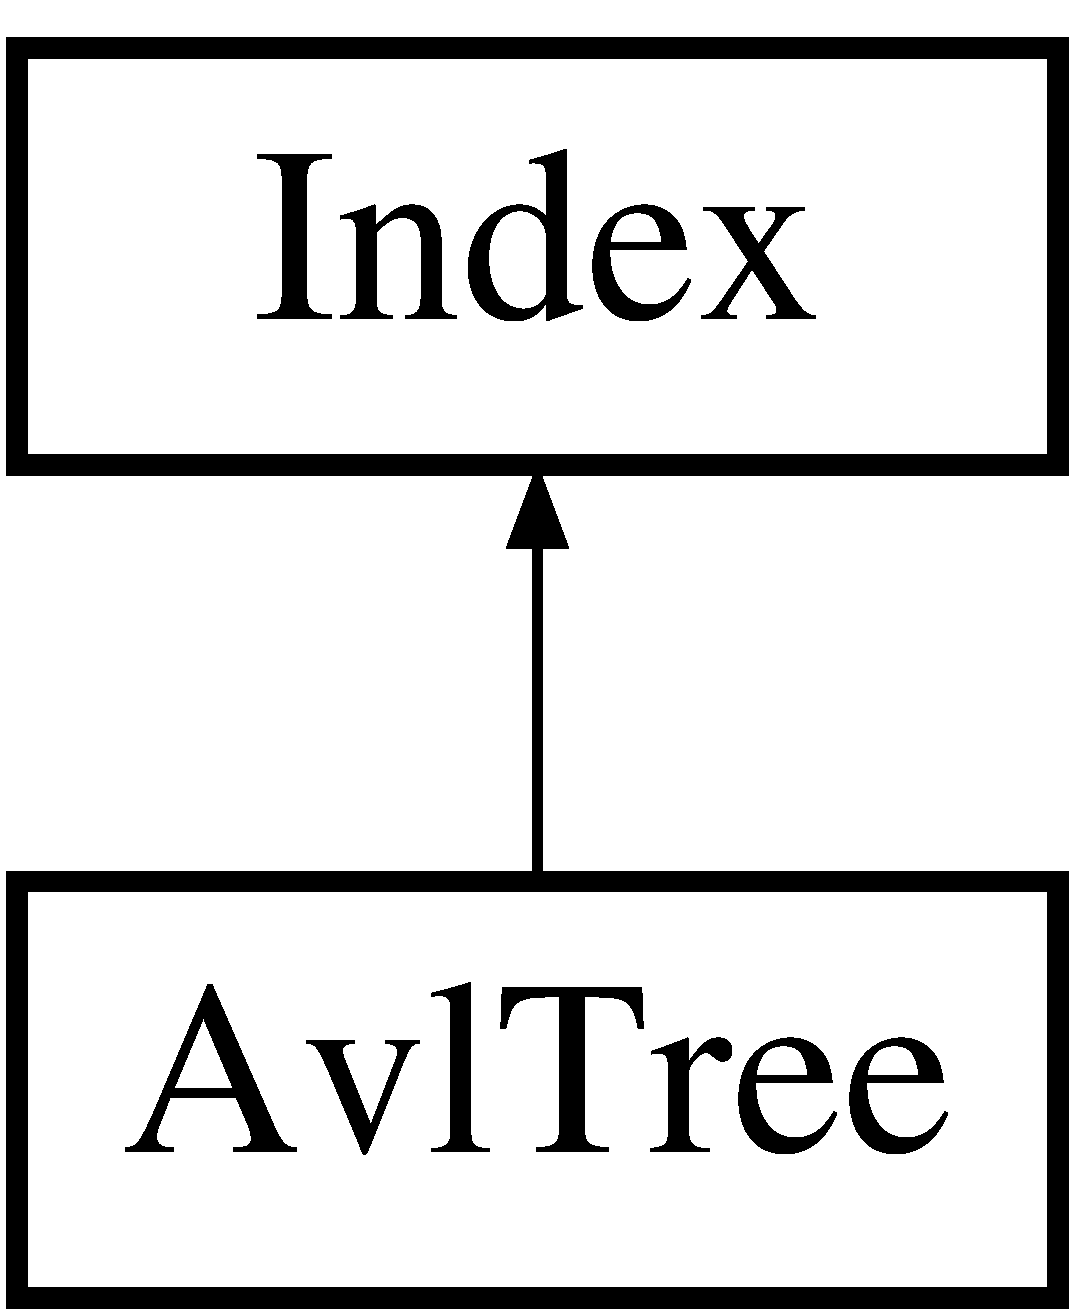
\includegraphics[height=2.000000cm]{class_avl_tree}
\end{center}
\end{figure}
\subsection*{Public Member Functions}
\begin{DoxyCompactItemize}
\item 
\hypertarget{class_avl_tree_a16ffec16dffe9da5c7b7b0faab5b0620}{\hyperlink{class_avl_tree_a16ffec16dffe9da5c7b7b0faab5b0620}{Avl\-Tree} ()}\label{class_avl_tree_a16ffec16dffe9da5c7b7b0faab5b0620}

\begin{DoxyCompactList}\small\item\em \hyperlink{class_avl_tree}{Avl\-Tree} default constructor. \end{DoxyCompactList}\item 
\hypertarget{class_avl_tree_a3c8a14fc5a22671202082edb7999926d}{virtual \hyperlink{class_avl_tree_a3c8a14fc5a22671202082edb7999926d}{$\sim$\-Avl\-Tree} ()}\label{class_avl_tree_a3c8a14fc5a22671202082edb7999926d}

\begin{DoxyCompactList}\small\item\em $\sim$\-Avl\-Tree virtual destructor \end{DoxyCompactList}\item 
\hyperlink{class_avl_tree_a53dc67ed47b09f8d646cc2693b5c9c04}{Avl\-Tree} (const \hyperlink{class_avl_tree}{Avl\-Tree} \&cp)
\begin{DoxyCompactList}\small\item\em \hyperlink{class_avl_tree}{Avl\-Tree} copy constructor. \end{DoxyCompactList}\item 
\hyperlink{class_avl_tree}{Avl\-Tree} \& \hyperlink{class_avl_tree_a1850c4de3588a85f6dfd887b5286527c}{operator=} (const \hyperlink{class_avl_tree}{Avl\-Tree} \&cp)
\begin{DoxyCompactList}\small\item\em operator = overloaded assignment operator. \end{DoxyCompactList}\item 
\hypertarget{class_avl_tree_a63143b0d8570b80dd7290e8280906233}{void \hyperlink{class_avl_tree_a63143b0d8570b80dd7290e8280906233}{clear} ()}\label{class_avl_tree_a63143b0d8570b80dd7290e8280906233}

\begin{DoxyCompactList}\small\item\em clear clears the avl tree. \end{DoxyCompactList}\item 
void \hyperlink{class_avl_tree_a9305ea46f35f021ddf30bbc87c071f30}{insert} (string \&key, int \&pg, double \&freq, string \&header, string \&date, string \&user)
\begin{DoxyCompactList}\small\item\em insert inserts a node into the tree. \end{DoxyCompactList}\item 
void \hyperlink{class_avl_tree_a82a02d204f4067ff89e0fb6925d58893}{insert\-L\-L} (string \&key, \hyperlink{class_linked_list}{Linked\-List} $\ast$\&ll)
\begin{DoxyCompactList}\small\item\em insert\-L\-L inserts a word and linked list into a linked list. \end{DoxyCompactList}\item 
string \& \hyperlink{class_avl_tree_ad2eb1d8582a66fd6fe3af126466aff19}{find\-Keyword} (string \&key)
\begin{DoxyCompactList}\small\item\em find\-Keyword finds a keyword in the tree. \end{DoxyCompactList}\item 
\hyperlink{class_linked_list}{Linked\-List} $\ast$\& \hyperlink{class_avl_tree_a60f76637184e51d2e78c8935ef14aea7}{find\-Data} (string \&key)
\begin{DoxyCompactList}\small\item\em find\-Data finds the data associated with a keyword in the linked list. \end{DoxyCompactList}\item 
int \& \hyperlink{class_avl_tree_a1821114e5e9ef3a482d601d11561853c}{get\-Size} ()
\begin{DoxyCompactList}\small\item\em get\-Size returns the size of the tree. \end{DoxyCompactList}\end{DoxyCompactItemize}


\subsection{Detailed Description}
An Avl Tree with nodes that contain a word, page number, page title, page date, page contributor's username, and a pointer to the next node. 

subclass 

\subsection{Constructor \& Destructor Documentation}
\hypertarget{class_avl_tree_a53dc67ed47b09f8d646cc2693b5c9c04}{\index{Avl\-Tree@{Avl\-Tree}!Avl\-Tree@{Avl\-Tree}}
\index{Avl\-Tree@{Avl\-Tree}!AvlTree@{Avl\-Tree}}
\subsubsection[{Avl\-Tree}]{\setlength{\rightskip}{0pt plus 5cm}Avl\-Tree\-::\-Avl\-Tree (
\begin{DoxyParamCaption}
\item[{const {\bf Avl\-Tree} \&}]{cp}
\end{DoxyParamCaption}
)\hspace{0.3cm}{\ttfamily [inline]}}}\label{class_avl_tree_a53dc67ed47b09f8d646cc2693b5c9c04}


\hyperlink{class_avl_tree}{Avl\-Tree} copy constructor. 


\begin{DoxyParams}{Parameters}
{\em cp} & a constant \hyperlink{class_avl_tree}{Avl\-Tree} object \\
\hline
\end{DoxyParams}


\subsection{Member Function Documentation}
\hypertarget{class_avl_tree_a60f76637184e51d2e78c8935ef14aea7}{\index{Avl\-Tree@{Avl\-Tree}!find\-Data@{find\-Data}}
\index{find\-Data@{find\-Data}!AvlTree@{Avl\-Tree}}
\subsubsection[{find\-Data}]{\setlength{\rightskip}{0pt plus 5cm}{\bf Linked\-List}$\ast$\& Avl\-Tree\-::find\-Data (
\begin{DoxyParamCaption}
\item[{string \&}]{key}
\end{DoxyParamCaption}
)\hspace{0.3cm}{\ttfamily [inline]}, {\ttfamily [virtual]}}}\label{class_avl_tree_a60f76637184e51d2e78c8935ef14aea7}


find\-Data finds the data associated with a keyword in the linked list. 


\begin{DoxyParams}{Parameters}
{\em key} & a string containing a keyword \\
\hline
\end{DoxyParams}
\begin{DoxyReturn}{Returns}
a reference to a linked list pointer 
\end{DoxyReturn}


Implements \hyperlink{class_index_a72c1cd00b6fce902a5d08e9278954913}{Index}.

\hypertarget{class_avl_tree_ad2eb1d8582a66fd6fe3af126466aff19}{\index{Avl\-Tree@{Avl\-Tree}!find\-Keyword@{find\-Keyword}}
\index{find\-Keyword@{find\-Keyword}!AvlTree@{Avl\-Tree}}
\subsubsection[{find\-Keyword}]{\setlength{\rightskip}{0pt plus 5cm}string\& Avl\-Tree\-::find\-Keyword (
\begin{DoxyParamCaption}
\item[{string \&}]{key}
\end{DoxyParamCaption}
)\hspace{0.3cm}{\ttfamily [inline]}, {\ttfamily [virtual]}}}\label{class_avl_tree_ad2eb1d8582a66fd6fe3af126466aff19}


find\-Keyword finds a keyword in the tree. 


\begin{DoxyParams}{Parameters}
{\em key} & a string containing a keyword \\
\hline
\end{DoxyParams}
\begin{DoxyReturn}{Returns}
a reference to a string 
\end{DoxyReturn}


Implements \hyperlink{class_index_a8ee654f84f96668a451afcf39fe2cc69}{Index}.

\hypertarget{class_avl_tree_a1821114e5e9ef3a482d601d11561853c}{\index{Avl\-Tree@{Avl\-Tree}!get\-Size@{get\-Size}}
\index{get\-Size@{get\-Size}!AvlTree@{Avl\-Tree}}
\subsubsection[{get\-Size}]{\setlength{\rightskip}{0pt plus 5cm}int\& Avl\-Tree\-::get\-Size (
\begin{DoxyParamCaption}
{}
\end{DoxyParamCaption}
)\hspace{0.3cm}{\ttfamily [inline]}, {\ttfamily [virtual]}}}\label{class_avl_tree_a1821114e5e9ef3a482d601d11561853c}


get\-Size returns the size of the tree. 

\begin{DoxyReturn}{Returns}
a reference to an integer 
\end{DoxyReturn}


Implements \hyperlink{class_index_a0eccb696eb6548d60df4a4bce323191b}{Index}.

\hypertarget{class_avl_tree_a9305ea46f35f021ddf30bbc87c071f30}{\index{Avl\-Tree@{Avl\-Tree}!insert@{insert}}
\index{insert@{insert}!AvlTree@{Avl\-Tree}}
\subsubsection[{insert}]{\setlength{\rightskip}{0pt plus 5cm}void Avl\-Tree\-::insert (
\begin{DoxyParamCaption}
\item[{string \&}]{key, }
\item[{int \&}]{pg, }
\item[{double \&}]{freq, }
\item[{string \&}]{header, }
\item[{string \&}]{date, }
\item[{string \&}]{user}
\end{DoxyParamCaption}
)\hspace{0.3cm}{\ttfamily [inline]}, {\ttfamily [virtual]}}}\label{class_avl_tree_a9305ea46f35f021ddf30bbc87c071f30}


insert inserts a node into the tree. 


\begin{DoxyParams}{Parameters}
{\em key} & a string containing a word from the page \\
\hline
{\em pg} & an integer containing the page number \\
\hline
{\em freq} & an integer containing the word frequency \\
\hline
{\em header} & a string containing the page title \\
\hline
{\em date} & a string containing the page date \\
\hline
{\em user} & a string containing the page contributor's username \\
\hline
\end{DoxyParams}


Implements \hyperlink{class_index_ad44792ad4f81ef1e17a0c6cb6f57167c}{Index}.

\hypertarget{class_avl_tree_a82a02d204f4067ff89e0fb6925d58893}{\index{Avl\-Tree@{Avl\-Tree}!insert\-L\-L@{insert\-L\-L}}
\index{insert\-L\-L@{insert\-L\-L}!AvlTree@{Avl\-Tree}}
\subsubsection[{insert\-L\-L}]{\setlength{\rightskip}{0pt plus 5cm}void Avl\-Tree\-::insert\-L\-L (
\begin{DoxyParamCaption}
\item[{string \&}]{key, }
\item[{{\bf Linked\-List} $\ast$\&}]{ll}
\end{DoxyParamCaption}
)\hspace{0.3cm}{\ttfamily [inline]}, {\ttfamily [virtual]}}}\label{class_avl_tree_a82a02d204f4067ff89e0fb6925d58893}


insert\-L\-L inserts a word and linked list into a linked list. 


\begin{DoxyParams}{Parameters}
{\em key} & a string containing a word \\
\hline
{\em ll} & a linked list pointer containing the page number, frequency, page title, page date, and page contributor's username for the word \\
\hline
\end{DoxyParams}


Implements \hyperlink{class_index_a423c014174a0257d27b7e5c5834f92ed}{Index}.

\hypertarget{class_avl_tree_a1850c4de3588a85f6dfd887b5286527c}{\index{Avl\-Tree@{Avl\-Tree}!operator=@{operator=}}
\index{operator=@{operator=}!AvlTree@{Avl\-Tree}}
\subsubsection[{operator=}]{\setlength{\rightskip}{0pt plus 5cm}{\bf Avl\-Tree}\& Avl\-Tree\-::operator= (
\begin{DoxyParamCaption}
\item[{const {\bf Avl\-Tree} \&}]{cp}
\end{DoxyParamCaption}
)\hspace{0.3cm}{\ttfamily [inline]}}}\label{class_avl_tree_a1850c4de3588a85f6dfd887b5286527c}


operator = overloaded assignment operator. 


\begin{DoxyParams}{Parameters}
{\em cp} & a constant \hyperlink{class_avl_tree}{Avl\-Tree} object \\
\hline
\end{DoxyParams}
\begin{DoxyReturn}{Returns}
an \hyperlink{class_avl_tree}{Avl\-Tree} reference 
\end{DoxyReturn}


The documentation for this class was generated from the following file\-:\begin{DoxyCompactItemize}
\item 
avltree.\-h\end{DoxyCompactItemize}

\hypertarget{classbackup__variable}{\section{backup\-\_\-variable$<$ T $>$ Class Template Reference}
\label{classbackup__variable}\index{backup\-\_\-variable$<$ T $>$@{backup\-\_\-variable$<$ T $>$}}
}


class that remembers its original value from construction.  




{\ttfamily \#include $<$utilities.\-h$>$}

\subsection*{Public Member Functions}
\begin{DoxyCompactItemize}
\item 
\hypertarget{classbackup__variable_a5ffb4ce0ce0f679135ce70d8683a9182}{{\bfseries backup\-\_\-variable} (const T \&value)}\label{classbackup__variable_a5ffb4ce0ce0f679135ce70d8683a9182}

\item 
\hypertarget{classbackup__variable_ae4c8c3147d8a341eb268f7b2332098d6}{void {\bfseries operator=} (const T \&value)}\label{classbackup__variable_ae4c8c3147d8a341eb268f7b2332098d6}

\item 
\hypertarget{classbackup__variable_aec3207431e35f74efa6fe2af77ec734d}{bool {\bfseries operator==} (const T \&value) const }\label{classbackup__variable_aec3207431e35f74efa6fe2af77ec734d}

\item 
\hypertarget{classbackup__variable_af6d27d4c48c46816a5f82343609b24db}{bool {\bfseries operator$<$} (const T \&value) const }\label{classbackup__variable_af6d27d4c48c46816a5f82343609b24db}

\item 
\hypertarget{classbackup__variable_a60de5d54f02e5d862ae851ab773830db}{bool {\bfseries operator$<$=} (const T \&value) const }\label{classbackup__variable_a60de5d54f02e5d862ae851ab773830db}

\item 
\hypertarget{classbackup__variable_a1956d30f9a5124527ac9d52821ce9d72}{bool {\bfseries operator$>$} (const T \&value) const }\label{classbackup__variable_a1956d30f9a5124527ac9d52821ce9d72}

\item 
\hypertarget{classbackup__variable_a0b749c6e3c84c43d094d1ba50d1a2323}{bool {\bfseries operator$>$=} (const T \&value) const }\label{classbackup__variable_a0b749c6e3c84c43d094d1ba50d1a2323}

\item 
\hypertarget{classbackup__variable_a1ae3f1fcce3725da51aab2879c523a09}{void {\bfseries operator+} (const T \&value)}\label{classbackup__variable_a1ae3f1fcce3725da51aab2879c523a09}

\item 
\hypertarget{classbackup__variable_a4b5753702dbfdaf23f9eb8b210ed80a2}{void {\bfseries operator+=} (const T \&value)}\label{classbackup__variable_a4b5753702dbfdaf23f9eb8b210ed80a2}

\item 
\hypertarget{classbackup__variable_abc321dce84d827d20d69b96653049739}{void {\bfseries operator-\/} (const T \&value)}\label{classbackup__variable_abc321dce84d827d20d69b96653049739}

\item 
\hypertarget{classbackup__variable_adc890d1d8539089e654280bf18e76034}{void {\bfseries operator-\/=} (const T \&value)}\label{classbackup__variable_adc890d1d8539089e654280bf18e76034}

\item 
\hypertarget{classbackup__variable_acba460a7693d0db536d7f9768ab6cf67}{{\bfseries operator const T} () const }\label{classbackup__variable_acba460a7693d0db536d7f9768ab6cf67}

\item 
\hypertarget{classbackup__variable_a61a6e2eee207d52e8f80f23595615627}{T $\ast$ {\bfseries operator\&} ()}\label{classbackup__variable_a61a6e2eee207d52e8f80f23595615627}

\item 
\hypertarget{classbackup__variable_a636435af2389592a1b96038d83582d8a}{const T \& {\bfseries get\-\_\-value} () const }\label{classbackup__variable_a636435af2389592a1b96038d83582d8a}

\item 
\hypertarget{classbackup__variable_a0338d95a730475c9ec88aff25c76b80f}{T \& {\bfseries get\-\_\-value} ()}\label{classbackup__variable_a0338d95a730475c9ec88aff25c76b80f}

\item 
\hypertarget{classbackup__variable_a4d062c1afac850f6e965ccf6ebdca951}{bool {\bfseries has\-\_\-changed} () const }\label{classbackup__variable_a4d062c1afac850f6e965ccf6ebdca951}

\end{DoxyCompactItemize}


\subsection{Detailed Description}
\subsubsection*{template$<$typename T$>$class backup\-\_\-variable$<$ T $>$}

class that remembers its original value from construction. 

The documentation for this class was generated from the following file\-:\begin{DoxyCompactItemize}
\item 
utilities/utilities.\-h\end{DoxyCompactItemize}

\hypertarget{classcomparable__first__pair}{\section{comparable\-\_\-first\-\_\-pair$<$ T1, T2 $>$ Class Template Reference}
\label{classcomparable__first__pair}\index{comparable\-\_\-first\-\_\-pair$<$ T1, T2 $>$@{comparable\-\_\-first\-\_\-pair$<$ T1, T2 $>$}}
}


pair interface that compares on the first item  




{\ttfamily \#include $<$utilities.\-h$>$}

Inheritance diagram for comparable\-\_\-first\-\_\-pair$<$ T1, T2 $>$\-:\begin{figure}[H]
\begin{center}
\leavevmode
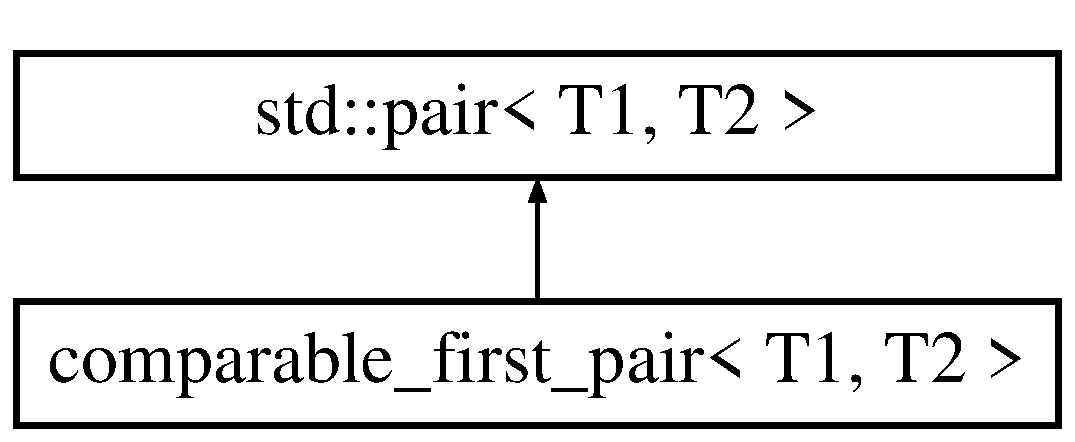
\includegraphics[height=2.000000cm]{classcomparable__first__pair}
\end{center}
\end{figure}
\subsection*{Public Member Functions}
\begin{DoxyCompactItemize}
\item 
\hypertarget{classcomparable__first__pair_a2983fa9fde1ab3b1edc13b8dd37a913a}{{\bfseries comparable\-\_\-first\-\_\-pair} (const T1 \&t1, const T2 \&t2)}\label{classcomparable__first__pair_a2983fa9fde1ab3b1edc13b8dd37a913a}

\item 
\hypertarget{classcomparable__first__pair_a67562f833f477f952e86f4d6dc39e118}{bool {\bfseries operator$<$} (const \hyperlink{classcomparable__first__pair}{comparable\-\_\-first\-\_\-pair}$<$ T1, T2 $>$ \&that) const }\label{classcomparable__first__pair_a67562f833f477f952e86f4d6dc39e118}

\item 
\hypertarget{classcomparable__first__pair_aeb65ed4ea3789b102e7ef750cb72d875}{bool {\bfseries operator==} (const \hyperlink{classcomparable__first__pair}{comparable\-\_\-first\-\_\-pair}$<$ T1, T2 $>$ \&that) const }\label{classcomparable__first__pair_aeb65ed4ea3789b102e7ef750cb72d875}

\end{DoxyCompactItemize}


\subsection{Detailed Description}
\subsubsection*{template$<$typename T1, typename T2$>$class comparable\-\_\-first\-\_\-pair$<$ T1, T2 $>$}

pair interface that compares on the first item 

The documentation for this class was generated from the following file\-:\begin{DoxyCompactItemize}
\item 
utilities/utilities.\-h\end{DoxyCompactItemize}

\hypertarget{class_document_parser}{\section{Document\-Parser Class Reference}
\label{class_document_parser}\index{Document\-Parser@{Document\-Parser}}
}


Parses X\-M\-L Document.  




{\ttfamily \#include $<$documentparser.\-h$>$}

\subsection*{Public Member Functions}
\begin{DoxyCompactItemize}
\item 
\hypertarget{class_document_parser_a7a281448c94759450046ab2fb57e7aae}{\hyperlink{class_document_parser_a7a281448c94759450046ab2fb57e7aae}{Document\-Parser} ()}\label{class_document_parser_a7a281448c94759450046ab2fb57e7aae}

\begin{DoxyCompactList}\small\item\em \hyperlink{class_document_parser}{Document\-Parser} default constructor. \end{DoxyCompactList}\item 
void \hyperlink{class_document_parser_a08f89dbb39ae984c30158a38ac70be17}{read\-Document} (char $\ast$filename)
\begin{DoxyCompactList}\small\item\em reads/parses the xml document \end{DoxyCompactList}\end{DoxyCompactItemize}


\subsection{Detailed Description}
Parses X\-M\-L Document. 

Parses the Wiki\-Books X\-M\-L document using rapidxml libraries. 

\subsection{Member Function Documentation}
\hypertarget{class_document_parser_a08f89dbb39ae984c30158a38ac70be17}{\index{Document\-Parser@{Document\-Parser}!read\-Document@{read\-Document}}
\index{read\-Document@{read\-Document}!DocumentParser@{Document\-Parser}}
\subsubsection[{read\-Document}]{\setlength{\rightskip}{0pt plus 5cm}void Document\-Parser\-::read\-Document (
\begin{DoxyParamCaption}
\item[{char $\ast$}]{filename}
\end{DoxyParamCaption}
)}}\label{class_document_parser_a08f89dbb39ae984c30158a38ac70be17}


reads/parses the xml document 


\begin{DoxyParams}{Parameters}
{\em filename} & a character pointer \\
\hline
\end{DoxyParams}


The documentation for this class was generated from the following files\-:\begin{DoxyCompactItemize}
\item 
documentparser.\-h\item 
documentparser.\-cpp\end{DoxyCompactItemize}

\hypertarget{classdouble__less}{\section{double\-\_\-less Class Reference}
\label{classdouble__less}\index{double\-\_\-less@{double\-\_\-less}}
}


\char`\"{}less\char`\"{} interface for double values.  




{\ttfamily \#include $<$safe\-\_\-math.\-h$>$}

Inheritance diagram for double\-\_\-less\-:\begin{figure}[H]
\begin{center}
\leavevmode
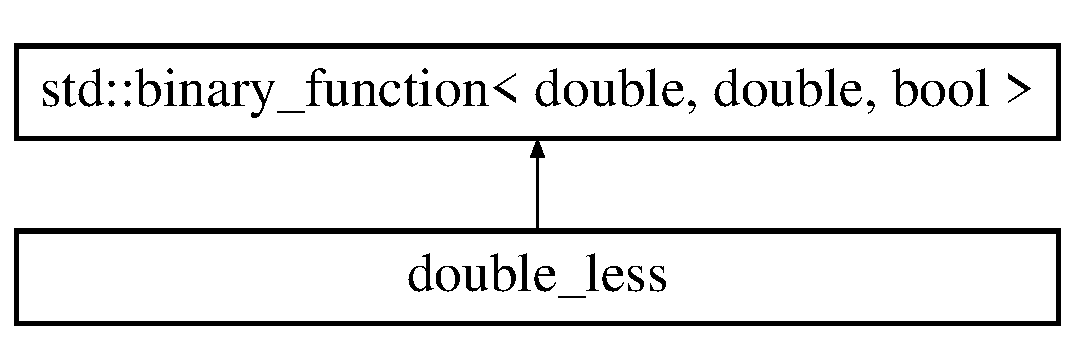
\includegraphics[height=2.000000cm]{classdouble__less}
\end{center}
\end{figure}
\subsection*{Public Member Functions}
\begin{DoxyCompactItemize}
\item 
\hypertarget{group___mathematics_ga8ab290c346a3fa091aac241536ce1c95}{bool {\bfseries operator()} (const double \&left, const double \&right) const }\label{group___mathematics_ga8ab290c346a3fa091aac241536ce1c95}

\end{DoxyCompactItemize}


\subsection{Detailed Description}
\char`\"{}less\char`\"{} interface for double values. 

The documentation for this class was generated from the following file\-:\begin{DoxyCompactItemize}
\item 
utilities/safe\-\_\-math.\-h\end{DoxyCompactItemize}

\hypertarget{classstemming_1_1english__stem}{\section{stemming\-:\-:english\-\_\-stem$<$ string\-\_\-type\-T $>$ Class Template Reference}
\label{classstemming_1_1english__stem}\index{stemming\-::english\-\_\-stem$<$ string\-\_\-type\-T $>$@{stemming\-::english\-\_\-stem$<$ string\-\_\-type\-T $>$}}
}


{\ttfamily \#include $<$english\-\_\-stem.\-h$>$}

Inheritance diagram for stemming\-:\-:english\-\_\-stem$<$ string\-\_\-type\-T $>$\-:\begin{figure}[H]
\begin{center}
\leavevmode
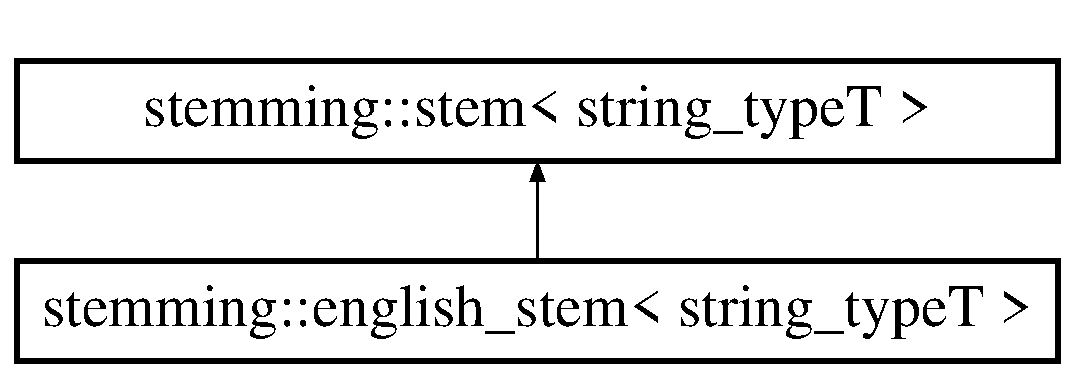
\includegraphics[height=2.000000cm]{classstemming_1_1english__stem}
\end{center}
\end{figure}
\subsection*{Public Member Functions}
\begin{DoxyCompactItemize}
\item 
void \hyperlink{classstemming_1_1english__stem_a8163a8cc4186b749665d616cbf11c492}{operator()} (string\-\_\-type\-T \&text)
\end{DoxyCompactItemize}
\subsection*{Additional Inherited Members}


\subsection{Detailed Description}
\subsubsection*{template$<$typename string\-\_\-type\-T = std\-::wstring$>$class stemming\-::english\-\_\-stem$<$ string\-\_\-type\-T $>$}

Overview

I have made more than one attempt to improve the structure of the Porter algorithm by making it follow the pattern of ending removal of the Romance language stemmers. It is not hard to see why one should want to do this\-: step 1b of the Porter stemmer removes ed and ing, which are i-\/suffixes ($\ast$) attached to verbs. If these suffixes are removed, there should be no need to remove d-\/suffixes which are not verbal, although it will try to do so. This seems to be a deficiency in the Porter stemmer, not shared by the Romance stemmers. Again, the divisions between steps 2, 3 and 4 seem rather arbitrary, and are not found in the Romance stemmers.

Nevertheless, these attempts at improvement have been abandoned. They seem to lead to a more complicated algorithm with no very obvious improvements. A reason for not taking note of the outcome of step 1b may be that English endings do not determine word categories quite as strongly as endings in the Romance languages. For example, condition and position in French have to be nouns, but in English they can be verbs as well as nouns,

We are all conditioned by advertising They are positioning themselves differently today

A possible reason for having separate steps 2, 3 and 4 is that d-\/suffix combinations in English are quite complex, a point which has been made elsewhere.

But it is hardly surprising that after twenty years of use of the Porter stemmer, certain improvements do suggest themselves, and a new algorithm for English is therefore offered here. (It could be called the 'Porter2' stemmer to distinguish it from the Porter stemmer, from which it derives.) The changes are not so very extensive\-: (1) terminating y is changed to i rather less often, (2) suffix us does not lose its s, (3) a few additional suffixes are included for removal, including (4) suffix ly. In addition, a small list of exceptional forms is included. In December 2001 there were two further adjustments\-: (5) Steps 5a and 5b of the old Porter stemmer were combined into a single step. This means that undoubling final ll is not done with removal of final e. (6) In Step 3 ative is removed only when in region R2.

To begin with, here is the basic algorithm without reference to the exceptional forms. An exact comparison with the Porter algorithm needs to be done quite carefully if done at all. Here we indicate by $\ast$ points of departure, and by + additional features. In the sample vocabulary, Porter and Porter2 stem slightly under 5\% of words to different forms.

Dr. Martin Porter

Define a vowel as one of
\begin{DoxyItemize}
\item a e i o u y
\end{DoxyItemize}

Define a double as one of
\begin{DoxyItemize}
\item bb dd ff gg mm nn pp rr tt
\end{DoxyItemize}

Define a valid li-\/ending as one of
\begin{DoxyItemize}
\item c d e g h k m n r t
\end{DoxyItemize}

Define a short syllable in a word as either (a) a vowel followed by a non-\/vowel other than w, x or Y and preceded by a non-\/vowel, or $\ast$ (b) a vowel at the beginning of the word followed by a non-\/vowel.

So rap, trap, entrap end with a short syllable, and ow, on, at are classed as short syllables. But uproot, bestow, disturb do not end with a short syllable.

A word is called short if it consists of a short syllable preceded by zero or more consonants. R1 is the region after the first non-\/vowel following a vowel, or the end of the word if there is no such non-\/vowel. R2 is the region after the first non-\/vowel following a vowel in R1, or the end of the word if there is no such non-\/vowel. If the word has two letters or less, leave it as it is. Otherwise, do each of the following operations, Set initial y, or y after a vowel, to Y, and then establish the regions R1 and R2.

\begin{DoxyParagraph}{Algorithm\-:}

\end{DoxyParagraph}
{\bfseries Step 1a\-:}

Search for the longest among the following suffixes, and perform the action indicated\-:
\begin{DoxyItemize}
\item sses
\begin{DoxyItemize}
\item Replace by ss.
\end{DoxyItemize}
\item ied+ ies$\ast$
\begin{DoxyItemize}
\item Replace by i if preceded by just one letter, otherwise by ie (so ties -\/$>$ tie, cries -\/$>$ cri).
\end{DoxyItemize}
\item s
\begin{DoxyItemize}
\item Delete if the preceding word part contains a vowel not immediately before the s (so gas and this retain the s, gaps and kiwis lose it).
\end{DoxyItemize}
\item us+ ss
\begin{DoxyItemize}
\item Do nothing.
\end{DoxyItemize}
\end{DoxyItemize}

{\bfseries Step 1b\-:}

Search for the longest among the following suffixes, and perform the action indicated\-:
\begin{DoxyItemize}
\item eed eedly+
\begin{DoxyItemize}
\item Replace by ee if in R1.
\end{DoxyItemize}
\item ed edly+ ing ingly+
\begin{DoxyItemize}
\item Delete if the preceding word part contains a vowel, and then
\item If the word ends at, bl or iz add e (so luxuriat -\/$>$ luxuriate), or
\item If the word ends with a double remove the last letter (so hopp -\/$>$ hop), or
\item If the word is short, add e (so hop -\/$>$ hope).
\end{DoxyItemize}
\end{DoxyItemize}

{\bfseries Step 1c\-:}

Replace suffix y or Y by i if preceded by a non-\/vowel which is not the first letter of the word (so cry -\/$>$ cri, by -\/$>$ by, say -\/$>$ say)

{\bfseries Step 2\-:}

Search for the longest among the following suffixes, and, if found and in R1, perform the action indicated\-:
\begin{DoxyItemize}
\item tional
\begin{DoxyItemize}
\item Replace by tion.
\end{DoxyItemize}
\item enci
\begin{DoxyItemize}
\item Replace by ence.
\end{DoxyItemize}
\item anci
\begin{DoxyItemize}
\item Replace by ance
\end{DoxyItemize}
\item abli
\begin{DoxyItemize}
\item Replace by able.
\end{DoxyItemize}
\item entli
\begin{DoxyItemize}
\item Replace by ent.
\end{DoxyItemize}
\item izer ization
\begin{DoxyItemize}
\item Replace by ize.
\end{DoxyItemize}
\item ational ation ator
\begin{DoxyItemize}
\item Replace by ate.
\end{DoxyItemize}
\item alism aliti alli
\begin{DoxyItemize}
\item Replace by al.
\end{DoxyItemize}
\item fulness
\begin{DoxyItemize}
\item Replace by ful.
\end{DoxyItemize}
\item ousli ousness
\begin{DoxyItemize}
\item Replace by ous.
\end{DoxyItemize}
\item iveness iviti
\begin{DoxyItemize}
\item Replace by ive.
\end{DoxyItemize}
\item biliti bli+
\begin{DoxyItemize}
\item Replace by ble.
\end{DoxyItemize}
\item ogi+
\begin{DoxyItemize}
\item Replace by og if preceded by l.
\end{DoxyItemize}
\item fulli+
\begin{DoxyItemize}
\item Replace by ful.
\end{DoxyItemize}
\item lessli+
\begin{DoxyItemize}
\item Replace by less.
\end{DoxyItemize}
\item li+
\begin{DoxyItemize}
\item Delete if preceded by a valid li-\/ending.
\end{DoxyItemize}
\end{DoxyItemize}

{\bfseries Step 3\-:}

Search for the longest among the following suffixes, and, if found and in R1, perform the action indicated\-:
\begin{DoxyItemize}
\item tional+
\begin{DoxyItemize}
\item Replace by tion.
\end{DoxyItemize}
\item ational+
\begin{DoxyItemize}
\item Replace by ate.
\end{DoxyItemize}
\item alize
\begin{DoxyItemize}
\item Replace by al.
\end{DoxyItemize}
\item icate iciti ical
\begin{DoxyItemize}
\item Replace by ic.
\end{DoxyItemize}
\item ful ness
\begin{DoxyItemize}
\item Delete.
\end{DoxyItemize}
\item ative$\ast$
\begin{DoxyItemize}
\item Delete if in R2.
\end{DoxyItemize}
\end{DoxyItemize}

{\bfseries Step 4\-:}

Search for the longest among the following suffixes, and, if found and in R2, perform the action indicated\-:
\begin{DoxyItemize}
\item al ance ence er ic able ible ant ement ment ent ism ate iti ous ive ize
\begin{DoxyItemize}
\item Delete
\end{DoxyItemize}
\item ion
\begin{DoxyItemize}
\item Delete if preceded by s or t.
\end{DoxyItemize}
\end{DoxyItemize}

{\bfseries Step 5\-:}

Search for the following suffixes, and, if found, perform the action indicated\-:
\begin{DoxyItemize}
\item e
\begin{DoxyItemize}
\item Delete if in R2, or in R1 and not preceded by a short syllable.
\end{DoxyItemize}
\item l
\begin{DoxyItemize}
\item Delete if in R2 and preceded by l. 
\end{DoxyItemize}
\end{DoxyItemize}

\subsection{Member Function Documentation}
\hypertarget{classstemming_1_1english__stem_a8163a8cc4186b749665d616cbf11c492}{\index{stemming\-::english\-\_\-stem@{stemming\-::english\-\_\-stem}!operator()@{operator()}}
\index{operator()@{operator()}!stemming::english_stem@{stemming\-::english\-\_\-stem}}
\subsubsection[{operator()}]{\setlength{\rightskip}{0pt plus 5cm}template$<$typename string\-\_\-type\-T  = std\-::wstring$>$ void {\bf stemming\-::english\-\_\-stem}$<$ string\-\_\-type\-T $>$\-::operator() (
\begin{DoxyParamCaption}
\item[{string\-\_\-type\-T \&}]{text}
\end{DoxyParamCaption}
)\hspace{0.3cm}{\ttfamily [inline]}}}\label{classstemming_1_1english__stem_a8163a8cc4186b749665d616cbf11c492}

\begin{DoxyParams}[1]{Parameters}
\mbox{\tt in,out}  & {\em text} & English string to stem. \\
\hline
\end{DoxyParams}


The documentation for this class was generated from the following file\-:\begin{DoxyCompactItemize}
\item 
stemming/english\-\_\-stem.\-h\end{DoxyCompactItemize}

\hypertarget{classstring__util_1_1equal__basic__string__i__compare}{\section{string\-\_\-util\-:\-:equal\-\_\-basic\-\_\-string\-\_\-i\-\_\-compare$<$ T $>$ Class Template Reference}
\label{classstring__util_1_1equal__basic__string__i__compare}\index{string\-\_\-util\-::equal\-\_\-basic\-\_\-string\-\_\-i\-\_\-compare$<$ T $>$@{string\-\_\-util\-::equal\-\_\-basic\-\_\-string\-\_\-i\-\_\-compare$<$ T $>$}}
}
Inheritance diagram for string\-\_\-util\-:\-:equal\-\_\-basic\-\_\-string\-\_\-i\-\_\-compare$<$ T $>$\-:\begin{figure}[H]
\begin{center}
\leavevmode
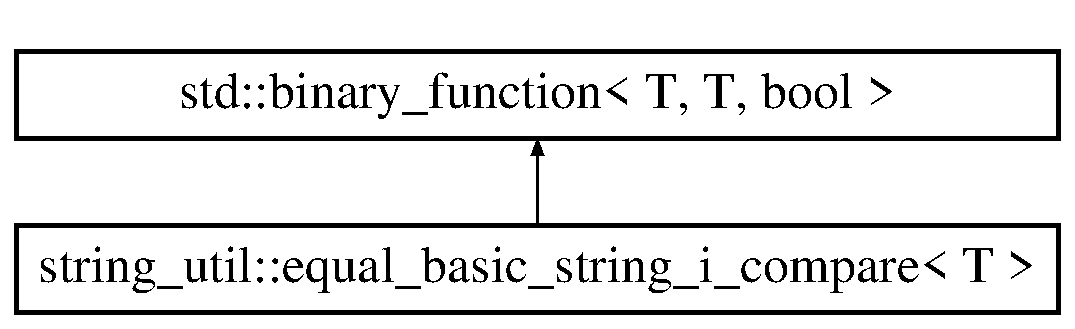
\includegraphics[height=2.000000cm]{classstring__util_1_1equal__basic__string__i__compare}
\end{center}
\end{figure}
\subsection*{Public Member Functions}
\begin{DoxyCompactItemize}
\item 
\hypertarget{classstring__util_1_1equal__basic__string__i__compare_a29fabe519d28908f5b72dcb799cac64f}{bool {\bfseries operator()} (const T \&a\-\_\-, const T \&b\-\_\-) const }\label{classstring__util_1_1equal__basic__string__i__compare_a29fabe519d28908f5b72dcb799cac64f}

\end{DoxyCompactItemize}


The documentation for this class was generated from the following file\-:\begin{DoxyCompactItemize}
\item 
indexing/string\-\_\-util.\-h\end{DoxyCompactItemize}

\hypertarget{classstring__util_1_1equal__string__compare}{\section{string\-\_\-util\-:\-:equal\-\_\-string\-\_\-compare$<$ T $>$ Class Template Reference}
\label{classstring__util_1_1equal__string__compare}\index{string\-\_\-util\-::equal\-\_\-string\-\_\-compare$<$ T $>$@{string\-\_\-util\-::equal\-\_\-string\-\_\-compare$<$ T $>$}}
}
Inheritance diagram for string\-\_\-util\-:\-:equal\-\_\-string\-\_\-compare$<$ T $>$\-:\begin{figure}[H]
\begin{center}
\leavevmode
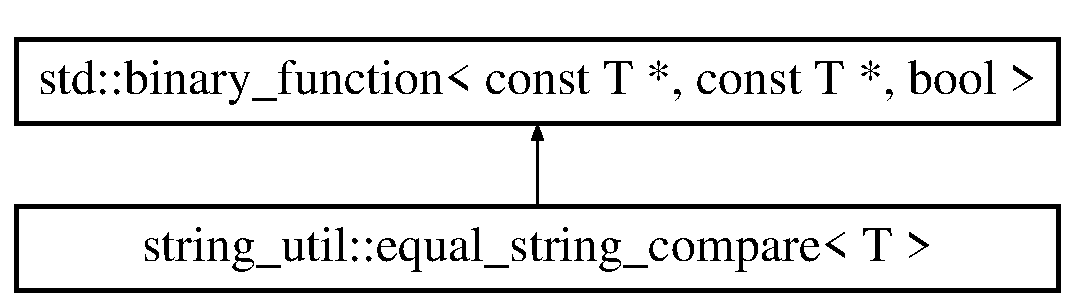
\includegraphics[height=2.000000cm]{classstring__util_1_1equal__string__compare}
\end{center}
\end{figure}
\subsection*{Public Member Functions}
\begin{DoxyCompactItemize}
\item 
\hypertarget{classstring__util_1_1equal__string__compare_aedfb40c0515b97043369af03da1d72ed}{bool {\bfseries operator()} (const T $\ast$a\-\_\-, const T $\ast$b\-\_\-) const }\label{classstring__util_1_1equal__string__compare_aedfb40c0515b97043369af03da1d72ed}

\end{DoxyCompactItemize}


The documentation for this class was generated from the following file\-:\begin{DoxyCompactItemize}
\item 
indexing/string\-\_\-util.\-h\end{DoxyCompactItemize}

\hypertarget{classstring__util_1_1equal__string__i__compare}{\section{string\-\_\-util\-:\-:equal\-\_\-string\-\_\-i\-\_\-compare$<$ T $>$ Class Template Reference}
\label{classstring__util_1_1equal__string__i__compare}\index{string\-\_\-util\-::equal\-\_\-string\-\_\-i\-\_\-compare$<$ T $>$@{string\-\_\-util\-::equal\-\_\-string\-\_\-i\-\_\-compare$<$ T $>$}}
}
Inheritance diagram for string\-\_\-util\-:\-:equal\-\_\-string\-\_\-i\-\_\-compare$<$ T $>$\-:\begin{figure}[H]
\begin{center}
\leavevmode
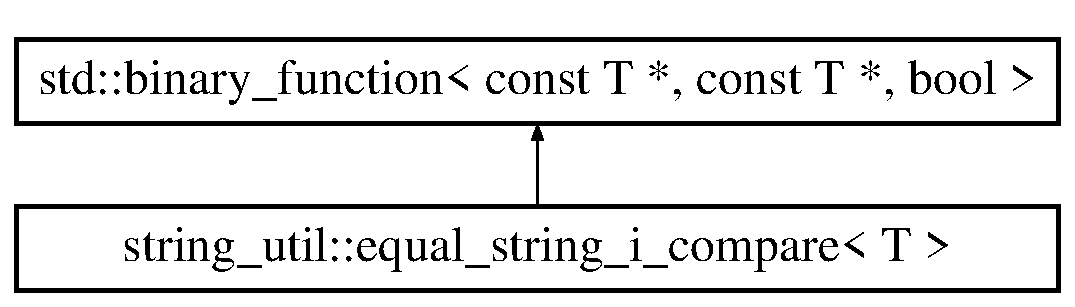
\includegraphics[height=2.000000cm]{classstring__util_1_1equal__string__i__compare}
\end{center}
\end{figure}
\subsection*{Public Member Functions}
\begin{DoxyCompactItemize}
\item 
\hypertarget{classstring__util_1_1equal__string__i__compare_af8c94159bbb8903c7cf7b71941a7d2bc}{bool {\bfseries operator()} (const T $\ast$a\-\_\-, const T $\ast$b\-\_\-) const }\label{classstring__util_1_1equal__string__i__compare_af8c94159bbb8903c7cf7b71941a7d2bc}

\end{DoxyCompactItemize}


The documentation for this class was generated from the following file\-:\begin{DoxyCompactItemize}
\item 
indexing/string\-\_\-util.\-h\end{DoxyCompactItemize}

\hypertarget{classrapidxml_1_1file}{\section{rapidxml\-:\-:file$<$ Ch $>$ Class Template Reference}
\label{classrapidxml_1_1file}\index{rapidxml\-::file$<$ Ch $>$@{rapidxml\-::file$<$ Ch $>$}}
}


Represents data loaded from a file.  




{\ttfamily \#include $<$rapidxml\-\_\-utils.\-hpp$>$}

\subsection*{Public Member Functions}
\begin{DoxyCompactItemize}
\item 
\hyperlink{classrapidxml_1_1file_ae881a3cab1fe7152d45c92a8d7606cb3}{file} (const char $\ast$filename)
\item 
\hyperlink{classrapidxml_1_1file_a90707ccd991cc392dcf4bef37eed9d1f}{file} (std\-::basic\-\_\-istream$<$ Ch $>$ \&stream)
\item 
Ch $\ast$ \hyperlink{classrapidxml_1_1file_af1c71d65862c7af14e4708e32a80c1de}{data} ()
\item 
const Ch $\ast$ \hyperlink{classrapidxml_1_1file_aceb8f5ebd577c946a74b1ea3e2e0c576}{data} () const 
\item 
std\-::size\-\_\-t \hyperlink{classrapidxml_1_1file_a20191d167c6e00a88a44ca9a3a54e1c5}{size} () const 
\end{DoxyCompactItemize}


\subsection{Detailed Description}
\subsubsection*{template$<$class Ch = char$>$class rapidxml\-::file$<$ Ch $>$}

Represents data loaded from a file. 

\subsection{Constructor \& Destructor Documentation}
\hypertarget{classrapidxml_1_1file_ae881a3cab1fe7152d45c92a8d7606cb3}{\index{rapidxml\-::file@{rapidxml\-::file}!file@{file}}
\index{file@{file}!rapidxml::file@{rapidxml\-::file}}
\subsubsection[{file}]{\setlength{\rightskip}{0pt plus 5cm}template$<$class Ch  = char$>$ {\bf rapidxml\-::file}$<$ Ch $>$\-::{\bf file} (
\begin{DoxyParamCaption}
\item[{const char $\ast$}]{filename}
\end{DoxyParamCaption}
)\hspace{0.3cm}{\ttfamily [inline]}}}\label{classrapidxml_1_1file_ae881a3cab1fe7152d45c92a8d7606cb3}
Loads file into the memory. Data will be automatically destroyed by the destructor. 
\begin{DoxyParams}{Parameters}
{\em filename} & Filename to load. \\
\hline
\end{DoxyParams}
\hypertarget{classrapidxml_1_1file_a90707ccd991cc392dcf4bef37eed9d1f}{\index{rapidxml\-::file@{rapidxml\-::file}!file@{file}}
\index{file@{file}!rapidxml::file@{rapidxml\-::file}}
\subsubsection[{file}]{\setlength{\rightskip}{0pt plus 5cm}template$<$class Ch  = char$>$ {\bf rapidxml\-::file}$<$ Ch $>$\-::{\bf file} (
\begin{DoxyParamCaption}
\item[{std\-::basic\-\_\-istream$<$ Ch $>$ \&}]{stream}
\end{DoxyParamCaption}
)\hspace{0.3cm}{\ttfamily [inline]}}}\label{classrapidxml_1_1file_a90707ccd991cc392dcf4bef37eed9d1f}
Loads file into the memory. Data will be automatically destroyed by the destructor 
\begin{DoxyParams}{Parameters}
{\em stream} & Stream to load from \\
\hline
\end{DoxyParams}


\subsection{Member Function Documentation}
\hypertarget{classrapidxml_1_1file_af1c71d65862c7af14e4708e32a80c1de}{\index{rapidxml\-::file@{rapidxml\-::file}!data@{data}}
\index{data@{data}!rapidxml::file@{rapidxml\-::file}}
\subsubsection[{data}]{\setlength{\rightskip}{0pt plus 5cm}template$<$class Ch  = char$>$ Ch$\ast$ {\bf rapidxml\-::file}$<$ Ch $>$\-::data (
\begin{DoxyParamCaption}
{}
\end{DoxyParamCaption}
)\hspace{0.3cm}{\ttfamily [inline]}}}\label{classrapidxml_1_1file_af1c71d65862c7af14e4708e32a80c1de}
Gets file data. \begin{DoxyReturn}{Returns}
Pointer to data of file. 
\end{DoxyReturn}
\hypertarget{classrapidxml_1_1file_aceb8f5ebd577c946a74b1ea3e2e0c576}{\index{rapidxml\-::file@{rapidxml\-::file}!data@{data}}
\index{data@{data}!rapidxml::file@{rapidxml\-::file}}
\subsubsection[{data}]{\setlength{\rightskip}{0pt plus 5cm}template$<$class Ch  = char$>$ const Ch$\ast$ {\bf rapidxml\-::file}$<$ Ch $>$\-::data (
\begin{DoxyParamCaption}
{}
\end{DoxyParamCaption}
) const\hspace{0.3cm}{\ttfamily [inline]}}}\label{classrapidxml_1_1file_aceb8f5ebd577c946a74b1ea3e2e0c576}
Gets file data. \begin{DoxyReturn}{Returns}
Pointer to data of file. 
\end{DoxyReturn}
\hypertarget{classrapidxml_1_1file_a20191d167c6e00a88a44ca9a3a54e1c5}{\index{rapidxml\-::file@{rapidxml\-::file}!size@{size}}
\index{size@{size}!rapidxml::file@{rapidxml\-::file}}
\subsubsection[{size}]{\setlength{\rightskip}{0pt plus 5cm}template$<$class Ch  = char$>$ std\-::size\-\_\-t {\bf rapidxml\-::file}$<$ Ch $>$\-::size (
\begin{DoxyParamCaption}
{}
\end{DoxyParamCaption}
) const\hspace{0.3cm}{\ttfamily [inline]}}}\label{classrapidxml_1_1file_a20191d167c6e00a88a44ca9a3a54e1c5}
Gets file data size. \begin{DoxyReturn}{Returns}
Size of file data, in characters. 
\end{DoxyReturn}


The documentation for this class was generated from the following file\-:\begin{DoxyCompactItemize}
\item 
rapidxml/\hyperlink{rapidxml__utils_8hpp}{rapidxml\-\_\-utils.\-hpp}\end{DoxyCompactItemize}

\hypertarget{class_hash_table}{\section{Hash\-Table Class Reference}
\label{class_hash_table}\index{Hash\-Table@{Hash\-Table}}
}


contains contain a word, page number, page title, page date, and page contributor's username for each page.  


Inheritance diagram for Hash\-Table\-:\begin{figure}[H]
\begin{center}
\leavevmode
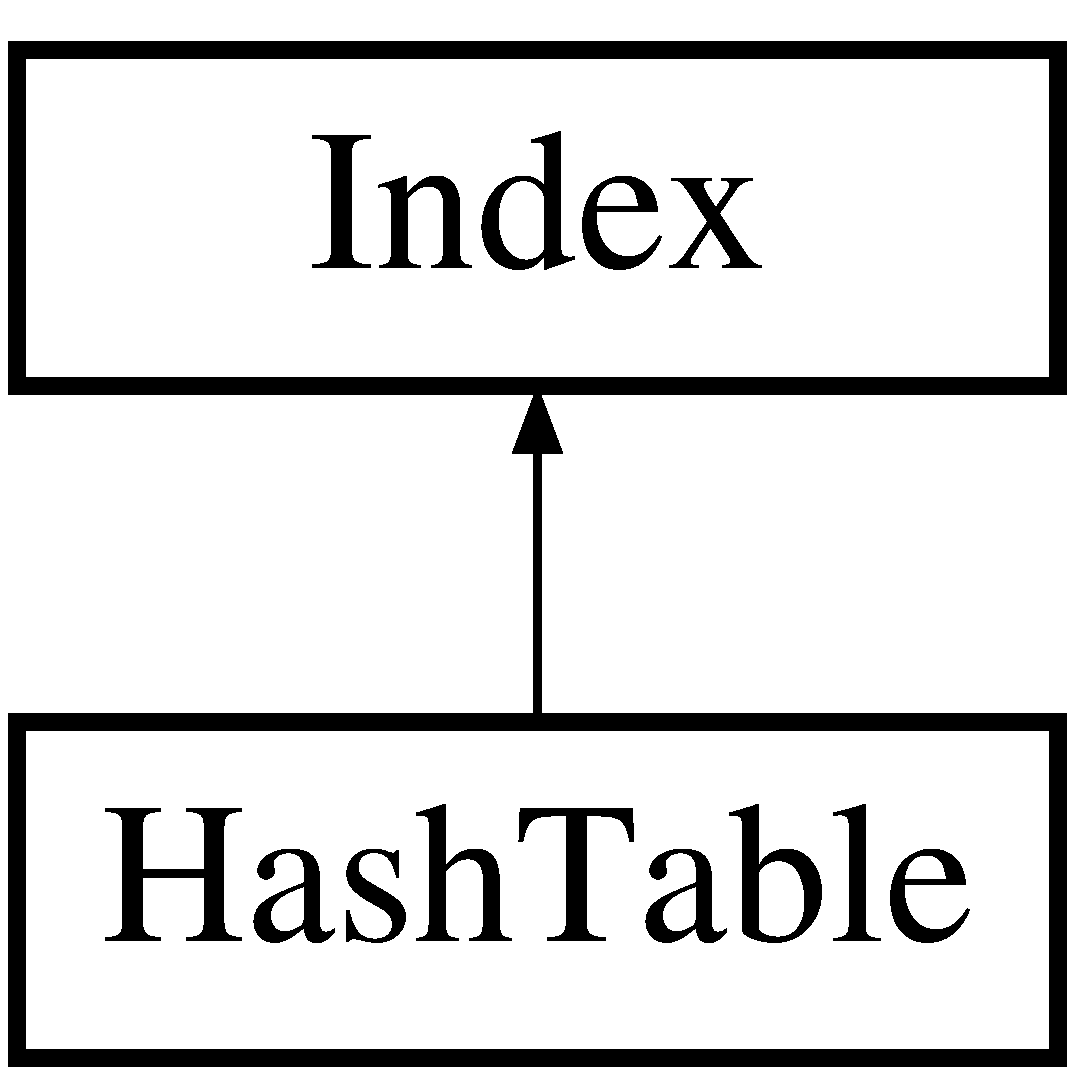
\includegraphics[height=2.000000cm]{class_hash_table}
\end{center}
\end{figure}
\subsection*{Public Member Functions}
\begin{DoxyCompactItemize}
\item 
\hypertarget{class_hash_table_adc3bf2b214c572819ba957ad314d7db3}{\hyperlink{class_hash_table_adc3bf2b214c572819ba957ad314d7db3}{Hash\-Table} ()}\label{class_hash_table_adc3bf2b214c572819ba957ad314d7db3}

\begin{DoxyCompactList}\small\item\em \hyperlink{class_hash_table}{Hash\-Table} default constructor. \end{DoxyCompactList}\item 
\hyperlink{class_hash_table_ac756b78d1ca5e613d68800b76c9bc55c}{Hash\-Table} (const \hyperlink{class_hash_table}{Hash\-Table} \&cp)
\begin{DoxyCompactList}\small\item\em \hyperlink{class_hash_table}{Hash\-Table} copy constructor. \end{DoxyCompactList}\item 
\hyperlink{class_hash_table}{Hash\-Table} \& \hyperlink{class_hash_table_aa8ac131a52516b8cb16530584bdfb021}{operator=} (const \hyperlink{class_hash_table}{Hash\-Table} \&cp)
\begin{DoxyCompactList}\small\item\em operator = overloaded assignment operator \end{DoxyCompactList}\item 
\hypertarget{class_hash_table_adc1d238b66fad676ed683172d8967f46}{virtual \hyperlink{class_hash_table_adc1d238b66fad676ed683172d8967f46}{$\sim$\-Hash\-Table} ()}\label{class_hash_table_adc1d238b66fad676ed683172d8967f46}

\begin{DoxyCompactList}\small\item\em $\sim$\-Hash\-Table \hyperlink{class_hash_table}{Hash\-Table} virtual destructor \end{DoxyCompactList}\item 
\hypertarget{class_hash_table_a94a35e0cf2ce6fa291d48138f58635ed}{void \hyperlink{class_hash_table_a94a35e0cf2ce6fa291d48138f58635ed}{clear} ()}\label{class_hash_table_a94a35e0cf2ce6fa291d48138f58635ed}

\begin{DoxyCompactList}\small\item\em clear clears all the buckets in the hash table. \end{DoxyCompactList}\item 
void \hyperlink{class_hash_table_a3a194bb56855eb892b24455094a1edbb}{insert} (string \&keyword, int \&page\-Number, double \&freq, string \&header, string \&date, string \&user)
\begin{DoxyCompactList}\small\item\em insert all the information into a node. \end{DoxyCompactList}\item 
void \hyperlink{class_hash_table_a096c63eedf8e85a5523d59929f7a7cb3}{insert\-L\-L} (string \&keyword, \hyperlink{class_linked_list}{Linked\-List} $\ast$\&ll)
\begin{DoxyCompactList}\small\item\em insert\-L\-L inserts a word and linked list into a linked list. \end{DoxyCompactList}\item 
void \hyperlink{class_hash_table_afc9f7516810e364c4a8ebed516cd6406}{set\-Hash\-Value} (string \&keyword)
\begin{DoxyCompactList}\small\item\em set\-Hash\-Value sets a hash value for a word used to insert into a bucket. \end{DoxyCompactList}\item 
int \& \hyperlink{class_hash_table_a1968cb702792b31d8b259ce4b945543f}{get\-Size} ()
\begin{DoxyCompactList}\small\item\em get\-Size returns the size of the hash table \end{DoxyCompactList}\item 
string \& \hyperlink{class_hash_table_ab7d96c3bdf0871e7aec5c3fa71a6455c}{find\-Keyword} (string \&keyword)
\begin{DoxyCompactList}\small\item\em find\-Keyword finds a keyword in a node in the hash table. \end{DoxyCompactList}\item 
\hyperlink{class_linked_list}{Linked\-List} $\ast$\& \hyperlink{class_hash_table_a416e1aae0ecadc989c72d0e6b340a8a8}{find\-Data} (string \&keyword)
\begin{DoxyCompactList}\small\item\em find\-Data finds the data associated with a keyword in the linked list. \end{DoxyCompactList}\end{DoxyCompactItemize}


\subsection{Detailed Description}
contains contain a word, page number, page title, page date, and page contributor's username for each page. 

subclass 

\subsection{Constructor \& Destructor Documentation}
\hypertarget{class_hash_table_ac756b78d1ca5e613d68800b76c9bc55c}{\index{Hash\-Table@{Hash\-Table}!Hash\-Table@{Hash\-Table}}
\index{Hash\-Table@{Hash\-Table}!HashTable@{Hash\-Table}}
\subsubsection[{Hash\-Table}]{\setlength{\rightskip}{0pt plus 5cm}Hash\-Table\-::\-Hash\-Table (
\begin{DoxyParamCaption}
\item[{const {\bf Hash\-Table} \&}]{cp}
\end{DoxyParamCaption}
)\hspace{0.3cm}{\ttfamily [inline]}}}\label{class_hash_table_ac756b78d1ca5e613d68800b76c9bc55c}


\hyperlink{class_hash_table}{Hash\-Table} copy constructor. 


\begin{DoxyParams}{Parameters}
{\em cp} & a constant \hyperlink{class_hash_table}{Hash\-Table} object \\
\hline
\end{DoxyParams}


\subsection{Member Function Documentation}
\hypertarget{class_hash_table_a416e1aae0ecadc989c72d0e6b340a8a8}{\index{Hash\-Table@{Hash\-Table}!find\-Data@{find\-Data}}
\index{find\-Data@{find\-Data}!HashTable@{Hash\-Table}}
\subsubsection[{find\-Data}]{\setlength{\rightskip}{0pt plus 5cm}{\bf Linked\-List}$\ast$\& Hash\-Table\-::find\-Data (
\begin{DoxyParamCaption}
\item[{string \&}]{keyword}
\end{DoxyParamCaption}
)\hspace{0.3cm}{\ttfamily [inline]}, {\ttfamily [virtual]}}}\label{class_hash_table_a416e1aae0ecadc989c72d0e6b340a8a8}


find\-Data finds the data associated with a keyword in the linked list. 


\begin{DoxyParams}{Parameters}
{\em keyword} & a string containing a keyword \\
\hline
\end{DoxyParams}
\begin{DoxyReturn}{Returns}
a reference to a linked list pointer 
\end{DoxyReturn}


Implements \hyperlink{class_index_a72c1cd00b6fce902a5d08e9278954913}{Index}.

\hypertarget{class_hash_table_ab7d96c3bdf0871e7aec5c3fa71a6455c}{\index{Hash\-Table@{Hash\-Table}!find\-Keyword@{find\-Keyword}}
\index{find\-Keyword@{find\-Keyword}!HashTable@{Hash\-Table}}
\subsubsection[{find\-Keyword}]{\setlength{\rightskip}{0pt plus 5cm}string\& Hash\-Table\-::find\-Keyword (
\begin{DoxyParamCaption}
\item[{string \&}]{keyword}
\end{DoxyParamCaption}
)\hspace{0.3cm}{\ttfamily [inline]}, {\ttfamily [virtual]}}}\label{class_hash_table_ab7d96c3bdf0871e7aec5c3fa71a6455c}


find\-Keyword finds a keyword in a node in the hash table. 


\begin{DoxyParams}{Parameters}
{\em keyword} & a string containing a word \\
\hline
\end{DoxyParams}
\begin{DoxyReturn}{Returns}

\end{DoxyReturn}


Implements \hyperlink{class_index_a8ee654f84f96668a451afcf39fe2cc69}{Index}.

\hypertarget{class_hash_table_a1968cb702792b31d8b259ce4b945543f}{\index{Hash\-Table@{Hash\-Table}!get\-Size@{get\-Size}}
\index{get\-Size@{get\-Size}!HashTable@{Hash\-Table}}
\subsubsection[{get\-Size}]{\setlength{\rightskip}{0pt plus 5cm}int\& Hash\-Table\-::get\-Size (
\begin{DoxyParamCaption}
{}
\end{DoxyParamCaption}
)\hspace{0.3cm}{\ttfamily [inline]}, {\ttfamily [virtual]}}}\label{class_hash_table_a1968cb702792b31d8b259ce4b945543f}


get\-Size returns the size of the hash table 

\begin{DoxyReturn}{Returns}
an integer reference 
\end{DoxyReturn}


Implements \hyperlink{class_index_a0eccb696eb6548d60df4a4bce323191b}{Index}.

\hypertarget{class_hash_table_a3a194bb56855eb892b24455094a1edbb}{\index{Hash\-Table@{Hash\-Table}!insert@{insert}}
\index{insert@{insert}!HashTable@{Hash\-Table}}
\subsubsection[{insert}]{\setlength{\rightskip}{0pt plus 5cm}void Hash\-Table\-::insert (
\begin{DoxyParamCaption}
\item[{string \&}]{keyword, }
\item[{int \&}]{page\-Number, }
\item[{double \&}]{freq, }
\item[{string \&}]{header, }
\item[{string \&}]{date, }
\item[{string \&}]{user}
\end{DoxyParamCaption}
)\hspace{0.3cm}{\ttfamily [inline]}, {\ttfamily [virtual]}}}\label{class_hash_table_a3a194bb56855eb892b24455094a1edbb}


insert all the information into a node. 


\begin{DoxyParams}{Parameters}
{\em keyword} & a string containing a keyword \\
\hline
{\em page\-Number} & an integer containing a page number \\
\hline
{\em freq} & a double containing the frequency of a word \\
\hline
{\em header} & a string containing the page number \\
\hline
{\em date} & a string containing the page date \\
\hline
{\em user} & a string containing the page contributor's username \\
\hline
\end{DoxyParams}


Implements \hyperlink{class_index_ad44792ad4f81ef1e17a0c6cb6f57167c}{Index}.

\hypertarget{class_hash_table_a096c63eedf8e85a5523d59929f7a7cb3}{\index{Hash\-Table@{Hash\-Table}!insert\-L\-L@{insert\-L\-L}}
\index{insert\-L\-L@{insert\-L\-L}!HashTable@{Hash\-Table}}
\subsubsection[{insert\-L\-L}]{\setlength{\rightskip}{0pt plus 5cm}void Hash\-Table\-::insert\-L\-L (
\begin{DoxyParamCaption}
\item[{string \&}]{keyword, }
\item[{{\bf Linked\-List} $\ast$\&}]{ll}
\end{DoxyParamCaption}
)\hspace{0.3cm}{\ttfamily [inline]}, {\ttfamily [virtual]}}}\label{class_hash_table_a096c63eedf8e85a5523d59929f7a7cb3}


insert\-L\-L inserts a word and linked list into a linked list. 


\begin{DoxyParams}{Parameters}
{\em keyword} & a string containing a word \\
\hline
{\em ll} & a linked list pointer containing the page number, frequency, page title, page date, and page contributor's username for the word \\
\hline
\end{DoxyParams}


Implements \hyperlink{class_index_a423c014174a0257d27b7e5c5834f92ed}{Index}.

\hypertarget{class_hash_table_aa8ac131a52516b8cb16530584bdfb021}{\index{Hash\-Table@{Hash\-Table}!operator=@{operator=}}
\index{operator=@{operator=}!HashTable@{Hash\-Table}}
\subsubsection[{operator=}]{\setlength{\rightskip}{0pt plus 5cm}{\bf Hash\-Table}\& Hash\-Table\-::operator= (
\begin{DoxyParamCaption}
\item[{const {\bf Hash\-Table} \&}]{cp}
\end{DoxyParamCaption}
)\hspace{0.3cm}{\ttfamily [inline]}}}\label{class_hash_table_aa8ac131a52516b8cb16530584bdfb021}


operator = overloaded assignment operator 


\begin{DoxyParams}{Parameters}
{\em cp} & a constant \hyperlink{class_hash_table}{Hash\-Table} object \\
\hline
\end{DoxyParams}
\begin{DoxyReturn}{Returns}
a reference to a \hyperlink{class_hash_table}{Hash\-Table} object 
\end{DoxyReturn}
\hypertarget{class_hash_table_afc9f7516810e364c4a8ebed516cd6406}{\index{Hash\-Table@{Hash\-Table}!set\-Hash\-Value@{set\-Hash\-Value}}
\index{set\-Hash\-Value@{set\-Hash\-Value}!HashTable@{Hash\-Table}}
\subsubsection[{set\-Hash\-Value}]{\setlength{\rightskip}{0pt plus 5cm}void Hash\-Table\-::set\-Hash\-Value (
\begin{DoxyParamCaption}
\item[{string \&}]{keyword}
\end{DoxyParamCaption}
)\hspace{0.3cm}{\ttfamily [inline]}}}\label{class_hash_table_afc9f7516810e364c4a8ebed516cd6406}


set\-Hash\-Value sets a hash value for a word used to insert into a bucket. 


\begin{DoxyParams}{Parameters}
{\em keyword} & a string containing a word \\
\hline
\end{DoxyParams}


The documentation for this class was generated from the following file\-:\begin{DoxyCompactItemize}
\item 
hashtable.\-h\end{DoxyCompactItemize}

\hypertarget{class_index}{\section{Index Class Reference}
\label{class_index}\index{Index@{Index}}
}


an interface used for the A\-V\-L Tree and Hash Table  




{\ttfamily \#include $<$index.\-h$>$}

Inheritance diagram for Index\-:\begin{figure}[H]
\begin{center}
\leavevmode
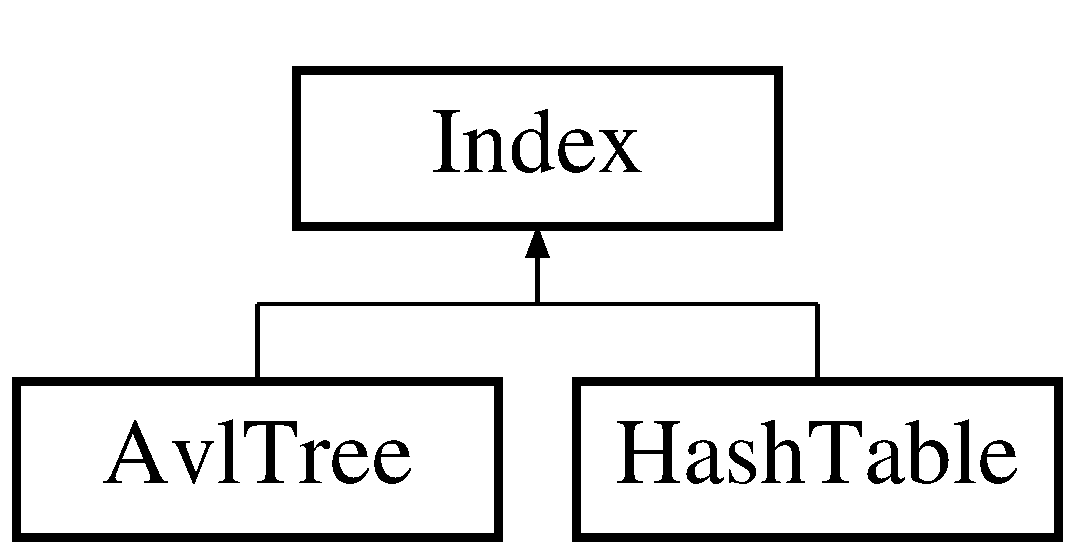
\includegraphics[height=2.000000cm]{class_index}
\end{center}
\end{figure}
\subsection*{Public Member Functions}
\begin{DoxyCompactItemize}
\item 
\hypertarget{class_index_a42835ba00eac72a146712468daaeba64}{virtual void \hyperlink{class_index_a42835ba00eac72a146712468daaeba64}{clear} ()=0}\label{class_index_a42835ba00eac72a146712468daaeba64}

\begin{DoxyCompactList}\small\item\em see documentation for A\-V\-L Tree or Hash Table \end{DoxyCompactList}\item 
\hypertarget{class_index_ad44792ad4f81ef1e17a0c6cb6f57167c}{virtual void \hyperlink{class_index_ad44792ad4f81ef1e17a0c6cb6f57167c}{insert} (string \&key, int \&pg, double \&freq, string \&header, string \&date, string \&user)=0}\label{class_index_ad44792ad4f81ef1e17a0c6cb6f57167c}

\begin{DoxyCompactList}\small\item\em see documentation for A\-V\-L Tree or Hash Table \end{DoxyCompactList}\item 
\hypertarget{class_index_a423c014174a0257d27b7e5c5834f92ed}{virtual void \hyperlink{class_index_a423c014174a0257d27b7e5c5834f92ed}{insert\-L\-L} (string \&key, \hyperlink{class_linked_list}{Linked\-List} $\ast$\&ll)=0}\label{class_index_a423c014174a0257d27b7e5c5834f92ed}

\begin{DoxyCompactList}\small\item\em see documentation for A\-V\-L Tree or Hash Table \end{DoxyCompactList}\item 
\hypertarget{class_index_a8ee654f84f96668a451afcf39fe2cc69}{virtual string \& \hyperlink{class_index_a8ee654f84f96668a451afcf39fe2cc69}{find\-Keyword} (string \&key)=0}\label{class_index_a8ee654f84f96668a451afcf39fe2cc69}

\begin{DoxyCompactList}\small\item\em see documentation for A\-V\-L Tree or Hash Table \end{DoxyCompactList}\item 
\hypertarget{class_index_a72c1cd00b6fce902a5d08e9278954913}{virtual \hyperlink{class_linked_list}{Linked\-List} $\ast$\& \hyperlink{class_index_a72c1cd00b6fce902a5d08e9278954913}{find\-Data} (string \&key)=0}\label{class_index_a72c1cd00b6fce902a5d08e9278954913}

\begin{DoxyCompactList}\small\item\em see documentation for A\-V\-L Tree or Hash Table \end{DoxyCompactList}\item 
\hypertarget{class_index_a0eccb696eb6548d60df4a4bce323191b}{virtual int \& \hyperlink{class_index_a0eccb696eb6548d60df4a4bce323191b}{get\-Size} ()=0}\label{class_index_a0eccb696eb6548d60df4a4bce323191b}

\begin{DoxyCompactList}\small\item\em see documentation for A\-V\-L Tree or Hash Table \end{DoxyCompactList}\end{DoxyCompactItemize}


\subsection{Detailed Description}
an interface used for the A\-V\-L Tree and Hash Table 

The documentation for this class was generated from the following file\-:\begin{DoxyCompactItemize}
\item 
index.\-h\end{DoxyCompactItemize}

\hypertarget{class_index_handler}{\section{Index\-Handler Class Reference}
\label{class_index_handler}\index{Index\-Handler@{Index\-Handler}}
}


Adds information from the document parser to the avl tree or hash table, searches the avl tree or hash table for query keywords from the query processor, and prints the number of words indexed.  




{\ttfamily \#include $<$indexhandler.\-h$>$}

\subsection*{Public Member Functions}
\begin{DoxyCompactItemize}
\item 
\hypertarget{class_index_handler_a27748387661142a2eb545be6f0499996}{\hyperlink{class_index_handler_a27748387661142a2eb545be6f0499996}{Index\-Handler} ()}\label{class_index_handler_a27748387661142a2eb545be6f0499996}

\begin{DoxyCompactList}\small\item\em \hyperlink{class_index_handler}{Index\-Handler} default constructor. \end{DoxyCompactList}\item 
\hypertarget{class_index_handler_ad787ca8cf83345ecfe332d2c3b8f8009}{\hyperlink{class_index_handler_ad787ca8cf83345ecfe332d2c3b8f8009}{$\sim$\-Index\-Handler} ()}\label{class_index_handler_ad787ca8cf83345ecfe332d2c3b8f8009}

\begin{DoxyCompactList}\small\item\em \hyperlink{class_index_handler}{Index\-Handler} destructor. \end{DoxyCompactList}\item 
void \hyperlink{class_index_handler_acbad99b5b0887fe776981d85529844d6}{add\-Word} (map$<$ string, int $>$ \&table, int \&pg, string \&title, string \&date, string \&user)
\begin{DoxyCompactList}\small\item\em add\-Word adds a word to the index. \end{DoxyCompactList}\item 
\hyperlink{class_index}{Index} $\ast$\& \hyperlink{class_index_handler_a0e010188cadc61017f9ada638842257f}{search\-Avl} (vector$<$ string $>$ \&search\-Words)
\begin{DoxyCompactList}\small\item\em search\-Avl searches the avl tree for the query keywords. \end{DoxyCompactList}\item 
\hyperlink{class_index}{Index} $\ast$\& \hyperlink{class_index_handler_a9549ae56231952fb0ff5883734e6f013}{search\-Hash} (vector$<$ string $>$ \&search\-Words)
\begin{DoxyCompactList}\small\item\em search\-Hash searches the hash table for the query keywords. \end{DoxyCompactList}\item 
\hypertarget{class_index_handler_a4cdb58399788cff4a00ef065b805952a}{void \hyperlink{class_index_handler_a4cdb58399788cff4a00ef065b805952a}{clear} ()}\label{class_index_handler_a4cdb58399788cff4a00ef065b805952a}

\begin{DoxyCompactList}\small\item\em clear clears the index structure. \end{DoxyCompactList}\item 
\hypertarget{class_index_handler_a287d4c40860b634cec7917c4f0ee6337}{void \hyperlink{class_index_handler_a287d4c40860b634cec7917c4f0ee6337}{print\-Size} ()}\label{class_index_handler_a287d4c40860b634cec7917c4f0ee6337}

\begin{DoxyCompactList}\small\item\em print\-Size prints the number of words indexed. \end{DoxyCompactList}\end{DoxyCompactItemize}


\subsection{Detailed Description}
Adds information from the document parser to the avl tree or hash table, searches the avl tree or hash table for query keywords from the query processor, and prints the number of words indexed. 

\subsection{Member Function Documentation}
\hypertarget{class_index_handler_acbad99b5b0887fe776981d85529844d6}{\index{Index\-Handler@{Index\-Handler}!add\-Word@{add\-Word}}
\index{add\-Word@{add\-Word}!IndexHandler@{Index\-Handler}}
\subsubsection[{add\-Word}]{\setlength{\rightskip}{0pt plus 5cm}void Index\-Handler\-::add\-Word (
\begin{DoxyParamCaption}
\item[{map$<$ string, int $>$ \&}]{table, }
\item[{int \&}]{pg, }
\item[{string \&}]{title, }
\item[{string \&}]{date, }
\item[{string \&}]{user}
\end{DoxyParamCaption}
)}}\label{class_index_handler_acbad99b5b0887fe776981d85529844d6}


add\-Word adds a word to the index. 


\begin{DoxyParams}{Parameters}
{\em table} & a map with string keys and int values containg words and their frequency from the parsed page \\
\hline
{\em pg} & an integer containing the page number parsed \\
\hline
{\em title} & a string containing the title of the parsed page \\
\hline
{\em date} & a string containing the date of the parsed page \\
\hline
{\em user} & a string containing the contributor's username of the parsed page \\
\hline
\end{DoxyParams}
\hypertarget{class_index_handler_a0e010188cadc61017f9ada638842257f}{\index{Index\-Handler@{Index\-Handler}!search\-Avl@{search\-Avl}}
\index{search\-Avl@{search\-Avl}!IndexHandler@{Index\-Handler}}
\subsubsection[{search\-Avl}]{\setlength{\rightskip}{0pt plus 5cm}{\bf Index} $\ast$\& Index\-Handler\-::search\-Avl (
\begin{DoxyParamCaption}
\item[{vector$<$ string $>$ \&}]{search\-Words}
\end{DoxyParamCaption}
)}}\label{class_index_handler_a0e010188cadc61017f9ada638842257f}


search\-Avl searches the avl tree for the query keywords. 


\begin{DoxyParams}{Parameters}
{\em search\-Words} & a vector of strings containing the query keywords \\
\hline
\end{DoxyParams}
\begin{DoxyReturn}{Returns}
a reference to an \hyperlink{class_index}{Index} pointer 
\end{DoxyReturn}
\hypertarget{class_index_handler_a9549ae56231952fb0ff5883734e6f013}{\index{Index\-Handler@{Index\-Handler}!search\-Hash@{search\-Hash}}
\index{search\-Hash@{search\-Hash}!IndexHandler@{Index\-Handler}}
\subsubsection[{search\-Hash}]{\setlength{\rightskip}{0pt plus 5cm}{\bf Index} $\ast$\& Index\-Handler\-::search\-Hash (
\begin{DoxyParamCaption}
\item[{vector$<$ string $>$ \&}]{search\-Words}
\end{DoxyParamCaption}
)}}\label{class_index_handler_a9549ae56231952fb0ff5883734e6f013}


search\-Hash searches the hash table for the query keywords. 


\begin{DoxyParams}{Parameters}
{\em search\-Words} & a vector of strings containing the query keywords \\
\hline
\end{DoxyParams}
\begin{DoxyReturn}{Returns}
a reference to an \hyperlink{class_index}{Index} pointer 
\end{DoxyReturn}


The documentation for this class was generated from the following files\-:\begin{DoxyCompactItemize}
\item 
indexhandler.\-h\item 
indexhandler.\-cpp\end{DoxyCompactItemize}

\hypertarget{classstring__util_1_1less__basic__string__compare}{\section{string\-\_\-util\-:\-:less\-\_\-basic\-\_\-string\-\_\-compare$<$ T $>$ Class Template Reference}
\label{classstring__util_1_1less__basic__string__compare}\index{string\-\_\-util\-::less\-\_\-basic\-\_\-string\-\_\-compare$<$ T $>$@{string\-\_\-util\-::less\-\_\-basic\-\_\-string\-\_\-compare$<$ T $>$}}
}
Inheritance diagram for string\-\_\-util\-:\-:less\-\_\-basic\-\_\-string\-\_\-compare$<$ T $>$\-:\begin{figure}[H]
\begin{center}
\leavevmode
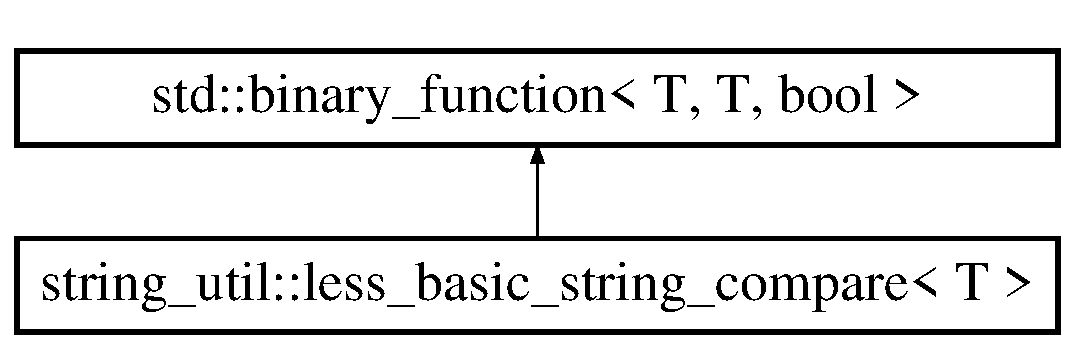
\includegraphics[height=2.000000cm]{classstring__util_1_1less__basic__string__compare}
\end{center}
\end{figure}
\subsection*{Public Member Functions}
\begin{DoxyCompactItemize}
\item 
\hypertarget{classstring__util_1_1less__basic__string__compare_a259341e58f36d8aaf75f2415de0df4d8}{bool {\bfseries operator()} (const T \&a\-\_\-, const T \&b\-\_\-) const }\label{classstring__util_1_1less__basic__string__compare_a259341e58f36d8aaf75f2415de0df4d8}

\end{DoxyCompactItemize}


The documentation for this class was generated from the following file\-:\begin{DoxyCompactItemize}
\item 
indexing/string\-\_\-util.\-h\end{DoxyCompactItemize}

\hypertarget{classstring__util_1_1less__string__compare}{\section{string\-\_\-util\-:\-:less\-\_\-string\-\_\-compare$<$ T $>$ Class Template Reference}
\label{classstring__util_1_1less__string__compare}\index{string\-\_\-util\-::less\-\_\-string\-\_\-compare$<$ T $>$@{string\-\_\-util\-::less\-\_\-string\-\_\-compare$<$ T $>$}}
}
Inheritance diagram for string\-\_\-util\-:\-:less\-\_\-string\-\_\-compare$<$ T $>$\-:\begin{figure}[H]
\begin{center}
\leavevmode
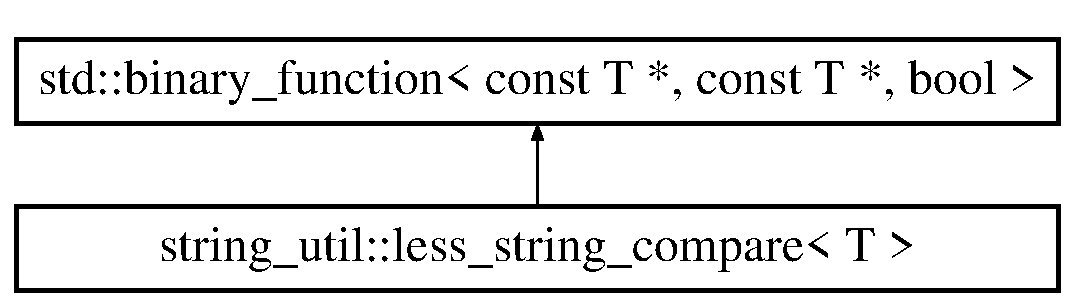
\includegraphics[height=2.000000cm]{classstring__util_1_1less__string__compare}
\end{center}
\end{figure}
\subsection*{Public Member Functions}
\begin{DoxyCompactItemize}
\item 
\hypertarget{classstring__util_1_1less__string__compare_aa97df82edd8f7e33e5715acf71759337}{bool {\bfseries operator()} (const T $\ast$a\-\_\-, const T $\ast$b\-\_\-) const }\label{classstring__util_1_1less__string__compare_aa97df82edd8f7e33e5715acf71759337}

\end{DoxyCompactItemize}


The documentation for this class was generated from the following file\-:\begin{DoxyCompactItemize}
\item 
indexing/string\-\_\-util.\-h\end{DoxyCompactItemize}

\hypertarget{classstring__util_1_1less__string__i__compare}{\section{string\-\_\-util\-:\-:less\-\_\-string\-\_\-i\-\_\-compare$<$ T $>$ Class Template Reference}
\label{classstring__util_1_1less__string__i__compare}\index{string\-\_\-util\-::less\-\_\-string\-\_\-i\-\_\-compare$<$ T $>$@{string\-\_\-util\-::less\-\_\-string\-\_\-i\-\_\-compare$<$ T $>$}}
}
Inheritance diagram for string\-\_\-util\-:\-:less\-\_\-string\-\_\-i\-\_\-compare$<$ T $>$\-:\begin{figure}[H]
\begin{center}
\leavevmode
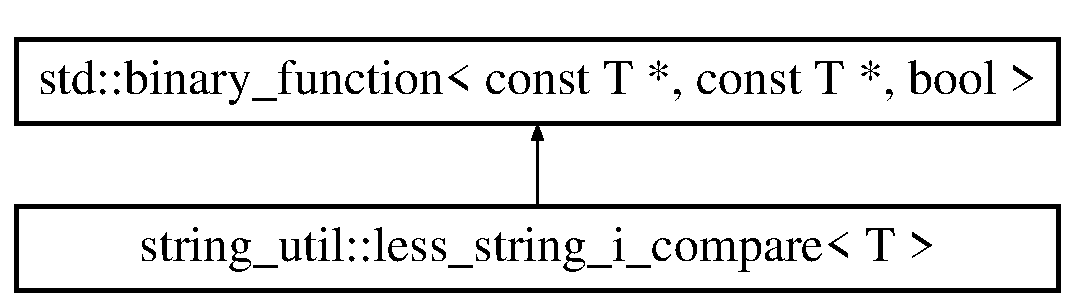
\includegraphics[height=2.000000cm]{classstring__util_1_1less__string__i__compare}
\end{center}
\end{figure}
\subsection*{Public Member Functions}
\begin{DoxyCompactItemize}
\item 
\hypertarget{classstring__util_1_1less__string__i__compare_ae2dd6a625b07bc51060805b30e7547a1}{bool {\bfseries operator()} (const T $\ast$a\-\_\-, const T $\ast$b\-\_\-) const }\label{classstring__util_1_1less__string__i__compare_ae2dd6a625b07bc51060805b30e7547a1}

\end{DoxyCompactItemize}


The documentation for this class was generated from the following file\-:\begin{DoxyCompactItemize}
\item 
indexing/string\-\_\-util.\-h\end{DoxyCompactItemize}

\hypertarget{classstring__util_1_1less__string__n__compare}{\section{string\-\_\-util\-:\-:less\-\_\-string\-\_\-n\-\_\-compare$<$ T $>$ Class Template Reference}
\label{classstring__util_1_1less__string__n__compare}\index{string\-\_\-util\-::less\-\_\-string\-\_\-n\-\_\-compare$<$ T $>$@{string\-\_\-util\-::less\-\_\-string\-\_\-n\-\_\-compare$<$ T $>$}}
}
Inheritance diagram for string\-\_\-util\-:\-:less\-\_\-string\-\_\-n\-\_\-compare$<$ T $>$\-:\begin{figure}[H]
\begin{center}
\leavevmode
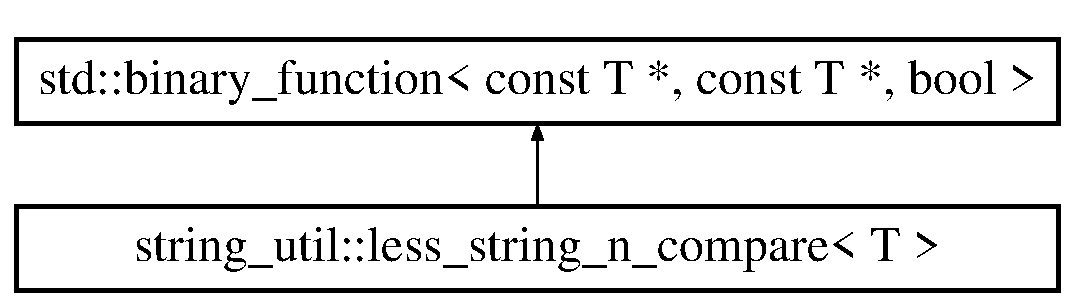
\includegraphics[height=2.000000cm]{classstring__util_1_1less__string__n__compare}
\end{center}
\end{figure}
\subsection*{Public Member Functions}
\begin{DoxyCompactItemize}
\item 
\hypertarget{classstring__util_1_1less__string__n__compare_a42b269c0aa27c5ace8b3eeb782f6d335}{{\bfseries less\-\_\-string\-\_\-n\-\_\-compare} (size\-\_\-t comparison\-\_\-size)}\label{classstring__util_1_1less__string__n__compare_a42b269c0aa27c5ace8b3eeb782f6d335}

\item 
\hypertarget{classstring__util_1_1less__string__n__compare_ab6f6bb1fbd6421cb848bba88ce18f6e0}{bool {\bfseries operator()} (const T $\ast$a\-\_\-, const T $\ast$b\-\_\-) const }\label{classstring__util_1_1less__string__n__compare_ab6f6bb1fbd6421cb848bba88ce18f6e0}

\end{DoxyCompactItemize}


The documentation for this class was generated from the following file\-:\begin{DoxyCompactItemize}
\item 
indexing/string\-\_\-util.\-h\end{DoxyCompactItemize}

\hypertarget{classstring__util_1_1less__string__natural__order__i__compare}{\section{string\-\_\-util\-:\-:less\-\_\-string\-\_\-natural\-\_\-order\-\_\-i\-\_\-compare$<$ T $>$ Class Template Reference}
\label{classstring__util_1_1less__string__natural__order__i__compare}\index{string\-\_\-util\-::less\-\_\-string\-\_\-natural\-\_\-order\-\_\-i\-\_\-compare$<$ T $>$@{string\-\_\-util\-::less\-\_\-string\-\_\-natural\-\_\-order\-\_\-i\-\_\-compare$<$ T $>$}}
}
Inheritance diagram for string\-\_\-util\-:\-:less\-\_\-string\-\_\-natural\-\_\-order\-\_\-i\-\_\-compare$<$ T $>$\-:\begin{figure}[H]
\begin{center}
\leavevmode
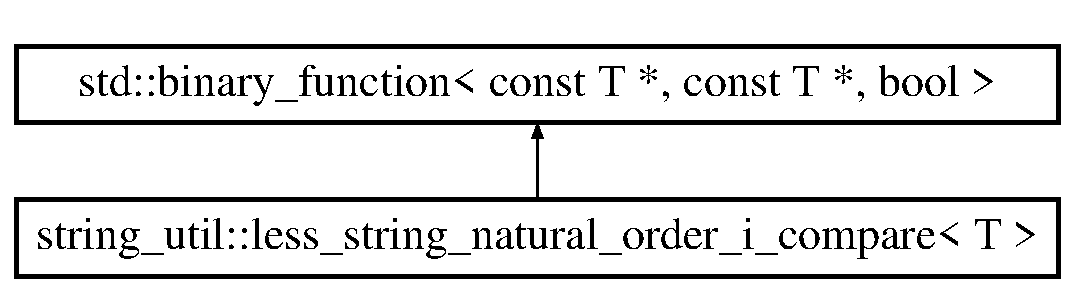
\includegraphics[height=2.000000cm]{classstring__util_1_1less__string__natural__order__i__compare}
\end{center}
\end{figure}
\subsection*{Public Member Functions}
\begin{DoxyCompactItemize}
\item 
\hypertarget{classstring__util_1_1less__string__natural__order__i__compare_a213ba84bcb81fa025951194acbdb899c}{bool {\bfseries operator()} (const T $\ast$a\-\_\-, const T $\ast$b\-\_\-) const }\label{classstring__util_1_1less__string__natural__order__i__compare_a213ba84bcb81fa025951194acbdb899c}

\end{DoxyCompactItemize}


The documentation for this class was generated from the following file\-:\begin{DoxyCompactItemize}
\item 
indexing/string\-\_\-util.\-h\end{DoxyCompactItemize}

\hypertarget{classstring__util_1_1less__string__ni__compare}{\section{string\-\_\-util\-:\-:less\-\_\-string\-\_\-ni\-\_\-compare$<$ T $>$ Class Template Reference}
\label{classstring__util_1_1less__string__ni__compare}\index{string\-\_\-util\-::less\-\_\-string\-\_\-ni\-\_\-compare$<$ T $>$@{string\-\_\-util\-::less\-\_\-string\-\_\-ni\-\_\-compare$<$ T $>$}}
}
Inheritance diagram for string\-\_\-util\-:\-:less\-\_\-string\-\_\-ni\-\_\-compare$<$ T $>$\-:\begin{figure}[H]
\begin{center}
\leavevmode
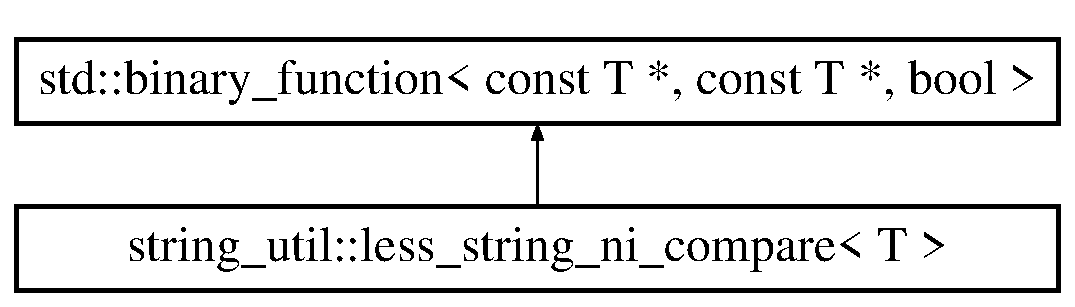
\includegraphics[height=2.000000cm]{classstring__util_1_1less__string__ni__compare}
\end{center}
\end{figure}
\subsection*{Public Member Functions}
\begin{DoxyCompactItemize}
\item 
\hypertarget{classstring__util_1_1less__string__ni__compare_aec49bc79089ab2e54ff4752bbbabe6bf}{{\bfseries less\-\_\-string\-\_\-ni\-\_\-compare} (size\-\_\-t comparison\-\_\-size)}\label{classstring__util_1_1less__string__ni__compare_aec49bc79089ab2e54ff4752bbbabe6bf}

\item 
\hypertarget{classstring__util_1_1less__string__ni__compare_a6050f7d7b4998343cc5c46dca8b28bcc}{bool {\bfseries operator()} (const T $\ast$a\-\_\-, const T $\ast$b\-\_\-) const }\label{classstring__util_1_1less__string__ni__compare_a6050f7d7b4998343cc5c46dca8b28bcc}

\end{DoxyCompactItemize}


The documentation for this class was generated from the following file\-:\begin{DoxyCompactItemize}
\item 
indexing/string\-\_\-util.\-h\end{DoxyCompactItemize}

\hypertarget{class_linked_list}{\section{Linked\-List Class Reference}
\label{class_linked_list}\index{Linked\-List@{Linked\-List}}
}
\subsection*{Public Member Functions}
\begin{DoxyCompactItemize}
\item 
\hypertarget{class_linked_list_afe7f78983e173f8018927cf2ad11a5aa}{\hyperlink{class_linked_list_afe7f78983e173f8018927cf2ad11a5aa}{Linked\-List} ()}\label{class_linked_list_afe7f78983e173f8018927cf2ad11a5aa}

\begin{DoxyCompactList}\small\item\em \hyperlink{class_linked_list}{Linked\-List} default constructor. \end{DoxyCompactList}\item 
\hypertarget{class_linked_list_a35811ed58ff0d8d9cc9b309b8d8f5111}{\hyperlink{class_linked_list_a35811ed58ff0d8d9cc9b309b8d8f5111}{$\sim$\-Linked\-List} ()}\label{class_linked_list_a35811ed58ff0d8d9cc9b309b8d8f5111}

\begin{DoxyCompactList}\small\item\em \hyperlink{class_linked_list}{Linked\-List} destructor. \end{DoxyCompactList}\item 
\hyperlink{class_linked_list_ab34de0df2c51416dc15596f45809842b}{Linked\-List} (const \hyperlink{class_linked_list}{Linked\-List} \&cp)
\begin{DoxyCompactList}\small\item\em \hyperlink{class_linked_list}{Linked\-List} copy constructor. \end{DoxyCompactList}\item 
\hypertarget{class_linked_list_a261977565e78dd74f288d47ba5865242}{void \hyperlink{class_linked_list_a261977565e78dd74f288d47ba5865242}{clear} ()}\label{class_linked_list_a261977565e78dd74f288d47ba5865242}

\begin{DoxyCompactList}\small\item\em clear clears the linked list. \end{DoxyCompactList}\item 
\hyperlink{class_linked_list}{Linked\-List} \& \hyperlink{class_linked_list_a522a87f8da5057b0e0bb4565bb348ec3}{operator=} (const \hyperlink{class_linked_list}{Linked\-List} \&cp)
\begin{DoxyCompactList}\small\item\em overloaded assignment operator \end{DoxyCompactList}\item 
bool \hyperlink{class_linked_list_a22987b83cc33313bb594a2d67aa9f289}{empty} ()
\begin{DoxyCompactList}\small\item\em empty checks if the linked list is empty. \end{DoxyCompactList}\item 
void \hyperlink{class_linked_list_abf524a3e1cd90e8374fa5c24f64dfd18}{push\-\_\-back} (int pg, double freq, string doc\-Name, string date\-Made, string user\-Name)
\begin{DoxyCompactList}\small\item\em push\-\_\-back adds a node to the end of the linked list. \end{DoxyCompactList}\item 
int \& \hyperlink{class_linked_list_a0428164a801662e4908f87ce826cedbf}{get\-Page\-Number} (int index)
\begin{DoxyCompactList}\small\item\em get\-Page\-Number gets the page number from a node in the linked list. \end{DoxyCompactList}\item 
double \& \hyperlink{class_linked_list_a36b29b42c7e4316a4a1663cbc60804a7}{get\-Frequency} (int index)
\begin{DoxyCompactList}\small\item\em get\-Frequency gets the term frequency from a node in the linked list. \end{DoxyCompactList}\item 
string \& \hyperlink{class_linked_list_ab1605d5e12f51dd7f00d042415b80232}{get\-Title} (int index)
\begin{DoxyCompactList}\small\item\em get\-Title gets the page title from a node in the linked list. \end{DoxyCompactList}\item 
string \& \hyperlink{class_linked_list_a49761c9b8dd1dc1df7a56b0a3536a15d}{get\-Date} (int index)
\begin{DoxyCompactList}\small\item\em get\-Date gets the page date from a node in the linked list. \end{DoxyCompactList}\item 
string \& \hyperlink{class_linked_list_ad88d540fff6aea9502372fc21035e404}{get\-User} (int index)
\begin{DoxyCompactList}\small\item\em get\-User gets the contributor's username from a node in the linked list. \end{DoxyCompactList}\item 
void \hyperlink{class_linked_list_a7bfa0c7ef3608c772d8837226fa0baca}{set\-\_\-at} (int index, double freq)
\begin{DoxyCompactList}\small\item\em set\-\_\-at updates the frequency of a word at a specified node. \end{DoxyCompactList}\item 
void \hyperlink{class_linked_list_a1d13e00736ede314d40f26a64769cc35}{set\-\_\-at} (int index, int pg, double freq, string doc\-Name, string date\-Made, string user\-Name)
\begin{DoxyCompactList}\small\item\em set\-\_\-at updates the page number, frequency, page title, page date, and contributor's username at a specified index. \end{DoxyCompactList}\item 
void \hyperlink{class_linked_list_aed2890ca9479d953248e024babee04f3}{find\-Set} (int pg, double freq)
\begin{DoxyCompactList}\small\item\em find\-Set updates the word frequency for the page \end{DoxyCompactList}\item 
void \hyperlink{class_linked_list_a3429db79356a0203d8c50057cb76a03b}{delete\-At} (int index)
\begin{DoxyCompactList}\small\item\em delete\-At deletes a specified node in the linked list. \end{DoxyCompactList}\item 
int \hyperlink{class_linked_list_a4224bd8bf5f18b7b6f9fa66ee2c35702}{size} ()
\begin{DoxyCompactList}\small\item\em size gets the size of the linked list. \end{DoxyCompactList}\item 
\hypertarget{class_linked_list_ad6fdfc5ff2d9b4209ac3104402676574}{void \hyperlink{class_linked_list_ad6fdfc5ff2d9b4209ac3104402676574}{sort} (int start, int end)}\label{class_linked_list_ad6fdfc5ff2d9b4209ac3104402676574}

\begin{DoxyCompactList}\small\item\em sort sorts the linked list by term frequency in descending order. \end{DoxyCompactList}\item 
int \hyperlink{class_linked_list_aabad92ed4258e22f8f25ef4db83ace63}{partition} (int low, int high)
\begin{DoxyCompactList}\small\item\em partition recursive function that sorts the linked list. \end{DoxyCompactList}\item 
void \hyperlink{class_linked_list_a6328a045297f16d1ae2f3964126f1d3e}{swap} (int a, int b)
\begin{DoxyCompactList}\small\item\em swap swaps the contents of a node in the linked list. \end{DoxyCompactList}\item 
bool \hyperlink{class_linked_list_a9ccb3e8a33f1f6a12884782b93a837ae}{contains} (int \&pg)
\begin{DoxyCompactList}\small\item\em contains checks if the linked list contains a page number \end{DoxyCompactList}\item 
int \hyperlink{class_linked_list_ae43a82e40aaf7709c34cf989a2905750}{find\-Iterator} (int \&pg)
\begin{DoxyCompactList}\small\item\em find\-Iterator returns an integer representing the index number of a node containing a specific page number. \end{DoxyCompactList}\item 
void \hyperlink{class_linked_list_a420d35a949ef7acbb5cd13a2900fe813}{output} ()
\begin{DoxyCompactList}\small\item\em output prints the contents of the nodes in the linked list for the first 15 nodes and the number of nodes for the particular word searched for. \end{DoxyCompactList}\end{DoxyCompactItemize}


\subsection{Constructor \& Destructor Documentation}
\hypertarget{class_linked_list_ab34de0df2c51416dc15596f45809842b}{\index{Linked\-List@{Linked\-List}!Linked\-List@{Linked\-List}}
\index{Linked\-List@{Linked\-List}!LinkedList@{Linked\-List}}
\subsubsection[{Linked\-List}]{\setlength{\rightskip}{0pt plus 5cm}Linked\-List\-::\-Linked\-List (
\begin{DoxyParamCaption}
\item[{const {\bf Linked\-List} \&}]{cp}
\end{DoxyParamCaption}
)\hspace{0.3cm}{\ttfamily [inline]}}}\label{class_linked_list_ab34de0df2c51416dc15596f45809842b}


\hyperlink{class_linked_list}{Linked\-List} copy constructor. 


\begin{DoxyParams}{Parameters}
{\em cp} & a constant \hyperlink{class_linked_list}{Linked\-List} object \\
\hline
\end{DoxyParams}


\subsection{Member Function Documentation}
\hypertarget{class_linked_list_a9ccb3e8a33f1f6a12884782b93a837ae}{\index{Linked\-List@{Linked\-List}!contains@{contains}}
\index{contains@{contains}!LinkedList@{Linked\-List}}
\subsubsection[{contains}]{\setlength{\rightskip}{0pt plus 5cm}bool Linked\-List\-::contains (
\begin{DoxyParamCaption}
\item[{int \&}]{pg}
\end{DoxyParamCaption}
)\hspace{0.3cm}{\ttfamily [inline]}}}\label{class_linked_list_a9ccb3e8a33f1f6a12884782b93a837ae}


contains checks if the linked list contains a page number 


\begin{DoxyParams}{Parameters}
{\em pg} & an integer containing a page number \\
\hline
\end{DoxyParams}
\begin{DoxyReturn}{Returns}
true if the page is in the linked list, false if it isn't 
\end{DoxyReturn}
\hypertarget{class_linked_list_a3429db79356a0203d8c50057cb76a03b}{\index{Linked\-List@{Linked\-List}!delete\-At@{delete\-At}}
\index{delete\-At@{delete\-At}!LinkedList@{Linked\-List}}
\subsubsection[{delete\-At}]{\setlength{\rightskip}{0pt plus 5cm}void Linked\-List\-::delete\-At (
\begin{DoxyParamCaption}
\item[{int}]{index}
\end{DoxyParamCaption}
)\hspace{0.3cm}{\ttfamily [inline]}}}\label{class_linked_list_a3429db79356a0203d8c50057cb76a03b}


delete\-At deletes a specified node in the linked list. 


\begin{DoxyParams}{Parameters}
{\em index} & index an integer representing the node number in the linked list \\
\hline
\end{DoxyParams}
\hypertarget{class_linked_list_a22987b83cc33313bb594a2d67aa9f289}{\index{Linked\-List@{Linked\-List}!empty@{empty}}
\index{empty@{empty}!LinkedList@{Linked\-List}}
\subsubsection[{empty}]{\setlength{\rightskip}{0pt plus 5cm}bool Linked\-List\-::empty (
\begin{DoxyParamCaption}
{}
\end{DoxyParamCaption}
)\hspace{0.3cm}{\ttfamily [inline]}}}\label{class_linked_list_a22987b83cc33313bb594a2d67aa9f289}


empty checks if the linked list is empty. 

\begin{DoxyReturn}{Returns}
true if the linked list is empty and false if it is not empty 
\end{DoxyReturn}
\hypertarget{class_linked_list_ae43a82e40aaf7709c34cf989a2905750}{\index{Linked\-List@{Linked\-List}!find\-Iterator@{find\-Iterator}}
\index{find\-Iterator@{find\-Iterator}!LinkedList@{Linked\-List}}
\subsubsection[{find\-Iterator}]{\setlength{\rightskip}{0pt plus 5cm}int Linked\-List\-::find\-Iterator (
\begin{DoxyParamCaption}
\item[{int \&}]{pg}
\end{DoxyParamCaption}
)\hspace{0.3cm}{\ttfamily [inline]}}}\label{class_linked_list_ae43a82e40aaf7709c34cf989a2905750}


find\-Iterator returns an integer representing the index number of a node containing a specific page number. 


\begin{DoxyParams}{Parameters}
{\em pg} & an integer containing a page number \\
\hline
\end{DoxyParams}
\begin{DoxyReturn}{Returns}

\end{DoxyReturn}
\hypertarget{class_linked_list_aed2890ca9479d953248e024babee04f3}{\index{Linked\-List@{Linked\-List}!find\-Set@{find\-Set}}
\index{find\-Set@{find\-Set}!LinkedList@{Linked\-List}}
\subsubsection[{find\-Set}]{\setlength{\rightskip}{0pt plus 5cm}void Linked\-List\-::find\-Set (
\begin{DoxyParamCaption}
\item[{int}]{pg, }
\item[{double}]{freq}
\end{DoxyParamCaption}
)\hspace{0.3cm}{\ttfamily [inline]}}}\label{class_linked_list_aed2890ca9479d953248e024babee04f3}


find\-Set updates the word frequency for the page 


\begin{DoxyParams}{Parameters}
{\em pg} & an integer containing a page number \\
\hline
{\em freq} & an integer containing the word frequency \\
\hline
\end{DoxyParams}
\hypertarget{class_linked_list_a49761c9b8dd1dc1df7a56b0a3536a15d}{\index{Linked\-List@{Linked\-List}!get\-Date@{get\-Date}}
\index{get\-Date@{get\-Date}!LinkedList@{Linked\-List}}
\subsubsection[{get\-Date}]{\setlength{\rightskip}{0pt plus 5cm}string\& Linked\-List\-::get\-Date (
\begin{DoxyParamCaption}
\item[{int}]{index}
\end{DoxyParamCaption}
)\hspace{0.3cm}{\ttfamily [inline]}}}\label{class_linked_list_a49761c9b8dd1dc1df7a56b0a3536a15d}


get\-Date gets the page date from a node in the linked list. 


\begin{DoxyParams}{Parameters}
{\em index} & an integer representing the node number in the linked list \\
\hline
\end{DoxyParams}
\begin{DoxyReturn}{Returns}
a string representing the page date from the specified node 
\end{DoxyReturn}
\hypertarget{class_linked_list_a36b29b42c7e4316a4a1663cbc60804a7}{\index{Linked\-List@{Linked\-List}!get\-Frequency@{get\-Frequency}}
\index{get\-Frequency@{get\-Frequency}!LinkedList@{Linked\-List}}
\subsubsection[{get\-Frequency}]{\setlength{\rightskip}{0pt plus 5cm}double\& Linked\-List\-::get\-Frequency (
\begin{DoxyParamCaption}
\item[{int}]{index}
\end{DoxyParamCaption}
)\hspace{0.3cm}{\ttfamily [inline]}}}\label{class_linked_list_a36b29b42c7e4316a4a1663cbc60804a7}


get\-Frequency gets the term frequency from a node in the linked list. 


\begin{DoxyParams}{Parameters}
{\em index} & an integer representing the node number in the linked list \\
\hline
\end{DoxyParams}
\begin{DoxyReturn}{Returns}
a double representing the term frequency from the specified node 
\end{DoxyReturn}
\hypertarget{class_linked_list_a0428164a801662e4908f87ce826cedbf}{\index{Linked\-List@{Linked\-List}!get\-Page\-Number@{get\-Page\-Number}}
\index{get\-Page\-Number@{get\-Page\-Number}!LinkedList@{Linked\-List}}
\subsubsection[{get\-Page\-Number}]{\setlength{\rightskip}{0pt plus 5cm}int\& Linked\-List\-::get\-Page\-Number (
\begin{DoxyParamCaption}
\item[{int}]{index}
\end{DoxyParamCaption}
)\hspace{0.3cm}{\ttfamily [inline]}}}\label{class_linked_list_a0428164a801662e4908f87ce826cedbf}


get\-Page\-Number gets the page number from a node in the linked list. 


\begin{DoxyParams}{Parameters}
{\em index} & an integer representing the node number in the linked list \\
\hline
\end{DoxyParams}
\begin{DoxyReturn}{Returns}
an integer representing the page number from the specified node 
\end{DoxyReturn}
\hypertarget{class_linked_list_ab1605d5e12f51dd7f00d042415b80232}{\index{Linked\-List@{Linked\-List}!get\-Title@{get\-Title}}
\index{get\-Title@{get\-Title}!LinkedList@{Linked\-List}}
\subsubsection[{get\-Title}]{\setlength{\rightskip}{0pt plus 5cm}string\& Linked\-List\-::get\-Title (
\begin{DoxyParamCaption}
\item[{int}]{index}
\end{DoxyParamCaption}
)\hspace{0.3cm}{\ttfamily [inline]}}}\label{class_linked_list_ab1605d5e12f51dd7f00d042415b80232}


get\-Title gets the page title from a node in the linked list. 


\begin{DoxyParams}{Parameters}
{\em index} & an integer representing the node number in the linked list \\
\hline
\end{DoxyParams}
\begin{DoxyReturn}{Returns}
a string representing the page title from the specified node 
\end{DoxyReturn}
\hypertarget{class_linked_list_ad88d540fff6aea9502372fc21035e404}{\index{Linked\-List@{Linked\-List}!get\-User@{get\-User}}
\index{get\-User@{get\-User}!LinkedList@{Linked\-List}}
\subsubsection[{get\-User}]{\setlength{\rightskip}{0pt plus 5cm}string\& Linked\-List\-::get\-User (
\begin{DoxyParamCaption}
\item[{int}]{index}
\end{DoxyParamCaption}
)\hspace{0.3cm}{\ttfamily [inline]}}}\label{class_linked_list_ad88d540fff6aea9502372fc21035e404}


get\-User gets the contributor's username from a node in the linked list. 


\begin{DoxyParams}{Parameters}
{\em index} & an integer representing the node number in the linked list \\
\hline
\end{DoxyParams}
\begin{DoxyReturn}{Returns}
a string representing the contributor's username from the specified node. 
\end{DoxyReturn}
\hypertarget{class_linked_list_a522a87f8da5057b0e0bb4565bb348ec3}{\index{Linked\-List@{Linked\-List}!operator=@{operator=}}
\index{operator=@{operator=}!LinkedList@{Linked\-List}}
\subsubsection[{operator=}]{\setlength{\rightskip}{0pt plus 5cm}{\bf Linked\-List}\& Linked\-List\-::operator= (
\begin{DoxyParamCaption}
\item[{const {\bf Linked\-List} \&}]{cp}
\end{DoxyParamCaption}
)\hspace{0.3cm}{\ttfamily [inline]}}}\label{class_linked_list_a522a87f8da5057b0e0bb4565bb348ec3}


overloaded assignment operator 


\begin{DoxyParams}{Parameters}
{\em cp} & a constant \hyperlink{class_linked_list}{Linked\-List} object \\
\hline
\end{DoxyParams}
\begin{DoxyReturn}{Returns}
a \hyperlink{class_linked_list}{Linked\-List} object 
\end{DoxyReturn}
\hypertarget{class_linked_list_a420d35a949ef7acbb5cd13a2900fe813}{\index{Linked\-List@{Linked\-List}!output@{output}}
\index{output@{output}!LinkedList@{Linked\-List}}
\subsubsection[{output}]{\setlength{\rightskip}{0pt plus 5cm}void Linked\-List\-::output (
\begin{DoxyParamCaption}
{}
\end{DoxyParamCaption}
)\hspace{0.3cm}{\ttfamily [inline]}}}\label{class_linked_list_a420d35a949ef7acbb5cd13a2900fe813}


output prints the contents of the nodes in the linked list for the first 15 nodes and the number of nodes for the particular word searched for. 

Prints 15 because the output only requires 15 pages to be printed. \hypertarget{class_linked_list_aabad92ed4258e22f8f25ef4db83ace63}{\index{Linked\-List@{Linked\-List}!partition@{partition}}
\index{partition@{partition}!LinkedList@{Linked\-List}}
\subsubsection[{partition}]{\setlength{\rightskip}{0pt plus 5cm}int Linked\-List\-::partition (
\begin{DoxyParamCaption}
\item[{int}]{low, }
\item[{int}]{high}
\end{DoxyParamCaption}
)\hspace{0.3cm}{\ttfamily [inline]}}}\label{class_linked_list_aabad92ed4258e22f8f25ef4db83ace63}


partition recursive function that sorts the linked list. 


\begin{DoxyParams}{Parameters}
{\em low} & an integer containing the size of first half of the linked list \\
\hline
{\em high} & an integer containing the size of the second half of the linked list \\
\hline
\end{DoxyParams}
\begin{DoxyReturn}{Returns}

\end{DoxyReturn}
\hypertarget{class_linked_list_abf524a3e1cd90e8374fa5c24f64dfd18}{\index{Linked\-List@{Linked\-List}!push\-\_\-back@{push\-\_\-back}}
\index{push\-\_\-back@{push\-\_\-back}!LinkedList@{Linked\-List}}
\subsubsection[{push\-\_\-back}]{\setlength{\rightskip}{0pt plus 5cm}void Linked\-List\-::push\-\_\-back (
\begin{DoxyParamCaption}
\item[{int}]{pg, }
\item[{double}]{freq, }
\item[{string}]{doc\-Name, }
\item[{string}]{date\-Made, }
\item[{string}]{user\-Name}
\end{DoxyParamCaption}
)\hspace{0.3cm}{\ttfamily [inline]}}}\label{class_linked_list_abf524a3e1cd90e8374fa5c24f64dfd18}


push\-\_\-back adds a node to the end of the linked list. 


\begin{DoxyParams}{Parameters}
{\em pg} & an integer containing the page number in the xml file \\
\hline
{\em freq} & a double containing the term frequency for the document \\
\hline
{\em doc\-Name} & a string containing the title of the page \\
\hline
{\em date\-Made} & a string containing the timestamp of the page \\
\hline
{\em user\-Name} & a string containing the page contributor's username \\
\hline
\end{DoxyParams}
\hypertarget{class_linked_list_a7bfa0c7ef3608c772d8837226fa0baca}{\index{Linked\-List@{Linked\-List}!set\-\_\-at@{set\-\_\-at}}
\index{set\-\_\-at@{set\-\_\-at}!LinkedList@{Linked\-List}}
\subsubsection[{set\-\_\-at}]{\setlength{\rightskip}{0pt plus 5cm}void Linked\-List\-::set\-\_\-at (
\begin{DoxyParamCaption}
\item[{int}]{index, }
\item[{double}]{freq}
\end{DoxyParamCaption}
)\hspace{0.3cm}{\ttfamily [inline]}}}\label{class_linked_list_a7bfa0c7ef3608c772d8837226fa0baca}


set\-\_\-at updates the frequency of a word at a specified node. 


\begin{DoxyParams}{Parameters}
{\em index} & an integer containing an index number \\
\hline
{\em freq} & a double containing the word frequency \\
\hline
\end{DoxyParams}
\hypertarget{class_linked_list_a1d13e00736ede314d40f26a64769cc35}{\index{Linked\-List@{Linked\-List}!set\-\_\-at@{set\-\_\-at}}
\index{set\-\_\-at@{set\-\_\-at}!LinkedList@{Linked\-List}}
\subsubsection[{set\-\_\-at}]{\setlength{\rightskip}{0pt plus 5cm}void Linked\-List\-::set\-\_\-at (
\begin{DoxyParamCaption}
\item[{int}]{index, }
\item[{int}]{pg, }
\item[{double}]{freq, }
\item[{string}]{doc\-Name, }
\item[{string}]{date\-Made, }
\item[{string}]{user\-Name}
\end{DoxyParamCaption}
)\hspace{0.3cm}{\ttfamily [inline]}}}\label{class_linked_list_a1d13e00736ede314d40f26a64769cc35}


set\-\_\-at updates the page number, frequency, page title, page date, and contributor's username at a specified index. 


\begin{DoxyParams}{Parameters}
{\em index} & an integer containing an index number \\
\hline
{\em pg} & an integer containing the page number \\
\hline
{\em freq} & a double containing the word frequency \\
\hline
{\em doc\-Name} & a string containing the page title \\
\hline
{\em date\-Made} & a string containing the page date \\
\hline
{\em user\-Name} & a string containing the page contributor's username \\
\hline
\end{DoxyParams}
\hypertarget{class_linked_list_a4224bd8bf5f18b7b6f9fa66ee2c35702}{\index{Linked\-List@{Linked\-List}!size@{size}}
\index{size@{size}!LinkedList@{Linked\-List}}
\subsubsection[{size}]{\setlength{\rightskip}{0pt plus 5cm}int Linked\-List\-::size (
\begin{DoxyParamCaption}
{}
\end{DoxyParamCaption}
)\hspace{0.3cm}{\ttfamily [inline]}}}\label{class_linked_list_a4224bd8bf5f18b7b6f9fa66ee2c35702}


size gets the size of the linked list. 

\begin{DoxyReturn}{Returns}
an integer representing the size of the linked list 
\end{DoxyReturn}
\hypertarget{class_linked_list_a6328a045297f16d1ae2f3964126f1d3e}{\index{Linked\-List@{Linked\-List}!swap@{swap}}
\index{swap@{swap}!LinkedList@{Linked\-List}}
\subsubsection[{swap}]{\setlength{\rightskip}{0pt plus 5cm}void Linked\-List\-::swap (
\begin{DoxyParamCaption}
\item[{int}]{a, }
\item[{int}]{b}
\end{DoxyParamCaption}
)\hspace{0.3cm}{\ttfamily [inline]}}}\label{class_linked_list_a6328a045297f16d1ae2f3964126f1d3e}


swap swaps the contents of a node in the linked list. 


\begin{DoxyParams}{Parameters}
{\em a} & an integer containing a node number in the linked list \\
\hline
{\em b} & an integer containing a node number in the linked list \\
\hline
\end{DoxyParams}


The documentation for this class was generated from the following file\-:\begin{DoxyCompactItemize}
\item 
linkedlist.\-h\end{DoxyCompactItemize}

\hypertarget{classrapidxml_1_1memory__pool}{\section{rapidxml\-:\-:memory\-\_\-pool$<$ Ch $>$ Class Template Reference}
\label{classrapidxml_1_1memory__pool}\index{rapidxml\-::memory\-\_\-pool$<$ Ch $>$@{rapidxml\-::memory\-\_\-pool$<$ Ch $>$}}
}


{\ttfamily \#include $<$rapidxml.\-hpp$>$}

Inheritance diagram for rapidxml\-:\-:memory\-\_\-pool$<$ Ch $>$\-:\begin{figure}[H]
\begin{center}
\leavevmode
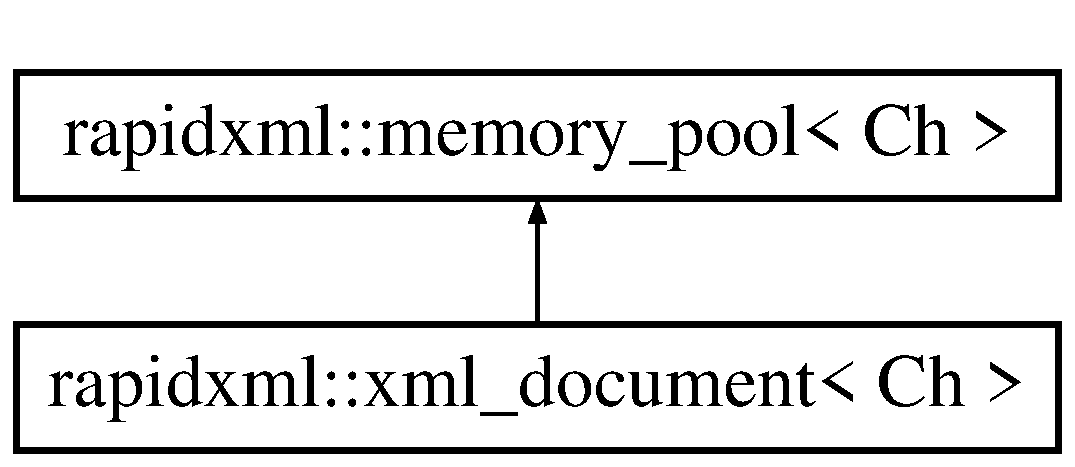
\includegraphics[height=2.000000cm]{classrapidxml_1_1memory__pool}
\end{center}
\end{figure}
\subsection*{Public Member Functions}
\begin{DoxyCompactItemize}
\item 
\hypertarget{classrapidxml_1_1memory__pool_a0b609da81dff28a19ebd704400788429}{\hyperlink{classrapidxml_1_1memory__pool_a0b609da81dff28a19ebd704400788429}{memory\-\_\-pool} ()}\label{classrapidxml_1_1memory__pool_a0b609da81dff28a19ebd704400788429}

\begin{DoxyCompactList}\small\item\em Constructs empty pool with default allocator functions. \end{DoxyCompactList}\item 
\hyperlink{classrapidxml_1_1memory__pool_a0a3e82126e59e4077f41e933130bb5a0}{$\sim$memory\-\_\-pool} ()
\item 
\hyperlink{classrapidxml_1_1xml__node}{xml\-\_\-node}$<$ Ch $>$ $\ast$ \hyperlink{classrapidxml_1_1memory__pool_a4118581c29ee9a2f6b55ebf7dac185f8}{allocate\-\_\-node} (node\-\_\-type type, const Ch $\ast$name=0, const Ch $\ast$value=0, std\-::size\-\_\-t name\-\_\-size=0, std\-::size\-\_\-t value\-\_\-size=0)
\item 
\hyperlink{classrapidxml_1_1xml__attribute}{xml\-\_\-attribute}$<$ Ch $>$ $\ast$ \hyperlink{classrapidxml_1_1memory__pool_a3de2a66c983336e006ea3844e244ed30}{allocate\-\_\-attribute} (const Ch $\ast$name=0, const Ch $\ast$value=0, std\-::size\-\_\-t name\-\_\-size=0, std\-::size\-\_\-t value\-\_\-size=0)
\item 
Ch $\ast$ \hyperlink{classrapidxml_1_1memory__pool_a171941b39d55b868358da97462185f58}{allocate\-\_\-string} (const Ch $\ast$source=0, std\-::size\-\_\-t size=0)
\item 
\hyperlink{classrapidxml_1_1xml__node}{xml\-\_\-node}$<$ Ch $>$ $\ast$ \hyperlink{classrapidxml_1_1memory__pool_a0a10679fc17597d339a0dc107f8a94ac}{clone\-\_\-node} (const \hyperlink{classrapidxml_1_1xml__node}{xml\-\_\-node}$<$ Ch $>$ $\ast$source, \hyperlink{classrapidxml_1_1xml__node}{xml\-\_\-node}$<$ Ch $>$ $\ast$result=0)
\item 
void \hyperlink{classrapidxml_1_1memory__pool_aad377c835fdaed1cb2cc9df194cf84e4}{clear} ()
\item 
void \hyperlink{classrapidxml_1_1memory__pool_a84d3d8d2cdfc00501e1dcf26d889ae03}{set\-\_\-allocator} (alloc\-\_\-func $\ast$af, free\-\_\-func $\ast$ff)
\end{DoxyCompactItemize}


\subsection{Detailed Description}
\subsubsection*{template$<$class Ch = char$>$class rapidxml\-::memory\-\_\-pool$<$ Ch $>$}

This class is used by the parser to create new nodes and attributes, without overheads of dynamic memory allocation. In most cases, you will not need to use this class directly. However, if you need to create nodes manually or modify names/values of nodes, you are encouraged to use \hyperlink{classrapidxml_1_1memory__pool}{memory\-\_\-pool} of relevant \hyperlink{classrapidxml_1_1xml__document}{xml\-\_\-document} to allocate the memory. Not only is this faster than allocating them by using {\ttfamily new} operator, but also their lifetime will be tied to the lifetime of document, possibly simplyfing memory management. \par
\par
 Call \hyperlink{classrapidxml_1_1memory__pool_a4118581c29ee9a2f6b55ebf7dac185f8}{allocate\-\_\-node()} or \hyperlink{classrapidxml_1_1memory__pool_a3de2a66c983336e006ea3844e244ed30}{allocate\-\_\-attribute()} functions to obtain new nodes or attributes from the pool. You can also call \hyperlink{classrapidxml_1_1memory__pool_a171941b39d55b868358da97462185f58}{allocate\-\_\-string()} function to allocate strings. Such strings can then be used as names or values of nodes without worrying about their lifetime. Note that there is no {\ttfamily free()} function -- all allocations are freed at once when \hyperlink{classrapidxml_1_1memory__pool_aad377c835fdaed1cb2cc9df194cf84e4}{clear()} function is called, or when the pool is destroyed. \par
\par
 It is also possible to create a standalone \hyperlink{classrapidxml_1_1memory__pool}{memory\-\_\-pool}, and use it to allocate nodes, whose lifetime will not be tied to any document. \par
\par
 Pool maintains {\ttfamily R\-A\-P\-I\-D\-X\-M\-L\-\_\-\-S\-T\-A\-T\-I\-C\-\_\-\-P\-O\-O\-L\-\_\-\-S\-I\-Z\-E} bytes of statically allocated memory. Until static memory is exhausted, no dynamic memory allocations are done. When static memory is exhausted, pool allocates additional blocks of memory of size {\ttfamily R\-A\-P\-I\-D\-X\-M\-L\-\_\-\-D\-Y\-N\-A\-M\-I\-C\-\_\-\-P\-O\-O\-L\-\_\-\-S\-I\-Z\-E} each, by using global {\ttfamily new\mbox{[}\mbox{]}} and {\ttfamily delete\mbox{[}\mbox{]}} operators. This behaviour can be changed by setting custom allocation routines. Use \hyperlink{classrapidxml_1_1memory__pool_a84d3d8d2cdfc00501e1dcf26d889ae03}{set\-\_\-allocator()} function to set them. \par
\par
 Allocations for nodes, attributes and strings are aligned at {\ttfamily R\-A\-P\-I\-D\-X\-M\-L\-\_\-\-A\-L\-I\-G\-N\-M\-E\-N\-T} bytes. This value defaults to the size of pointer on target architecture. \par
\par
 To obtain absolutely top performance from the parser, it is important that all nodes are allocated from a single, contiguous block of memory. Otherwise, cache misses when jumping between two (or more) disjoint blocks of memory can slow down parsing quite considerably. If required, you can tweak {\ttfamily R\-A\-P\-I\-D\-X\-M\-L\-\_\-\-S\-T\-A\-T\-I\-C\-\_\-\-P\-O\-O\-L\-\_\-\-S\-I\-Z\-E}, {\ttfamily R\-A\-P\-I\-D\-X\-M\-L\-\_\-\-D\-Y\-N\-A\-M\-I\-C\-\_\-\-P\-O\-O\-L\-\_\-\-S\-I\-Z\-E} and {\ttfamily R\-A\-P\-I\-D\-X\-M\-L\-\_\-\-A\-L\-I\-G\-N\-M\-E\-N\-T} to obtain best wasted memory to performance compromise. To do it, define their values before \hyperlink{rapidxml_8hpp}{rapidxml.\-hpp} file is included. 
\begin{DoxyParams}{Parameters}
{\em Ch} & Character type of created nodes. \\
\hline
\end{DoxyParams}


\subsection{Constructor \& Destructor Documentation}
\hypertarget{classrapidxml_1_1memory__pool_a0a3e82126e59e4077f41e933130bb5a0}{\index{rapidxml\-::memory\-\_\-pool@{rapidxml\-::memory\-\_\-pool}!$\sim$memory\-\_\-pool@{$\sim$memory\-\_\-pool}}
\index{$\sim$memory\-\_\-pool@{$\sim$memory\-\_\-pool}!rapidxml::memory_pool@{rapidxml\-::memory\-\_\-pool}}
\subsubsection[{$\sim$memory\-\_\-pool}]{\setlength{\rightskip}{0pt plus 5cm}template$<$class Ch  = char$>$ {\bf rapidxml\-::memory\-\_\-pool}$<$ Ch $>$\-::$\sim${\bf memory\-\_\-pool} (
\begin{DoxyParamCaption}
{}
\end{DoxyParamCaption}
)\hspace{0.3cm}{\ttfamily [inline]}}}\label{classrapidxml_1_1memory__pool_a0a3e82126e59e4077f41e933130bb5a0}
Destroys pool and frees all the memory. This causes memory occupied by nodes allocated by the pool to be freed. Nodes allocated from the pool are no longer valid. 

\subsection{Member Function Documentation}
\hypertarget{classrapidxml_1_1memory__pool_a3de2a66c983336e006ea3844e244ed30}{\index{rapidxml\-::memory\-\_\-pool@{rapidxml\-::memory\-\_\-pool}!allocate\-\_\-attribute@{allocate\-\_\-attribute}}
\index{allocate\-\_\-attribute@{allocate\-\_\-attribute}!rapidxml::memory_pool@{rapidxml\-::memory\-\_\-pool}}
\subsubsection[{allocate\-\_\-attribute}]{\setlength{\rightskip}{0pt plus 5cm}template$<$class Ch  = char$>$ {\bf xml\-\_\-attribute}$<$Ch$>$$\ast$ {\bf rapidxml\-::memory\-\_\-pool}$<$ Ch $>$\-::allocate\-\_\-attribute (
\begin{DoxyParamCaption}
\item[{const Ch $\ast$}]{name = {\ttfamily 0}, }
\item[{const Ch $\ast$}]{value = {\ttfamily 0}, }
\item[{std\-::size\-\_\-t}]{name\-\_\-size = {\ttfamily 0}, }
\item[{std\-::size\-\_\-t}]{value\-\_\-size = {\ttfamily 0}}
\end{DoxyParamCaption}
)\hspace{0.3cm}{\ttfamily [inline]}}}\label{classrapidxml_1_1memory__pool_a3de2a66c983336e006ea3844e244ed30}
Allocates a new attribute from the pool, and optionally assigns name and value to it. If the allocation request cannot be accomodated, this function will throw {\ttfamily std\-::bad\-\_\-alloc}. If exceptions are disabled by defining R\-A\-P\-I\-D\-X\-M\-L\-\_\-\-N\-O\-\_\-\-E\-X\-C\-E\-P\-T\-I\-O\-N\-S, this function will call rapidxml\-::parse\-\_\-error\-\_\-handler() function. 
\begin{DoxyParams}{Parameters}
{\em name} & Name to assign to the attribute, or 0 to assign no name. \\
\hline
{\em value} & Value to assign to the attribute, or 0 to assign no value. \\
\hline
{\em name\-\_\-size} & Size of name to assign, or 0 to automatically calculate size from name string. \\
\hline
{\em value\-\_\-size} & Size of value to assign, or 0 to automatically calculate size from value string. \\
\hline
\end{DoxyParams}
\begin{DoxyReturn}{Returns}
Pointer to allocated attribute. This pointer will never be N\-U\-L\-L. 
\end{DoxyReturn}
\hypertarget{classrapidxml_1_1memory__pool_a4118581c29ee9a2f6b55ebf7dac185f8}{\index{rapidxml\-::memory\-\_\-pool@{rapidxml\-::memory\-\_\-pool}!allocate\-\_\-node@{allocate\-\_\-node}}
\index{allocate\-\_\-node@{allocate\-\_\-node}!rapidxml::memory_pool@{rapidxml\-::memory\-\_\-pool}}
\subsubsection[{allocate\-\_\-node}]{\setlength{\rightskip}{0pt plus 5cm}template$<$class Ch  = char$>$ {\bf xml\-\_\-node}$<$Ch$>$$\ast$ {\bf rapidxml\-::memory\-\_\-pool}$<$ Ch $>$\-::allocate\-\_\-node (
\begin{DoxyParamCaption}
\item[{node\-\_\-type}]{type, }
\item[{const Ch $\ast$}]{name = {\ttfamily 0}, }
\item[{const Ch $\ast$}]{value = {\ttfamily 0}, }
\item[{std\-::size\-\_\-t}]{name\-\_\-size = {\ttfamily 0}, }
\item[{std\-::size\-\_\-t}]{value\-\_\-size = {\ttfamily 0}}
\end{DoxyParamCaption}
)\hspace{0.3cm}{\ttfamily [inline]}}}\label{classrapidxml_1_1memory__pool_a4118581c29ee9a2f6b55ebf7dac185f8}
Allocates a new node from the pool, and optionally assigns name and value to it. If the allocation request cannot be accomodated, this function will throw {\ttfamily std\-::bad\-\_\-alloc}. If exceptions are disabled by defining R\-A\-P\-I\-D\-X\-M\-L\-\_\-\-N\-O\-\_\-\-E\-X\-C\-E\-P\-T\-I\-O\-N\-S, this function will call rapidxml\-::parse\-\_\-error\-\_\-handler() function. 
\begin{DoxyParams}{Parameters}
{\em type} & Type of node to create. \\
\hline
{\em name} & Name to assign to the node, or 0 to assign no name. \\
\hline
{\em value} & Value to assign to the node, or 0 to assign no value. \\
\hline
{\em name\-\_\-size} & Size of name to assign, or 0 to automatically calculate size from name string. \\
\hline
{\em value\-\_\-size} & Size of value to assign, or 0 to automatically calculate size from value string. \\
\hline
\end{DoxyParams}
\begin{DoxyReturn}{Returns}
Pointer to allocated node. This pointer will never be N\-U\-L\-L. 
\end{DoxyReturn}
\hypertarget{classrapidxml_1_1memory__pool_a171941b39d55b868358da97462185f58}{\index{rapidxml\-::memory\-\_\-pool@{rapidxml\-::memory\-\_\-pool}!allocate\-\_\-string@{allocate\-\_\-string}}
\index{allocate\-\_\-string@{allocate\-\_\-string}!rapidxml::memory_pool@{rapidxml\-::memory\-\_\-pool}}
\subsubsection[{allocate\-\_\-string}]{\setlength{\rightskip}{0pt plus 5cm}template$<$class Ch  = char$>$ Ch$\ast$ {\bf rapidxml\-::memory\-\_\-pool}$<$ Ch $>$\-::allocate\-\_\-string (
\begin{DoxyParamCaption}
\item[{const Ch $\ast$}]{source = {\ttfamily 0}, }
\item[{std\-::size\-\_\-t}]{size = {\ttfamily 0}}
\end{DoxyParamCaption}
)\hspace{0.3cm}{\ttfamily [inline]}}}\label{classrapidxml_1_1memory__pool_a171941b39d55b868358da97462185f58}
Allocates a char array of given size from the pool, and optionally copies a given string to it. If the allocation request cannot be accomodated, this function will throw {\ttfamily std\-::bad\-\_\-alloc}. If exceptions are disabled by defining R\-A\-P\-I\-D\-X\-M\-L\-\_\-\-N\-O\-\_\-\-E\-X\-C\-E\-P\-T\-I\-O\-N\-S, this function will call rapidxml\-::parse\-\_\-error\-\_\-handler() function. 
\begin{DoxyParams}{Parameters}
{\em source} & String to initialize the allocated memory with, or 0 to not initialize it. \\
\hline
{\em size} & Number of characters to allocate, or zero to calculate it automatically from source string length; if size is 0, source string must be specified and null terminated. \\
\hline
\end{DoxyParams}
\begin{DoxyReturn}{Returns}
Pointer to allocated char array. This pointer will never be N\-U\-L\-L. 
\end{DoxyReturn}
\hypertarget{classrapidxml_1_1memory__pool_aad377c835fdaed1cb2cc9df194cf84e4}{\index{rapidxml\-::memory\-\_\-pool@{rapidxml\-::memory\-\_\-pool}!clear@{clear}}
\index{clear@{clear}!rapidxml::memory_pool@{rapidxml\-::memory\-\_\-pool}}
\subsubsection[{clear}]{\setlength{\rightskip}{0pt plus 5cm}template$<$class Ch  = char$>$ void {\bf rapidxml\-::memory\-\_\-pool}$<$ Ch $>$\-::clear (
\begin{DoxyParamCaption}
{}
\end{DoxyParamCaption}
)\hspace{0.3cm}{\ttfamily [inline]}}}\label{classrapidxml_1_1memory__pool_aad377c835fdaed1cb2cc9df194cf84e4}
Clears the pool. This causes memory occupied by nodes allocated by the pool to be freed. Any nodes or strings allocated from the pool will no longer be valid. \hypertarget{classrapidxml_1_1memory__pool_a0a10679fc17597d339a0dc107f8a94ac}{\index{rapidxml\-::memory\-\_\-pool@{rapidxml\-::memory\-\_\-pool}!clone\-\_\-node@{clone\-\_\-node}}
\index{clone\-\_\-node@{clone\-\_\-node}!rapidxml::memory_pool@{rapidxml\-::memory\-\_\-pool}}
\subsubsection[{clone\-\_\-node}]{\setlength{\rightskip}{0pt plus 5cm}template$<$class Ch  = char$>$ {\bf xml\-\_\-node}$<$Ch$>$$\ast$ {\bf rapidxml\-::memory\-\_\-pool}$<$ Ch $>$\-::clone\-\_\-node (
\begin{DoxyParamCaption}
\item[{const {\bf xml\-\_\-node}$<$ Ch $>$ $\ast$}]{source, }
\item[{{\bf xml\-\_\-node}$<$ Ch $>$ $\ast$}]{result = {\ttfamily 0}}
\end{DoxyParamCaption}
)\hspace{0.3cm}{\ttfamily [inline]}}}\label{classrapidxml_1_1memory__pool_a0a10679fc17597d339a0dc107f8a94ac}
Clones an \hyperlink{classrapidxml_1_1xml__node}{xml\-\_\-node} and its hierarchy of child nodes and attributes. Nodes and attributes are allocated from this memory pool. Names and values are not cloned, they are shared between the clone and the source. Result node can be optionally specified as a second parameter, in which case its contents will be replaced with cloned source node. This is useful when you want to clone entire document. 
\begin{DoxyParams}{Parameters}
{\em source} & Node to clone. \\
\hline
{\em result} & Node to put results in, or 0 to automatically allocate result node \\
\hline
\end{DoxyParams}
\begin{DoxyReturn}{Returns}
Pointer to cloned node. This pointer will never be N\-U\-L\-L. 
\end{DoxyReturn}
\hypertarget{classrapidxml_1_1memory__pool_a84d3d8d2cdfc00501e1dcf26d889ae03}{\index{rapidxml\-::memory\-\_\-pool@{rapidxml\-::memory\-\_\-pool}!set\-\_\-allocator@{set\-\_\-allocator}}
\index{set\-\_\-allocator@{set\-\_\-allocator}!rapidxml::memory_pool@{rapidxml\-::memory\-\_\-pool}}
\subsubsection[{set\-\_\-allocator}]{\setlength{\rightskip}{0pt plus 5cm}template$<$class Ch  = char$>$ void {\bf rapidxml\-::memory\-\_\-pool}$<$ Ch $>$\-::set\-\_\-allocator (
\begin{DoxyParamCaption}
\item[{alloc\-\_\-func $\ast$}]{af, }
\item[{free\-\_\-func $\ast$}]{ff}
\end{DoxyParamCaption}
)\hspace{0.3cm}{\ttfamily [inline]}}}\label{classrapidxml_1_1memory__pool_a84d3d8d2cdfc00501e1dcf26d889ae03}
Sets or resets the user-\/defined memory allocation functions for the pool. This can only be called when no memory is allocated from the pool yet, otherwise results are undefined. Allocation function must not return invalid pointer on failure. It should either throw, stop the program, or use {\ttfamily longjmp()} function to pass control to other place of program. If it returns invalid pointer, results are undefined. \par
\par
 User defined allocation functions must have the following forms\-: \par
{\ttfamily  \par
void $\ast$allocate(std\-::size\-\_\-t size); \par
void free(void $\ast$pointer); }\par
 
\begin{DoxyParams}{Parameters}
{\em af} & Allocation function, or 0 to restore default function \\
\hline
{\em ff} & Free function, or 0 to restore default function \\
\hline
\end{DoxyParams}


The documentation for this class was generated from the following file\-:\begin{DoxyCompactItemize}
\item 
rapidxml/\hyperlink{rapidxml_8hpp}{rapidxml.\-hpp}\end{DoxyCompactItemize}

\hypertarget{classstemming_1_1no__op__stem}{\section{stemming\-:\-:no\-\_\-op\-\_\-stem$<$ string\-\_\-type\-T $>$ Class Template Reference}
\label{classstemming_1_1no__op__stem}\index{stemming\-::no\-\_\-op\-\_\-stem$<$ string\-\_\-type\-T $>$@{stemming\-::no\-\_\-op\-\_\-stem$<$ string\-\_\-type\-T $>$}}
}
\subsection*{Public Member Functions}
\begin{DoxyCompactItemize}
\item 
\hypertarget{group___stemming_ga5e95ea3afb739e7bea6b14a3e9150c89}{void \hyperlink{group___stemming_ga5e95ea3afb739e7bea6b14a3e9150c89}{operator()} (const string\-\_\-type\-T \&) const }\label{group___stemming_ga5e95ea3afb739e7bea6b14a3e9150c89}

\begin{DoxyCompactList}\small\item\em No-\/op stemming of declared string type. \end{DoxyCompactList}\item 
\hypertarget{group___stemming_ga8109dda5e97b7c138f9aa9ec9ea4ee9f}{{\footnotesize template$<$typename T $>$ }\\void \hyperlink{group___stemming_ga8109dda5e97b7c138f9aa9ec9ea4ee9f}{operator()} (const T \&) const }\label{group___stemming_ga8109dda5e97b7c138f9aa9ec9ea4ee9f}

\begin{DoxyCompactList}\small\item\em No-\/op stemming of flexible string type. \end{DoxyCompactList}\end{DoxyCompactItemize}


The documentation for this class was generated from the following file\-:\begin{DoxyCompactItemize}
\item 
stemming/stemming.\-h\end{DoxyCompactItemize}

\hypertarget{classrapidxml_1_1parse__error}{\section{rapidxml\-:\-:parse\-\_\-error Class Reference}
\label{classrapidxml_1_1parse__error}\index{rapidxml\-::parse\-\_\-error@{rapidxml\-::parse\-\_\-error}}
}


{\ttfamily \#include $<$rapidxml.\-hpp$>$}

Inheritance diagram for rapidxml\-:\-:parse\-\_\-error\-:\begin{figure}[H]
\begin{center}
\leavevmode
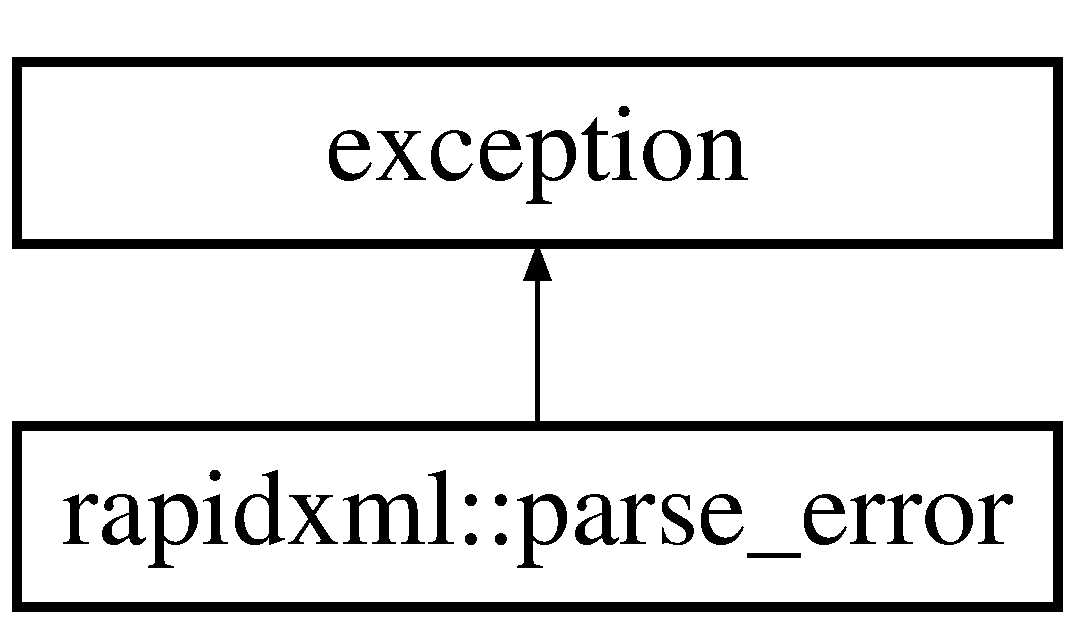
\includegraphics[height=2.000000cm]{classrapidxml_1_1parse__error}
\end{center}
\end{figure}
\subsection*{Public Member Functions}
\begin{DoxyCompactItemize}
\item 
\hypertarget{classrapidxml_1_1parse__error_aea12a301271c393fb627b368fb9f35c1}{\hyperlink{classrapidxml_1_1parse__error_aea12a301271c393fb627b368fb9f35c1}{parse\-\_\-error} (const char $\ast$\hyperlink{classrapidxml_1_1parse__error_a7665c88639e7466ee1de388a4f85e6fe}{what}, void $\ast$\hyperlink{classrapidxml_1_1parse__error_a3a0ab9e586c1d2b437c340f6622fbec6}{where})}\label{classrapidxml_1_1parse__error_aea12a301271c393fb627b368fb9f35c1}

\begin{DoxyCompactList}\small\item\em Constructs parse error. \end{DoxyCompactList}\item 
virtual const char $\ast$ \hyperlink{classrapidxml_1_1parse__error_a7665c88639e7466ee1de388a4f85e6fe}{what} () const   throw ()
\item 
{\footnotesize template$<$class Ch $>$ }\\Ch $\ast$ \hyperlink{classrapidxml_1_1parse__error_a3a0ab9e586c1d2b437c340f6622fbec6}{where} () const 
\end{DoxyCompactItemize}


\subsection{Detailed Description}
Parse error exception. This exception is thrown by the parser when an error occurs. Use \hyperlink{classrapidxml_1_1parse__error_a7665c88639e7466ee1de388a4f85e6fe}{what()} function to get human-\/readable error message. Use \hyperlink{classrapidxml_1_1parse__error_a3a0ab9e586c1d2b437c340f6622fbec6}{where()} function to get a pointer to position within source text where error was detected. \par
\par
 If throwing exceptions by the parser is undesirable, it can be disabled by defining R\-A\-P\-I\-D\-X\-M\-L\-\_\-\-N\-O\-\_\-\-E\-X\-C\-E\-P\-T\-I\-O\-N\-S macro before \hyperlink{rapidxml_8hpp}{rapidxml.\-hpp} is included. This will cause the parser to call rapidxml\-::parse\-\_\-error\-\_\-handler() function instead of throwing an exception. This function must be defined by the user. \par
\par
 This class derives from {\ttfamily std\-::exception} class. 

\subsection{Member Function Documentation}
\hypertarget{classrapidxml_1_1parse__error_a7665c88639e7466ee1de388a4f85e6fe}{\index{rapidxml\-::parse\-\_\-error@{rapidxml\-::parse\-\_\-error}!what@{what}}
\index{what@{what}!rapidxml::parse_error@{rapidxml\-::parse\-\_\-error}}
\subsubsection[{what}]{\setlength{\rightskip}{0pt plus 5cm}virtual const char$\ast$ rapidxml\-::parse\-\_\-error\-::what (
\begin{DoxyParamCaption}
{}
\end{DoxyParamCaption}
) const throw  ) \hspace{0.3cm}{\ttfamily [inline]}, {\ttfamily [virtual]}}}\label{classrapidxml_1_1parse__error_a7665c88639e7466ee1de388a4f85e6fe}
Gets human readable description of error. \begin{DoxyReturn}{Returns}
Pointer to null terminated description of the error. 
\end{DoxyReturn}
\hypertarget{classrapidxml_1_1parse__error_a3a0ab9e586c1d2b437c340f6622fbec6}{\index{rapidxml\-::parse\-\_\-error@{rapidxml\-::parse\-\_\-error}!where@{where}}
\index{where@{where}!rapidxml::parse_error@{rapidxml\-::parse\-\_\-error}}
\subsubsection[{where}]{\setlength{\rightskip}{0pt plus 5cm}template$<$class Ch $>$ Ch$\ast$ rapidxml\-::parse\-\_\-error\-::where (
\begin{DoxyParamCaption}
{}
\end{DoxyParamCaption}
) const\hspace{0.3cm}{\ttfamily [inline]}}}\label{classrapidxml_1_1parse__error_a3a0ab9e586c1d2b437c340f6622fbec6}
Gets pointer to character data where error happened. Ch should be the same as char type of \hyperlink{classrapidxml_1_1xml__document}{xml\-\_\-document} that produced the error. \begin{DoxyReturn}{Returns}
Pointer to location within the parsed string where error occured. 
\end{DoxyReturn}


The documentation for this class was generated from the following file\-:\begin{DoxyCompactItemize}
\item 
rapidxml/\hyperlink{rapidxml_8hpp}{rapidxml.\-hpp}\end{DoxyCompactItemize}

\hypertarget{class_query_processor}{\section{Query\-Processor Class Reference}
\label{class_query_processor}\index{Query\-Processor@{Query\-Processor}}
}


\hyperlink{class_query_processor}{Query\-Processor} processes search queries entered by the user.  




{\ttfamily \#include $<$queryprocessor.\-h$>$}

\subsection*{Public Member Functions}
\begin{DoxyCompactItemize}
\item 
\hypertarget{class_query_processor_a32a6760ff0aab51b38fb8eb236e2e140}{\hyperlink{class_query_processor_a32a6760ff0aab51b38fb8eb236e2e140}{Query\-Processor} ()}\label{class_query_processor_a32a6760ff0aab51b38fb8eb236e2e140}

\begin{DoxyCompactList}\small\item\em \hyperlink{class_query_processor}{Query\-Processor} default constructor. \end{DoxyCompactList}\item 
\hyperlink{class_query_processor_aa9ad73b1a64d758e127d9d52f43201ce}{Query\-Processor} (\hyperlink{class_index_handler}{Index\-Handler} $\ast$\&ih, std\-::string \&search\-Text)
\begin{DoxyCompactList}\small\item\em \hyperlink{class_query_processor}{Query\-Processor} overloaded constructor. \end{DoxyCompactList}\end{DoxyCompactItemize}


\subsection{Detailed Description}
\hyperlink{class_query_processor}{Query\-Processor} processes search queries entered by the user. 

\subsection{Constructor \& Destructor Documentation}
\hypertarget{class_query_processor_aa9ad73b1a64d758e127d9d52f43201ce}{\index{Query\-Processor@{Query\-Processor}!Query\-Processor@{Query\-Processor}}
\index{Query\-Processor@{Query\-Processor}!QueryProcessor@{Query\-Processor}}
\subsubsection[{Query\-Processor}]{\setlength{\rightskip}{0pt plus 5cm}Query\-Processor\-::\-Query\-Processor (
\begin{DoxyParamCaption}
\item[{{\bf Index\-Handler} $\ast$\&}]{ih, }
\item[{std\-::string \&}]{search\-Text}
\end{DoxyParamCaption}
)}}\label{class_query_processor_aa9ad73b1a64d758e127d9d52f43201ce}


\hyperlink{class_query_processor}{Query\-Processor} overloaded constructor. 


\begin{DoxyParams}{Parameters}
{\em ih} & an \hyperlink{class_index_handler}{Index\-Handler} object. \\
\hline
{\em search\-Text} & a string containing the user's query. \\
\hline
\end{DoxyParams}


The documentation for this class was generated from the following files\-:\begin{DoxyCompactItemize}
\item 
queryprocessor.\-h\item 
queryprocessor.\-cpp\end{DoxyCompactItemize}

\hypertarget{classstemming_1_1stem}{\section{stemming\-:\-:stem$<$ string\-\_\-type\-T $>$ Class Template Reference}
\label{classstemming_1_1stem}\index{stemming\-::stem$<$ string\-\_\-type\-T $>$@{stemming\-::stem$<$ string\-\_\-type\-T $>$}}
}


\hyperlink{class_the}{The} base class for language-\/specific stemmers. \hyperlink{class_the}{The} template argument for the stemmers are the type of std\-::basic\-\_\-string that you are trying to stem, by default std\-::wstring (Unicode strings). As long as the char type of your basic\-\_\-string is wchar\-\_\-t, then you can use any type of basic\-\_\-string. This is to say, if your basic\-\_\-string has a custom char\-\_\-traits or allocator, then just specify it in your template argument to the stemmer. Example\-:  




{\ttfamily \#include $<$stemming.\-h$>$}

Inheritance diagram for stemming\-:\-:stem$<$ string\-\_\-type\-T $>$\-:\begin{figure}[H]
\begin{center}
\leavevmode
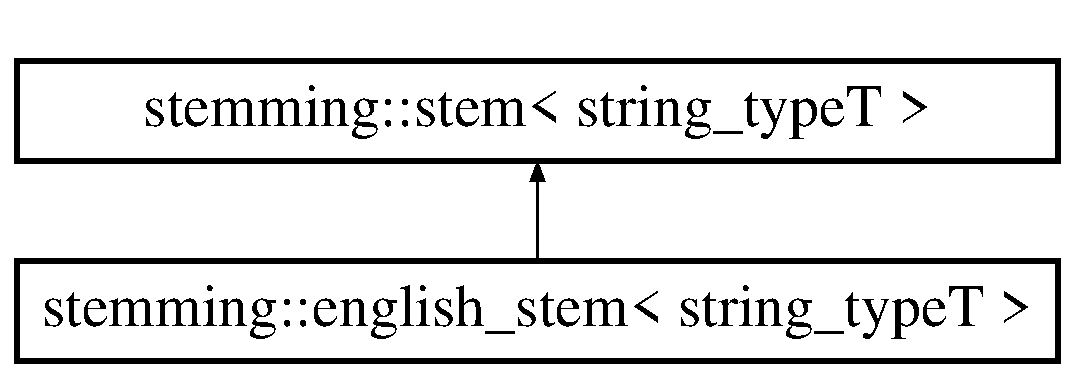
\includegraphics[height=2.000000cm]{classstemming_1_1stem}
\end{center}
\end{figure}
\subsection*{Protected Member Functions}
\begin{DoxyCompactItemize}
\item 
\hypertarget{group___stemming_ga364b7a76f683d5244715638069a4fa93}{void {\bfseries find\-\_\-r1} (const string\-\_\-type\-T \&text, const wchar\-\_\-t $\ast$vowel\-\_\-list)}\label{group___stemming_ga364b7a76f683d5244715638069a4fa93}

\item 
\hypertarget{group___stemming_gab381c0d6a6291c2c21515e9398e83085}{void {\bfseries find\-\_\-r2} (const string\-\_\-type\-T \&text, const wchar\-\_\-t $\ast$vowel\-\_\-list)}\label{group___stemming_gab381c0d6a6291c2c21515e9398e83085}

\item 
\hypertarget{group___stemming_gae6cb258098ba91462d421977b1eed8e7}{void {\bfseries find\-\_\-spanish\-\_\-rv} (const string\-\_\-type\-T \&text, const wchar\-\_\-t $\ast$vowel\-\_\-list)}\label{group___stemming_gae6cb258098ba91462d421977b1eed8e7}

\item 
\hypertarget{group___stemming_ga9626e49b982eda0d8ec3bb861d864b42}{void {\bfseries find\-\_\-french\-\_\-rv} (const string\-\_\-type\-T \&text, const wchar\-\_\-t $\ast$vowel\-\_\-list)}\label{group___stemming_ga9626e49b982eda0d8ec3bb861d864b42}

\item 
\hypertarget{group___stemming_ga53dcfe6b18fe5b5882474f222190ef1b}{void {\bfseries find\-\_\-russian\-\_\-rv} (const string\-\_\-type\-T \&text, const wchar\-\_\-t $\ast$vowel\-\_\-list)}\label{group___stemming_ga53dcfe6b18fe5b5882474f222190ef1b}

\item 
\hypertarget{group___stemming_ga9dcc3d89844ecd5c81eabf80936a0209}{void {\bfseries update\-\_\-r\-\_\-sections} (const string\-\_\-type\-T \&text)}\label{group___stemming_ga9dcc3d89844ecd5c81eabf80936a0209}

\item 
bool \hyperlink{group___stemming_ga0b423c8a1a53ec586da4613472d61e34}{is\-\_\-apostrophe} (const wchar\-\_\-t \&ch) const 
\item 
\hypertarget{group___stemming_ga36818a956dd34c388fa9942ed46e28b4}{void {\bfseries trim\-\_\-western\-\_\-punctuation} (string\-\_\-type\-T \&text) const }\label{group___stemming_ga36818a956dd34c388fa9942ed46e28b4}

\item 
\hypertarget{group___stemming_gac318ddd46a716673edf3678c47d3035c}{bool \hyperlink{group___stemming_gac318ddd46a716673edf3678c47d3035c}{is\-\_\-suffix} (const string\-\_\-type\-T \&text, const wchar\-\_\-t suffix1\-L, const wchar\-\_\-t suffix1\-U) const }\label{group___stemming_gac318ddd46a716673edf3678c47d3035c}

\begin{DoxyCompactList}\small\item\em is\-\_\-suffix for one character \end{DoxyCompactList}\item 
\hypertarget{group___stemming_gaad4dff424a3ae8a82dcfe6adac7c9d30}{bool \hyperlink{group___stemming_gaad4dff424a3ae8a82dcfe6adac7c9d30}{is\-\_\-suffix} (const string\-\_\-type\-T \&text, const wchar\-\_\-t suffix1\-L, const wchar\-\_\-t suffix1\-U, const wchar\-\_\-t suffix2\-L, const wchar\-\_\-t suffix2\-U) const }\label{group___stemming_gaad4dff424a3ae8a82dcfe6adac7c9d30}

\begin{DoxyCompactList}\small\item\em is\-\_\-suffix for two characters \end{DoxyCompactList}\item 
\hypertarget{group___stemming_gabbe6496d43b49dab0745e6d6b4e2831d}{bool \hyperlink{group___stemming_gabbe6496d43b49dab0745e6d6b4e2831d}{is\-\_\-suffix} (const string\-\_\-type\-T \&text, const wchar\-\_\-t suffix1\-L, const wchar\-\_\-t suffix1\-U, const wchar\-\_\-t suffix2\-L, const wchar\-\_\-t suffix2\-U, const wchar\-\_\-t suffix3\-L, const wchar\-\_\-t suffix3\-U) const }\label{group___stemming_gabbe6496d43b49dab0745e6d6b4e2831d}

\begin{DoxyCompactList}\small\item\em is\-\_\-suffix for three characters \end{DoxyCompactList}\item 
\hypertarget{group___stemming_ga694dd20e52adc89edadf120bf92a28ff}{bool \hyperlink{group___stemming_ga694dd20e52adc89edadf120bf92a28ff}{is\-\_\-suffix} (const string\-\_\-type\-T \&text, const wchar\-\_\-t suffix1\-L, const wchar\-\_\-t suffix1\-U, const wchar\-\_\-t suffix2\-L, const wchar\-\_\-t suffix2\-U, const wchar\-\_\-t suffix3\-L, const wchar\-\_\-t suffix3\-U, const wchar\-\_\-t suffix4\-L, const wchar\-\_\-t suffix4\-U) const }\label{group___stemming_ga694dd20e52adc89edadf120bf92a28ff}

\begin{DoxyCompactList}\small\item\em is\-\_\-suffix for four characters \end{DoxyCompactList}\item 
\hypertarget{group___stemming_ga001757aa7530b8acea05df8405def025}{bool \hyperlink{group___stemming_ga001757aa7530b8acea05df8405def025}{is\-\_\-suffix} (const string\-\_\-type\-T \&text, const wchar\-\_\-t suffix1\-L, const wchar\-\_\-t suffix1\-U, const wchar\-\_\-t suffix2\-L, const wchar\-\_\-t suffix2\-U, const wchar\-\_\-t suffix3\-L, const wchar\-\_\-t suffix3\-U, const wchar\-\_\-t suffix4\-L, const wchar\-\_\-t suffix4\-U, const wchar\-\_\-t suffix5\-L, const wchar\-\_\-t suffix5\-U) const }\label{group___stemming_ga001757aa7530b8acea05df8405def025}

\begin{DoxyCompactList}\small\item\em is\-\_\-suffix for five characters \end{DoxyCompactList}\item 
\hypertarget{group___stemming_gabe83f7592028b43f5cec9ce35ae1d9df}{bool \hyperlink{group___stemming_gabe83f7592028b43f5cec9ce35ae1d9df}{is\-\_\-suffix} (const string\-\_\-type\-T \&text, const wchar\-\_\-t suffix1\-L, const wchar\-\_\-t suffix1\-U, const wchar\-\_\-t suffix2\-L, const wchar\-\_\-t suffix2\-U, const wchar\-\_\-t suffix3\-L, const wchar\-\_\-t suffix3\-U, const wchar\-\_\-t suffix4\-L, const wchar\-\_\-t suffix4\-U, const wchar\-\_\-t suffix5\-L, const wchar\-\_\-t suffix5\-U, const wchar\-\_\-t suffix6\-L, const wchar\-\_\-t suffix6\-U) const }\label{group___stemming_gabe83f7592028b43f5cec9ce35ae1d9df}

\begin{DoxyCompactList}\small\item\em is\-\_\-suffix for six characters \end{DoxyCompactList}\item 
\hypertarget{group___stemming_ga79f18e256337d37054c80de470660a65}{bool \hyperlink{group___stemming_ga79f18e256337d37054c80de470660a65}{is\-\_\-suffix} (const string\-\_\-type\-T \&text, const wchar\-\_\-t suffix1\-L, const wchar\-\_\-t suffix1\-U, const wchar\-\_\-t suffix2\-L, const wchar\-\_\-t suffix2\-U, const wchar\-\_\-t suffix3\-L, const wchar\-\_\-t suffix3\-U, const wchar\-\_\-t suffix4\-L, const wchar\-\_\-t suffix4\-U, const wchar\-\_\-t suffix5\-L, const wchar\-\_\-t suffix5\-U, const wchar\-\_\-t suffix6\-L, const wchar\-\_\-t suffix6\-U, const wchar\-\_\-t suffix7\-L, const wchar\-\_\-t suffix7\-U) const }\label{group___stemming_ga79f18e256337d37054c80de470660a65}

\begin{DoxyCompactList}\small\item\em is\-\_\-suffix for seven characters \end{DoxyCompactList}\item 
\hypertarget{group___stemming_gaa18daf5b33d220d93dff22d6e591edd6}{bool \hyperlink{group___stemming_gaa18daf5b33d220d93dff22d6e591edd6}{is\-\_\-suffix} (const string\-\_\-type\-T \&text, const wchar\-\_\-t suffix1\-L, const wchar\-\_\-t suffix1\-U, const wchar\-\_\-t suffix2\-L, const wchar\-\_\-t suffix2\-U, const wchar\-\_\-t suffix3\-L, const wchar\-\_\-t suffix3\-U, const wchar\-\_\-t suffix4\-L, const wchar\-\_\-t suffix4\-U, const wchar\-\_\-t suffix5\-L, const wchar\-\_\-t suffix5\-U, const wchar\-\_\-t suffix6\-L, const wchar\-\_\-t suffix6\-U, const wchar\-\_\-t suffix7\-L, const wchar\-\_\-t suffix7\-U, const wchar\-\_\-t suffix8\-L, const wchar\-\_\-t suffix8\-U) const }\label{group___stemming_gaa18daf5b33d220d93dff22d6e591edd6}

\begin{DoxyCompactList}\small\item\em is\-\_\-suffix for eight characters \end{DoxyCompactList}\item 
\hypertarget{group___stemming_gab905150e381f068c6b04eba851bb6263}{bool \hyperlink{group___stemming_gab905150e381f068c6b04eba851bb6263}{is\-\_\-suffix} (const string\-\_\-type\-T \&text, const wchar\-\_\-t suffix1\-L, const wchar\-\_\-t suffix1\-U, const wchar\-\_\-t suffix2\-L, const wchar\-\_\-t suffix2\-U, const wchar\-\_\-t suffix3\-L, const wchar\-\_\-t suffix3\-U, const wchar\-\_\-t suffix4\-L, const wchar\-\_\-t suffix4\-U, const wchar\-\_\-t suffix5\-L, const wchar\-\_\-t suffix5\-U, const wchar\-\_\-t suffix6\-L, const wchar\-\_\-t suffix6\-U, const wchar\-\_\-t suffix7\-L, const wchar\-\_\-t suffix7\-U, const wchar\-\_\-t suffix8\-L, const wchar\-\_\-t suffix8\-U, const wchar\-\_\-t suffix9\-L, const wchar\-\_\-t suffix9\-U) const }\label{group___stemming_gab905150e381f068c6b04eba851bb6263}

\begin{DoxyCompactList}\small\item\em is\-\_\-suffix for nine characters \end{DoxyCompactList}\item 
\hypertarget{group___stemming_ga2ae63cf92bc4f4f40f0093e4842a235f}{bool \hyperlink{group___stemming_ga2ae63cf92bc4f4f40f0093e4842a235f}{is\-\_\-partial\-\_\-suffix} (const string\-\_\-type\-T \&text, const size\-\_\-t start\-\_\-index, const wchar\-\_\-t suffix1\-L, const wchar\-\_\-t suffix1\-U, const wchar\-\_\-t suffix2\-L, const wchar\-\_\-t suffix2\-U)}\label{group___stemming_ga2ae63cf92bc4f4f40f0093e4842a235f}

\begin{DoxyCompactList}\small\item\em comparison for two characters \end{DoxyCompactList}\item 
\hypertarget{group___stemming_ga728ea4e26737b04d04e02bea863f29e4}{bool \hyperlink{group___stemming_ga728ea4e26737b04d04e02bea863f29e4}{is\-\_\-partial\-\_\-suffix} (const string\-\_\-type\-T \&text, const size\-\_\-t start\-\_\-index, const wchar\-\_\-t suffix1\-L, const wchar\-\_\-t suffix1\-U, const wchar\-\_\-t suffix2\-L, const wchar\-\_\-t suffix2\-U, const wchar\-\_\-t suffix3\-L, const wchar\-\_\-t suffix3\-U)}\label{group___stemming_ga728ea4e26737b04d04e02bea863f29e4}

\begin{DoxyCompactList}\small\item\em comparison for three characters \end{DoxyCompactList}\item 
bool \hyperlink{group___stemming_ga2c92d7447b5cc97d0fca165d2b0e7d68}{is\-\_\-suffix\-\_\-in\-\_\-rv} (const string\-\_\-type\-T \&text, const wchar\-\_\-t suffix1\-L, const wchar\-\_\-t suffix1\-U)
\begin{DoxyCompactList}\small\item\em R\-V suffix functions. \end{DoxyCompactList}\item 
\hypertarget{group___stemming_ga359356fbaafc3c7154d94fda6916ffa0}{bool \hyperlink{group___stemming_ga359356fbaafc3c7154d94fda6916ffa0}{is\-\_\-suffix\-\_\-in\-\_\-rv} (const string\-\_\-type\-T \&text, const wchar\-\_\-t suffix1\-L, const wchar\-\_\-t suffix1\-U, const wchar\-\_\-t suffix2\-L, const wchar\-\_\-t suffix2\-U)}\label{group___stemming_ga359356fbaafc3c7154d94fda6916ffa0}

\begin{DoxyCompactList}\small\item\em R\-V suffix comparison for two characters. \end{DoxyCompactList}\item 
\hypertarget{group___stemming_ga00fa5d00ff53320a437fe96a5bfa8f44}{bool \hyperlink{group___stemming_ga00fa5d00ff53320a437fe96a5bfa8f44}{is\-\_\-suffix\-\_\-in\-\_\-rv} (const string\-\_\-type\-T \&text, const wchar\-\_\-t suffix1\-L, const wchar\-\_\-t suffix1\-U, const wchar\-\_\-t suffix2\-L, const wchar\-\_\-t suffix2\-U, const wchar\-\_\-t suffix3\-L, const wchar\-\_\-t suffix3\-U)}\label{group___stemming_ga00fa5d00ff53320a437fe96a5bfa8f44}

\begin{DoxyCompactList}\small\item\em R\-V suffix comparison for three characters. \end{DoxyCompactList}\item 
\hypertarget{group___stemming_gacdaff4e73f7f3841beed04775b5d4f21}{bool \hyperlink{group___stemming_gacdaff4e73f7f3841beed04775b5d4f21}{is\-\_\-suffix\-\_\-in\-\_\-rv} (const string\-\_\-type\-T \&text, const wchar\-\_\-t suffix1\-L, const wchar\-\_\-t suffix1\-U, const wchar\-\_\-t suffix2\-L, const wchar\-\_\-t suffix2\-U, const wchar\-\_\-t suffix3\-L, const wchar\-\_\-t suffix3\-U, const wchar\-\_\-t suffix4\-L, const wchar\-\_\-t suffix4\-U)}\label{group___stemming_gacdaff4e73f7f3841beed04775b5d4f21}

\begin{DoxyCompactList}\small\item\em R\-V suffix comparison for four characters. \end{DoxyCompactList}\item 
\hypertarget{group___stemming_ga99ef9b0e80da18c39cc0206a666bd4b1}{bool \hyperlink{group___stemming_ga99ef9b0e80da18c39cc0206a666bd4b1}{is\-\_\-suffix\-\_\-in\-\_\-rv} (const string\-\_\-type\-T \&text, const wchar\-\_\-t suffix1\-L, const wchar\-\_\-t suffix1\-U, const wchar\-\_\-t suffix2\-L, const wchar\-\_\-t suffix2\-U, const wchar\-\_\-t suffix3\-L, const wchar\-\_\-t suffix3\-U, const wchar\-\_\-t suffix4\-L, const wchar\-\_\-t suffix4\-U, const wchar\-\_\-t suffix5\-L, const wchar\-\_\-t suffix5\-U)}\label{group___stemming_ga99ef9b0e80da18c39cc0206a666bd4b1}

\begin{DoxyCompactList}\small\item\em R\-V suffix comparison for five characters. \end{DoxyCompactList}\item 
\hypertarget{group___stemming_ga527b081fee02f191713a50dbc396f986}{bool \hyperlink{group___stemming_ga527b081fee02f191713a50dbc396f986}{is\-\_\-suffix\-\_\-in\-\_\-rv} (const string\-\_\-type\-T \&text, const wchar\-\_\-t suffix1\-L, const wchar\-\_\-t suffix1\-U, const wchar\-\_\-t suffix2\-L, const wchar\-\_\-t suffix2\-U, const wchar\-\_\-t suffix3\-L, const wchar\-\_\-t suffix3\-U, const wchar\-\_\-t suffix4\-L, const wchar\-\_\-t suffix4\-U, const wchar\-\_\-t suffix5\-L, const wchar\-\_\-t suffix5\-U, const wchar\-\_\-t suffix6\-L, const wchar\-\_\-t suffix6\-U)}\label{group___stemming_ga527b081fee02f191713a50dbc396f986}

\begin{DoxyCompactList}\small\item\em R\-V suffix comparison for six characters. \end{DoxyCompactList}\item 
\hypertarget{group___stemming_gabd6431b54fc5175c29809c627c44a587}{bool \hyperlink{group___stemming_gabd6431b54fc5175c29809c627c44a587}{is\-\_\-suffix\-\_\-in\-\_\-rv} (const string\-\_\-type\-T \&text, const wchar\-\_\-t suffix1\-L, const wchar\-\_\-t suffix1\-U, const wchar\-\_\-t suffix2\-L, const wchar\-\_\-t suffix2\-U, const wchar\-\_\-t suffix3\-L, const wchar\-\_\-t suffix3\-U, const wchar\-\_\-t suffix4\-L, const wchar\-\_\-t suffix4\-U, const wchar\-\_\-t suffix5\-L, const wchar\-\_\-t suffix5\-U, const wchar\-\_\-t suffix6\-L, const wchar\-\_\-t suffix6\-U, const wchar\-\_\-t suffix7\-L, const wchar\-\_\-t suffix7\-U)}\label{group___stemming_gabd6431b54fc5175c29809c627c44a587}

\begin{DoxyCompactList}\small\item\em R\-V suffix comparison for seven characters. \end{DoxyCompactList}\item 
\hypertarget{group___stemming_ga553b6ed34e6b03e2c1ca42ea2db08ba6}{bool \hyperlink{group___stemming_ga553b6ed34e6b03e2c1ca42ea2db08ba6}{is\-\_\-suffix\-\_\-in\-\_\-rv} (const string\-\_\-type\-T \&text, const wchar\-\_\-t suffix1\-L, const wchar\-\_\-t suffix1\-U, const wchar\-\_\-t suffix2\-L, const wchar\-\_\-t suffix2\-U, const wchar\-\_\-t suffix3\-L, const wchar\-\_\-t suffix3\-U, const wchar\-\_\-t suffix4\-L, const wchar\-\_\-t suffix4\-U, const wchar\-\_\-t suffix5\-L, const wchar\-\_\-t suffix5\-U, const wchar\-\_\-t suffix6\-L, const wchar\-\_\-t suffix6\-U, const wchar\-\_\-t suffix7\-L, const wchar\-\_\-t suffix7\-U, const wchar\-\_\-t suffix8\-L, const wchar\-\_\-t suffix8\-U)}\label{group___stemming_ga553b6ed34e6b03e2c1ca42ea2db08ba6}

\begin{DoxyCompactList}\small\item\em R\-V suffix comparison for eight characters. \end{DoxyCompactList}\item 
bool \hyperlink{group___stemming_gaefe544e653b27bd5c1fab7b5a18d80a1}{is\-\_\-suffix\-\_\-in\-\_\-r1} (const string\-\_\-type\-T \&text, const wchar\-\_\-t suffix1\-L, const wchar\-\_\-t suffix1\-U)
\begin{DoxyCompactList}\small\item\em R1 suffix functions. \end{DoxyCompactList}\item 
\hypertarget{group___stemming_gab8cb2e00b39091f74b1064e1f0314c6f}{bool \hyperlink{group___stemming_gab8cb2e00b39091f74b1064e1f0314c6f}{is\-\_\-suffix\-\_\-in\-\_\-r1} (const string\-\_\-type\-T \&text, const wchar\-\_\-t suffix1\-L, const wchar\-\_\-t suffix1\-U, const wchar\-\_\-t suffix2\-L, const wchar\-\_\-t suffix2\-U)}\label{group___stemming_gab8cb2e00b39091f74b1064e1f0314c6f}

\begin{DoxyCompactList}\small\item\em R1 suffix comparison for two characters. \end{DoxyCompactList}\item 
\hypertarget{group___stemming_ga1fe4a63adfa5d4f378a060352d52edc1}{bool \hyperlink{group___stemming_ga1fe4a63adfa5d4f378a060352d52edc1}{is\-\_\-suffix\-\_\-in\-\_\-r1} (const string\-\_\-type\-T \&text, const wchar\-\_\-t suffix1\-L, const wchar\-\_\-t suffix1\-U, const wchar\-\_\-t suffix2\-L, const wchar\-\_\-t suffix2\-U, const wchar\-\_\-t suffix3\-L, const wchar\-\_\-t suffix3\-U)}\label{group___stemming_ga1fe4a63adfa5d4f378a060352d52edc1}

\begin{DoxyCompactList}\small\item\em R1 suffix comparison for three characters. \end{DoxyCompactList}\item 
\hypertarget{group___stemming_ga3fef2f8916933fa1965928f8e43a1b58}{bool \hyperlink{group___stemming_ga3fef2f8916933fa1965928f8e43a1b58}{is\-\_\-suffix\-\_\-in\-\_\-r1} (const string\-\_\-type\-T \&text, const wchar\-\_\-t suffix1\-L, const wchar\-\_\-t suffix1\-U, const wchar\-\_\-t suffix2\-L, const wchar\-\_\-t suffix2\-U, const wchar\-\_\-t suffix3\-L, const wchar\-\_\-t suffix3\-U, const wchar\-\_\-t suffix4\-L, const wchar\-\_\-t suffix4\-U)}\label{group___stemming_ga3fef2f8916933fa1965928f8e43a1b58}

\begin{DoxyCompactList}\small\item\em R1 suffix comparison for four characters. \end{DoxyCompactList}\item 
\hypertarget{group___stemming_ga88f0e5e0cc055f013b6321215eb18ef3}{bool \hyperlink{group___stemming_ga88f0e5e0cc055f013b6321215eb18ef3}{is\-\_\-suffix\-\_\-in\-\_\-r1} (const string\-\_\-type\-T \&text, const wchar\-\_\-t suffix1\-L, const wchar\-\_\-t suffix1\-U, const wchar\-\_\-t suffix2\-L, const wchar\-\_\-t suffix2\-U, const wchar\-\_\-t suffix3\-L, const wchar\-\_\-t suffix3\-U, const wchar\-\_\-t suffix4\-L, const wchar\-\_\-t suffix4\-U, const wchar\-\_\-t suffix5\-L, const wchar\-\_\-t suffix5\-U)}\label{group___stemming_ga88f0e5e0cc055f013b6321215eb18ef3}

\begin{DoxyCompactList}\small\item\em R1 suffix comparison for five characters. \end{DoxyCompactList}\item 
\hypertarget{group___stemming_ga19c2ee5166c7a9c81160408438c1f9a0}{bool \hyperlink{group___stemming_ga19c2ee5166c7a9c81160408438c1f9a0}{is\-\_\-suffix\-\_\-in\-\_\-r1} (const string\-\_\-type\-T \&text, const wchar\-\_\-t suffix1\-L, const wchar\-\_\-t suffix1\-U, const wchar\-\_\-t suffix2\-L, const wchar\-\_\-t suffix2\-U, const wchar\-\_\-t suffix3\-L, const wchar\-\_\-t suffix3\-U, const wchar\-\_\-t suffix4\-L, const wchar\-\_\-t suffix4\-U, const wchar\-\_\-t suffix5\-L, const wchar\-\_\-t suffix5\-U, const wchar\-\_\-t suffix6\-L, const wchar\-\_\-t suffix6\-U)}\label{group___stemming_ga19c2ee5166c7a9c81160408438c1f9a0}

\begin{DoxyCompactList}\small\item\em R1 suffix comparison for six characters. \end{DoxyCompactList}\item 
bool \hyperlink{group___stemming_gac2c9cace7e6d90ca0b8c08f2ca2809e3}{is\-\_\-suffix\-\_\-in\-\_\-r2} (const string\-\_\-type\-T \&text, const wchar\-\_\-t suffix1\-L, const wchar\-\_\-t suffix1\-U)
\begin{DoxyCompactList}\small\item\em R2 suffix functions. \end{DoxyCompactList}\item 
\hypertarget{group___stemming_ga8325bde2b5c8d5676d2b8e2b822b29a4}{bool \hyperlink{group___stemming_ga8325bde2b5c8d5676d2b8e2b822b29a4}{is\-\_\-suffix\-\_\-in\-\_\-r2} (const string\-\_\-type\-T \&text, const wchar\-\_\-t suffix1\-L, const wchar\-\_\-t suffix1\-U, const wchar\-\_\-t suffix2\-L, const wchar\-\_\-t suffix2\-U)}\label{group___stemming_ga8325bde2b5c8d5676d2b8e2b822b29a4}

\begin{DoxyCompactList}\small\item\em R2 suffix comparison for two characters. \end{DoxyCompactList}\item 
\hypertarget{group___stemming_gab5c71d01e3285eec2e79521c1b76f79d}{bool \hyperlink{group___stemming_gab5c71d01e3285eec2e79521c1b76f79d}{is\-\_\-suffix\-\_\-in\-\_\-r2} (const string\-\_\-type\-T \&text, const wchar\-\_\-t suffix1\-L, const wchar\-\_\-t suffix1\-U, const wchar\-\_\-t suffix2\-L, const wchar\-\_\-t suffix2\-U, const wchar\-\_\-t suffix3\-L, const wchar\-\_\-t suffix3\-U)}\label{group___stemming_gab5c71d01e3285eec2e79521c1b76f79d}

\begin{DoxyCompactList}\small\item\em R2 suffix comparison for three characters. \end{DoxyCompactList}\item 
\hypertarget{group___stemming_gac12e9f11d41f69e71c7379387c4564b9}{bool \hyperlink{group___stemming_gac12e9f11d41f69e71c7379387c4564b9}{is\-\_\-suffix\-\_\-in\-\_\-r2} (const string\-\_\-type\-T \&text, const wchar\-\_\-t suffix1\-L, const wchar\-\_\-t suffix1\-U, const wchar\-\_\-t suffix2\-L, const wchar\-\_\-t suffix2\-U, const wchar\-\_\-t suffix3\-L, const wchar\-\_\-t suffix3\-U, const wchar\-\_\-t suffix4\-L, const wchar\-\_\-t suffix4\-U)}\label{group___stemming_gac12e9f11d41f69e71c7379387c4564b9}

\begin{DoxyCompactList}\small\item\em R2 suffix comparison for four characters. \end{DoxyCompactList}\item 
\hypertarget{group___stemming_gaca8fba0d6b27d8da969508adc281cfa5}{bool \hyperlink{group___stemming_gaca8fba0d6b27d8da969508adc281cfa5}{is\-\_\-suffix\-\_\-in\-\_\-r2} (const string\-\_\-type\-T \&text, const wchar\-\_\-t suffix1\-L, const wchar\-\_\-t suffix1\-U, const wchar\-\_\-t suffix2\-L, const wchar\-\_\-t suffix2\-U, const wchar\-\_\-t suffix3\-L, const wchar\-\_\-t suffix3\-U, const wchar\-\_\-t suffix4\-L, const wchar\-\_\-t suffix4\-U, const wchar\-\_\-t suffix5\-L, const wchar\-\_\-t suffix5\-U)}\label{group___stemming_gaca8fba0d6b27d8da969508adc281cfa5}

\begin{DoxyCompactList}\small\item\em R2 suffix comparison for five characters. \end{DoxyCompactList}\item 
\hypertarget{group___stemming_gad85a9757083c5fcbd6300367df2a648b}{bool \hyperlink{group___stemming_gad85a9757083c5fcbd6300367df2a648b}{is\-\_\-suffix\-\_\-in\-\_\-r2} (string\-\_\-type\-T \&text, const wchar\-\_\-t suffix1\-L, const wchar\-\_\-t suffix1\-U, const wchar\-\_\-t suffix2\-L, const wchar\-\_\-t suffix2\-U, const wchar\-\_\-t suffix3\-L, const wchar\-\_\-t suffix3\-U, const wchar\-\_\-t suffix4\-L, const wchar\-\_\-t suffix4\-U, const wchar\-\_\-t suffix5\-L, const wchar\-\_\-t suffix5\-U, const wchar\-\_\-t suffix6\-L, const wchar\-\_\-t suffix6\-U)}\label{group___stemming_gad85a9757083c5fcbd6300367df2a648b}

\begin{DoxyCompactList}\small\item\em R2 suffix comparison for six characters. \end{DoxyCompactList}\item 
\hypertarget{group___stemming_ga65e9882d17885e66208840b277fcee2e}{bool \hyperlink{group___stemming_ga65e9882d17885e66208840b277fcee2e}{is\-\_\-suffix\-\_\-in\-\_\-r2} (const string\-\_\-type\-T \&text, const wchar\-\_\-t suffix1\-L, const wchar\-\_\-t suffix1\-U, const wchar\-\_\-t suffix2\-L, const wchar\-\_\-t suffix2\-U, const wchar\-\_\-t suffix3\-L, const wchar\-\_\-t suffix3\-U, const wchar\-\_\-t suffix4\-L, const wchar\-\_\-t suffix4\-U, const wchar\-\_\-t suffix5\-L, const wchar\-\_\-t suffix5\-U, const wchar\-\_\-t suffix6\-L, const wchar\-\_\-t suffix6\-U, const wchar\-\_\-t suffix7\-L, const wchar\-\_\-t suffix7\-U)}\label{group___stemming_ga65e9882d17885e66208840b277fcee2e}

\begin{DoxyCompactList}\small\item\em R2 suffix comparison for seven characters. \end{DoxyCompactList}\item 
\hypertarget{group___stemming_ga3bda630783eae1661f00fc5d2b51ce5c}{bool {\bfseries delete\-\_\-if\-\_\-is\-\_\-in\-\_\-r1} (string\-\_\-type\-T \&text, const wchar\-\_\-t suffix1\-L, const wchar\-\_\-t suffix1\-U, const bool success\-\_\-on\-\_\-find=true)}\label{group___stemming_ga3bda630783eae1661f00fc5d2b51ce5c}

\item 
\hypertarget{group___stemming_ga843e54b874cbb56a5d5997987137c933}{bool {\bfseries delete\-\_\-if\-\_\-is\-\_\-in\-\_\-r1} (string\-\_\-type\-T \&text, const wchar\-\_\-t suffix1\-L, const wchar\-\_\-t suffix1\-U, const wchar\-\_\-t suffix2\-L, const wchar\-\_\-t suffix2\-U, const bool success\-\_\-on\-\_\-find=true)}\label{group___stemming_ga843e54b874cbb56a5d5997987137c933}

\item 
\hypertarget{group___stemming_gaf5c33c5c4644373cd85390c7e3282084}{bool {\bfseries delete\-\_\-if\-\_\-is\-\_\-in\-\_\-r1} (string\-\_\-type\-T \&text, const wchar\-\_\-t suffix1\-L, const wchar\-\_\-t suffix1\-U, const wchar\-\_\-t suffix2\-L, const wchar\-\_\-t suffix2\-U, const wchar\-\_\-t suffix3\-L, const wchar\-\_\-t suffix3\-U, const bool success\-\_\-on\-\_\-find=true)}\label{group___stemming_gaf5c33c5c4644373cd85390c7e3282084}

\item 
\hypertarget{group___stemming_ga6be1595a7c29fec666ff808701be3eb2}{bool {\bfseries delete\-\_\-if\-\_\-is\-\_\-in\-\_\-r1} (string\-\_\-type\-T \&text, const wchar\-\_\-t suffix1\-L, const wchar\-\_\-t suffix1\-U, const wchar\-\_\-t suffix2\-L, const wchar\-\_\-t suffix2\-U, const wchar\-\_\-t suffix3\-L, const wchar\-\_\-t suffix3\-U, const wchar\-\_\-t suffix4\-L, const wchar\-\_\-t suffix4\-U, const bool success\-\_\-on\-\_\-find=true)}\label{group___stemming_ga6be1595a7c29fec666ff808701be3eb2}

\item 
\hypertarget{group___stemming_gabac9ef13a80efee3dad9b72476f7cd49}{bool {\bfseries delete\-\_\-if\-\_\-is\-\_\-in\-\_\-r1} (string\-\_\-type\-T \&text, const wchar\-\_\-t suffix1\-L, const wchar\-\_\-t suffix1\-U, const wchar\-\_\-t suffix2\-L, const wchar\-\_\-t suffix2\-U, const wchar\-\_\-t suffix3\-L, const wchar\-\_\-t suffix3\-U, const wchar\-\_\-t suffix4\-L, const wchar\-\_\-t suffix4\-U, const wchar\-\_\-t suffix5\-L, const wchar\-\_\-t suffix5\-U, const bool success\-\_\-on\-\_\-find=true)}\label{group___stemming_gabac9ef13a80efee3dad9b72476f7cd49}

\item 
\hypertarget{group___stemming_ga3fbbd1cbf322889ba4e4940d87449bb0}{bool {\bfseries delete\-\_\-if\-\_\-is\-\_\-in\-\_\-r1} (string\-\_\-type\-T \&text, const wchar\-\_\-t suffix1\-L, const wchar\-\_\-t suffix1\-U, const wchar\-\_\-t suffix2\-L, const wchar\-\_\-t suffix2\-U, const wchar\-\_\-t suffix3\-L, const wchar\-\_\-t suffix3\-U, const wchar\-\_\-t suffix4\-L, const wchar\-\_\-t suffix4\-U, const wchar\-\_\-t suffix5\-L, const wchar\-\_\-t suffix5\-U, const wchar\-\_\-t suffix6\-L, const wchar\-\_\-t suffix6\-U, const bool success\-\_\-on\-\_\-find=true)}\label{group___stemming_ga3fbbd1cbf322889ba4e4940d87449bb0}

\item 
\hypertarget{group___stemming_gacdf0457bd3392f1ac23dadef5515cebd}{bool {\bfseries delete\-\_\-if\-\_\-is\-\_\-in\-\_\-r1} (string\-\_\-type\-T \&text, const wchar\-\_\-t suffix1\-L, const wchar\-\_\-t suffix1\-U, const wchar\-\_\-t suffix2\-L, const wchar\-\_\-t suffix2\-U, const wchar\-\_\-t suffix3\-L, const wchar\-\_\-t suffix3\-U, const wchar\-\_\-t suffix4\-L, const wchar\-\_\-t suffix4\-U, const wchar\-\_\-t suffix5\-L, const wchar\-\_\-t suffix5\-U, const wchar\-\_\-t suffix6\-L, const wchar\-\_\-t suffix6\-U, const wchar\-\_\-t suffix7\-L, const wchar\-\_\-t suffix7\-U, const bool success\-\_\-on\-\_\-find=true)}\label{group___stemming_gacdf0457bd3392f1ac23dadef5515cebd}

\item 
\hypertarget{group___stemming_ga722e75e6404934da2f0c9c00ffded48a}{bool {\bfseries delete\-\_\-if\-\_\-is\-\_\-in\-\_\-r2} (string\-\_\-type\-T \&text, const wchar\-\_\-t suffix1\-L, const wchar\-\_\-t suffix1\-U, const bool success\-\_\-on\-\_\-find=true)}\label{group___stemming_ga722e75e6404934da2f0c9c00ffded48a}

\item 
\hypertarget{group___stemming_ga33bf1854d1748ba97e30ad798f828b0e}{bool {\bfseries delete\-\_\-if\-\_\-is\-\_\-in\-\_\-r2} (string\-\_\-type\-T \&text, const wchar\-\_\-t suffix1\-L, const wchar\-\_\-t suffix1\-U, const wchar\-\_\-t suffix2\-L, const wchar\-\_\-t suffix2\-U, const bool success\-\_\-on\-\_\-find=true)}\label{group___stemming_ga33bf1854d1748ba97e30ad798f828b0e}

\item 
\hypertarget{group___stemming_gac78dd58f01ed17a41eedc33d5b2deedb}{bool {\bfseries delete\-\_\-if\-\_\-is\-\_\-in\-\_\-r2} (string\-\_\-type\-T \&text, const wchar\-\_\-t suffix1\-L, const wchar\-\_\-t suffix1\-U, const wchar\-\_\-t suffix2\-L, const wchar\-\_\-t suffix2\-U, const wchar\-\_\-t suffix3\-L, const wchar\-\_\-t suffix3\-U, const bool success\-\_\-on\-\_\-find=true)}\label{group___stemming_gac78dd58f01ed17a41eedc33d5b2deedb}

\item 
\hypertarget{group___stemming_ga3a79fd0ac96d009d0c93f1bec847c2ff}{bool {\bfseries delete\-\_\-if\-\_\-is\-\_\-in\-\_\-r2} (string\-\_\-type\-T \&text, const wchar\-\_\-t suffix1\-L, const wchar\-\_\-t suffix1\-U, const wchar\-\_\-t suffix2\-L, const wchar\-\_\-t suffix2\-U, const wchar\-\_\-t suffix3\-L, const wchar\-\_\-t suffix3\-U, const wchar\-\_\-t suffix4\-L, const wchar\-\_\-t suffix4\-U, const bool success\-\_\-on\-\_\-find=true)}\label{group___stemming_ga3a79fd0ac96d009d0c93f1bec847c2ff}

\item 
\hypertarget{group___stemming_ga222f7af1124d34e58b3c38fa4b2ee669}{bool \hyperlink{group___stemming_ga222f7af1124d34e58b3c38fa4b2ee669}{delete\-\_\-if\-\_\-is\-\_\-in\-\_\-r2} (string\-\_\-type\-T \&text, const wchar\-\_\-t suffix1\-L, const wchar\-\_\-t suffix1\-U, const wchar\-\_\-t suffix2\-L, const wchar\-\_\-t suffix2\-U, const wchar\-\_\-t suffix3\-L, const wchar\-\_\-t suffix3\-U, const wchar\-\_\-t suffix4\-L, const wchar\-\_\-t suffix4\-U, const wchar\-\_\-t suffix5\-L, const wchar\-\_\-t suffix5\-U, const bool success\-\_\-on\-\_\-find=true)}\label{group___stemming_ga222f7af1124d34e58b3c38fa4b2ee669}

\begin{DoxyCompactList}\small\item\em R2 deletion for five character suffix. \end{DoxyCompactList}\item 
\hypertarget{group___stemming_ga95aca52d1f624638130a9d1c66570edb}{bool \hyperlink{group___stemming_ga95aca52d1f624638130a9d1c66570edb}{delete\-\_\-if\-\_\-is\-\_\-in\-\_\-r2} (string\-\_\-type\-T \&text, const wchar\-\_\-t suffix1\-L, const wchar\-\_\-t suffix1\-U, const wchar\-\_\-t suffix2\-L, const wchar\-\_\-t suffix2\-U, const wchar\-\_\-t suffix3\-L, const wchar\-\_\-t suffix3\-U, const wchar\-\_\-t suffix4\-L, const wchar\-\_\-t suffix4\-U, const wchar\-\_\-t suffix5\-L, const wchar\-\_\-t suffix5\-U, const wchar\-\_\-t suffix6\-L, const wchar\-\_\-t suffix6\-U, const bool success\-\_\-on\-\_\-find=true)}\label{group___stemming_ga95aca52d1f624638130a9d1c66570edb}

\begin{DoxyCompactList}\small\item\em R2 deletion for six character suffix. \end{DoxyCompactList}\item 
\hypertarget{group___stemming_ga9542e67a264c728cfb636767dc75a07c}{bool \hyperlink{group___stemming_ga9542e67a264c728cfb636767dc75a07c}{delete\-\_\-if\-\_\-is\-\_\-in\-\_\-r2} (string\-\_\-type\-T \&text, const wchar\-\_\-t suffix1\-L, const wchar\-\_\-t suffix1\-U, const wchar\-\_\-t suffix2\-L, const wchar\-\_\-t suffix2\-U, const wchar\-\_\-t suffix3\-L, const wchar\-\_\-t suffix3\-U, const wchar\-\_\-t suffix4\-L, const wchar\-\_\-t suffix4\-U, const wchar\-\_\-t suffix5\-L, const wchar\-\_\-t suffix5\-U, const wchar\-\_\-t suffix6\-L, const wchar\-\_\-t suffix6\-U, const wchar\-\_\-t suffix7\-L, const wchar\-\_\-t suffix7\-U, const bool success\-\_\-on\-\_\-find=true)}\label{group___stemming_ga9542e67a264c728cfb636767dc75a07c}

\begin{DoxyCompactList}\small\item\em R2 deletion for seven character suffix. \end{DoxyCompactList}\item 
\hypertarget{group___stemming_ga9bbc2192839ce8ebcf88d0220cfa2441}{bool \hyperlink{group___stemming_ga9bbc2192839ce8ebcf88d0220cfa2441}{delete\-\_\-if\-\_\-is\-\_\-in\-\_\-r2} (string\-\_\-type\-T \&text, const wchar\-\_\-t suffix1\-L, const wchar\-\_\-t suffix1\-U, const wchar\-\_\-t suffix2\-L, const wchar\-\_\-t suffix2\-U, const wchar\-\_\-t suffix3\-L, const wchar\-\_\-t suffix3\-U, const wchar\-\_\-t suffix4\-L, const wchar\-\_\-t suffix4\-U, const wchar\-\_\-t suffix5\-L, const wchar\-\_\-t suffix5\-U, const wchar\-\_\-t suffix6\-L, const wchar\-\_\-t suffix6\-U, const wchar\-\_\-t suffix7\-L, const wchar\-\_\-t suffix7\-U, const wchar\-\_\-t suffix8\-L, const wchar\-\_\-t suffix8\-U, const bool success\-\_\-on\-\_\-find=true)}\label{group___stemming_ga9bbc2192839ce8ebcf88d0220cfa2441}

\begin{DoxyCompactList}\small\item\em R2 deletion for eight character suffix. \end{DoxyCompactList}\item 
\hypertarget{group___stemming_ga3754d998db70ac20861ab3e87c3e5f25}{bool {\bfseries delete\-\_\-if\-\_\-is\-\_\-in\-\_\-rv} (string\-\_\-type\-T \&text, const wchar\-\_\-t suffix1\-L, const wchar\-\_\-t suffix1\-U, const bool success\-\_\-on\-\_\-find=true)}\label{group___stemming_ga3754d998db70ac20861ab3e87c3e5f25}

\item 
\hypertarget{group___stemming_ga5d0a95806d9264f7238bf425311d1dfc}{bool {\bfseries delete\-\_\-if\-\_\-is\-\_\-in\-\_\-rv} (string\-\_\-type\-T \&text, const wchar\-\_\-t suffix1\-L, const wchar\-\_\-t suffix1\-U, const wchar\-\_\-t suffix2\-L, const wchar\-\_\-t suffix2\-U, const bool success\-\_\-on\-\_\-find=true)}\label{group___stemming_ga5d0a95806d9264f7238bf425311d1dfc}

\item 
\hypertarget{group___stemming_ga70623a86bd9b759befe998a364d2bad2}{bool {\bfseries delete\-\_\-if\-\_\-is\-\_\-in\-\_\-rv} (string\-\_\-type\-T \&text, const wchar\-\_\-t suffix1\-L, const wchar\-\_\-t suffix1\-U, const wchar\-\_\-t suffix2\-L, const wchar\-\_\-t suffix2\-U, const wchar\-\_\-t suffix3\-L, const wchar\-\_\-t suffix3\-U, const bool success\-\_\-on\-\_\-find=true)}\label{group___stemming_ga70623a86bd9b759befe998a364d2bad2}

\item 
\hypertarget{group___stemming_gaa14e355385422f170a184e1e2182c6b0}{bool {\bfseries delete\-\_\-if\-\_\-is\-\_\-in\-\_\-rv} (string\-\_\-type\-T \&text, const wchar\-\_\-t suffix1\-L, const wchar\-\_\-t suffix1\-U, const wchar\-\_\-t suffix2\-L, const wchar\-\_\-t suffix2\-U, const wchar\-\_\-t suffix3\-L, const wchar\-\_\-t suffix3\-U, const wchar\-\_\-t suffix4\-L, const wchar\-\_\-t suffix4\-U, const bool success\-\_\-on\-\_\-find=true)}\label{group___stemming_gaa14e355385422f170a184e1e2182c6b0}

\item 
\hypertarget{group___stemming_gadb10d6f58dca24420ce2b1fd7e58928f}{bool {\bfseries delete\-\_\-if\-\_\-is\-\_\-in\-\_\-rv} (string\-\_\-type\-T \&text, const wchar\-\_\-t suffix1\-L, const wchar\-\_\-t suffix1\-U, const wchar\-\_\-t suffix2\-L, const wchar\-\_\-t suffix2\-U, const wchar\-\_\-t suffix3\-L, const wchar\-\_\-t suffix3\-U, const wchar\-\_\-t suffix4\-L, const wchar\-\_\-t suffix4\-U, const wchar\-\_\-t suffix5\-L, const wchar\-\_\-t suffix5\-U, const bool success\-\_\-on\-\_\-find=true)}\label{group___stemming_gadb10d6f58dca24420ce2b1fd7e58928f}

\item 
\hypertarget{group___stemming_ga2102feb734da90e80172d1f34102c8cd}{bool {\bfseries delete\-\_\-if\-\_\-is\-\_\-in\-\_\-rv} (string\-\_\-type\-T \&text, const wchar\-\_\-t suffix1\-L, const wchar\-\_\-t suffix1\-U, const wchar\-\_\-t suffix2\-L, const wchar\-\_\-t suffix2\-U, const wchar\-\_\-t suffix3\-L, const wchar\-\_\-t suffix3\-U, const wchar\-\_\-t suffix4\-L, const wchar\-\_\-t suffix4\-U, const wchar\-\_\-t suffix5\-L, const wchar\-\_\-t suffix5\-U, const wchar\-\_\-t suffix6\-L, const wchar\-\_\-t suffix6\-U, const bool success\-\_\-on\-\_\-find=true)}\label{group___stemming_ga2102feb734da90e80172d1f34102c8cd}

\item 
\hypertarget{group___stemming_gacc427221d55bf93e113f2811eedca74a}{bool {\bfseries delete\-\_\-if\-\_\-is\-\_\-in\-\_\-rv} (string\-\_\-type\-T \&text, const wchar\-\_\-t suffix1\-L, const wchar\-\_\-t suffix1\-U, const wchar\-\_\-t suffix2\-L, const wchar\-\_\-t suffix2\-U, const wchar\-\_\-t suffix3\-L, const wchar\-\_\-t suffix3\-U, const wchar\-\_\-t suffix4\-L, const wchar\-\_\-t suffix4\-U, const wchar\-\_\-t suffix5\-L, const wchar\-\_\-t suffix5\-U, const wchar\-\_\-t suffix6\-L, const wchar\-\_\-t suffix6\-U, const wchar\-\_\-t suffix7\-L, const wchar\-\_\-t suffix7\-U, const bool success\-\_\-on\-\_\-find=true)}\label{group___stemming_gacc427221d55bf93e113f2811eedca74a}

\item 
\hypertarget{group___stemming_gab0b50197480905de68f3be29714860d7}{bool {\bfseries delete\-\_\-if\-\_\-is\-\_\-in\-\_\-rv} (string\-\_\-type\-T \&text, const wchar\-\_\-t suffix1\-L, const wchar\-\_\-t suffix1\-U, const wchar\-\_\-t suffix2\-L, const wchar\-\_\-t suffix2\-U, const wchar\-\_\-t suffix3\-L, const wchar\-\_\-t suffix3\-U, const wchar\-\_\-t suffix4\-L, const wchar\-\_\-t suffix4\-U, const wchar\-\_\-t suffix5\-L, const wchar\-\_\-t suffix5\-U, const wchar\-\_\-t suffix6\-L, const wchar\-\_\-t suffix6\-U, const wchar\-\_\-t suffix7\-L, const wchar\-\_\-t suffix7\-U, const wchar\-\_\-t suffix8\-L, const wchar\-\_\-t suffix8\-U, const bool success\-\_\-on\-\_\-find=true)}\label{group___stemming_gab0b50197480905de68f3be29714860d7}

\item 
\hypertarget{group___stemming_ga760765796790f28c1acfa3b1e603781d}{void {\bfseries remove\-\_\-german\-\_\-umlauts} (string\-\_\-type\-T \&text)}\label{group___stemming_ga760765796790f28c1acfa3b1e603781d}

\item 
\hypertarget{group___stemming_ga85e349feabc837fa38ceb40cbfe8f16e}{void {\bfseries italian\-\_\-acutes\-\_\-to\-\_\-graves} (string\-\_\-type\-T \&text)}\label{group___stemming_ga85e349feabc837fa38ceb40cbfe8f16e}

\item 
\hypertarget{group___stemming_gad7324f61a80140d122da1c087289b737}{void \hyperlink{group___stemming_gad7324f61a80140d122da1c087289b737}{hash\-\_\-dutch\-\_\-yi} (string\-\_\-type\-T \&text, const wchar\-\_\-t $\ast$vowel\-\_\-string)}\label{group___stemming_gad7324f61a80140d122da1c087289b737}

\begin{DoxyCompactList}\small\item\em Hash initial y, y after a vowel, and i between vowels into hashed character. \end{DoxyCompactList}\item 
\hypertarget{group___stemming_ga00a03f9e29573b89ff269e3832aa019b}{void {\bfseries unhash\-\_\-dutch\-\_\-yi} (string\-\_\-type\-T \&text)}\label{group___stemming_ga00a03f9e29573b89ff269e3832aa019b}

\item 
\hypertarget{group___stemming_ga2ab335f89cb2e65564a7985156d6ce19}{void \hyperlink{group___stemming_ga2ab335f89cb2e65564a7985156d6ce19}{hash\-\_\-german\-\_\-yu} (string\-\_\-type\-T \&text, const wchar\-\_\-t $\ast$vowel\-\_\-string)}\label{group___stemming_ga2ab335f89cb2e65564a7985156d6ce19}

\begin{DoxyCompactList}\small\item\em Hash 'u' and 'y' between vowels. \end{DoxyCompactList}\item 
\hypertarget{group___stemming_ga70ee7015775ebb7d8b98a1724f94448e}{void {\bfseries unhash\-\_\-german\-\_\-yu} (string\-\_\-type\-T \&text)}\label{group___stemming_ga70ee7015775ebb7d8b98a1724f94448e}

\item 
void \hyperlink{group___stemming_ga0fa77155cef02f4efa2a537450ef4004}{hash\-\_\-french\-\_\-yui} (string\-\_\-type\-T \&text, const wchar\-\_\-t $\ast$vowel\-\_\-string)
\item 
\hypertarget{group___stemming_ga11e5585424ce623ee7842a039bdfb7cb}{void {\bfseries unhash\-\_\-french\-\_\-yui} (string\-\_\-type\-T \&text)}\label{group___stemming_ga11e5585424ce623ee7842a039bdfb7cb}

\item 
\hypertarget{group___stemming_gab7cc895f7a16b9bec4a4c4614111ecb3}{void {\bfseries hash\-\_\-y} (string\-\_\-type\-T \&text, const wchar\-\_\-t $\ast$vowel\-\_\-string)}\label{group___stemming_gab7cc895f7a16b9bec4a4c4614111ecb3}

\item 
\hypertarget{group___stemming_gacc93df08d3d68d2468aa3e7cf23c7089}{void {\bfseries unhash\-\_\-y} (string\-\_\-type\-T \&text)}\label{group___stemming_gacc93df08d3d68d2468aa3e7cf23c7089}

\item 
\hypertarget{group___stemming_ga11d05105fc3e03bd5f2ff581bc4eb6fe}{void \hyperlink{group___stemming_ga11d05105fc3e03bd5f2ff581bc4eb6fe}{hash\-\_\-italian\-\_\-ui} (string\-\_\-type\-T \&text, const wchar\-\_\-t $\ast$vowel\-\_\-string)}\label{group___stemming_ga11d05105fc3e03bd5f2ff581bc4eb6fe}

\begin{DoxyCompactList}\small\item\em Hash u after q, and u, i between vowels. \end{DoxyCompactList}\item 
\hypertarget{group___stemming_gab4f2f7360665b96d941ba614dc3d5092}{void {\bfseries unhash\-\_\-italian\-\_\-ui} (string\-\_\-type\-T \&text)}\label{group___stemming_gab4f2f7360665b96d941ba614dc3d5092}

\item 
\hypertarget{group___stemming_ga44d995c39f2a31089ae3505fb483cbfa}{void {\bfseries remove\-\_\-dutch\-\_\-umlauts} (string\-\_\-type\-T \&text)}\label{group___stemming_ga44d995c39f2a31089ae3505fb483cbfa}

\item 
\hypertarget{group___stemming_ga42ba7697636adbf2d757c360a981920f}{void {\bfseries remove\-\_\-dutch\-\_\-acutes} (string\-\_\-type\-T \&text)}\label{group___stemming_ga42ba7697636adbf2d757c360a981920f}

\item 
\hypertarget{group___stemming_ga0b3535733088736897f35f8d925c92e9}{void {\bfseries remove\-\_\-spanish\-\_\-acutes} (string\-\_\-type\-T \&text)}\label{group___stemming_ga0b3535733088736897f35f8d925c92e9}

\item 
\hypertarget{group___stemming_ga09ab497dfe31fc007c70d7f7d790fa51}{size\-\_\-t {\bfseries get\-\_\-r1} () const }\label{group___stemming_ga09ab497dfe31fc007c70d7f7d790fa51}

\item 
\hypertarget{group___stemming_ga87fa173343063b5e85722edefe493ab5}{void {\bfseries set\-\_\-r1} (const size\-\_\-t val)}\label{group___stemming_ga87fa173343063b5e85722edefe493ab5}

\item 
\hypertarget{group___stemming_ga90aba2c99e1fa12883eba32211089f3b}{size\-\_\-t {\bfseries get\-\_\-r2} () const }\label{group___stemming_ga90aba2c99e1fa12883eba32211089f3b}

\item 
\hypertarget{group___stemming_ga032bb774988c5b8f6fae7cf28b59d485}{void {\bfseries set\-\_\-r2} (const size\-\_\-t val)}\label{group___stemming_ga032bb774988c5b8f6fae7cf28b59d485}

\item 
\hypertarget{group___stemming_gaefa75f006e0b4b623a2608dc23dff605}{size\-\_\-t {\bfseries get\-\_\-rv} () const }\label{group___stemming_gaefa75f006e0b4b623a2608dc23dff605}

\item 
\hypertarget{group___stemming_ga1fda692e873dfcae7048679ffdb29a5e}{void {\bfseries set\-\_\-rv} (const size\-\_\-t val)}\label{group___stemming_ga1fda692e873dfcae7048679ffdb29a5e}

\item 
\hypertarget{group___stemming_gacefba08458c6a8cc00a733afb3a064ed}{void {\bfseries reset\-\_\-r\-\_\-values} ()}\label{group___stemming_gacefba08458c6a8cc00a733afb3a064ed}

\end{DoxyCompactItemize}


\subsection{Detailed Description}
\subsubsection*{template$<$typename string\-\_\-type\-T = std\-::wstring$>$class stemming\-::stem$<$ string\-\_\-type\-T $>$}

\hyperlink{class_the}{The} base class for language-\/specific stemmers. \hyperlink{class_the}{The} template argument for the stemmers are the type of std\-::basic\-\_\-string that you are trying to stem, by default std\-::wstring (Unicode strings). As long as the char type of your basic\-\_\-string is wchar\-\_\-t, then you can use any type of basic\-\_\-string. This is to say, if your basic\-\_\-string has a custom char\-\_\-traits or allocator, then just specify it in your template argument to the stemmer. Example\-: 


\begin{DoxyCode}
\textcolor{keyword}{typedef} std::basic\_string<wchar\_t, myTraits, myAllocator> myString;
myString word(L\textcolor{stringliteral}{"documentation"});
\hyperlink{classstemming_1_1english__stem}{stemming::english\_stem<myString>} StemEnglish;
StemEnglish(word);
\end{DoxyCode}
 

The documentation for this class was generated from the following file\-:\begin{DoxyCompactItemize}
\item 
stemming/stemming.\-h\end{DoxyCompactItemize}

\hypertarget{classstring__util_1_1string__tokenize}{\section{string\-\_\-util\-:\-:string\-\_\-tokenize$<$ T $>$ Class Template Reference}
\label{classstring__util_1_1string__tokenize}\index{string\-\_\-util\-::string\-\_\-tokenize$<$ T $>$@{string\-\_\-util\-::string\-\_\-tokenize$<$ T $>$}}
}


{\ttfamily \#include $<$string\-\_\-util.\-h$>$}

\subsection*{Public Member Functions}
\begin{DoxyCompactItemize}
\item 
\hyperlink{classstring__util_1_1string__tokenize_a9fa8071705dcc90643f09e06a9477c84}{string\-\_\-tokenize} (const T \&val, const T \&delim)
\item 
\hypertarget{classstring__util_1_1string__tokenize_aa5a47b04db8cb0a89a1abee60433a749}{bool \hyperlink{classstring__util_1_1string__tokenize_aa5a47b04db8cb0a89a1abee60433a749}{has\-\_\-more\-\_\-tokens} () const }\label{classstring__util_1_1string__tokenize_aa5a47b04db8cb0a89a1abee60433a749}

\begin{DoxyCompactList}\small\item\em Returns whether or not there are more tokens in the string. \end{DoxyCompactList}\item 
bool \hyperlink{classstring__util_1_1string__tokenize_a1406728dca7da668c3173b04dcd76aa1}{has\-\_\-more\-\_\-delimiters} () const 
\item 
T \hyperlink{classstring__util_1_1string__tokenize_a1a8c9f87285c8e4f14419af752d84f37}{get\-\_\-next\-\_\-token} ()
\end{DoxyCompactItemize}


\subsection{Detailed Description}
\subsubsection*{template$<$typename T$>$class string\-\_\-util\-::string\-\_\-tokenize$<$ T $>$}

Tokenizes a string using a set of delimiters. \begin{DoxyDate}{Date}
2010 
\end{DoxyDate}


\subsection{Constructor \& Destructor Documentation}
\hypertarget{classstring__util_1_1string__tokenize_a9fa8071705dcc90643f09e06a9477c84}{\index{string\-\_\-util\-::string\-\_\-tokenize@{string\-\_\-util\-::string\-\_\-tokenize}!string\-\_\-tokenize@{string\-\_\-tokenize}}
\index{string\-\_\-tokenize@{string\-\_\-tokenize}!string_util::string_tokenize@{string\-\_\-util\-::string\-\_\-tokenize}}
\subsubsection[{string\-\_\-tokenize}]{\setlength{\rightskip}{0pt plus 5cm}template$<$typename T $>$ {\bf string\-\_\-util\-::string\-\_\-tokenize}$<$ T $>$\-::{\bf string\-\_\-tokenize} (
\begin{DoxyParamCaption}
\item[{const T \&}]{val, }
\item[{const T \&}]{delim}
\end{DoxyParamCaption}
)\hspace{0.3cm}{\ttfamily [inline]}}}\label{classstring__util_1_1string__tokenize_a9fa8071705dcc90643f09e06a9477c84}
Constructor which takes the string to parse and the delimiters to use. 
\begin{DoxyParams}{Parameters}
{\em val} & The string to parse. \\
\hline
{\em delim} & The set of delimiters to separate the string. \\
\hline
\end{DoxyParams}


\subsection{Member Function Documentation}
\hypertarget{classstring__util_1_1string__tokenize_a1a8c9f87285c8e4f14419af752d84f37}{\index{string\-\_\-util\-::string\-\_\-tokenize@{string\-\_\-util\-::string\-\_\-tokenize}!get\-\_\-next\-\_\-token@{get\-\_\-next\-\_\-token}}
\index{get\-\_\-next\-\_\-token@{get\-\_\-next\-\_\-token}!string_util::string_tokenize@{string\-\_\-util\-::string\-\_\-tokenize}}
\subsubsection[{get\-\_\-next\-\_\-token}]{\setlength{\rightskip}{0pt plus 5cm}template$<$typename T $>$ T {\bf string\-\_\-util\-::string\-\_\-tokenize}$<$ T $>$\-::get\-\_\-next\-\_\-token (
\begin{DoxyParamCaption}
{}
\end{DoxyParamCaption}
)\hspace{0.3cm}{\ttfamily [inline]}}}\label{classstring__util_1_1string__tokenize_a1a8c9f87285c8e4f14419af752d84f37}
Returns the next token from the original string as a string object Note that empty tokens can be returned if there is proceeding or trailing delimiters in the string, or if there are repeated delimiters next to each other. \hypertarget{classstring__util_1_1string__tokenize_a1406728dca7da668c3173b04dcd76aa1}{\index{string\-\_\-util\-::string\-\_\-tokenize@{string\-\_\-util\-::string\-\_\-tokenize}!has\-\_\-more\-\_\-delimiters@{has\-\_\-more\-\_\-delimiters}}
\index{has\-\_\-more\-\_\-delimiters@{has\-\_\-more\-\_\-delimiters}!string_util::string_tokenize@{string\-\_\-util\-::string\-\_\-tokenize}}
\subsubsection[{has\-\_\-more\-\_\-delimiters}]{\setlength{\rightskip}{0pt plus 5cm}template$<$typename T $>$ bool {\bf string\-\_\-util\-::string\-\_\-tokenize}$<$ T $>$\-::has\-\_\-more\-\_\-delimiters (
\begin{DoxyParamCaption}
{}
\end{DoxyParamCaption}
) const\hspace{0.3cm}{\ttfamily [inline]}}}\label{classstring__util_1_1string__tokenize_a1406728dca7da668c3173b04dcd76aa1}
Returns whether or not there are more delimiters in the string. This is useful for seeing if there are any delimiters at all when first loading the string. 

The documentation for this class was generated from the following file\-:\begin{DoxyCompactItemize}
\item 
indexing/string\-\_\-util.\-h\end{DoxyCompactItemize}

\hypertarget{classstring__util_1_1string__trim}{\section{string\-\_\-util\-:\-:string\-\_\-trim$<$ char\-\_\-type\-T $>$ Class Template Reference}
\label{classstring__util_1_1string__trim}\index{string\-\_\-util\-::string\-\_\-trim$<$ char\-\_\-type\-T $>$@{string\-\_\-util\-::string\-\_\-trim$<$ char\-\_\-type\-T $>$}}
}


trims whitespace from around a string  




{\ttfamily \#include $<$string\-\_\-util.\-h$>$}

\subsection*{Public Member Functions}
\begin{DoxyCompactItemize}
\item 
\hypertarget{classstring__util_1_1string__trim_a33ce709a5bd7a1fd2d974a0940fc1ff8}{const char\-\_\-type\-T $\ast$ {\bfseries operator()} (const char\-\_\-type\-T $\ast$value, size\-\_\-t length=std\-::basic\-\_\-string$<$ char\-\_\-type\-T $>$\-::npos)}\label{classstring__util_1_1string__trim_a33ce709a5bd7a1fd2d974a0940fc1ff8}

\item 
\hypertarget{classstring__util_1_1string__trim_abea837c5d6ef343a91b161d039162ecb}{size\-\_\-t {\bfseries get\-\_\-trimmed\-\_\-string\-\_\-length} () const }\label{classstring__util_1_1string__trim_abea837c5d6ef343a91b161d039162ecb}

\end{DoxyCompactItemize}


\subsection{Detailed Description}
\subsubsection*{template$<$typename char\-\_\-type\-T$>$class string\-\_\-util\-::string\-\_\-trim$<$ char\-\_\-type\-T $>$}

trims whitespace from around a string 

The documentation for this class was generated from the following file\-:\begin{DoxyCompactItemize}
\item 
indexing/string\-\_\-util.\-h\end{DoxyCompactItemize}

\hypertarget{class_the}{\section{The Class Reference}
\label{class_the}\index{The@{The}}
}


Singly linked list that has nodes that contain the page number, term frequency, document title, document date, and contributor's username.  




\subsection{Detailed Description}
Singly linked list that has nodes that contain the page number, term frequency, document title, document date, and contributor's username. 

Allows the user to choose maintenance mode or interactive mode.

In maintenance the user can add a document to the index by supplying the file path to a properly formatted xml document. \hyperlink{class_the}{The} user can also clear the index completely.

In interactive mode the user indicates whether they want to enter a properly formatted query, and print out the total number of pages indexed and total number of words indexed. 

The documentation for this class was generated from the following file\-:\begin{DoxyCompactItemize}
\item 
linkedlist.\-h\end{DoxyCompactItemize}

\hypertarget{class_user_interface}{\section{User\-Interface Class Reference}
\label{class_user_interface}\index{User\-Interface@{User\-Interface}}
}
\subsection*{Public Member Functions}
\begin{DoxyCompactItemize}
\item 
\hypertarget{class_user_interface_ae6fb70370701b3bd6120e923df9705b0}{\hyperlink{class_user_interface_ae6fb70370701b3bd6120e923df9705b0}{User\-Interface} ()}\label{class_user_interface_ae6fb70370701b3bd6120e923df9705b0}

\begin{DoxyCompactList}\small\item\em \hyperlink{class_user_interface}{User\-Interface} default constructor. \end{DoxyCompactList}\item 
\hyperlink{class_user_interface_a2d478bf174c5a898320fbdd05de75a71}{User\-Interface} (char $\ast$\&xml\-Filename)
\begin{DoxyCompactList}\small\item\em \hyperlink{class_user_interface}{User\-Interface} overloaded constructor. \end{DoxyCompactList}\item 
\hypertarget{class_user_interface_ae588b2ff1711a016dd4c6fc5002c0841}{\hyperlink{class_user_interface_ae588b2ff1711a016dd4c6fc5002c0841}{$\sim$\-User\-Interface} ()}\label{class_user_interface_ae588b2ff1711a016dd4c6fc5002c0841}

\begin{DoxyCompactList}\small\item\em \hyperlink{class_user_interface}{User\-Interface} destructor. \end{DoxyCompactList}\item 
\hypertarget{class_user_interface_af0a5c73ee606a90f23f2c733b3b13415}{void \hyperlink{class_user_interface_af0a5c73ee606a90f23f2c733b3b13415}{start\-Screen} ()}\label{class_user_interface_af0a5c73ee606a90f23f2c733b3b13415}

\begin{DoxyCompactList}\small\item\em start\-Screen asks the user if they want to enter Maintenance Mode, Interactive Mode, or exit the program. \end{DoxyCompactList}\end{DoxyCompactItemize}


\subsection{Constructor \& Destructor Documentation}
\hypertarget{class_user_interface_a2d478bf174c5a898320fbdd05de75a71}{\index{User\-Interface@{User\-Interface}!User\-Interface@{User\-Interface}}
\index{User\-Interface@{User\-Interface}!UserInterface@{User\-Interface}}
\subsubsection[{User\-Interface}]{\setlength{\rightskip}{0pt plus 5cm}User\-Interface\-::\-User\-Interface (
\begin{DoxyParamCaption}
\item[{char $\ast$\&}]{xml\-Filename}
\end{DoxyParamCaption}
)}}\label{class_user_interface_a2d478bf174c5a898320fbdd05de75a71}


\hyperlink{class_user_interface}{User\-Interface} overloaded constructor. 


\begin{DoxyParams}{Parameters}
{\em xml\-Filename} & a character pointer that contains the xml filename \\
\hline
\end{DoxyParams}


The documentation for this class was generated from the following files\-:\begin{DoxyCompactItemize}
\item 
userinterface.\-h\item 
userinterface.\-cpp\end{DoxyCompactItemize}

\hypertarget{classwithin}{\section{within$<$ T $>$ Class Template Reference}
\label{classwithin}\index{within$<$ T $>$@{within$<$ T $>$}}
}


determines if a value is within a given range  




{\ttfamily \#include $<$utilities.\-h$>$}

Inheritance diagram for within$<$ T $>$\-:\begin{figure}[H]
\begin{center}
\leavevmode
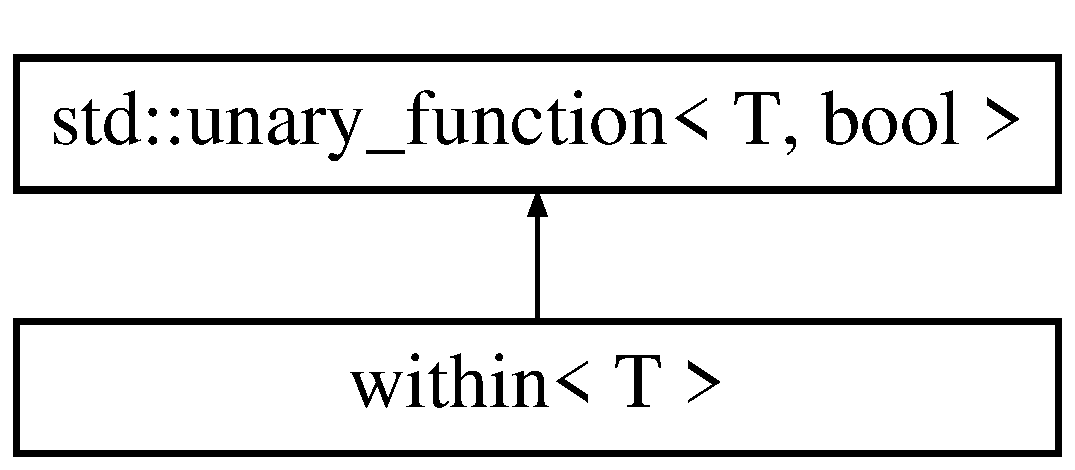
\includegraphics[height=2.000000cm]{classwithin}
\end{center}
\end{figure}
\subsection*{Public Member Functions}
\begin{DoxyCompactItemize}
\item 
\hypertarget{classwithin_ac461f80eef6cbe70a69729fd5b99f751}{{\bfseries within} (T range\-\_\-begin, T range\-\_\-end)}\label{classwithin_ac461f80eef6cbe70a69729fd5b99f751}

\item 
\hypertarget{classwithin_aaab5ecca0235613f499bc5e607d23cbd}{bool {\bfseries operator()} (T value) const }\label{classwithin_aaab5ecca0235613f499bc5e607d23cbd}

\end{DoxyCompactItemize}


\subsection{Detailed Description}
\subsubsection*{template$<$typename T$>$class within$<$ T $>$}

determines if a value is within a given range 

The documentation for this class was generated from the following file\-:\begin{DoxyCompactItemize}
\item 
utilities/utilities.\-h\end{DoxyCompactItemize}

\hypertarget{classrapidxml_1_1xml__attribute}{\section{rapidxml\-:\-:xml\-\_\-attribute$<$ Ch $>$ Class Template Reference}
\label{classrapidxml_1_1xml__attribute}\index{rapidxml\-::xml\-\_\-attribute$<$ Ch $>$@{rapidxml\-::xml\-\_\-attribute$<$ Ch $>$}}
}


{\ttfamily \#include $<$rapidxml.\-hpp$>$}

Inheritance diagram for rapidxml\-:\-:xml\-\_\-attribute$<$ Ch $>$\-:\begin{figure}[H]
\begin{center}
\leavevmode
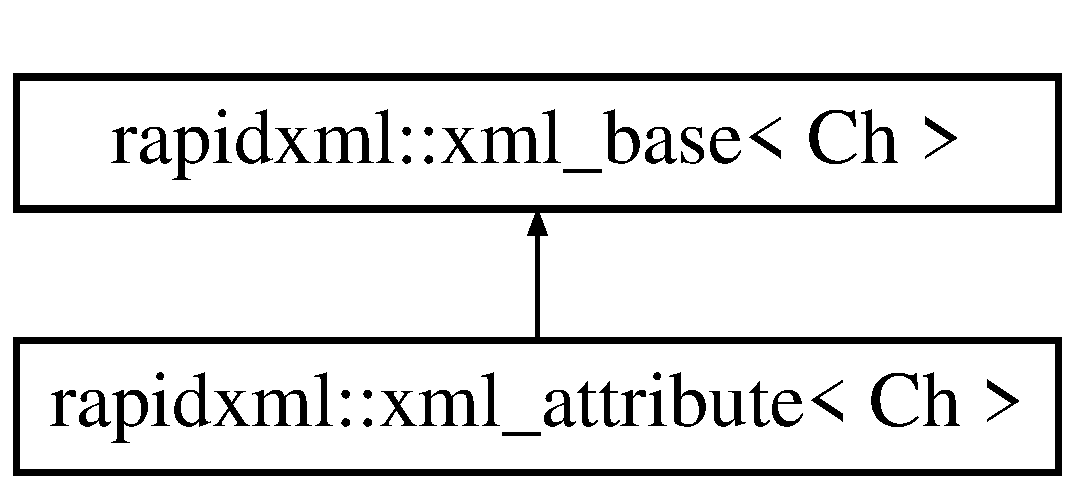
\includegraphics[height=2.000000cm]{classrapidxml_1_1xml__attribute}
\end{center}
\end{figure}
\subsection*{Public Member Functions}
\begin{DoxyCompactItemize}
\item 
\hyperlink{classrapidxml_1_1xml__attribute_a26be291103917d3e8de110d46dd83816}{xml\-\_\-attribute} ()
\item 
\hyperlink{classrapidxml_1_1xml__document}{xml\-\_\-document}$<$ Ch $>$ $\ast$ \hyperlink{classrapidxml_1_1xml__attribute_a8b6d31d899e27f01bde35b53d98496ec}{document} () const 
\item 
\hyperlink{classrapidxml_1_1xml__attribute}{xml\-\_\-attribute}$<$ Ch $>$ $\ast$ \hyperlink{classrapidxml_1_1xml__attribute_ae3547cc30b201fd6d7b98c04dda26f89}{previous\-\_\-attribute} (const Ch $\ast$\hyperlink{classrapidxml_1_1xml__base_a9a09739310469995db078ebd0da3ed45}{name}=0, std\-::size\-\_\-t \hyperlink{classrapidxml_1_1xml__base_a7e7f98b3d01e1eab8dc1ca69aad9af84}{name\-\_\-size}=0, bool case\-\_\-sensitive=true) const 
\item 
\hyperlink{classrapidxml_1_1xml__attribute}{xml\-\_\-attribute}$<$ Ch $>$ $\ast$ \hyperlink{classrapidxml_1_1xml__attribute_a56c08d7c96203286c889a43849328a86}{next\-\_\-attribute} (const Ch $\ast$\hyperlink{classrapidxml_1_1xml__base_a9a09739310469995db078ebd0da3ed45}{name}=0, std\-::size\-\_\-t \hyperlink{classrapidxml_1_1xml__base_a7e7f98b3d01e1eab8dc1ca69aad9af84}{name\-\_\-size}=0, bool case\-\_\-sensitive=true) const 
\end{DoxyCompactItemize}
\subsection*{Friends}
\begin{DoxyCompactItemize}
\item 
\hypertarget{classrapidxml_1_1xml__attribute_aa7e464ce3fe512598ff8dda47291941f}{class {\bfseries xml\-\_\-node$<$ Ch $>$}}\label{classrapidxml_1_1xml__attribute_aa7e464ce3fe512598ff8dda47291941f}

\end{DoxyCompactItemize}
\subsection*{Additional Inherited Members}


\subsection{Detailed Description}
\subsubsection*{template$<$class Ch$>$class rapidxml\-::xml\-\_\-attribute$<$ Ch $>$}

Class representing attribute node of X\-M\-L document. Each attribute has name and value strings, which are available through \hyperlink{classrapidxml_1_1xml__base_a9a09739310469995db078ebd0da3ed45}{name()} and \hyperlink{classrapidxml_1_1xml__base_adcdaccff61c665f039d9344e447b7445}{value()} functions (inherited from \hyperlink{classrapidxml_1_1xml__base}{xml\-\_\-base}). Note that after parse, both name and value of attribute will point to interior of source text used for parsing. Thus, this text must persist in memory for the lifetime of attribute. 
\begin{DoxyParams}{Parameters}
{\em Ch} & Character type to use. \\
\hline
\end{DoxyParams}


\subsection{Constructor \& Destructor Documentation}
\hypertarget{classrapidxml_1_1xml__attribute_a26be291103917d3e8de110d46dd83816}{\index{rapidxml\-::xml\-\_\-attribute@{rapidxml\-::xml\-\_\-attribute}!xml\-\_\-attribute@{xml\-\_\-attribute}}
\index{xml\-\_\-attribute@{xml\-\_\-attribute}!rapidxml::xml_attribute@{rapidxml\-::xml\-\_\-attribute}}
\subsubsection[{xml\-\_\-attribute}]{\setlength{\rightskip}{0pt plus 5cm}template$<$class Ch$>$ {\bf rapidxml\-::xml\-\_\-attribute}$<$ Ch $>$\-::{\bf xml\-\_\-attribute} (
\begin{DoxyParamCaption}
{}
\end{DoxyParamCaption}
)\hspace{0.3cm}{\ttfamily [inline]}}}\label{classrapidxml_1_1xml__attribute_a26be291103917d3e8de110d46dd83816}
Constructs an empty attribute with the specified type. Consider using \hyperlink{classrapidxml_1_1memory__pool}{memory\-\_\-pool} of appropriate \hyperlink{classrapidxml_1_1xml__document}{xml\-\_\-document} if allocating attributes manually. 

\subsection{Member Function Documentation}
\hypertarget{classrapidxml_1_1xml__attribute_a8b6d31d899e27f01bde35b53d98496ec}{\index{rapidxml\-::xml\-\_\-attribute@{rapidxml\-::xml\-\_\-attribute}!document@{document}}
\index{document@{document}!rapidxml::xml_attribute@{rapidxml\-::xml\-\_\-attribute}}
\subsubsection[{document}]{\setlength{\rightskip}{0pt plus 5cm}template$<$class Ch$>$ {\bf xml\-\_\-document}$<$Ch$>$$\ast$ {\bf rapidxml\-::xml\-\_\-attribute}$<$ Ch $>$\-::document (
\begin{DoxyParamCaption}
{}
\end{DoxyParamCaption}
) const\hspace{0.3cm}{\ttfamily [inline]}}}\label{classrapidxml_1_1xml__attribute_a8b6d31d899e27f01bde35b53d98496ec}
Gets document of which attribute is a child. \begin{DoxyReturn}{Returns}
Pointer to document that contains this attribute, or 0 if there is no parent document. 
\end{DoxyReturn}
\hypertarget{classrapidxml_1_1xml__attribute_a56c08d7c96203286c889a43849328a86}{\index{rapidxml\-::xml\-\_\-attribute@{rapidxml\-::xml\-\_\-attribute}!next\-\_\-attribute@{next\-\_\-attribute}}
\index{next\-\_\-attribute@{next\-\_\-attribute}!rapidxml::xml_attribute@{rapidxml\-::xml\-\_\-attribute}}
\subsubsection[{next\-\_\-attribute}]{\setlength{\rightskip}{0pt plus 5cm}template$<$class Ch$>$ {\bf xml\-\_\-attribute}$<$Ch$>$$\ast$ {\bf rapidxml\-::xml\-\_\-attribute}$<$ Ch $>$\-::next\-\_\-attribute (
\begin{DoxyParamCaption}
\item[{const Ch $\ast$}]{name = {\ttfamily 0}, }
\item[{std\-::size\-\_\-t}]{name\-\_\-size = {\ttfamily 0}, }
\item[{bool}]{case\-\_\-sensitive = {\ttfamily true}}
\end{DoxyParamCaption}
) const\hspace{0.3cm}{\ttfamily [inline]}}}\label{classrapidxml_1_1xml__attribute_a56c08d7c96203286c889a43849328a86}
Gets next attribute, optionally matching attribute name. 
\begin{DoxyParams}{Parameters}
{\em name} & Name of attribute to find, or 0 to return next attribute regardless of its name; this string doesn't have to be zero-\/terminated if name\-\_\-size is non-\/zero \\
\hline
{\em name\-\_\-size} & Size of name, in characters, or 0 to have size calculated automatically from string \\
\hline
{\em case\-\_\-sensitive} & Should name comparison be case-\/sensitive; non case-\/sensitive comparison works properly only for A\-S\-C\-I\-I characters \\
\hline
\end{DoxyParams}
\begin{DoxyReturn}{Returns}
Pointer to found attribute, or 0 if not found. 
\end{DoxyReturn}
\hypertarget{classrapidxml_1_1xml__attribute_ae3547cc30b201fd6d7b98c04dda26f89}{\index{rapidxml\-::xml\-\_\-attribute@{rapidxml\-::xml\-\_\-attribute}!previous\-\_\-attribute@{previous\-\_\-attribute}}
\index{previous\-\_\-attribute@{previous\-\_\-attribute}!rapidxml::xml_attribute@{rapidxml\-::xml\-\_\-attribute}}
\subsubsection[{previous\-\_\-attribute}]{\setlength{\rightskip}{0pt plus 5cm}template$<$class Ch$>$ {\bf xml\-\_\-attribute}$<$Ch$>$$\ast$ {\bf rapidxml\-::xml\-\_\-attribute}$<$ Ch $>$\-::previous\-\_\-attribute (
\begin{DoxyParamCaption}
\item[{const Ch $\ast$}]{name = {\ttfamily 0}, }
\item[{std\-::size\-\_\-t}]{name\-\_\-size = {\ttfamily 0}, }
\item[{bool}]{case\-\_\-sensitive = {\ttfamily true}}
\end{DoxyParamCaption}
) const\hspace{0.3cm}{\ttfamily [inline]}}}\label{classrapidxml_1_1xml__attribute_ae3547cc30b201fd6d7b98c04dda26f89}
Gets previous attribute, optionally matching attribute name. 
\begin{DoxyParams}{Parameters}
{\em name} & Name of attribute to find, or 0 to return previous attribute regardless of its name; this string doesn't have to be zero-\/terminated if name\-\_\-size is non-\/zero \\
\hline
{\em name\-\_\-size} & Size of name, in characters, or 0 to have size calculated automatically from string \\
\hline
{\em case\-\_\-sensitive} & Should name comparison be case-\/sensitive; non case-\/sensitive comparison works properly only for A\-S\-C\-I\-I characters \\
\hline
\end{DoxyParams}
\begin{DoxyReturn}{Returns}
Pointer to found attribute, or 0 if not found. 
\end{DoxyReturn}


The documentation for this class was generated from the following file\-:\begin{DoxyCompactItemize}
\item 
rapidxml/\hyperlink{rapidxml_8hpp}{rapidxml.\-hpp}\end{DoxyCompactItemize}

\hypertarget{classrapidxml_1_1xml__base}{\section{rapidxml\-:\-:xml\-\_\-base$<$ Ch $>$ Class Template Reference}
\label{classrapidxml_1_1xml__base}\index{rapidxml\-::xml\-\_\-base$<$ Ch $>$@{rapidxml\-::xml\-\_\-base$<$ Ch $>$}}
}


{\ttfamily \#include $<$rapidxml.\-hpp$>$}

Inheritance diagram for rapidxml\-:\-:xml\-\_\-base$<$ Ch $>$\-:\begin{figure}[H]
\begin{center}
\leavevmode
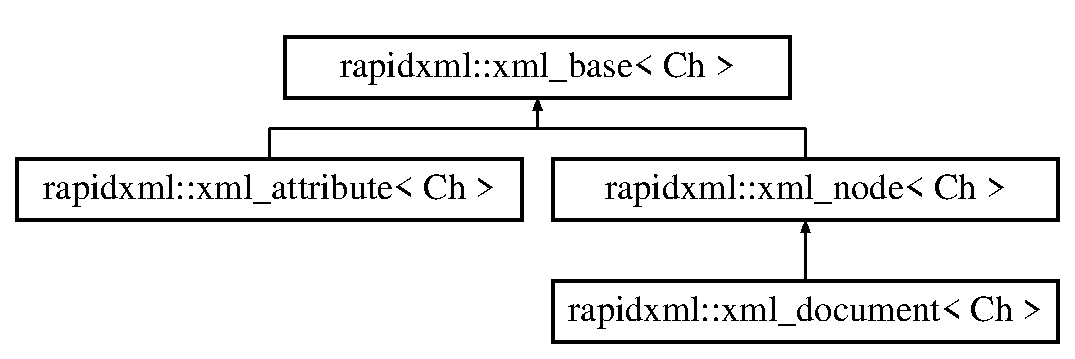
\includegraphics[height=3.000000cm]{classrapidxml_1_1xml__base}
\end{center}
\end{figure}
\subsection*{Public Member Functions}
\begin{DoxyCompactItemize}
\item 
Ch $\ast$ \hyperlink{classrapidxml_1_1xml__base_a9a09739310469995db078ebd0da3ed45}{name} () const 
\item 
std\-::size\-\_\-t \hyperlink{classrapidxml_1_1xml__base_a7e7f98b3d01e1eab8dc1ca69aad9af84}{name\-\_\-size} () const 
\item 
Ch $\ast$ \hyperlink{classrapidxml_1_1xml__base_adcdaccff61c665f039d9344e447b7445}{value} () const 
\item 
std\-::size\-\_\-t \hyperlink{classrapidxml_1_1xml__base_a9fcf201ed0915ac18dd43b0b5dcfaf32}{value\-\_\-size} () const 
\item 
void \hyperlink{classrapidxml_1_1xml__base_ae55060ae958c6e6465d6c8db852ec6ce}{name} (const Ch $\ast$name, std\-::size\-\_\-t size)
\item 
void \hyperlink{classrapidxml_1_1xml__base_a4611ddc82ac83a527c65606600eb2a0d}{name} (const Ch $\ast$name)
\item 
void \hyperlink{classrapidxml_1_1xml__base_a3b183c2db7022a6d30494dd2f0ac11e9}{value} (const Ch $\ast$value, std\-::size\-\_\-t size)
\item 
void \hyperlink{classrapidxml_1_1xml__base_a81e63ec4bfd2d7ef0a6c2ed49be6e623}{value} (const Ch $\ast$value)
\item 
\hyperlink{classrapidxml_1_1xml__node}{xml\-\_\-node}$<$ Ch $>$ $\ast$ \hyperlink{classrapidxml_1_1xml__base_a7f31ae930f93852830234db1ae59c4c4}{parent} () const 
\end{DoxyCompactItemize}
\subsection*{Static Protected Member Functions}
\begin{DoxyCompactItemize}
\item 
\hypertarget{classrapidxml_1_1xml__base_ad96ff6b1e41dab3ff60b9bc4df769a75}{static Ch $\ast$ {\bfseries nullstr} ()}\label{classrapidxml_1_1xml__base_ad96ff6b1e41dab3ff60b9bc4df769a75}

\end{DoxyCompactItemize}
\subsection*{Protected Attributes}
\begin{DoxyCompactItemize}
\item 
\hypertarget{classrapidxml_1_1xml__base_afd9851ed43e14619db0d7075ef8e9e8a}{Ch $\ast$ {\bfseries m\-\_\-name}}\label{classrapidxml_1_1xml__base_afd9851ed43e14619db0d7075ef8e9e8a}

\item 
\hypertarget{classrapidxml_1_1xml__base_a278a1ea63b0b70219b946cec47fa00ea}{Ch $\ast$ {\bfseries m\-\_\-value}}\label{classrapidxml_1_1xml__base_a278a1ea63b0b70219b946cec47fa00ea}

\item 
\hypertarget{classrapidxml_1_1xml__base_a5a8c76a7274b4180213796422c4df76f}{std\-::size\-\_\-t {\bfseries m\-\_\-name\-\_\-size}}\label{classrapidxml_1_1xml__base_a5a8c76a7274b4180213796422c4df76f}

\item 
\hypertarget{classrapidxml_1_1xml__base_aa3a49d8ceddb8a8d7edb773a2226b89c}{std\-::size\-\_\-t {\bfseries m\-\_\-value\-\_\-size}}\label{classrapidxml_1_1xml__base_aa3a49d8ceddb8a8d7edb773a2226b89c}

\item 
\hypertarget{classrapidxml_1_1xml__base_a90d5f660f078f66563fd7b2d8387ccb0}{\hyperlink{classrapidxml_1_1xml__node}{xml\-\_\-node}$<$ Ch $>$ $\ast$ {\bfseries m\-\_\-parent}}\label{classrapidxml_1_1xml__base_a90d5f660f078f66563fd7b2d8387ccb0}

\end{DoxyCompactItemize}


\subsection{Detailed Description}
\subsubsection*{template$<$class Ch = char$>$class rapidxml\-::xml\-\_\-base$<$ Ch $>$}

Base class for \hyperlink{classrapidxml_1_1xml__node}{xml\-\_\-node} and \hyperlink{classrapidxml_1_1xml__attribute}{xml\-\_\-attribute} implementing common functions\-: \hyperlink{classrapidxml_1_1xml__base_a9a09739310469995db078ebd0da3ed45}{name()}, \hyperlink{classrapidxml_1_1xml__base_a7e7f98b3d01e1eab8dc1ca69aad9af84}{name\-\_\-size()}, \hyperlink{classrapidxml_1_1xml__base_adcdaccff61c665f039d9344e447b7445}{value()}, \hyperlink{classrapidxml_1_1xml__base_a9fcf201ed0915ac18dd43b0b5dcfaf32}{value\-\_\-size()} and \hyperlink{classrapidxml_1_1xml__base_a7f31ae930f93852830234db1ae59c4c4}{parent()}. 
\begin{DoxyParams}{Parameters}
{\em Ch} & Character type to use \\
\hline
\end{DoxyParams}


\subsection{Member Function Documentation}
\hypertarget{classrapidxml_1_1xml__base_a9a09739310469995db078ebd0da3ed45}{\index{rapidxml\-::xml\-\_\-base@{rapidxml\-::xml\-\_\-base}!name@{name}}
\index{name@{name}!rapidxml::xml_base@{rapidxml\-::xml\-\_\-base}}
\subsubsection[{name}]{\setlength{\rightskip}{0pt plus 5cm}template$<$class Ch  = char$>$ Ch$\ast$ {\bf rapidxml\-::xml\-\_\-base}$<$ Ch $>$\-::name (
\begin{DoxyParamCaption}
{}
\end{DoxyParamCaption}
) const\hspace{0.3cm}{\ttfamily [inline]}}}\label{classrapidxml_1_1xml__base_a9a09739310469995db078ebd0da3ed45}
Gets name of the node. Interpretation of name depends on type of node. Note that name will not be zero-\/terminated if rapidxml\-::parse\-\_\-no\-\_\-string\-\_\-terminators option was selected during parse. \par
\par
 Use \hyperlink{classrapidxml_1_1xml__base_a7e7f98b3d01e1eab8dc1ca69aad9af84}{name\-\_\-size()} function to determine length of the name. \begin{DoxyReturn}{Returns}
Name of node, or empty string if node has no name. 
\end{DoxyReturn}
\hypertarget{classrapidxml_1_1xml__base_ae55060ae958c6e6465d6c8db852ec6ce}{\index{rapidxml\-::xml\-\_\-base@{rapidxml\-::xml\-\_\-base}!name@{name}}
\index{name@{name}!rapidxml::xml_base@{rapidxml\-::xml\-\_\-base}}
\subsubsection[{name}]{\setlength{\rightskip}{0pt plus 5cm}template$<$class Ch  = char$>$ void {\bf rapidxml\-::xml\-\_\-base}$<$ Ch $>$\-::name (
\begin{DoxyParamCaption}
\item[{const Ch $\ast$}]{name, }
\item[{std\-::size\-\_\-t}]{size}
\end{DoxyParamCaption}
)\hspace{0.3cm}{\ttfamily [inline]}}}\label{classrapidxml_1_1xml__base_ae55060ae958c6e6465d6c8db852ec6ce}
Sets name of node to a non zero-\/terminated string. See ownership\-\_\-of\-\_\-strings. \par
\par
 Note that node does not own its name or value, it only stores a pointer to it. It will not delete or otherwise free the pointer on destruction. It is reponsibility of the user to properly manage lifetime of the string. The easiest way to achieve it is to use \hyperlink{classrapidxml_1_1memory__pool}{memory\-\_\-pool} of the document to allocate the string -\/ on destruction of the document the string will be automatically freed. \par
\par
 Size of name must be specified separately, because name does not have to be zero terminated. Use \hyperlink{classrapidxml_1_1xml__base_a4611ddc82ac83a527c65606600eb2a0d}{name(const Ch $\ast$)} function to have the length automatically calculated (string must be zero terminated). 
\begin{DoxyParams}{Parameters}
{\em name} & Name of node to set. Does not have to be zero terminated. \\
\hline
{\em size} & Size of name, in characters. This does not include zero terminator, if one is present. \\
\hline
\end{DoxyParams}
\hypertarget{classrapidxml_1_1xml__base_a4611ddc82ac83a527c65606600eb2a0d}{\index{rapidxml\-::xml\-\_\-base@{rapidxml\-::xml\-\_\-base}!name@{name}}
\index{name@{name}!rapidxml::xml_base@{rapidxml\-::xml\-\_\-base}}
\subsubsection[{name}]{\setlength{\rightskip}{0pt plus 5cm}template$<$class Ch  = char$>$ void {\bf rapidxml\-::xml\-\_\-base}$<$ Ch $>$\-::name (
\begin{DoxyParamCaption}
\item[{const Ch $\ast$}]{name}
\end{DoxyParamCaption}
)\hspace{0.3cm}{\ttfamily [inline]}}}\label{classrapidxml_1_1xml__base_a4611ddc82ac83a527c65606600eb2a0d}
Sets name of node to a zero-\/terminated string. See also ownership\-\_\-of\-\_\-strings and \hyperlink{classrapidxml_1_1xml__base_ae55060ae958c6e6465d6c8db852ec6ce}{xml\-\_\-node\-::name(const Ch $\ast$, std\-::size\-\_\-t)}. 
\begin{DoxyParams}{Parameters}
{\em name} & Name of node to set. Must be zero terminated. \\
\hline
\end{DoxyParams}
\hypertarget{classrapidxml_1_1xml__base_a7e7f98b3d01e1eab8dc1ca69aad9af84}{\index{rapidxml\-::xml\-\_\-base@{rapidxml\-::xml\-\_\-base}!name\-\_\-size@{name\-\_\-size}}
\index{name\-\_\-size@{name\-\_\-size}!rapidxml::xml_base@{rapidxml\-::xml\-\_\-base}}
\subsubsection[{name\-\_\-size}]{\setlength{\rightskip}{0pt plus 5cm}template$<$class Ch  = char$>$ std\-::size\-\_\-t {\bf rapidxml\-::xml\-\_\-base}$<$ Ch $>$\-::name\-\_\-size (
\begin{DoxyParamCaption}
{}
\end{DoxyParamCaption}
) const\hspace{0.3cm}{\ttfamily [inline]}}}\label{classrapidxml_1_1xml__base_a7e7f98b3d01e1eab8dc1ca69aad9af84}
Gets size of node name, not including terminator character. This function works correctly irrespective of whether name is or is not zero terminated. \begin{DoxyReturn}{Returns}
Size of node name, in characters. 
\end{DoxyReturn}
\hypertarget{classrapidxml_1_1xml__base_a7f31ae930f93852830234db1ae59c4c4}{\index{rapidxml\-::xml\-\_\-base@{rapidxml\-::xml\-\_\-base}!parent@{parent}}
\index{parent@{parent}!rapidxml::xml_base@{rapidxml\-::xml\-\_\-base}}
\subsubsection[{parent}]{\setlength{\rightskip}{0pt plus 5cm}template$<$class Ch  = char$>$ {\bf xml\-\_\-node}$<$Ch$>$$\ast$ {\bf rapidxml\-::xml\-\_\-base}$<$ Ch $>$\-::parent (
\begin{DoxyParamCaption}
{}
\end{DoxyParamCaption}
) const\hspace{0.3cm}{\ttfamily [inline]}}}\label{classrapidxml_1_1xml__base_a7f31ae930f93852830234db1ae59c4c4}
Gets node parent. \begin{DoxyReturn}{Returns}
Pointer to parent node, or 0 if there is no parent. 
\end{DoxyReturn}
\hypertarget{classrapidxml_1_1xml__base_adcdaccff61c665f039d9344e447b7445}{\index{rapidxml\-::xml\-\_\-base@{rapidxml\-::xml\-\_\-base}!value@{value}}
\index{value@{value}!rapidxml::xml_base@{rapidxml\-::xml\-\_\-base}}
\subsubsection[{value}]{\setlength{\rightskip}{0pt plus 5cm}template$<$class Ch  = char$>$ Ch$\ast$ {\bf rapidxml\-::xml\-\_\-base}$<$ Ch $>$\-::value (
\begin{DoxyParamCaption}
{}
\end{DoxyParamCaption}
) const\hspace{0.3cm}{\ttfamily [inline]}}}\label{classrapidxml_1_1xml__base_adcdaccff61c665f039d9344e447b7445}
Gets value of node. Interpretation of value depends on type of node. Note that value will not be zero-\/terminated if rapidxml\-::parse\-\_\-no\-\_\-string\-\_\-terminators option was selected during parse. \par
\par
 Use \hyperlink{classrapidxml_1_1xml__base_a9fcf201ed0915ac18dd43b0b5dcfaf32}{value\-\_\-size()} function to determine length of the value. \begin{DoxyReturn}{Returns}
Value of node, or empty string if node has no value. 
\end{DoxyReturn}
\hypertarget{classrapidxml_1_1xml__base_a3b183c2db7022a6d30494dd2f0ac11e9}{\index{rapidxml\-::xml\-\_\-base@{rapidxml\-::xml\-\_\-base}!value@{value}}
\index{value@{value}!rapidxml::xml_base@{rapidxml\-::xml\-\_\-base}}
\subsubsection[{value}]{\setlength{\rightskip}{0pt plus 5cm}template$<$class Ch  = char$>$ void {\bf rapidxml\-::xml\-\_\-base}$<$ Ch $>$\-::value (
\begin{DoxyParamCaption}
\item[{const Ch $\ast$}]{value, }
\item[{std\-::size\-\_\-t}]{size}
\end{DoxyParamCaption}
)\hspace{0.3cm}{\ttfamily [inline]}}}\label{classrapidxml_1_1xml__base_a3b183c2db7022a6d30494dd2f0ac11e9}
Sets value of node to a non zero-\/terminated string. See ownership\-\_\-of\-\_\-strings. \par
\par
 Note that node does not own its name or value, it only stores a pointer to it. It will not delete or otherwise free the pointer on destruction. It is reponsibility of the user to properly manage lifetime of the string. The easiest way to achieve it is to use \hyperlink{classrapidxml_1_1memory__pool}{memory\-\_\-pool} of the document to allocate the string -\/ on destruction of the document the string will be automatically freed. \par
\par
 Size of value must be specified separately, because it does not have to be zero terminated. Use \hyperlink{classrapidxml_1_1xml__base_a81e63ec4bfd2d7ef0a6c2ed49be6e623}{value(const Ch $\ast$)} function to have the length automatically calculated (string must be zero terminated). \par
\par
 If an element has a child node of type node\-\_\-data, it will take precedence over element value when printing. If you want to manipulate data of elements using values, use parser flag rapidxml\-::parse\-\_\-no\-\_\-data\-\_\-nodes to prevent creation of data nodes by the parser. 
\begin{DoxyParams}{Parameters}
{\em value} & value of node to set. Does not have to be zero terminated. \\
\hline
{\em size} & Size of value, in characters. This does not include zero terminator, if one is present. \\
\hline
\end{DoxyParams}
\hypertarget{classrapidxml_1_1xml__base_a81e63ec4bfd2d7ef0a6c2ed49be6e623}{\index{rapidxml\-::xml\-\_\-base@{rapidxml\-::xml\-\_\-base}!value@{value}}
\index{value@{value}!rapidxml::xml_base@{rapidxml\-::xml\-\_\-base}}
\subsubsection[{value}]{\setlength{\rightskip}{0pt plus 5cm}template$<$class Ch  = char$>$ void {\bf rapidxml\-::xml\-\_\-base}$<$ Ch $>$\-::value (
\begin{DoxyParamCaption}
\item[{const Ch $\ast$}]{value}
\end{DoxyParamCaption}
)\hspace{0.3cm}{\ttfamily [inline]}}}\label{classrapidxml_1_1xml__base_a81e63ec4bfd2d7ef0a6c2ed49be6e623}
Sets value of node to a zero-\/terminated string. See also ownership\-\_\-of\-\_\-strings and \hyperlink{classrapidxml_1_1xml__base_a3b183c2db7022a6d30494dd2f0ac11e9}{xml\-\_\-node\-::value(const Ch $\ast$, std\-::size\-\_\-t)}. 
\begin{DoxyParams}{Parameters}
{\em value} & Vame of node to set. Must be zero terminated. \\
\hline
\end{DoxyParams}
\hypertarget{classrapidxml_1_1xml__base_a9fcf201ed0915ac18dd43b0b5dcfaf32}{\index{rapidxml\-::xml\-\_\-base@{rapidxml\-::xml\-\_\-base}!value\-\_\-size@{value\-\_\-size}}
\index{value\-\_\-size@{value\-\_\-size}!rapidxml::xml_base@{rapidxml\-::xml\-\_\-base}}
\subsubsection[{value\-\_\-size}]{\setlength{\rightskip}{0pt plus 5cm}template$<$class Ch  = char$>$ std\-::size\-\_\-t {\bf rapidxml\-::xml\-\_\-base}$<$ Ch $>$\-::value\-\_\-size (
\begin{DoxyParamCaption}
{}
\end{DoxyParamCaption}
) const\hspace{0.3cm}{\ttfamily [inline]}}}\label{classrapidxml_1_1xml__base_a9fcf201ed0915ac18dd43b0b5dcfaf32}
Gets size of node value, not including terminator character. This function works correctly irrespective of whether value is or is not zero terminated. \begin{DoxyReturn}{Returns}
Size of node value, in characters. 
\end{DoxyReturn}


The documentation for this class was generated from the following file\-:\begin{DoxyCompactItemize}
\item 
rapidxml/\hyperlink{rapidxml_8hpp}{rapidxml.\-hpp}\end{DoxyCompactItemize}

\hypertarget{classrapidxml_1_1xml__document}{\section{rapidxml\-:\-:xml\-\_\-document$<$ Ch $>$ Class Template Reference}
\label{classrapidxml_1_1xml__document}\index{rapidxml\-::xml\-\_\-document$<$ Ch $>$@{rapidxml\-::xml\-\_\-document$<$ Ch $>$}}
}


{\ttfamily \#include $<$rapidxml.\-hpp$>$}

Inheritance diagram for rapidxml\-:\-:xml\-\_\-document$<$ Ch $>$\-:\begin{figure}[H]
\begin{center}
\leavevmode
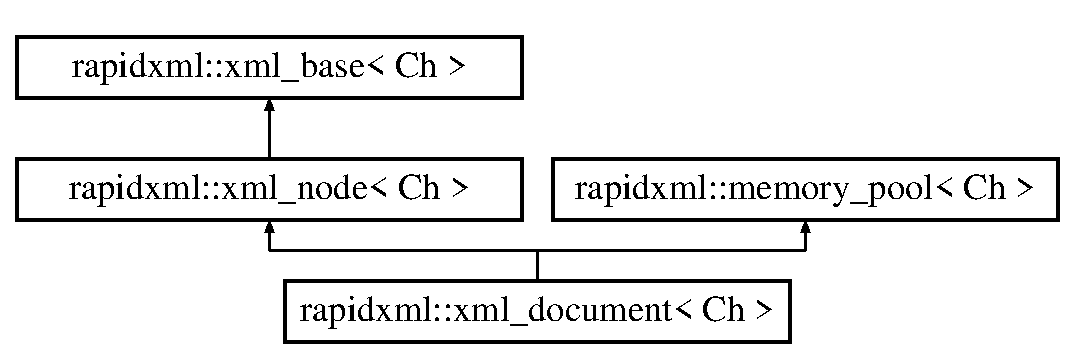
\includegraphics[height=3.000000cm]{classrapidxml_1_1xml__document}
\end{center}
\end{figure}
\subsection*{Public Member Functions}
\begin{DoxyCompactItemize}
\item 
\hypertarget{classrapidxml_1_1xml__document_aae8841b15085ba8f32ff46587ace28f5}{\hyperlink{classrapidxml_1_1xml__document_aae8841b15085ba8f32ff46587ace28f5}{xml\-\_\-document} ()}\label{classrapidxml_1_1xml__document_aae8841b15085ba8f32ff46587ace28f5}

\begin{DoxyCompactList}\small\item\em Constructs empty X\-M\-L document. \end{DoxyCompactList}\item 
{\footnotesize template$<$int Flags$>$ }\\void \hyperlink{classrapidxml_1_1xml__document_ac6e73ff9ac323bf5a370c38feb03a6b1}{parse} (Ch $\ast$text)
\item 
void \hyperlink{classrapidxml_1_1xml__document_a826929ff54242532198701f19ff5f83f}{clear} ()
\end{DoxyCompactItemize}
\subsection*{Additional Inherited Members}


\subsection{Detailed Description}
\subsubsection*{template$<$class Ch$>$class rapidxml\-::xml\-\_\-document$<$ Ch $>$}

This class represents root of the D\-O\-M hierarchy. It is also an \hyperlink{classrapidxml_1_1xml__node}{xml\-\_\-node} and a \hyperlink{classrapidxml_1_1memory__pool}{memory\-\_\-pool} through public inheritance. Use \hyperlink{classrapidxml_1_1xml__document_ac6e73ff9ac323bf5a370c38feb03a6b1}{parse()} function to build a D\-O\-M tree from a zero-\/terminated X\-M\-L text string. \hyperlink{classrapidxml_1_1xml__document_ac6e73ff9ac323bf5a370c38feb03a6b1}{parse()} function allocates memory for nodes and attributes by using functions of \hyperlink{classrapidxml_1_1xml__document}{xml\-\_\-document}, which are inherited from \hyperlink{classrapidxml_1_1memory__pool}{memory\-\_\-pool}. To access root node of the document, use the document itself, as if it was an \hyperlink{classrapidxml_1_1xml__node}{xml\-\_\-node}. 
\begin{DoxyParams}{Parameters}
{\em Ch} & Character type to use. \\
\hline
\end{DoxyParams}


\subsection{Member Function Documentation}
\hypertarget{classrapidxml_1_1xml__document_a826929ff54242532198701f19ff5f83f}{\index{rapidxml\-::xml\-\_\-document@{rapidxml\-::xml\-\_\-document}!clear@{clear}}
\index{clear@{clear}!rapidxml::xml_document@{rapidxml\-::xml\-\_\-document}}
\subsubsection[{clear}]{\setlength{\rightskip}{0pt plus 5cm}template$<$class Ch $>$ void {\bf rapidxml\-::xml\-\_\-document}$<$ Ch $>$\-::clear (
\begin{DoxyParamCaption}
{}
\end{DoxyParamCaption}
)\hspace{0.3cm}{\ttfamily [inline]}}}\label{classrapidxml_1_1xml__document_a826929ff54242532198701f19ff5f83f}
Clears the document by deleting all nodes and clearing the memory pool. All nodes owned by document pool are destroyed. \hypertarget{classrapidxml_1_1xml__document_ac6e73ff9ac323bf5a370c38feb03a6b1}{\index{rapidxml\-::xml\-\_\-document@{rapidxml\-::xml\-\_\-document}!parse@{parse}}
\index{parse@{parse}!rapidxml::xml_document@{rapidxml\-::xml\-\_\-document}}
\subsubsection[{parse}]{\setlength{\rightskip}{0pt plus 5cm}template$<$class Ch $>$ template$<$int Flags$>$ void {\bf rapidxml\-::xml\-\_\-document}$<$ Ch $>$\-::parse (
\begin{DoxyParamCaption}
\item[{Ch $\ast$}]{text}
\end{DoxyParamCaption}
)\hspace{0.3cm}{\ttfamily [inline]}}}\label{classrapidxml_1_1xml__document_ac6e73ff9ac323bf5a370c38feb03a6b1}
Parses zero-\/terminated X\-M\-L string according to given flags. Passed string will be modified by the parser, unless rapidxml\-::parse\-\_\-non\-\_\-destructive flag is used. The string must persist for the lifetime of the document. In case of error, \hyperlink{classrapidxml_1_1parse__error}{rapidxml\-::parse\-\_\-error} exception will be thrown. \par
\par
 If you want to parse contents of a file, you must first load the file into the memory, and pass pointer to its beginning. Make sure that data is zero-\/terminated. \par
\par
 Document can be parsed into multiple times. Each new call to parse removes previous nodes and attributes (if any), but does not clear memory pool. 
\begin{DoxyParams}{Parameters}
{\em text} & X\-M\-L data to parse; pointer is non-\/const to denote fact that this data may be modified by the parser. \\
\hline
\end{DoxyParams}


The documentation for this class was generated from the following file\-:\begin{DoxyCompactItemize}
\item 
rapidxml/\hyperlink{rapidxml_8hpp}{rapidxml.\-hpp}\end{DoxyCompactItemize}

\hypertarget{classrapidxml_1_1xml__node}{\section{rapidxml\-:\-:xml\-\_\-node$<$ Ch $>$ Class Template Reference}
\label{classrapidxml_1_1xml__node}\index{rapidxml\-::xml\-\_\-node$<$ Ch $>$@{rapidxml\-::xml\-\_\-node$<$ Ch $>$}}
}


{\ttfamily \#include $<$rapidxml.\-hpp$>$}

Inheritance diagram for rapidxml\-:\-:xml\-\_\-node$<$ Ch $>$\-:\begin{figure}[H]
\begin{center}
\leavevmode
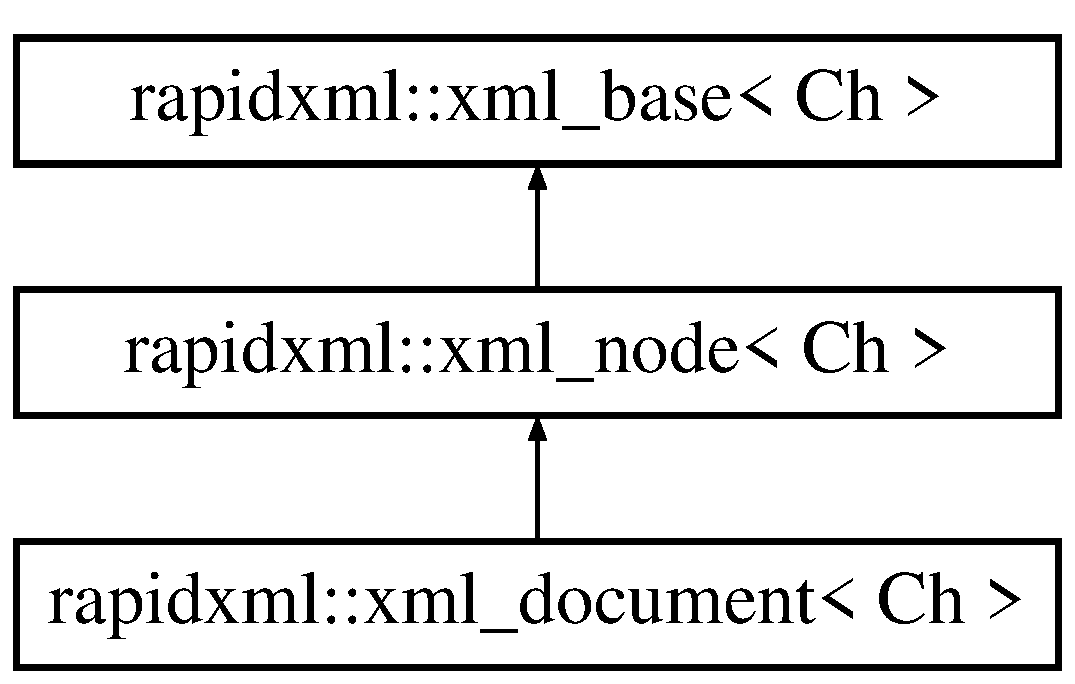
\includegraphics[height=3.000000cm]{classrapidxml_1_1xml__node}
\end{center}
\end{figure}
\subsection*{Public Member Functions}
\begin{DoxyCompactItemize}
\item 
\hyperlink{classrapidxml_1_1xml__node_a8bd9019960b90605a45998b661fb1b0e}{xml\-\_\-node} (node\-\_\-type \hyperlink{classrapidxml_1_1xml__node_a2c6a4315b98bcfa2e04fed3fa1b22c36}{type})
\item 
node\-\_\-type \hyperlink{classrapidxml_1_1xml__node_a2c6a4315b98bcfa2e04fed3fa1b22c36}{type} () const 
\item 
\hyperlink{classrapidxml_1_1xml__document}{xml\-\_\-document}$<$ Ch $>$ $\ast$ \hyperlink{classrapidxml_1_1xml__node_adb6ad21a4590cf13d4a6a5036e3cdbbc}{document} () const 
\item 
\hyperlink{classrapidxml_1_1xml__node}{xml\-\_\-node}$<$ Ch $>$ $\ast$ \hyperlink{classrapidxml_1_1xml__node_a2dedeb4e04bb35e06a9a7bddf6ba652d}{first\-\_\-node} (const Ch $\ast$\hyperlink{classrapidxml_1_1xml__base_a9a09739310469995db078ebd0da3ed45}{name}=0, std\-::size\-\_\-t \hyperlink{classrapidxml_1_1xml__base_a7e7f98b3d01e1eab8dc1ca69aad9af84}{name\-\_\-size}=0, bool case\-\_\-sensitive=true) const 
\item 
\hyperlink{classrapidxml_1_1xml__node}{xml\-\_\-node}$<$ Ch $>$ $\ast$ \hyperlink{classrapidxml_1_1xml__node_a2ace550c18cf10da6303773972d7157f}{last\-\_\-node} (const Ch $\ast$\hyperlink{classrapidxml_1_1xml__base_a9a09739310469995db078ebd0da3ed45}{name}=0, std\-::size\-\_\-t \hyperlink{classrapidxml_1_1xml__base_a7e7f98b3d01e1eab8dc1ca69aad9af84}{name\-\_\-size}=0, bool case\-\_\-sensitive=true) const 
\item 
\hyperlink{classrapidxml_1_1xml__node}{xml\-\_\-node}$<$ Ch $>$ $\ast$ \hyperlink{classrapidxml_1_1xml__node_a001ece4e227eebbd6ad0ec7dacf1c00b}{previous\-\_\-sibling} (const Ch $\ast$\hyperlink{classrapidxml_1_1xml__base_a9a09739310469995db078ebd0da3ed45}{name}=0, std\-::size\-\_\-t \hyperlink{classrapidxml_1_1xml__base_a7e7f98b3d01e1eab8dc1ca69aad9af84}{name\-\_\-size}=0, bool case\-\_\-sensitive=true) const 
\item 
\hyperlink{classrapidxml_1_1xml__node}{xml\-\_\-node}$<$ Ch $>$ $\ast$ \hyperlink{classrapidxml_1_1xml__node_ac59af4dd5f0ec715753e42467dff6aed}{next\-\_\-sibling} (const Ch $\ast$\hyperlink{classrapidxml_1_1xml__base_a9a09739310469995db078ebd0da3ed45}{name}=0, std\-::size\-\_\-t \hyperlink{classrapidxml_1_1xml__base_a7e7f98b3d01e1eab8dc1ca69aad9af84}{name\-\_\-size}=0, bool case\-\_\-sensitive=true) const 
\item 
\hyperlink{classrapidxml_1_1xml__attribute}{xml\-\_\-attribute}$<$ Ch $>$ $\ast$ \hyperlink{classrapidxml_1_1xml__node_ae426802be58114ffc41bf30ac6b8c37d}{first\-\_\-attribute} (const Ch $\ast$\hyperlink{classrapidxml_1_1xml__base_a9a09739310469995db078ebd0da3ed45}{name}=0, std\-::size\-\_\-t \hyperlink{classrapidxml_1_1xml__base_a7e7f98b3d01e1eab8dc1ca69aad9af84}{name\-\_\-size}=0, bool case\-\_\-sensitive=true) const 
\item 
\hyperlink{classrapidxml_1_1xml__attribute}{xml\-\_\-attribute}$<$ Ch $>$ $\ast$ \hyperlink{classrapidxml_1_1xml__node_a50c03f2db3fa51f27a73d86ec29a49d3}{last\-\_\-attribute} (const Ch $\ast$\hyperlink{classrapidxml_1_1xml__base_a9a09739310469995db078ebd0da3ed45}{name}=0, std\-::size\-\_\-t \hyperlink{classrapidxml_1_1xml__base_a7e7f98b3d01e1eab8dc1ca69aad9af84}{name\-\_\-size}=0, bool case\-\_\-sensitive=true) const 
\item 
void \hyperlink{classrapidxml_1_1xml__node_a499bbc9300c1b06821d5c08b24164c68}{type} (node\-\_\-type type)
\item 
void \hyperlink{classrapidxml_1_1xml__node_ae86e92908c3eab40bbed8216e4f3f3cb}{prepend\-\_\-node} (\hyperlink{classrapidxml_1_1xml__node}{xml\-\_\-node}$<$ Ch $>$ $\ast$child)
\item 
void \hyperlink{classrapidxml_1_1xml__node_a8696d098ecc9c4d2a646b43e91d58e31}{append\-\_\-node} (\hyperlink{classrapidxml_1_1xml__node}{xml\-\_\-node}$<$ Ch $>$ $\ast$child)
\item 
void \hyperlink{classrapidxml_1_1xml__node_a666880f42a7e486d78cc45ed51c7c46d}{insert\-\_\-node} (\hyperlink{classrapidxml_1_1xml__node}{xml\-\_\-node}$<$ Ch $>$ $\ast$where, \hyperlink{classrapidxml_1_1xml__node}{xml\-\_\-node}$<$ Ch $>$ $\ast$child)
\item 
void \hyperlink{classrapidxml_1_1xml__node_a62bf7b276cf7a651a3337f5e0a0ef6ac}{remove\-\_\-first\-\_\-node} ()
\item 
void \hyperlink{classrapidxml_1_1xml__node_a9182512e948ec451a83f116cce7c7674}{remove\-\_\-last\-\_\-node} ()
\item 
\hypertarget{classrapidxml_1_1xml__node_a98289923eb9e8889418a9eb0207ea35c}{void \hyperlink{classrapidxml_1_1xml__node_a98289923eb9e8889418a9eb0207ea35c}{remove\-\_\-node} (\hyperlink{classrapidxml_1_1xml__node}{xml\-\_\-node}$<$ Ch $>$ $\ast$where)}\label{classrapidxml_1_1xml__node_a98289923eb9e8889418a9eb0207ea35c}

\begin{DoxyCompactList}\small\item\em Removes specified child from the node. \end{DoxyCompactList}\item 
\hypertarget{classrapidxml_1_1xml__node_a95735358b079ae0adcfbbac69aa1fbc3}{void \hyperlink{classrapidxml_1_1xml__node_a95735358b079ae0adcfbbac69aa1fbc3}{remove\-\_\-all\-\_\-nodes} ()}\label{classrapidxml_1_1xml__node_a95735358b079ae0adcfbbac69aa1fbc3}

\begin{DoxyCompactList}\small\item\em Removes all child nodes (but not attributes). \end{DoxyCompactList}\item 
void \hyperlink{classrapidxml_1_1xml__node_a8b62ee76489faf8e2d1210869d547684}{prepend\-\_\-attribute} (\hyperlink{classrapidxml_1_1xml__attribute}{xml\-\_\-attribute}$<$ Ch $>$ $\ast$attribute)
\item 
void \hyperlink{classrapidxml_1_1xml__node_a33ce3386f8c42dd4db658b75cbb6e6c4}{append\-\_\-attribute} (\hyperlink{classrapidxml_1_1xml__attribute}{xml\-\_\-attribute}$<$ Ch $>$ $\ast$attribute)
\item 
void \hyperlink{classrapidxml_1_1xml__node_a9fe659cdf4a5b3bbf5e8ffc98db5a84f}{insert\-\_\-attribute} (\hyperlink{classrapidxml_1_1xml__attribute}{xml\-\_\-attribute}$<$ Ch $>$ $\ast$where, \hyperlink{classrapidxml_1_1xml__attribute}{xml\-\_\-attribute}$<$ Ch $>$ $\ast$attribute)
\item 
void \hyperlink{classrapidxml_1_1xml__node_aa95192d2a165cca16c551ed2a2a06aec}{remove\-\_\-first\-\_\-attribute} ()
\item 
void \hyperlink{classrapidxml_1_1xml__node_a1781a2cbedc9a51d609ad5b528125635}{remove\-\_\-last\-\_\-attribute} ()
\item 
void \hyperlink{classrapidxml_1_1xml__node_a6f97b1b4f46a94a4587915df3c0c6b57}{remove\-\_\-attribute} (\hyperlink{classrapidxml_1_1xml__attribute}{xml\-\_\-attribute}$<$ Ch $>$ $\ast$where)
\item 
\hypertarget{classrapidxml_1_1xml__node_aa8d5d9484aa1eb5ff1841a073c84c1aa}{void \hyperlink{classrapidxml_1_1xml__node_aa8d5d9484aa1eb5ff1841a073c84c1aa}{remove\-\_\-all\-\_\-attributes} ()}\label{classrapidxml_1_1xml__node_aa8d5d9484aa1eb5ff1841a073c84c1aa}

\begin{DoxyCompactList}\small\item\em Removes all attributes of node. \end{DoxyCompactList}\end{DoxyCompactItemize}
\subsection*{Additional Inherited Members}


\subsection{Detailed Description}
\subsubsection*{template$<$class Ch$>$class rapidxml\-::xml\-\_\-node$<$ Ch $>$}

Class representing a node of X\-M\-L document. Each node may have associated name and value strings, which are available through \hyperlink{classrapidxml_1_1xml__base_a9a09739310469995db078ebd0da3ed45}{name()} and \hyperlink{classrapidxml_1_1xml__base_adcdaccff61c665f039d9344e447b7445}{value()} functions. Interpretation of name and value depends on type of the node. Type of node can be determined by using \hyperlink{classrapidxml_1_1xml__node_a2c6a4315b98bcfa2e04fed3fa1b22c36}{type()} function. \par
\par
 Note that after parse, both name and value of node, if any, will point interior of source text used for parsing. Thus, this text must persist in the memory for the lifetime of node. 
\begin{DoxyParams}{Parameters}
{\em Ch} & Character type to use. \\
\hline
\end{DoxyParams}


\subsection{Constructor \& Destructor Documentation}
\hypertarget{classrapidxml_1_1xml__node_a8bd9019960b90605a45998b661fb1b0e}{\index{rapidxml\-::xml\-\_\-node@{rapidxml\-::xml\-\_\-node}!xml\-\_\-node@{xml\-\_\-node}}
\index{xml\-\_\-node@{xml\-\_\-node}!rapidxml::xml_node@{rapidxml\-::xml\-\_\-node}}
\subsubsection[{xml\-\_\-node}]{\setlength{\rightskip}{0pt plus 5cm}template$<$class Ch$>$ {\bf rapidxml\-::xml\-\_\-node}$<$ Ch $>$\-::{\bf xml\-\_\-node} (
\begin{DoxyParamCaption}
\item[{node\-\_\-type}]{type}
\end{DoxyParamCaption}
)\hspace{0.3cm}{\ttfamily [inline]}}}\label{classrapidxml_1_1xml__node_a8bd9019960b90605a45998b661fb1b0e}
Constructs an empty node with the specified type. Consider using \hyperlink{classrapidxml_1_1memory__pool}{memory\-\_\-pool} of appropriate document to allocate nodes manually. 
\begin{DoxyParams}{Parameters}
{\em type} & Type of node to construct. \\
\hline
\end{DoxyParams}


\subsection{Member Function Documentation}
\hypertarget{classrapidxml_1_1xml__node_a33ce3386f8c42dd4db658b75cbb6e6c4}{\index{rapidxml\-::xml\-\_\-node@{rapidxml\-::xml\-\_\-node}!append\-\_\-attribute@{append\-\_\-attribute}}
\index{append\-\_\-attribute@{append\-\_\-attribute}!rapidxml::xml_node@{rapidxml\-::xml\-\_\-node}}
\subsubsection[{append\-\_\-attribute}]{\setlength{\rightskip}{0pt plus 5cm}template$<$class Ch$>$ void {\bf rapidxml\-::xml\-\_\-node}$<$ Ch $>$\-::append\-\_\-attribute (
\begin{DoxyParamCaption}
\item[{{\bf xml\-\_\-attribute}$<$ Ch $>$ $\ast$}]{attribute}
\end{DoxyParamCaption}
)\hspace{0.3cm}{\ttfamily [inline]}}}\label{classrapidxml_1_1xml__node_a33ce3386f8c42dd4db658b75cbb6e6c4}
Appends a new attribute to the node. 
\begin{DoxyParams}{Parameters}
{\em attribute} & Attribute to append. \\
\hline
\end{DoxyParams}
\hypertarget{classrapidxml_1_1xml__node_a8696d098ecc9c4d2a646b43e91d58e31}{\index{rapidxml\-::xml\-\_\-node@{rapidxml\-::xml\-\_\-node}!append\-\_\-node@{append\-\_\-node}}
\index{append\-\_\-node@{append\-\_\-node}!rapidxml::xml_node@{rapidxml\-::xml\-\_\-node}}
\subsubsection[{append\-\_\-node}]{\setlength{\rightskip}{0pt plus 5cm}template$<$class Ch$>$ void {\bf rapidxml\-::xml\-\_\-node}$<$ Ch $>$\-::append\-\_\-node (
\begin{DoxyParamCaption}
\item[{{\bf xml\-\_\-node}$<$ Ch $>$ $\ast$}]{child}
\end{DoxyParamCaption}
)\hspace{0.3cm}{\ttfamily [inline]}}}\label{classrapidxml_1_1xml__node_a8696d098ecc9c4d2a646b43e91d58e31}
Appends a new child node. The appended child becomes the last child. 
\begin{DoxyParams}{Parameters}
{\em child} & Node to append. \\
\hline
\end{DoxyParams}
\hypertarget{classrapidxml_1_1xml__node_adb6ad21a4590cf13d4a6a5036e3cdbbc}{\index{rapidxml\-::xml\-\_\-node@{rapidxml\-::xml\-\_\-node}!document@{document}}
\index{document@{document}!rapidxml::xml_node@{rapidxml\-::xml\-\_\-node}}
\subsubsection[{document}]{\setlength{\rightskip}{0pt plus 5cm}template$<$class Ch$>$ {\bf xml\-\_\-document}$<$Ch$>$$\ast$ {\bf rapidxml\-::xml\-\_\-node}$<$ Ch $>$\-::document (
\begin{DoxyParamCaption}
{}
\end{DoxyParamCaption}
) const\hspace{0.3cm}{\ttfamily [inline]}}}\label{classrapidxml_1_1xml__node_adb6ad21a4590cf13d4a6a5036e3cdbbc}
Gets document of which node is a child. \begin{DoxyReturn}{Returns}
Pointer to document that contains this node, or 0 if there is no parent document. 
\end{DoxyReturn}
\hypertarget{classrapidxml_1_1xml__node_ae426802be58114ffc41bf30ac6b8c37d}{\index{rapidxml\-::xml\-\_\-node@{rapidxml\-::xml\-\_\-node}!first\-\_\-attribute@{first\-\_\-attribute}}
\index{first\-\_\-attribute@{first\-\_\-attribute}!rapidxml::xml_node@{rapidxml\-::xml\-\_\-node}}
\subsubsection[{first\-\_\-attribute}]{\setlength{\rightskip}{0pt plus 5cm}template$<$class Ch$>$ {\bf xml\-\_\-attribute}$<$Ch$>$$\ast$ {\bf rapidxml\-::xml\-\_\-node}$<$ Ch $>$\-::first\-\_\-attribute (
\begin{DoxyParamCaption}
\item[{const Ch $\ast$}]{name = {\ttfamily 0}, }
\item[{std\-::size\-\_\-t}]{name\-\_\-size = {\ttfamily 0}, }
\item[{bool}]{case\-\_\-sensitive = {\ttfamily true}}
\end{DoxyParamCaption}
) const\hspace{0.3cm}{\ttfamily [inline]}}}\label{classrapidxml_1_1xml__node_ae426802be58114ffc41bf30ac6b8c37d}
Gets first attribute of node, optionally matching attribute name. 
\begin{DoxyParams}{Parameters}
{\em name} & Name of attribute to find, or 0 to return first attribute regardless of its name; this string doesn't have to be zero-\/terminated if name\-\_\-size is non-\/zero \\
\hline
{\em name\-\_\-size} & Size of name, in characters, or 0 to have size calculated automatically from string \\
\hline
{\em case\-\_\-sensitive} & Should name comparison be case-\/sensitive; non case-\/sensitive comparison works properly only for A\-S\-C\-I\-I characters \\
\hline
\end{DoxyParams}
\begin{DoxyReturn}{Returns}
Pointer to found attribute, or 0 if not found. 
\end{DoxyReturn}
\hypertarget{classrapidxml_1_1xml__node_a2dedeb4e04bb35e06a9a7bddf6ba652d}{\index{rapidxml\-::xml\-\_\-node@{rapidxml\-::xml\-\_\-node}!first\-\_\-node@{first\-\_\-node}}
\index{first\-\_\-node@{first\-\_\-node}!rapidxml::xml_node@{rapidxml\-::xml\-\_\-node}}
\subsubsection[{first\-\_\-node}]{\setlength{\rightskip}{0pt plus 5cm}template$<$class Ch$>$ {\bf xml\-\_\-node}$<$Ch$>$$\ast$ {\bf rapidxml\-::xml\-\_\-node}$<$ Ch $>$\-::first\-\_\-node (
\begin{DoxyParamCaption}
\item[{const Ch $\ast$}]{name = {\ttfamily 0}, }
\item[{std\-::size\-\_\-t}]{name\-\_\-size = {\ttfamily 0}, }
\item[{bool}]{case\-\_\-sensitive = {\ttfamily true}}
\end{DoxyParamCaption}
) const\hspace{0.3cm}{\ttfamily [inline]}}}\label{classrapidxml_1_1xml__node_a2dedeb4e04bb35e06a9a7bddf6ba652d}
Gets first child node, optionally matching node name. 
\begin{DoxyParams}{Parameters}
{\em name} & Name of child to find, or 0 to return first child regardless of its name; this string doesn't have to be zero-\/terminated if name\-\_\-size is non-\/zero \\
\hline
{\em name\-\_\-size} & Size of name, in characters, or 0 to have size calculated automatically from string \\
\hline
{\em case\-\_\-sensitive} & Should name comparison be case-\/sensitive; non case-\/sensitive comparison works properly only for A\-S\-C\-I\-I characters \\
\hline
\end{DoxyParams}
\begin{DoxyReturn}{Returns}
Pointer to found child, or 0 if not found. 
\end{DoxyReturn}
\hypertarget{classrapidxml_1_1xml__node_a9fe659cdf4a5b3bbf5e8ffc98db5a84f}{\index{rapidxml\-::xml\-\_\-node@{rapidxml\-::xml\-\_\-node}!insert\-\_\-attribute@{insert\-\_\-attribute}}
\index{insert\-\_\-attribute@{insert\-\_\-attribute}!rapidxml::xml_node@{rapidxml\-::xml\-\_\-node}}
\subsubsection[{insert\-\_\-attribute}]{\setlength{\rightskip}{0pt plus 5cm}template$<$class Ch$>$ void {\bf rapidxml\-::xml\-\_\-node}$<$ Ch $>$\-::insert\-\_\-attribute (
\begin{DoxyParamCaption}
\item[{{\bf xml\-\_\-attribute}$<$ Ch $>$ $\ast$}]{where, }
\item[{{\bf xml\-\_\-attribute}$<$ Ch $>$ $\ast$}]{attribute}
\end{DoxyParamCaption}
)\hspace{0.3cm}{\ttfamily [inline]}}}\label{classrapidxml_1_1xml__node_a9fe659cdf4a5b3bbf5e8ffc98db5a84f}
Inserts a new attribute at specified place inside the node. All attributes after and including the specified attribute are moved one position back. 
\begin{DoxyParams}{Parameters}
{\em where} & Place where to insert the attribute, or 0 to insert at the back. \\
\hline
{\em attribute} & Attribute to insert. \\
\hline
\end{DoxyParams}
\hypertarget{classrapidxml_1_1xml__node_a666880f42a7e486d78cc45ed51c7c46d}{\index{rapidxml\-::xml\-\_\-node@{rapidxml\-::xml\-\_\-node}!insert\-\_\-node@{insert\-\_\-node}}
\index{insert\-\_\-node@{insert\-\_\-node}!rapidxml::xml_node@{rapidxml\-::xml\-\_\-node}}
\subsubsection[{insert\-\_\-node}]{\setlength{\rightskip}{0pt plus 5cm}template$<$class Ch$>$ void {\bf rapidxml\-::xml\-\_\-node}$<$ Ch $>$\-::insert\-\_\-node (
\begin{DoxyParamCaption}
\item[{{\bf xml\-\_\-node}$<$ Ch $>$ $\ast$}]{where, }
\item[{{\bf xml\-\_\-node}$<$ Ch $>$ $\ast$}]{child}
\end{DoxyParamCaption}
)\hspace{0.3cm}{\ttfamily [inline]}}}\label{classrapidxml_1_1xml__node_a666880f42a7e486d78cc45ed51c7c46d}
Inserts a new child node at specified place inside the node. All children after and including the specified node are moved one position back. 
\begin{DoxyParams}{Parameters}
{\em where} & Place where to insert the child, or 0 to insert at the back. \\
\hline
{\em child} & Node to insert. \\
\hline
\end{DoxyParams}
\hypertarget{classrapidxml_1_1xml__node_a50c03f2db3fa51f27a73d86ec29a49d3}{\index{rapidxml\-::xml\-\_\-node@{rapidxml\-::xml\-\_\-node}!last\-\_\-attribute@{last\-\_\-attribute}}
\index{last\-\_\-attribute@{last\-\_\-attribute}!rapidxml::xml_node@{rapidxml\-::xml\-\_\-node}}
\subsubsection[{last\-\_\-attribute}]{\setlength{\rightskip}{0pt plus 5cm}template$<$class Ch$>$ {\bf xml\-\_\-attribute}$<$Ch$>$$\ast$ {\bf rapidxml\-::xml\-\_\-node}$<$ Ch $>$\-::last\-\_\-attribute (
\begin{DoxyParamCaption}
\item[{const Ch $\ast$}]{name = {\ttfamily 0}, }
\item[{std\-::size\-\_\-t}]{name\-\_\-size = {\ttfamily 0}, }
\item[{bool}]{case\-\_\-sensitive = {\ttfamily true}}
\end{DoxyParamCaption}
) const\hspace{0.3cm}{\ttfamily [inline]}}}\label{classrapidxml_1_1xml__node_a50c03f2db3fa51f27a73d86ec29a49d3}
Gets last attribute of node, optionally matching attribute name. 
\begin{DoxyParams}{Parameters}
{\em name} & Name of attribute to find, or 0 to return last attribute regardless of its name; this string doesn't have to be zero-\/terminated if name\-\_\-size is non-\/zero \\
\hline
{\em name\-\_\-size} & Size of name, in characters, or 0 to have size calculated automatically from string \\
\hline
{\em case\-\_\-sensitive} & Should name comparison be case-\/sensitive; non case-\/sensitive comparison works properly only for A\-S\-C\-I\-I characters \\
\hline
\end{DoxyParams}
\begin{DoxyReturn}{Returns}
Pointer to found attribute, or 0 if not found. 
\end{DoxyReturn}
\hypertarget{classrapidxml_1_1xml__node_a2ace550c18cf10da6303773972d7157f}{\index{rapidxml\-::xml\-\_\-node@{rapidxml\-::xml\-\_\-node}!last\-\_\-node@{last\-\_\-node}}
\index{last\-\_\-node@{last\-\_\-node}!rapidxml::xml_node@{rapidxml\-::xml\-\_\-node}}
\subsubsection[{last\-\_\-node}]{\setlength{\rightskip}{0pt plus 5cm}template$<$class Ch$>$ {\bf xml\-\_\-node}$<$Ch$>$$\ast$ {\bf rapidxml\-::xml\-\_\-node}$<$ Ch $>$\-::last\-\_\-node (
\begin{DoxyParamCaption}
\item[{const Ch $\ast$}]{name = {\ttfamily 0}, }
\item[{std\-::size\-\_\-t}]{name\-\_\-size = {\ttfamily 0}, }
\item[{bool}]{case\-\_\-sensitive = {\ttfamily true}}
\end{DoxyParamCaption}
) const\hspace{0.3cm}{\ttfamily [inline]}}}\label{classrapidxml_1_1xml__node_a2ace550c18cf10da6303773972d7157f}
Gets last child node, optionally matching node name. Behaviour is undefined if node has no children. Use \hyperlink{classrapidxml_1_1xml__node_a2dedeb4e04bb35e06a9a7bddf6ba652d}{first\-\_\-node()} to test if node has children. 
\begin{DoxyParams}{Parameters}
{\em name} & Name of child to find, or 0 to return last child regardless of its name; this string doesn't have to be zero-\/terminated if name\-\_\-size is non-\/zero \\
\hline
{\em name\-\_\-size} & Size of name, in characters, or 0 to have size calculated automatically from string \\
\hline
{\em case\-\_\-sensitive} & Should name comparison be case-\/sensitive; non case-\/sensitive comparison works properly only for A\-S\-C\-I\-I characters \\
\hline
\end{DoxyParams}
\begin{DoxyReturn}{Returns}
Pointer to found child, or 0 if not found. 
\end{DoxyReturn}
\hypertarget{classrapidxml_1_1xml__node_ac59af4dd5f0ec715753e42467dff6aed}{\index{rapidxml\-::xml\-\_\-node@{rapidxml\-::xml\-\_\-node}!next\-\_\-sibling@{next\-\_\-sibling}}
\index{next\-\_\-sibling@{next\-\_\-sibling}!rapidxml::xml_node@{rapidxml\-::xml\-\_\-node}}
\subsubsection[{next\-\_\-sibling}]{\setlength{\rightskip}{0pt plus 5cm}template$<$class Ch$>$ {\bf xml\-\_\-node}$<$Ch$>$$\ast$ {\bf rapidxml\-::xml\-\_\-node}$<$ Ch $>$\-::next\-\_\-sibling (
\begin{DoxyParamCaption}
\item[{const Ch $\ast$}]{name = {\ttfamily 0}, }
\item[{std\-::size\-\_\-t}]{name\-\_\-size = {\ttfamily 0}, }
\item[{bool}]{case\-\_\-sensitive = {\ttfamily true}}
\end{DoxyParamCaption}
) const\hspace{0.3cm}{\ttfamily [inline]}}}\label{classrapidxml_1_1xml__node_ac59af4dd5f0ec715753e42467dff6aed}
Gets next sibling node, optionally matching node name. Behaviour is undefined if node has no parent. Use \hyperlink{classrapidxml_1_1xml__base_a7f31ae930f93852830234db1ae59c4c4}{parent()} to test if node has a parent. 
\begin{DoxyParams}{Parameters}
{\em name} & Name of sibling to find, or 0 to return next sibling regardless of its name; this string doesn't have to be zero-\/terminated if name\-\_\-size is non-\/zero \\
\hline
{\em name\-\_\-size} & Size of name, in characters, or 0 to have size calculated automatically from string \\
\hline
{\em case\-\_\-sensitive} & Should name comparison be case-\/sensitive; non case-\/sensitive comparison works properly only for A\-S\-C\-I\-I characters \\
\hline
\end{DoxyParams}
\begin{DoxyReturn}{Returns}
Pointer to found sibling, or 0 if not found. 
\end{DoxyReturn}
\hypertarget{classrapidxml_1_1xml__node_a8b62ee76489faf8e2d1210869d547684}{\index{rapidxml\-::xml\-\_\-node@{rapidxml\-::xml\-\_\-node}!prepend\-\_\-attribute@{prepend\-\_\-attribute}}
\index{prepend\-\_\-attribute@{prepend\-\_\-attribute}!rapidxml::xml_node@{rapidxml\-::xml\-\_\-node}}
\subsubsection[{prepend\-\_\-attribute}]{\setlength{\rightskip}{0pt plus 5cm}template$<$class Ch$>$ void {\bf rapidxml\-::xml\-\_\-node}$<$ Ch $>$\-::prepend\-\_\-attribute (
\begin{DoxyParamCaption}
\item[{{\bf xml\-\_\-attribute}$<$ Ch $>$ $\ast$}]{attribute}
\end{DoxyParamCaption}
)\hspace{0.3cm}{\ttfamily [inline]}}}\label{classrapidxml_1_1xml__node_a8b62ee76489faf8e2d1210869d547684}
Prepends a new attribute to the node. 
\begin{DoxyParams}{Parameters}
{\em attribute} & Attribute to prepend. \\
\hline
\end{DoxyParams}
\hypertarget{classrapidxml_1_1xml__node_ae86e92908c3eab40bbed8216e4f3f3cb}{\index{rapidxml\-::xml\-\_\-node@{rapidxml\-::xml\-\_\-node}!prepend\-\_\-node@{prepend\-\_\-node}}
\index{prepend\-\_\-node@{prepend\-\_\-node}!rapidxml::xml_node@{rapidxml\-::xml\-\_\-node}}
\subsubsection[{prepend\-\_\-node}]{\setlength{\rightskip}{0pt plus 5cm}template$<$class Ch$>$ void {\bf rapidxml\-::xml\-\_\-node}$<$ Ch $>$\-::prepend\-\_\-node (
\begin{DoxyParamCaption}
\item[{{\bf xml\-\_\-node}$<$ Ch $>$ $\ast$}]{child}
\end{DoxyParamCaption}
)\hspace{0.3cm}{\ttfamily [inline]}}}\label{classrapidxml_1_1xml__node_ae86e92908c3eab40bbed8216e4f3f3cb}
Prepends a new child node. The prepended child becomes the first child, and all existing children are moved one position back. 
\begin{DoxyParams}{Parameters}
{\em child} & Node to prepend. \\
\hline
\end{DoxyParams}
\hypertarget{classrapidxml_1_1xml__node_a001ece4e227eebbd6ad0ec7dacf1c00b}{\index{rapidxml\-::xml\-\_\-node@{rapidxml\-::xml\-\_\-node}!previous\-\_\-sibling@{previous\-\_\-sibling}}
\index{previous\-\_\-sibling@{previous\-\_\-sibling}!rapidxml::xml_node@{rapidxml\-::xml\-\_\-node}}
\subsubsection[{previous\-\_\-sibling}]{\setlength{\rightskip}{0pt plus 5cm}template$<$class Ch$>$ {\bf xml\-\_\-node}$<$Ch$>$$\ast$ {\bf rapidxml\-::xml\-\_\-node}$<$ Ch $>$\-::previous\-\_\-sibling (
\begin{DoxyParamCaption}
\item[{const Ch $\ast$}]{name = {\ttfamily 0}, }
\item[{std\-::size\-\_\-t}]{name\-\_\-size = {\ttfamily 0}, }
\item[{bool}]{case\-\_\-sensitive = {\ttfamily true}}
\end{DoxyParamCaption}
) const\hspace{0.3cm}{\ttfamily [inline]}}}\label{classrapidxml_1_1xml__node_a001ece4e227eebbd6ad0ec7dacf1c00b}
Gets previous sibling node, optionally matching node name. Behaviour is undefined if node has no parent. Use \hyperlink{classrapidxml_1_1xml__base_a7f31ae930f93852830234db1ae59c4c4}{parent()} to test if node has a parent. 
\begin{DoxyParams}{Parameters}
{\em name} & Name of sibling to find, or 0 to return previous sibling regardless of its name; this string doesn't have to be zero-\/terminated if name\-\_\-size is non-\/zero \\
\hline
{\em name\-\_\-size} & Size of name, in characters, or 0 to have size calculated automatically from string \\
\hline
{\em case\-\_\-sensitive} & Should name comparison be case-\/sensitive; non case-\/sensitive comparison works properly only for A\-S\-C\-I\-I characters \\
\hline
\end{DoxyParams}
\begin{DoxyReturn}{Returns}
Pointer to found sibling, or 0 if not found. 
\end{DoxyReturn}
\hypertarget{classrapidxml_1_1xml__node_a6f97b1b4f46a94a4587915df3c0c6b57}{\index{rapidxml\-::xml\-\_\-node@{rapidxml\-::xml\-\_\-node}!remove\-\_\-attribute@{remove\-\_\-attribute}}
\index{remove\-\_\-attribute@{remove\-\_\-attribute}!rapidxml::xml_node@{rapidxml\-::xml\-\_\-node}}
\subsubsection[{remove\-\_\-attribute}]{\setlength{\rightskip}{0pt plus 5cm}template$<$class Ch$>$ void {\bf rapidxml\-::xml\-\_\-node}$<$ Ch $>$\-::remove\-\_\-attribute (
\begin{DoxyParamCaption}
\item[{{\bf xml\-\_\-attribute}$<$ Ch $>$ $\ast$}]{where}
\end{DoxyParamCaption}
)\hspace{0.3cm}{\ttfamily [inline]}}}\label{classrapidxml_1_1xml__node_a6f97b1b4f46a94a4587915df3c0c6b57}
Removes specified attribute from node. 
\begin{DoxyParams}{Parameters}
{\em where} & Pointer to attribute to be removed. \\
\hline
\end{DoxyParams}
\hypertarget{classrapidxml_1_1xml__node_aa95192d2a165cca16c551ed2a2a06aec}{\index{rapidxml\-::xml\-\_\-node@{rapidxml\-::xml\-\_\-node}!remove\-\_\-first\-\_\-attribute@{remove\-\_\-first\-\_\-attribute}}
\index{remove\-\_\-first\-\_\-attribute@{remove\-\_\-first\-\_\-attribute}!rapidxml::xml_node@{rapidxml\-::xml\-\_\-node}}
\subsubsection[{remove\-\_\-first\-\_\-attribute}]{\setlength{\rightskip}{0pt plus 5cm}template$<$class Ch$>$ void {\bf rapidxml\-::xml\-\_\-node}$<$ Ch $>$\-::remove\-\_\-first\-\_\-attribute (
\begin{DoxyParamCaption}
{}
\end{DoxyParamCaption}
)\hspace{0.3cm}{\ttfamily [inline]}}}\label{classrapidxml_1_1xml__node_aa95192d2a165cca16c551ed2a2a06aec}
Removes first attribute of the node. If node has no attributes, behaviour is undefined. Use \hyperlink{classrapidxml_1_1xml__node_ae426802be58114ffc41bf30ac6b8c37d}{first\-\_\-attribute()} to test if node has attributes. \hypertarget{classrapidxml_1_1xml__node_a62bf7b276cf7a651a3337f5e0a0ef6ac}{\index{rapidxml\-::xml\-\_\-node@{rapidxml\-::xml\-\_\-node}!remove\-\_\-first\-\_\-node@{remove\-\_\-first\-\_\-node}}
\index{remove\-\_\-first\-\_\-node@{remove\-\_\-first\-\_\-node}!rapidxml::xml_node@{rapidxml\-::xml\-\_\-node}}
\subsubsection[{remove\-\_\-first\-\_\-node}]{\setlength{\rightskip}{0pt plus 5cm}template$<$class Ch$>$ void {\bf rapidxml\-::xml\-\_\-node}$<$ Ch $>$\-::remove\-\_\-first\-\_\-node (
\begin{DoxyParamCaption}
{}
\end{DoxyParamCaption}
)\hspace{0.3cm}{\ttfamily [inline]}}}\label{classrapidxml_1_1xml__node_a62bf7b276cf7a651a3337f5e0a0ef6ac}
Removes first child node. If node has no children, behaviour is undefined. Use \hyperlink{classrapidxml_1_1xml__node_a2dedeb4e04bb35e06a9a7bddf6ba652d}{first\-\_\-node()} to test if node has children. \hypertarget{classrapidxml_1_1xml__node_a1781a2cbedc9a51d609ad5b528125635}{\index{rapidxml\-::xml\-\_\-node@{rapidxml\-::xml\-\_\-node}!remove\-\_\-last\-\_\-attribute@{remove\-\_\-last\-\_\-attribute}}
\index{remove\-\_\-last\-\_\-attribute@{remove\-\_\-last\-\_\-attribute}!rapidxml::xml_node@{rapidxml\-::xml\-\_\-node}}
\subsubsection[{remove\-\_\-last\-\_\-attribute}]{\setlength{\rightskip}{0pt plus 5cm}template$<$class Ch$>$ void {\bf rapidxml\-::xml\-\_\-node}$<$ Ch $>$\-::remove\-\_\-last\-\_\-attribute (
\begin{DoxyParamCaption}
{}
\end{DoxyParamCaption}
)\hspace{0.3cm}{\ttfamily [inline]}}}\label{classrapidxml_1_1xml__node_a1781a2cbedc9a51d609ad5b528125635}
Removes last attribute of the node. If node has no attributes, behaviour is undefined. Use \hyperlink{classrapidxml_1_1xml__node_ae426802be58114ffc41bf30ac6b8c37d}{first\-\_\-attribute()} to test if node has attributes. \hypertarget{classrapidxml_1_1xml__node_a9182512e948ec451a83f116cce7c7674}{\index{rapidxml\-::xml\-\_\-node@{rapidxml\-::xml\-\_\-node}!remove\-\_\-last\-\_\-node@{remove\-\_\-last\-\_\-node}}
\index{remove\-\_\-last\-\_\-node@{remove\-\_\-last\-\_\-node}!rapidxml::xml_node@{rapidxml\-::xml\-\_\-node}}
\subsubsection[{remove\-\_\-last\-\_\-node}]{\setlength{\rightskip}{0pt plus 5cm}template$<$class Ch$>$ void {\bf rapidxml\-::xml\-\_\-node}$<$ Ch $>$\-::remove\-\_\-last\-\_\-node (
\begin{DoxyParamCaption}
{}
\end{DoxyParamCaption}
)\hspace{0.3cm}{\ttfamily [inline]}}}\label{classrapidxml_1_1xml__node_a9182512e948ec451a83f116cce7c7674}
Removes last child of the node. If node has no children, behaviour is undefined. Use \hyperlink{classrapidxml_1_1xml__node_a2dedeb4e04bb35e06a9a7bddf6ba652d}{first\-\_\-node()} to test if node has children. \hypertarget{classrapidxml_1_1xml__node_a2c6a4315b98bcfa2e04fed3fa1b22c36}{\index{rapidxml\-::xml\-\_\-node@{rapidxml\-::xml\-\_\-node}!type@{type}}
\index{type@{type}!rapidxml::xml_node@{rapidxml\-::xml\-\_\-node}}
\subsubsection[{type}]{\setlength{\rightskip}{0pt plus 5cm}template$<$class Ch$>$ node\-\_\-type {\bf rapidxml\-::xml\-\_\-node}$<$ Ch $>$\-::type (
\begin{DoxyParamCaption}
{}
\end{DoxyParamCaption}
) const\hspace{0.3cm}{\ttfamily [inline]}}}\label{classrapidxml_1_1xml__node_a2c6a4315b98bcfa2e04fed3fa1b22c36}
Gets type of node. \begin{DoxyReturn}{Returns}
Type of node. 
\end{DoxyReturn}
\hypertarget{classrapidxml_1_1xml__node_a499bbc9300c1b06821d5c08b24164c68}{\index{rapidxml\-::xml\-\_\-node@{rapidxml\-::xml\-\_\-node}!type@{type}}
\index{type@{type}!rapidxml::xml_node@{rapidxml\-::xml\-\_\-node}}
\subsubsection[{type}]{\setlength{\rightskip}{0pt plus 5cm}template$<$class Ch$>$ void {\bf rapidxml\-::xml\-\_\-node}$<$ Ch $>$\-::type (
\begin{DoxyParamCaption}
\item[{node\-\_\-type}]{type}
\end{DoxyParamCaption}
)\hspace{0.3cm}{\ttfamily [inline]}}}\label{classrapidxml_1_1xml__node_a499bbc9300c1b06821d5c08b24164c68}
Sets type of node. 
\begin{DoxyParams}{Parameters}
{\em type} & Type of node to set. \\
\hline
\end{DoxyParams}


The documentation for this class was generated from the following file\-:\begin{DoxyCompactItemize}
\item 
rapidxml/\hyperlink{rapidxml_8hpp}{rapidxml.\-hpp}\end{DoxyCompactItemize}

\chapter{File Documentation}
\hypertarget{rapidxml_8hpp}{\section{rapidxml/rapidxml.hpp File Reference}
\label{rapidxml_8hpp}\index{rapidxml/rapidxml.\-hpp@{rapidxml/rapidxml.\-hpp}}
}


This file contains rapidxml parser and D\-O\-M implementation.  


{\ttfamily \#include $<$cstdlib$>$}\\*
{\ttfamily \#include $<$cassert$>$}\\*
{\ttfamily \#include $<$new$>$}\\*
{\ttfamily \#include $<$exception$>$}\\*
\subsection*{Classes}
\begin{DoxyCompactItemize}
\item 
class \hyperlink{classrapidxml_1_1parse__error}{rapidxml\-::parse\-\_\-error}
\item 
class \hyperlink{classrapidxml_1_1xml__node}{rapidxml\-::xml\-\_\-node$<$ Ch $>$}
\item 
class \hyperlink{classrapidxml_1_1xml__attribute}{rapidxml\-::xml\-\_\-attribute$<$ Ch $>$}
\item 
class \hyperlink{classrapidxml_1_1xml__document}{rapidxml\-::xml\-\_\-document$<$ Ch $>$}
\item 
class \hyperlink{classrapidxml_1_1memory__pool}{rapidxml\-::memory\-\_\-pool$<$ Ch $>$}
\item 
class \hyperlink{classrapidxml_1_1xml__base}{rapidxml\-::xml\-\_\-base$<$ Ch $>$}
\item 
class \hyperlink{classrapidxml_1_1xml__attribute}{rapidxml\-::xml\-\_\-attribute$<$ Ch $>$}
\item 
class \hyperlink{classrapidxml_1_1xml__node}{rapidxml\-::xml\-\_\-node$<$ Ch $>$}
\item 
class \hyperlink{classrapidxml_1_1xml__document}{rapidxml\-::xml\-\_\-document$<$ Ch $>$}
\end{DoxyCompactItemize}
\subsection*{Macros}
\begin{DoxyCompactItemize}
\item 
\hypertarget{rapidxml_8hpp_a65f2be309896ffb841997d467c2f4fff}{\#define {\bfseries R\-A\-P\-I\-D\-X\-M\-L\-\_\-\-P\-A\-R\-S\-E\-\_\-\-E\-R\-R\-O\-R}(what, where)~throw parse\-\_\-error(what, where)}\label{rapidxml_8hpp_a65f2be309896ffb841997d467c2f4fff}

\item 
\hypertarget{rapidxml_8hpp_a001304844ab478e3b213749fc8d72ca2}{\#define {\bfseries R\-A\-P\-I\-D\-X\-M\-L\-\_\-\-S\-T\-A\-T\-I\-C\-\_\-\-P\-O\-O\-L\-\_\-\-S\-I\-Z\-E}~(64 $\ast$ 1024)}\label{rapidxml_8hpp_a001304844ab478e3b213749fc8d72ca2}

\item 
\hypertarget{rapidxml_8hpp_a68d5603b71691d9dd745e45159259aa3}{\#define {\bfseries R\-A\-P\-I\-D\-X\-M\-L\-\_\-\-D\-Y\-N\-A\-M\-I\-C\-\_\-\-P\-O\-O\-L\-\_\-\-S\-I\-Z\-E}~(64 $\ast$ 1024)}\label{rapidxml_8hpp_a68d5603b71691d9dd745e45159259aa3}

\item 
\hypertarget{rapidxml_8hpp_ad3344fdba5167e17f48a8b2318731198}{\#define {\bfseries R\-A\-P\-I\-D\-X\-M\-L\-\_\-\-A\-L\-I\-G\-N\-M\-E\-N\-T}~sizeof(void $\ast$)}\label{rapidxml_8hpp_ad3344fdba5167e17f48a8b2318731198}

\end{DoxyCompactItemize}
\subsection*{Enumerations}
\begin{DoxyCompactItemize}
\item 
enum {\bfseries node\-\_\-type} \{ \\*
{\bfseries rapidxml\-::node\-\_\-document}, 
{\bfseries rapidxml\-::node\-\_\-element}, 
{\bfseries rapidxml\-::node\-\_\-data}, 
{\bfseries rapidxml\-::node\-\_\-cdata}, 
\\*
{\bfseries rapidxml\-::node\-\_\-comment}, 
{\bfseries rapidxml\-::node\-\_\-declaration}, 
{\bfseries rapidxml\-::node\-\_\-doctype}, 
{\bfseries rapidxml\-::node\-\_\-pi}
 \}
\end{DoxyCompactItemize}
\subsection*{Variables}
\begin{DoxyCompactItemize}
\item 
const int {\bfseries rapidxml\-::parse\-\_\-no\-\_\-data\-\_\-nodes} = 0x1
\item 
const int {\bfseries rapidxml\-::parse\-\_\-no\-\_\-element\-\_\-values} = 0x2
\item 
const int {\bfseries rapidxml\-::parse\-\_\-no\-\_\-string\-\_\-terminators} = 0x4
\item 
const int {\bfseries rapidxml\-::parse\-\_\-no\-\_\-entity\-\_\-translation} = 0x8
\item 
const int {\bfseries rapidxml\-::parse\-\_\-no\-\_\-utf8} = 0x10
\item 
const int {\bfseries rapidxml\-::parse\-\_\-declaration\-\_\-node} = 0x20
\item 
const int {\bfseries rapidxml\-::parse\-\_\-comment\-\_\-nodes} = 0x40
\item 
const int {\bfseries rapidxml\-::parse\-\_\-doctype\-\_\-node} = 0x80
\item 
const int {\bfseries rapidxml\-::parse\-\_\-pi\-\_\-nodes} = 0x100
\item 
const int {\bfseries rapidxml\-::parse\-\_\-validate\-\_\-closing\-\_\-tags} = 0x200
\item 
const int {\bfseries rapidxml\-::parse\-\_\-trim\-\_\-whitespace} = 0x400
\item 
const int {\bfseries rapidxml\-::parse\-\_\-normalize\-\_\-whitespace} = 0x800
\item 
const int {\bfseries rapidxml\-::parse\-\_\-default} = 0
\item 
const int {\bfseries rapidxml\-::parse\-\_\-non\-\_\-destructive} = parse\-\_\-no\-\_\-string\-\_\-terminators $\vert$ parse\-\_\-no\-\_\-entity\-\_\-translation
\item 
const int {\bfseries rapidxml\-::parse\-\_\-fastest} = parse\-\_\-non\-\_\-destructive $\vert$ parse\-\_\-no\-\_\-data\-\_\-nodes
\item 
const int {\bfseries rapidxml\-::parse\-\_\-full} = parse\-\_\-declaration\-\_\-node $\vert$ parse\-\_\-comment\-\_\-nodes $\vert$ parse\-\_\-doctype\-\_\-node $\vert$ parse\-\_\-pi\-\_\-nodes $\vert$ parse\-\_\-validate\-\_\-closing\-\_\-tags
\end{DoxyCompactItemize}


\subsection{Detailed Description}
This file contains rapidxml parser and D\-O\-M implementation. 
\hypertarget{rapidxml__utils_8hpp}{\section{rapidxml/rapidxml\-\_\-utils.hpp File Reference}
\label{rapidxml__utils_8hpp}\index{rapidxml/rapidxml\-\_\-utils.\-hpp@{rapidxml/rapidxml\-\_\-utils.\-hpp}}
}
{\ttfamily \#include \char`\"{}rapidxml.\-hpp\char`\"{}}\\*
{\ttfamily \#include $<$vector$>$}\\*
{\ttfamily \#include $<$string$>$}\\*
{\ttfamily \#include $<$fstream$>$}\\*
{\ttfamily \#include $<$stdexcept$>$}\\*
\subsection*{Classes}
\begin{DoxyCompactItemize}
\item 
class \hyperlink{classrapidxml_1_1file}{rapidxml\-::file$<$ Ch $>$}
\begin{DoxyCompactList}\small\item\em Represents data loaded from a file. \end{DoxyCompactList}\end{DoxyCompactItemize}
\subsection*{Functions}
\begin{DoxyCompactItemize}
\item 
{\footnotesize template$<$class Ch $>$ }\\std\-::size\-\_\-t {\bfseries rapidxml\-::count\-\_\-children} (xml\-\_\-node$<$ Ch $>$ $\ast$node)
\item 
{\footnotesize template$<$class Ch $>$ }\\std\-::size\-\_\-t {\bfseries rapidxml\-::count\-\_\-attributes} (xml\-\_\-node$<$ Ch $>$ $\ast$node)
\end{DoxyCompactItemize}


\subsection{Detailed Description}
This file contains high-\/level rapidxml utilities that can be useful in certain simple scenarios. They should probably not be used if maximizing performance is the main objective. 
%--- End generated contents ---

% Index
\newpage
\phantomsection
\addcontentsline{toc}{chapter}{Index}
\printindex

\end{document}
